%%
%%
%% Revisions:
%% Chapter: Date: Author: Description
%% rate     JUN/92 Simao  Bug found (R.Hofman) on sample code at end of chapter
%% g721     AUG/92 Simao  Suggested changes by M.Sheriff
%% general  JAN/95 Simao
%% rpeltp   FEB/95 Simao  Added
%% g722     OCT/95 Simao  Added
%% -        JAN/96 Simao  Created style file ugst.sty with common
%%                        definitions; created environment Descr.
%% -        APR/96 Simao  Eliminated ghostpage by changing the
%%                        definition of the \maketitle command
%%                        (see ugst.sty)
%% -        Nov/00 Simao  STL2000 release - SG16
%% -        Dec/00 Simao  Editorial review (my inputs)
%% -        Mar/05 France Telecom STL2005 release
%% -        Oct/25 Simao Campos review
%% -	    Oct/08 France Telecom STL2009 release
%% -	    Oct/09 Yusuke Hiwasaki STL2009 release
%% -	    May/13 Yusuke STL2014pre0 release
%% -	    Jun/13 Yusuke STL2014pre1 release
%% -        Apr/18 Simao  Added path in preamble for including
%%                        graphics (\includegraphics...}
%% -
%%
%\documentstyle[12pt,a4,epsf]{book}
\documentclass[12pt,a4paper]{book}

\pagestyle{myheadings}

% Special Parameters
\evensidemargin           0mm
\oddsidemargin            0mm
\parindent                0mm
\parskip                  2mm
\textheight             250mm
\textwidth              160mm
%For postscript final deliverable
\topmargin              -20mm
% For PDF final deliverable via PS
%\topmargin              0mm
\topmargin              -10mm
\addtolength{\itemsep}{-20pt}

% Define headers
\def\ugst_title{ ITU-T Software Tool Library, release 2014pre1}
\def\us{$\mu$s}
\markboth{  \hspace{1cm} \hfill \ugst_title }%
         { Version: \today \hfill \hspace{1cm} }

\usepackage{txfonts} % for better Times fonts
\usepackage{epsf}
\usepackage[usenames]{color}
\usepackage{array}
%\usepackage[debugshow]{supertabular}
\usepackage{longtable}
\usepackage{tabularx}
\usepackage{multirow}
\usepackage{graphicx}
\usepackage{cmap}
\usepackage{ugst}
\usepackage[bookmarks=true, bookmarksopen=true, bookmarksopenlevel=0, colorlinks=true, citecolor=red]{hyperref}
%\usepackage[pdftex, linktocpage, bookmarks=true, bookmarksopen=true, bookmarksopenlevel=0, colorlinks=true, citecolor=MidnightBlue, linkcolor=MidnightBlue]{hyperref}
\usepackage{epstopdf}
\usepackage{ifpdf}
\usepackage{framed}
\graphicspath{{graphics/}}

%==============================================================================
\begin{document}
%==============================================================================
\SF

%%%======================
% Define for G728
%%%======================
\def\sixsf{\footnotesize\tt}
\def\tenrm{\small\tt}
\def\twlsf{\sf}
%%%======================

%*\setcounter{page}{-1}
\pagenumbering{roman}

%==============================================================================
\title{ITU-T Software Tool Library 201x User's Manual (Pre-release 1)}
\author{ITU-T Users' Group on Software Tools\\
\textcolor{blue}{(Modifications marked in blue)}}
\date{Starting version: Tokyo, June 2013}

%------------------------------------------------------------------------------
\maketitle
%------------------------------------------------------------------------------
\thispagestyle{empty}

\ruley{100mm}

 Copyright \copyright~ 2005, 2006, 2009, and 2018 by the International
 Telecommunication Union (ITU)

\ruley{15mm}

TO BE REVIEWED PRIOR TO PUBLICATION \\
This is edition 0.99 of the ``{\em ITU-T Software Tool Library
  Manual}'', for the 2018 release of the {\em ITU-T Software Tool
  Library}, distribution 0.99, Jun 2018, generated using \LaTeX
~on \today\\*[10mm]

Published by the ITU and available as part of the STL distribution.

Also freely downloadable via the Internet from: \\
\url{http://www.itu.int/rec/T-REC-G.191/en}

Permission is granted to make and distribute verbatim copies of this manual
provided the copyright notice and this permission notice are preserved on
all copies.\\*[10mm]

%==============================================================================
\tableofcontents
%==============================================================================

% RE-Definition of \long moved from top of the file to here, to avoid conflict with pure (La)TeX portions
\def\long{{\tt long}}

\cleardoublepage
\pagenumbering{arabic}
\setcounter{page}{1}


%=============================================================================
% Chapters 1 and 2: Intro + glossary
%=============================================================================
%=============================================================================
% ..... THIS HAS CHAPTERS 1 AND 2 for the STL95 (INTRO+GLOSSARY)  .....
% Revisions
% Nov.1995 - Simao Campos
% Jan.1996 - Peter Kroon, Simao Campos, Paul Voros, Rosario D. de Iacovo,
%            Rafi Rabipour
% Apr.1996 - Mark Perkins
% Feb.2000 - Convergence towards STL2000
% Nov.2000 - SG16 Plenary
% Mar.2005 - Convergence towards STL2005
% Oct.2009 - Convergence towards STL2009, yusuke hiwasaki
% May.2013 - Revision for STL2014
%=============================================================================


%==============================================================================
\chapter{Introduction}

In July 1990, Study Group XV of the then CCITT (Comit\'e Consultatif
International T\'el\'ephonique et T\'el\'egraphique) decided to set up
a group to deal with the development of common software tools to help
in the development of speech coding standards. In the same period,
cooperation was requested with SG XII Speech Quality Experts Group
(SQEG), and a group called `{U}ser's Group on Software Tools' (UGST)
was initially established with almost 20 corresponding members. The
basic means of interaction were the then incipient electronic mail
(e-mail) messages, for the exchange of files and experiences -- UGST
was actually one of the pioneer groups in ITU collaborating via
electronic means. In addition to this, there were meetings held mainly
during regular Working Party XV/2 (Signal Processing) sessions, where
most of the decisions were made.

As result of that very intensive work, several software tools evolved
forming the `{\em 1992 ITU-T Software Tool Library}' (STL92) which
included, as its first application, the Qualification Test for a
Speech Coder at 8 kbit/s. After this initial release, another release
was approved by ITU-T Study Group 15 in May, 1996, and called
STL96. The STL96 introduced substantive improvement and new features
to the STL92. In November 2000, ITU-T Study Group 16 approved an
updated version to the STL, the STL2000. In 2005, another updated
version of the STL, STL2005, was accepted.  In 2009, a new version of
the STL, ({\bf STL2009}) was developed. STL2009 corrects bugs and
brings revisions (such as G.722 codec software, basic operators
C-code, or reverberation tool), and adds new tools (more FIR filters,
new EID tool, basic operator counters, floating-point complexity
counters, and a stereo operator tool). Note that for STL2009 release,
non-ASCII (American Standard Code for Information Interchange) encoded
characters were substituted by ones in ASCII, for wider compiler
portability. A potential bug related to memory leak in
\texttt{ugst-demo.h} possibly caused by very long filenames is
fixed. All files that make use of \texttt{GET\_PAR\_C()} macro is
affected. STL2009 is described in this document. Terms and
conditions on the usage of the ITU-T STL are found in
\textcolor{blue}{Recommendation ITU-T} G.191 \cite{G.191}.

The remaining chapters of this document describe the principles that
guided the generation of the ITU-T STL, as well as the description of its
organization. The various tools are described in separate chapters. These
descriptions have the following general outline:

\rulex{5mm} a. \parbox[t]{140mm}{
               technical description of the method or algorithm involved;}

\rulex{5mm} b. \parbox[t]{140mm}{
               description of the algorithm implementation in this
               release (including prototypes, parameters, returned value,
               etc.); and }

\rulex{5mm} c. \parbox[t]{140mm}{
               testing, applications and examples.}

All the STL2000 modules had their portability tested for
MS-DOS/Windows and several Unix flavors. In MS-DOS, all modules were
tested with the MS-DOS port of the GNU {\tt gcc} compiler (a.k.a.
DJCPP) and with at least one of these Borland compilers: Turbo C
2.0, Turbo C++ 2.0, or Borland C++ 3.1. In the Windows environment,
the code was tested using MS Visual C version 6.1 SP3 as well as
using the gcc compiler available in the Cygnus CYGWIN development
environment ({\tt \url{www.cygnus.com}}). The VAX/VMS environment
was fully supported in the STL96 (VAXC and gcc), however it was not
possible to continue it for the STL2000 due to operational reasons;
nevertheless, compilation under gcc should provide the expected
results, and some tools were tested for Ultrix. For the Unix
operating system, portability was verified for three workstation
platforms: Sun Solaris 5.7 (SPARC or Intel CPUs, using gcc), HP 9000
Series 700 HP-UX 9.05 or 10.20 (using gcc), and Silicon Graphics. On
Silicon Graphics
systems, the standard cc compiler was used. \\
The tools of the STL2005 were compiled and tested with a Windows 
environment using MS Visual C++ 6.0.
The new tools and the revised portions of the STL2009 were compiled and tested with a
Windows environment using MS Visual C++ 8.0, and in Cygwin with gcc
(version 3.4.4).

%-----------------------------------------------------------------------------
\section{Organization of the Software Library}
%-----------------------------------------------------------------------------

Each tool of the STL has been produced as a stand-alone module, such
that it may be linked to a user's program, application or system. In
the present version, there are several of these modules:

\begin{quote}
\begin{enumerate}
\item {\bf G.711}: The 64 kbit/s PCM algorithm with A and $\mu$ law of
  ITU-T Rec. G.711.

\item {\bf G.711-PLC}: The high-quality, low complexity packet-loss
  concealment specified in ITU-T Rec. G.711 Appendix I.

\item {\bf G.726}: 40, 32, 24, and 16 kbit/s ADPCM algorithm of ITU-T
  Rec. G.726.

\item {\bf G.727}: 40, 32, 24, and 16 kbit/s embedded ADPCM
  algorithm of ITU-T Rec. G.727.
 
\item {\bf G.728}: Low-delay CELP algorithm at 16~kbit/s of ITU-T
  Rec. G.728 \emph{(new in STL2009)}.

\item {\bf G.722}: 64, 56, and 48 kbit/s wideband speech ADPCM
  algorithm of ITU-T Rec. G.722 \emph{(revised in STL2009)}.

\item {\bf RPE-LTP}: The 13 kbit/s RPE-LTP algorithm of the full-rate
  GSM system (GSM Rec. 06.10).
        
\item {\bf RATE-CHANGE:} An up- and down-sampling algorithm with
  embedded filtering:
  \begin{itemize}
  \item ITU-T Rec. G.712 filter for factors of 1:2, 2:1 and 1:1
  \item High-quality filter for factors 1:2, 2:1, 1:3, and 3:1
  \item IRS send-side weighting filter, for several sampling rates: 8,
    16, and 48 kHz. This includes the ``full-IRS'' as in ITU-T
    Rec. P.48 as well as the ``modified'' IRS as in Annex D of ITU-T
    Rec. P.830.
  \item Modified-IRS receive-side filter is also available for
    8 and 16 kHz sampled data.
  \item $\Delta_{SM}$ weighting filter for near-to-far field conversion
  \item Psophometric weighting filter of ITU-T Rec. O.41 for noise
    measurements
  \item ITU-T P.341 weighting filter for wideband signal (50-7000 Hz)
  \item  100-5000 Hz bandpass filter
  \item  50-14000 Hz bandpass filter (P341 extension for
    super-wideband signal)
  \item  20-20000 Hz bandpass filter \emph{(new in STL2009)}
  \item MUSHRA anchors (1.5~kHz, 3.5~kHz, 7~kHz, 10~kHz, 12~kHz
    and 14~kHz low-pass filters) \emph{(new in STL2009)}.
  \end{itemize}

\item {\bf EID}: Error insertion algorithm, with routines for
  generation of bit error patterns (random or burst) as well as random
  and burst frame erasure, and adaptation to layered bitstream
  \emph{(revised in STL2009)}.

\item {\bf MNRU}: The modulated noise reference unit of ITU-T
  Rec. P.810 (formerly ITU-T Rec. P.81).

\item {\bf SVP56}: The Speech Voltmeter for measuring the active
  speech level (which skips over silence in a utterance) of ITU-T
  Rec. P.56.
        
\item {\bf REVERB}: Tool to add reverberation to both mono and stereo
  speech and audio \emph{(revised in STL2009)}.
        
\item {\bf TRUNCATE}: Bitstream truncation tool.
        
\item {\bf FREQRESP}: Frequency response measurement tool
  \emph{(revised in STL2009)}.
        
\item {\bf STEREOOP}: Stereo processing tool \emph{(new in STL2009)}.
        
\item {\bf BASOP}: The set of basic digital signal processing (DSP)
  operators that represent the set of instructions typically available
  in digital signal processors \emph{(revised in STL2009, added new
  basic-operator counters for program ROM estimation, and
  floating-point complexity counter)}.
        
\item {\bf UTILITIES}: Tools that have been developed to assure proper
  interfacing between the various tools. These tools do not relate to
  any ITU-T Recommendation. Included are tools for conversion between
  float and short data representations, between parallel and serial
  (bit-stream) formats, and for scaling of data.

\end{enumerate}
\end{quote}
It should be noted that C code is available for a number of codecs as
a normative part of the respective standards, e.g. ITU-T G.711.0,
G.711.1, G.718, G.719, G.722.1, G.722.2, G.723.1, G.729, G.729.1,
enhanced aacPlus general audio codec; ETSI GSM-HR, GSM-EFR, GSM-AMR;
TIA IS-641, IS-127, IS-96A, among others. These source codes are not
appropriate for inclusion in the ITU-T STL for a number of reasons:
they are an integral part of the respective standards, are maintained
within the scope of the respective standards development organizations
(SDOs), are protected by copyrights, and are openly available. Parties
interested in acquiring these source codes should contact the
appropriate SDO.

\section{Whom to contact}

In case of problems with any of the tools, please contact the ITU-T
Study Group 16 secretariat at {\tt <tsbsg16@itu.int>}. Please provide
a precise description of the problem with proper reference to the
C-code, and possible solution(s), if known.

\section{Acknowledgements}

Several organizations which participate in ITU-T Study Groups 12, 15
and 16 have substantially contributed to the completion of this
release of the ITU-T STL.

First and foremost, UGST wishes to thank CPqD/Telebr\'as (Brazil)
for its support of the early coordination (1990-1993) of the
activity and of the development of the following tools: Utilities,
G.711, G.726, MNRU, and SVP56. For the first two, the work was
shared with PKI (Germany), which also provided the initial version
of the modules EID and RATE-CHANGE, as well as basic material that
supported the initial organization of the work, together with
Telenor (formerly NTA, Norway) and the DBP-Telekom (Germany).
DBP-Telekom also collaborated in providing several software tools
used in the Host Laboratory for the ITU-T 8 kbit/s speech coder:
modified IRS filters, adaptation of the Bellcore burst frame erasure
model, and $\Delta_{SM}$ filter. UGST also wants to thank CSELT
(Italy) for making available its Fortran MNRU program, which was the
starting point of the present implementation, and for the
implementation of the psophometric filter.
%
CNET (France) provided the G.722 tool, which was greatly
appreciated. UGST kindly thanks Mr~Jutta Deneger for allowing the
incorporation of his implementation of the RPE-LTP algorithm in the
STL. Also, Bellcore provided several programs in Fortran and C that,
while not used directly in the present version of the STL, were
important in various stages of the development of the Library,
especially a version of the Red Book G.721.
%
PTT Ukraine graciously provided the G.727 implementation, which was
warmly welcomed. 
%
COMSAT Labs (subsequently, part of Lockheed Martin Global
Telecommunications, LMGT), in turn, provided essential help in funding
the coordination work and the harmonization and
documentation of the tools during an important consolidation period (1994-2001). 
Also important was the testing work done by the Research Institute of
the Deutsche Telekom (now T-Nova/DT), as well as PKI, Telebr\'{a}s,
AT\&T (USA), and CNET.

Several parts of this manual were possible only by the contribution of
several individuals: Mr~Pierre Combescure (CNET) for the description
of the G.722 algorithm, Mr~Rudolf Hofmann (PKI), for description the
Gilbert-Elliot channel implemented in the EID module, Mr~Peter Kroon
(AT\&T) for the description of the RPE-LTP algorithm, and Mr~Vijay
Varma (Bellcore) for the text describing the Bellcore Burst Error
Model.

Since 2003, several companies have jointly worked on the Basic
Operators revision and an alternative set addition: Texas Instruments,
Conexant Systems, STMicroelectronics, Hughes Software Systems, France
Telecom, and VoiceAge. Besides this work on Basic Operators, ITU-T
Q7/12 and Q10/16 experts work on the addition of new tools. France
Telecom and Polycom have provided essential contributions in these
STL2005 works. Special thanks to ITU-T Q7/12 rapporteurs, Mr~Paolo
Usai (ETSI) and Ms~Catherine Quinquis (France Telecom), ITU-T Q10/16
STL work moderators (2004-2008), Mr~Karim Djafarian (Texas
Instruments) and Mr~St\'{e}phane Ragot (France Telecom). France
Telecom also provided great support for the management of Q10/16,
responsible for the up-keeping of the STL since 2002.

The following persons have contributed to the 2005 edition of this
manual: Mr~Karim Djafarian (Texas Instruments) to the edition of the
Basic Operators chapter, Mr~Claude Marro (France Telecom) to the
chapter on the reverberation tool, Mr~Cyril Guillaum\'{e} (on behalf
of France Telecom) to chapters on the frequency response measurement
tool and the bitstream truncation tool, Mr~David Kapilow (AT\&T) to
the chapter of G.711 PLC.

For the release of STL2009, EID-EV tool and new 20~Hz to 20~kHz
bandpass filter were prepared by Mr~Jonas Svedberg (Ericsson). The
revision of G.722 tool to introduce basic PLC options, G.192 bitstream
and basic operators was performed by Mr~Jonas Svedberg (Ericsson) and
Mr~Balazs Kovesi (France Telecom Orange). The stereo measured impulse
responses for the reverberation tool were provided by Mr~David
Virette and Mr~Claude Marro (France Telecom Orange) while the
simulated fullband impulse response was provided by Mr~Minjie Xie
(Polycom). Thanks goes to Mr~Balazs Kovesi (France Telecom Orange)
for developing the program ROM evaluation counters and to Mr~Tommy
Vaillancourt, Mr~Vaclav Eksler, and Mr~Vladimir Malenovsky
(VoiceAge) for introducing floating-point complexity counters. For the
new anchor 12~kHz low-pass filters, there was a contribution from
Mr~Miao Lei (Huawei Technologies). Special thanks to Mr~Hans
Gierlich, ITU-T Q6/12 Rapporteur, for providing the guidelines on
test signals suitable for the frequency response measurement
tool. Revision of frequency response measurement tool was performed by
Mr~Pierre Berthet (on behalf of France Telecom Orange) and Mr~Deming
Zhang (Huawei Technologies). The G.728 C-source code both in fixed-
and floating-point arithmetics was kindly provided by Mr~David
Kapilow (AT\&T). Some useful examples were added on usage of basic
operators and Mr~Noboru Harada (NTT) and Mr~Karim Djafarian (Texas
Instruments) should be thanked for this work. Mr~Adrien Cormier
(France Telecom Orange) reviewed STL manual chapters and tools. Mr~Xu
Jianfeng (Huawei) should also be thanked for his assistance in
compilation of the new STL2009 tool packages. Last but not least, it
should be mentioned that this release was only possible owing greatly
to Ms~Claude Lamblin (France Telecom Orange), ex-Q10/16 Rapporteur
and WP3/16 Chair. She has devoted a lot of time revising the manual
text for STL2009 release, and above all, took all the responsibility
in releasing STL2005.

\textcolor{blue}{%
  In the release of STL2014, the updates to dynamic RAM counting tool
  and basic operator counters were made by kind devotion by Mr~Balazs
  Kovesi (France Telecom Orange). He should also be acknowledged for
  the creation of the new file comparison tool. Mr~Shigeaki Sasaki
  (NTT) should be recognized for the MS-LR conversions in the stereo
  file operations. Ms~Claude Lamblin should be thanked for once again
  contributing to the cross-checks of the new STL2014 manual.
%
}

Above all, special thank goes to ITU-T SG16 Counselor Mr~Sim\~ao
Ferraz de Campos Neto, the ``father'' of the STL.

%=============================================================================
\chapter{Tutorial}
%=============================================================================

%------------------------------------------------------------------------------
\section {Acronyms} \hskip 1em
%------------------------------------------------------------------------------

Several acronyms are used in this text. The most relevant are:
\begin{Descr}{20mm}
\item[ANSI]  American National Standards Institute.
\item[BBER]  Burst Bit Error Rate
\item[BER]   Bit Error Rate (refers to {\em random} bit errors)
\item[BFER]  Burst Frame Erasure Rate
\item[DAT]   Digital Audio Tape.
\item[EID]   Error insertion device.
\item[ETSI]  European Telecommunications Standards Institute.
\item[FER]   Frame Erasure Rate (refers to {\em random} frame erasures)
\item[GSM]   Global System for Mobile Communications. Pan-European
             digital-cellular system operating at a net rate of 13
             kbit/s in its full-rate system.
\item[IRS]   Intermediate Reference System, defined in ITU-T Rec. P.48
             for the so-called ``full-IRS'' mask, or in Annex D of ITU-T
             Rec. P.830 for the so-called ``modified'' IRS mask.
\item[ITU]   International Telecommunication Union.
\item[ITU-T] Standardisation Sector of the International
             Telecommunication Union.
\item[LSB]   Least significant bit.
\item[MIRS]  Modified-IRS telephony speech weighting (in ITU-T Rec. P.830 Annex D).
\item[MSB]   Most significant bit.
\item[PSTN]  Public Switched Telecommunication Network.
\item[R\&O]  Requirements and Objectives, for performance of software tools.
\item[SQEG]  Speech Quality Experts Group, of ITU-T Study Group 12.
\item[PLC]   Packet loss concealment
\item[STL92] ITU-T Software Tools Library, release 1992.
\item[STL96] ITU-T Software Tools Library, release 1996.
\item[STL2000] ITU-T Software Tools Library, release 2000.
\item[STL2005] ITU-T Software Tools Library, release 2005.
\item[STL2009] ITU-T Software Tools Library, release 2009.
\item[STL2018] ITU-T Software Tools Library, release 2018.
\item[UGST]  Users' Group on Software Tools, of ITU-T Study Group 16.
\end{Descr}


%------------------------------------------------------------------------------
\section {Definition of terms} \hskip 1em
%------------------------------------------------------------------------------

In the documentation of the ITU-T software tools, several terms are
widely used and are defined below.

\subsection {Overload point} \hskip 1em \label{ovl-point}
%            ==============

The overload point within the digital domain is defined by the
(normalized) amplitude value.
\begin{center}
                              x\_over $\stackrel{\Delta}{=}$ 1.0
\end{center}

How this overload point relates to the analogue world depends on the
conversion method between the analog and digital domains, and is beyond
the scope of this document. All signals in this manual are relative
to this overload point in the digital domain.

\NOTE{158mm}{This overload point does NOT depend on
             the quantisation method used and remains identical,
             regardless of whether the quantisation is done e.g.
             with 32, 16, 13 or 8 bits.
            }

\begin{enumerate}
 \item In floating-point (either single or double precision)
   implemntations, the representation of this value is exact. In this
   text, and also in the tools, this data type is called {\tt float}.

 \item  In 32 bit 2's complement representation the data can be
        represented by multiplying the normalized value by $\SF
        2^{31}$. For example, the largest possible positive value is
        represented by {\tt 0x7FFFFFFF}. The largest negative value is
        represented by {\tt 0x80000000}. In this text, and also in the
        tools, this data type is called {\tt long}.

 \item  In 16 bit 2's complement representation the data can be represented
        by multiplying the normalized value by $\SF 2^{15}$. For
        example, the largest possible positive value is represented by
        {\tt 0x7FFF}. The largest negative value is represented by {\tt
        0x8000}. In this text, and also in the tools, this data type is
        called {\tt short}.

 \item The statements above may be generalized for all wordlengths in
   fixed-point representation. The idea is to set the decimal point
   just after the MSb (sign bit).
\end{enumerate}

\relax

\subsection {Signal power} \hskip 1em
%            ============

The power of a signal x(n) with a length of N samples is defined by

\[
        P = \frac{1}{N} \sum _{n=0}^{N-1} x(n)^2
\]

A signal which does not contain amplitude values exceeding the overload
point can have a maximum signal power of 1.0.  This is the power of a
DC signal with an amplitude of 1.0 or of any other signal comprising
only the values $\pm$ 1.0 (e.g., a square wave signal).


\subsection {Signal level} \hskip 1em
%            ============

The power level in decibels is defined relative to a reference power
level $P_0=1.0$:

\[
               L = 10 \log_{10} (P/P_0) \mbox{\SF \ \ (dBov)}
\]

The level of a signal power $P = 1.0$ is thus 0 dBov (where the
characters ``ov'' arbitrarily mean digital {\bf ov}erload signal level),
which is chosen to be the reference level. A signal with such power
level could be either (a) a sequence of maximum positive numbers (+1),
(b) a sequence of maximum negative numbers (--1), or (c) a rectangular
function exercising only the positive or negative maximum numbers
($\pm$1). The level of a sinewave with an amplitude (peak value) of
1.0 is therefore $L= -3.01$ dBov.


% ==========================================================
\subsection {Relation between overload and maximum levels} \hskip 1em
%==========================================================

The measurement of signal levels in the digital part of the network is
normally expressed by telecommunications engineers as $y$ dBm0,
i.e., the level relative to 1 mW in 600\Ohm. However, from the
software point of view, it is more convenient to represent levels
relative to the maximum power that can be stored in integer format on
a computer, e.g. $z$ dBov. A conversion between both
representations can be expressed as:

\[
               y \mbox{\SF \ (dBm0)} = z \mbox{\SF \ (dBov)} + C
\]

For the G.711 encoding rule, a sinewave which exercises the maximum
level has a power $Tmax$ of 3.14 dBm0 for A-law, and of 3.17 dBm0 for
$\mu$-law. On the other hand, the RMS level of these sinewaves would
always be -3.01 dBov. Therefore, $C$ above becomes 6.15 dB for A-law
and 6.18 dB for $\mu$-law. For the G.722 wideband coding algorithm,
the overload point of the A/D and  D/A converters should be 9 dBm0.
Therefore, in that case, C becomes 12.01 dB.

The following relationships summarize the discussion:

%        \rulex{30mm} $\star$ $\Lambda_A$(dBm0) =
%                             $L_{\em ov}$ (dBov) + 6.15 dB (A-law)\\
%        \rulex{30mm} $\star$ $\Lambda_{\mu}$(dBm0) =
%                             $L_{\em ov}$ (dBov) + 6.18 dB ($\mu$-law)\\
%        \rulex{30mm} $\star$ $\Lambda_{wb}$(dBm0) =
%                             $L_{\em ov}$ (dBov) + 12.01 dB (G.722)
\[\Lambda_A\mbox{(dBm0)} = L_{\emph{ov}} \mbox{(dBov)} +
                           6.15 dB \mbox{(A-law)} \]

\[\Lambda_{\mu}\mbox{(dBm0)} = L_{\emph{ov}}\mbox{(dBov)} +
                               6.18 dB \mbox{($\mu$-law)} \]

\[\Lambda_{wb}\mbox{(dBm0)} = L_{\emph{ov}} \mbox{(dBov)} +
                              12.01 dB \mbox{(G.722)} \]



\subsection {Saturation} \hskip 1em
%            ==========

Saturation is the limitation of signal amplitudes to values equal to or
smaller than the overload point:

\[
             y(k) = \left\{
                    \begin{array}{ll}
                       -1.0,   &\mbox{if $x(k)<-1.0$}\\
                       x(k),   &\mbox{if $-1.0 \leq x(k) \leq +1.0$}\\
                       +1.0,   &\mbox{if $x(k)>+1.0$}
                    \end{array} \right.
\]


\subsection {Data representation} \hskip 1em
%            =====================

Unless otherwise noted all waveforms within the signal processing are
assumed to have infinite precision and unlimited amplitude. The
overload point is therefore the reference point only. In practice these
signals may well be represented in 32 bit floating-point arithmetic or
high precision integer arithmetic (24 bit for data and coefficients,
48 to 56 bit for products and accumulation). In most cases, 16 or 32 bit
integer arithmetic is not precise enough.

Signals derived from 16 bit 2's complement representation (DAT, files,
digital I/O interface) should be converted to this (approximately)
infinite precision before processing by modules that require
floating-point input. Normalization of the floating-point values to
the overload point is recommended.



\subsection {Data justification} \hskip 1em
%            ==================

Justification of data here is used without distinction to data
alignment and data adjustment: where the upper or lower significant
bit of an integer sample is located.

{\em Left-justified} data are samples whose most significant bit is
located at the leftmost position of the computer storage unit used for
it. Remaining low-bit positions must be set to zero.

{\em Right-justified} data are samples whose least significant bit is
located at the rightmost position of the computer storage unit used for
it. Remaining upper bits depend on the data representation: if two's
complement, sign extension from sample's MSb to storage's MSb is
needed; otherwise, the upper (unused) bits shall be zeroes.

As an example, suppose a 12-bit resolution, two's complement sample,
to be stored for processing in a {\tt short}. If left-justified, then
a sign bit (the MSb!) is found in bit 15 (the MSb) of the {\tt short}
that stores it. On the other hand, if right-justified, the LSb will
be the bit 0 of the {\tt short}, in this case. If it is a negative
number, there would be sign extension for bit 12 to 15. If it is an
unsigned number, the upper 4 bits (in the example) are all zeros.
Figure \ref{justif-example} illustrates these three cases.

\begin{figure} [hbt]
  \centering
  \begin{tabular} {|c|c|c|c|c|c|c|c|c|c|c|c|c|c|c|c|c|}
    \hline
    {\em Bit number} & 15 & 14 & 13 & 12 & 11 & 10 & 9 & 8 & 7 & 6 & 5 & 4 & 3 & 2 & 1 & 0 \\
    \hline
    {\em Bit type} & s & v & v & v & v & v & v & v & v & v & v & v & x & x & x & x \\
    \hline
  \end{tabular}\\*[3mm]

  (a) Left-justified data\\*[3mm]

  \begin{tabular} {|c|c|c|c|c|c|c|c|c|c|c|c|c|c|c|c|c|}
    \hline
    {\em Bit number} & 15 & 14 & 13 & 12 & 11 & 10 & 9 & 8 & 7 & 6 & 5 & 4 & 3 & 2 & 1 & 0 \\
    \hline
    {\em Bit type} & s & s & s & s & v & v & v & v & v & v & v & v & v & v & v & v \\
    \hline
  \end{tabular}\\*[3mm]

  (b) Right-justified, sign-extended data \\*[3mm]

  \begin{tabular} {|c|c|c|c|c|c|c|c|c|c|c|c|c|c|c|c|c|}
    \hline
    {\em Bit number} & 15 & 14 & 13 & 12 & 11 & 10 & 9 & 8 & 7 & 6 & 5 & 4 & 3 & 2 & 1 & 0 \\
    \hline
    {\em Bit type} & 0 & 0 & 0 & 0 & v & v & v & v & v & v & v & v & v & v & v & v \\
    \hline
  \end{tabular}\\*[3mm]

  (c) Right-justified, unsigned data % \\*[5mm]

  \Caption{145mm}{ Illustration of a left- and right-justified data with
            12-bit resolution. Bit types {\em s}, {\em v}, and {\em x}
            represent respectively sign bit(s), valid bits and unused bits.
            \label{justif-example}
          }
\end{figure}


\newpage
\subsection {Equivalent results} \hskip 1em
%            ==================

Several software tools, such as the G.711 algorithm, are defined in
terms of precise fixed-point operations. Therefore, when comparing
the output of one of these algorithms on different platforms, or for
compilation using different C compilers, one should expect identical
sample values for reference processed materials.

Other algorithms, however, may include highly intensive processing,
or complex mathematical functions. Examples of these are rate
change filters and floating-point arithmetic speech coders, such as
the 16 kbit/s LD-CELP of ITU-T Rec. G.728. In such cases, it is
expected that the processing of the same reference material on
different platforms will generate almost identical results. The
generated files will probably be identical for most of the samples,
and for some samples they will differ by a small amount, e.g. $\pm$1,
or more rarely by $\pm$2 or more. For the purposes of the STL, such
an implementation is said to produce {\em equivalent results} on
different platforms.

\subsection {Little- and big-endian data ordering} \hskip 1em
%            ====================================

Present computer systems agree only on the data access for
byte-oriented data structures. Although computer systems exist whose
bytes do not have 8-bits, the majority of the systems implement bytes
as 8-bit data structures. In general, the computer architectures do
not differ in the way they access the bit-order within a byte. In
other words, for the vast majority of the computer systems existing
today, the least significant bit occupies the lower memory position
(i.e., bit 0), and the most significant bit occupies the higher memory
position in the byte (i.e., bit 7). In terms of C operations, if {\tt
b} is a byte structure, then {\tt b\&0x1} returns the LSb, and {\tt
(b>>7)\&0x1} returns the MSb.

Although most computer architectures agree on the definition of a byte
and how its bits are accessed, they vastly differ on how multi-byte
structures are accessed. Trivial examples of  multi-byte structures
are 16-bit \short\ words or 32-bit \long\ words. There are currently two
access means currently implemented by different CPUs in the market,
which differ on the significance of the bytes that are first read from
memory positions.

On the so-called {\em big-endian} systems, the first byte read from a
multi-byte structure is always the most significant byte. For example,
if the two bytes 0x12 (low address) and 0x34 (high address) are stored
in two consecutive memory addresses, then the number read and stored
in the CPU accumulator would be 0x3412, or 13330 in decimal. The
big-endian data organization is, for this reason, also known as {\em
high-byte first}.

For the so-called {\em little-endian} systems, the first byte read
from a multi-byte structure is always the least significant byte. For
this reason, the little-endian data organization is also known as {\em
low-byte first}. Using the same example as before, for the two
consecutive bytes in memory {\tt 0x12} and {\tt 0x34,} the value
loaded on a little-endian CPU will be {\tt 0x1234,} or 4660 in
decimal.

The concept is extended to other multi-byte data structures, such as
32-bit or 64-bit integers. For example, the consecutive bytes {\tt
0x12}, {\tt 0x34}, {\tt 0x56}, and {\tt 0x78} would be loaded as the
32-bit integer {\tt 0x78563412} on the accumulator of a big-endian CPU
and as {\tt 0x12345678} on the accumulator of a little-endian CPU.

%--------------------------------------------------
% Big and little endian
%--------------------------------------------------
\begin{table}
\caption{\SF Example of big- and little-endian systems
         \label{tbl:known-endian}}
\begin{tabular}{|c|c||c|c|}
\hline
\multicolumn{2}{|c||}{Big-endian} & \multicolumn{2}{|c|}{Little-endian} \\
\hline
Computer & Microprocessor
        & Computer & Microprocessor\\
\hline
Sun-3 & Motorola 680x0
        &IBM-PC/compatible$^{(a)}$ & Intel x86\\
Sun-4 & Sun SPARC family
        &DEC-Stations &MIPS RISC\\
Silicon Graphics & MIPS RISC
        &DEC Alpha &DEC Alpha AXP\\
IBM 370 & IBM
        &VAX-/VMS- & VAX CPU\\
HP 9000-700 & HPPA RISC
        & Microcomputers & \\
\hline
\multicolumn{1}{|l}{Legend:}
        &\multicolumn{3}{l|}{CISC: Complex Instruction Set Computer}\\
\multicolumn{1}{|l}{ } 
        &\multicolumn{3}{l|}{RISC: Reduced Instruction Set Computer}\\
\multicolumn{1}{|l}{Note: (a)} &
\multicolumn{3}{l|}{Includes Windows 9x/NT/2000/XP/Vista/7, Linux and}\\
\multicolumn{1}{|l}{ } &
\multicolumn{3}{l|}{Solaris on Intel CPUs.}\\
\hline
\end{tabular}
\end{table}
%--------------------------------------------------

Table \ref{tbl:known-endian} indicates the data organization for
several computer platforms. It should be noted that the data
organization is a function of the CPU family rather than of the
operating system used. For example, Solaris on Sparc platforms uses
big-endian data organization, while Solaris on Intel 80x86/Pentium
platforms uses little-endian data organization. Similarly, most Linux
systems are little-endian (because they run on Intel 80x86/Pentium
CPUs), but several other implementations are actually big-endian
(e.g. PowerPC CPU used in Macintosh machines).

The segment of C code in Figure \ref{fig:find-big-ltl-end} can be used
to determine whether a given computer system has big- or little-endian
data organization.

%-------------- Find whether big or little endian ----------------
\begin{figure}[ht]
\begin{framed}
{\tt\small
\begin{verbatim}
#include <stdio.h>
#include <string.h>

int is_little_endian()
{
  /* Hex version of the string ABCD */
  unsigned long tmp = 0x41424344;

  /* Compare the hex version of the four characters with the ASCII version */
  /* On big-endian (or high-byte-first) systems, 0x41 ('A' in ASCII) */
  /* is stored in the first memory position, and the equivalent string */
  /* is "ABCD". On a little-endian (or low-byte-first) system, 0x41 is */
  /* stored in the last position, and the equivalent string will be */
  /* "DCBA". Function strncmp will return 0 if both strings are equal */
  /*  upto the first four characters. */
  return(strncmp("ABCD", (char *)&tmp, 4));
}

void main()
{
  printf("System is %s-endian\n", is_little_endian()? "little" : "big");
}
\end{verbatim}
}
\end{framed}
  \caption{Sample code for determination of byte organization.
           \label{fig:find-big-ltl-end}}
\end{figure}
%-----------------------------------------------------------------

The approach above determines whether a platform is big- or
little-endian, but it does not answer the question of what is the byte
orientation in a given file. Although there is no closed-form method
for such a determination, there is an empirical method that can be
carefully used for speech signals (usually represented using 16-bit
linear PCM words) based on two speech properties: speech signals
follow a gamma distribution (hence most of the samples have small
amplitude), and levels in voiced segments are usually in the --15 dBov
through --40 dBov range. For files that have a byte orientation
mismatching that of the computer platform, the mostly small samples of
the speech signal will be measured as having large amplitude. Hence,
if a high-level power is found when measuring the power of a voiced
segment (typically around --4 dBov), one can assume that the file
needs to be byte-swapped. It is important however to measure the level
for {\em voiced segments}, since for silent intervals the increase in
gain is not so dramatic and will not allow for a conclusion on the
byte-orientation of the file.

When the change of format is necessary for \short\ and \long\ data,
the operations in Figure \ref{fig:cvt-big-ltl-end} should be used.
The conversion between big- and little-endian data representation for
16-bit data is simple and is known as {\em byte swapping}. The byte
swapping operation can be implemented in several fashions. For
example,
{\tt\small
\begin{verbatim}
short swap_one_short(short in)
{
  return (((in>>8)&0xFF) | (in<<8));
}
\end{verbatim}
}

%------------------ Conversion big <-> little endian -------------------
\begin{figure}[htb]
    \begin{center}
    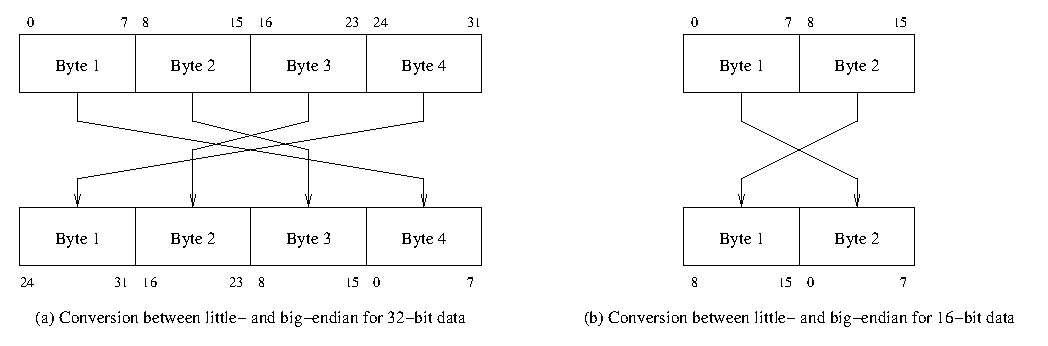
\includegraphics[scale=0.92]{byswpx}
  \end{center}
  \caption{Conversion between big- and little-endian
           \label{fig:cvt-big-ltl-end}}
\end{figure}
%-----------------------------------------------------------------------

It should be noted that the simple byte-swapping above does not work
properly for conversion of other multi-byte structures. For the
purposes of the STL, however, 16-bit structures is the most import
case. For several of the STL modules, the provided test files in
general need to be byte swapped in one or another computer
platform. The documentation and the ``manifesto'' accompaining each
software tool module describe which files, if any, should be
byte-swapped on certain platforms. As default, binary files organized
in 16-bit words are provided in big endian format in the STL
distribution.


%------------------------------------------------------------------------------
\section {Guidelines for software tool development} \hskip 1em \label{UGST-GLs}
%------------------------------------------------------------------------------

The software tools provided by the ITU-T User's Group on Software
Tools are to be used by laboratories with different computers and
A/D-D/A equipment. To make the software accessible to everybody, it
should be highly portable across operating systems and allow for easy
implementation in existing hardware environments.

To achieve this, some simple guidelines were followed in the
development of the tools. The following are the UGST guidelines used to
generate the official and beta releases of the ITU-T Software Tool Library.

\def\labelenumi{\roman{enumi}.}
\def\theenumi{\roman{enumi}}

\begin{enumerate}
\item All software should be written in ANSI C.

\item Features of the language whose representation may create
      side-effects should not be used (e.g. {\tt union}).

\item All variables must be declared and the types used in the
      declarations must be the least platform dependent. For example,
      the keyword {\tt int} must be avoided. Instead \short~ should be
      used for 16-bit integers and {\tt long} should be used for
      32-bit integers.

\item The software should not contain any input or output that may be
      system dependent (e.g. open, read and write file operations).
      Instead, data must be passed to the modules as parameters of
      function calls. This will allow each laboratory to integrate the
      modules with their own application software without changing the
      modules.  Interfaces to various file formats and user
      interaction can optionally be provided as example main
      programs\footnote{\SF Also called {\em ``demonstration
      programs''} in this manual.} that will not be a part of the
      library module and should contain the least possible amount of
      code.

\item Well defined digital signal formats should be used and
      documented for each module to allow the various modules to work
      together.

\item The interface to the file system should be made in a standard way,
      but only within the example programs.

\item The source code should be properly documented, with a standard
      header.

\item Modularity is encouraged in the software design. All modules
      are self-contained, i.e. global definitions should be avoided.

\item Each module should have an attached specification document
      explaining the function and use of the module, the level of
      detail depending on its complexity.

\item The software modules shall be distributed to interested
      laboratories for comments and testing before they are approved
      and included in the ITU-T Software Tools Library, to minimize
      the ocurrence of bugs and to assure conformance with related
      ITU-T Recommendations (when applicable). Two test procedures
      have been devised: compliance and portability.
\end{enumerate}
\def\labelenumi{\arabic{enumi}.}
\def\theenumi{\arabic{enumi}}

The {\em compliance procedure} (or compliance test) is to certify that
a given tool module fully complies with specifications, which should
be carried out by at least one organization other than the proponent
organization (or by a group of organizations, each one checking a
different subset of the specifications, such that all together cover
all the specifications). In order to minimize the probability of
systematic errors, these procedures should be defined by the verifying
organization(s) without input from the tool provider(s).

The {\em portability verification procedure} (or portability test) is
to certify that a given validated tool works on platforms other than
the one(s) where they were generated and validated.  In simple cases
these verification procedures could be just test vectors (e.g. speech
or noise files). It was also pointed out that problems may arise in
Unix platforms, due to the existence of several flavors of Unix
available today (this means that a verification procedure could be
valid in one Unix machine, but not in other).

Portability verification procedures should be provided by the
proponents and shall be run on at least two relevant operating systems
(DOS, UNIX). In the past, procedures for the VMS operating system used
to be required, however this operating system has become less
common. For DOS, the ``pure'' 16-bit mode has become less common, and
16-bit emulation window under a 32-bit version of MS Windows is now
prevalent. These facts affect the choice of compiler.

The following is a list of compilers used to test the portability of
tools in the STL, although not all tools were necessarily tested with
all compilers.

\begin{Descr}{25mm}
\item[\pbox{20mm}{\em HP/c89}] %\rulex{1mm}\\
        This is the {\tt c89} compiler that can be purchased from HP
        for use in HP-UX systems. For the STL, tests with this
        compiler were performed with HP-UX 9.05. \\

\item[\pbox{20mm}{\em HP/gcc}] %\rulex{1mm}\\
        This is the HP-UX port of the {\tt gcc} compiler. The specific
        version may differ from tool to tool. Versions used included
        gcc 2.7.2.2 for HP-UX 9.05 and gcc-2.95.2 for HP-UX 10.20. \\

\item[\pbox{20mm}{\em MSDOS/gcc}]
        This is the MSDOS-6.22 port of the {\tt gcc} compiler version
        2.6.3-DJGPP V1. This is a 32-bit compilation of the code,
        however using a 16-bit interface. Executables are not likely
        to run under Windows MS-DOS emulation window. Needs a run-time
        32-bit extender called {\tt go32.exe}. \\

\item[\pbox{20mm}{\em MSDOS/tcc}]
        This is the Borland Turbo C++ Version 1.00 {\tt tcc}
        compiler. \\

\item[\pbox{20mm}{\em MSDOS/bcc}]
        This is Borland C++ {\tt bcc} compiler. Versions used included
        3.0 and 4.5. \\

\item[\pbox{20mm}{\em Solaris/gcc}]
        This is the {\tt gcc} compiler version 2.95 running under
        Solaris 7, usually in a Sparc platform.\\

\item[\pbox{20mm}{\em SunOS/cc}]
        This is the basic {\tt cc} C compiler bundled in the SunOS
        distribution. For the STL, SunOS version 4.1.3 was used. \\

\item[\pbox{20mm}{\em SunOS/acc}]
        This is the licensed {\tt acc} C compiler sold by Sun
        Microsystems.  For the STL, SunOS version 4.1 was used. \\

\item[\pbox{20mm}{\em Win32/gcc}]
        This is the {\tt gcc} compiler version 2.95 running under
        Windows NT 4 SP 4 and with the CYGWIN Unix emulation
        interface. These executables need either the CYGWIN
        environment or the run-time library cygwin1.dll to run, and
        they are expected to work properly in a DOS emulation window
        under Windows 95/98 as well. This version will not run under
        native MS-DOS. \\

\item[\pbox{20mm}{\em Win32/cl}]
        This is the command-line {\tt cl} version 12.00.8168 C
        compiler of the MS Visual C V.6 SP3 running under the WinNT 4
        SP4 (the executables will also run in Windows
        95/\-98/\-SE/\-Me/\-2000). This version will not run under
        native MS-DOS. \\

\end{Descr}

%\newpage


\section {Software module I/O signal representation} \hskip 1em
%        =====================================================

The idea behind the choice of the convention in this section is that
all software modules within the ITU-T tool library should be
independent building blocks which can easily be combined by connecting
the output of one module to the input of the next module.  With this
characteristic, various systems may be very easily constructed. The
individual software modules must have well-defined interfaces to allow
such simple connections, especially at the I/O level. This convention
is based on the following:

\begin{enumerate}

\item All modules work `from RAM to RAM'. This means that the working
      modules are independent from physical I/O functions which are
      normally machine dependent.  This approach also allows easy
      cascading of modules within one `main' program.

\item All signals at the I/O interfaces of modules are represented in one
      of the following ways:

      \begin{enumerate}
        \item in single or double precision (32 or 64 bit) floating-point
              representation.  The normalized signal is used directly
              ({\em overload point = reference point = 1.0})

        \item in 32 bit 2's complement representation. The normalized signal
              must be multiplied by $\SF 2^{31}$ (i.e. the decimal
              point is just after the MSb, same as for 16 bit
              representation).  If less than 32 bits are required,
              then the signal is left adjusted within the 32 bit
              longword and the LSbs are optionally set to 0.

        \item in 16 bit 2's complement representation, as described in
              section \ref{ovl-point}.  If less than 16 bits are
              required, then the signal is left adjusted
              (left-justified) within the 16 bit words and the LSbs
              are optionally set to 0. If the host machine does not
              provide a format with 16 bit width, then the next
              longer wordlength should be used with the 16 bits right
              adjusted.
      \end{enumerate}

\item Data exchange with a module shall be done directly within the
      calling statement (not by global variables).

\item Data exchange with a module shall be done sample-by-sample
      (FIR-filtering, MNRU, etc.) or frame-by-frame (block oriented
      speech codec, etc.), whichever is more convenient. Larger
      blocks may be formed (e.g. 128 samples at a time) for better
      efficiency, however the block size should be rather small
      (less than 512). The block and its length shall be variables.

\item All modules shall be constructed in a way that infinitely long
      signals may be processed with a reasonable amount of internal storage.
      As an example, the `main' program could read a block of input
      data (e.g., next frame of time signal samples) from the disk,
      call a module or sequence of modules, write the output
      signal (e.g., next frame of coded parameters) back onto disk.
      This process is repeated for all the input data blocks of interest.

\item All modules shall have
      \begin{enumerate}
      \item an initialization part (if necessary) and
      \item a working part
      \end{enumerate}

      The initialization part may be necessary to reset internal
      state variables, define the mode of operation (e.g. MNRU-mode),
      and so on. It is called only once at the beginning or whenever
      a reset to an initial state is needed.

      \NOTE{140mm}{All state variables (if any) must
                be initialized at execution time, not at compile or
                load time.}

      The working part performs the processing itself. It leaves all
      state variables in a well-defined manner for the immediate use
      within the next call. One possible way to do this is to
      introduce a flag-variable within the call statement (e.g.,
      named `Initialize') which is set by the `main' program to '1'
      for initialization and is set to '0' during normal
      operation. In this way, only one function for one module is
      necessary.  Alternatively, a specialized initialization
      routine may be written, to be called before the main
      processing routine of the module. Only one of the approaches
      will be followed in the future. However, both are present in
      the current version of the STL.

\item The RAM allocation shall in principle be split into 'static' and
      'temporary' parts. `Static' means that the contents must be
      saved from call to call, preferrably by means of state variables
      rather than truly static variables\footnote{\SF As a rule, state
      variables should not be defined as truly static ones because
      this may cause side-effects.}. `Temporary' means that the
      contents are not saved between sucessive calls of the module.

\item All modules are separated in clearly and independently defined
      functions, but accompanied by an example `main' program which
      may also include file I/O.
\end{enumerate}


%------------------------------------------------------------------------------
\section {Tool specifications} \hskip 1em
%------------------------------------------------------------------------------

For each tool, there are `Requirements and Objectives' (\ROs)
associated. Each of the \ROs~ has both a general and a specific part.

The general part includes the following\footnote{\SF GL$x$~ refers to
the Guideline number $x$ in section~\ref{UGST-GLs}, e.g., GLiii is the
Guideline iii.}:

\begin{quote}
\begin{enumerate}
 \item Portability among platforms and Operating Systems (DOS, UNIX, and VMS):
        \begin{itemize}
         \item  compilation [GL-i];
         \item  usage of language features that may cause
                  side-effects [GL-ii];
         \item  usage of language  features  that may  be
                  ambiguous among platforms [GL-iii];
         \item  usage of system dependent calls (to access
                  resources such as files, etc.  within the
                  modules) [GL-iv];
        \end{itemize}

 \item Efficiency:
        \begin{itemize}
         \item  use of CPU (i.e., execution speed);
         \item  use of I/O (intensity of access to files, etc.);
         \item  use of memory (physical/virtual);
         \item  code's coverage (verbosity versus laconism);
        \end{itemize}

 \item Documentation:
        \begin{itemize}
         \item  Self-documentation (e.g., comments, variables and structure
                  resembling ITU-T Recommendations, etc.)[GL-vii];
         \item  Separate documentation (clarity, objectivity, etc.)[GL-ix];
        \end{itemize}

  \item Modularity [GL-viii]

  \item Fixed- versus floating-point implementations;
\end{enumerate}
\end{quote}


Following are descriptions of each of the General \ROs. Full
description of the \ROs~ can be found in \cite[Annex 4]{COM-XV-R-73-E}.

{\em General performance specification} refers to the
document that specifies the tool in question, e.g. an ITU-T
Recommendation or ANSI or ETSI standard.

{\em Portability} addresses several points related to the tool's
capacity of working on several platforms: {\em Compilation and
linkage} refers to the necessity of changes in the source code to make
a tool compile without any modification in a given environment.  It
was identified that the operating systems of most interest are DOS and
Unix (both BSD and System V). {\em Side-effectable features} are those
that, if used in a program, when changing one parameter, may cause
other(s) to be changed implicitly. {\em Ambiguous features} are those
that, due to the flexibility left in the C language specification, are
implemented in different ways for different platforms. For example,
{\tt int} in C is 32-bit wide in VAX-C and Unix workstations, but is
16-bit wide for most compilers available on MS-DOS
(Turbo-C/MS-C). {\em System-dependent calls} are calls that are
restricted to or are implementation of features of a particular
platform, to make better use of that particular computer architecture.

{\em Efficiency} is related to how the computer's resources
are used in terms of CPU, I/O and memory allocation, that may be a
burden and prevent the usage in some systems, either by lack of
resources or length of time needed for execution. Efficiency also
includes {\em code's coverage}, expressing how frequently code is
accessed.

{\em Documentation} refers to how to describe the tool. {\em
Self-documentation} is the documentation present in the program itself
to assure that the code clearly describes the algorithm
implemented, to provide compilation and linkage instructions, as well as
to report known bugs, etc. A {\em separate document} will
be mandatory when no written description of the algorithm is available,
or when the written documents that specify the tool are too general.

{\em Modularity degree} is the degree of isolation that a particular
tool has. From UGST Guidelines, all tools must be modular, i.e.,
self-contained blocks; nonetheless, tools may make use of system
resources other than memory and CPU.

{\em Arithmetic} is the number representation specification, either in
fixed (2's complement, 1's complement, etc.) or floating point. Here,
``fixed-point'' shall always be understood as 2's complement
representation, except where otherwise indicated.


%%=============================================================================
%\chapter{Tool x}
%%=============================================================================
%
%\section{Description}
%\section{Algorithm}
%\section{Implementation}
%\section{Examples}

%=============================================================================
% chapter G.711: The ITU-T 64 kbit/s log-PCM algorithm
%=============================================================================

%=============================================================================
% ...... THIS IS chapter{G.711: The ITU-T 64 kbit/s log-PCM algorithm } ......
% Revisions: 
% 04.Jan.1996 - Peter Kroon revision incorporated
% 22.Feb.2001 - Edits in example section
%
%=============================================================================
\chapter{G.711: The ITU-T 64 kbit/s log-PCM algorithm}
%=============================================================================

In the early 1960's an interest was expressed in encoding the analog signals
in telephone networks, mainly to reduce costs in switching and
multiplexing equipments and to allow the integration of communication
and computing, increasing the efficiency in operation and maintenance
\cite{Qual-meas-tel-sys}.

In 1972, the then CCITT published the Recommendation ITU-T G.711 that
constitutes the principal reference as far as transmission systems
are concerned \cite{G.711}. The basic principle of the algorithm is
to code speech using 8 bits per sample, the input voiceband signal
being sampled at 8 kHz, keeping the telephony bandwidth of
300--3400 Hz. With this combination, each voice channel requires
64 kbit/s.

\section{Description of the algorithm}

The idea behind the digitalization of the network involved a
compromise: use as far as possible the existing infrastructure; this imposes a
bandwidth limitation for the bit-streams of coded signals. A rate of 64
kbit/s was found to be reasonable.

If one thinks of using the most natural quantization scheme, one will
choose linear quantization. But one drawback of this approach is that
the signal-to-noise ratio (SNR) varies with the amplitude of the input
signals: the smaller the amplitude, the smaller the SNR. And, from the
quality point of view, if a signal has a wide variance, or a variance
that changes with time (as in the case of speech signals), the SNR
will also change, resulting in a wide-varying quality of the
system.

To avoid this problem, one can use logarithmic quantization, which
will result into a more uniform quantization noise. With this in
mind, several studies were carried out in late 1960's to choose a
good algorithm for this purpose. This led to the definition of two
transmission schemes, one using the $\mu$ law compression
characteristic: 
\[ 
   c(x) = x_{max} \frac{\ln(1 + \mu |x|/x_{max}) }{
                        \ln(1+\mu) } sgn(x) 
\] 
and the other using the A law compression characteristic: 
\[ 
   c(x) = \left \{ \begin{array}{ll}
          {\displaystyle A|x| \over \displaystyle 1 + \ln(A) } sgn(x), 
                &\mbox{for } 0 \leq \Frac{|x|}{x_{max}} \leq \Frac{1}{A}\\
          x_{max} {\displaystyle 1 + \ln(A|x|/x_{max}) \over 
                   \displaystyle 1 + \ln(A) } sgn(x),
                &\mbox{for \ruley{2em}} 
                   \Frac{1}{A} \leq \Frac{|x|}{x_{max}} \leq 1
          \end{array}
       \right .
\]

Both characteristics behave as linear for small amplitude signals
(being then equivalent to a linear quantization scheme), but are truly
logarithmic for large signals. In fact, for large signals the SNR is:
\[
    \mbox{\em SNR}_\mu = 6.02 B + 4.77 - 20 \log_{10} (\ln(1+\mu))
\]
and
\[
    \mbox{\em SNR}_A = 6.02 B + 4.77 - 20 \log_{10} (1 + \ln A)
\]
where $B$ is the number of bits used for quantization.

The ITU chose the values $A=87.56$ and $\mu=255$ for the G.711
standard, together with 8 bits per sample, what leads the latter two
equations to:
\[
    \mbox{\em SNR}_\mu = 6.02 B - 9.99 = 38.17 dB
\]
and
\[
    \mbox{\em SNR}_A = 6.02 B - 10.1 = 38.06 dB
\]

The G.711 standard does not specify the law as defined above, but
rather uses a good linear-piecewise approximation for 8 bit samples,
which has easier implementation (in hardware), as well as other
properties (see \cite[p.229]{Jayant-Noll}).

This approximation uses bit 1 for sign (1 for positive, 0 for
negative), bits 2--4 to indicate a segment, and bits 5--8 for
level\footnote{\SF Please note that the bit numbering in the G.711 is
the reversal of the commonly used in computer languages, G.711's bit 1
corresponding to common-sense's (most significant) bit 7, and G.711's
bit 8 to the normal least significant bit 0, respectively.}. Within
each segment, the quantization is linear (4 bits, or 16 levels), having
15 segments of distinct slopes for $\mu$ law, and 13 for A law.

The A law works with signals in the range from -4096 to 4096,
implying in a range of 13 bits. As for the $\mu$ law, the linear
signals are accepted in the range -8159 to 8159, which is represented
by 14 bits. Besides this, in the dynamic range sense, A and $\mu$ law
are equivalent to 12 and 13 bit linear quantization, respectively.

One detail for the A law is that the even bits are inverted. The reason
for this comes from problems observed (before the standardization of
the line code HDB3) in transmission systems when long sequences of
zeros happen, because small amplitudes, in A law, to be coded mostly
using `0' bits. With this bit-inversion, long sequences of bits `0'
becomes less probable, thus improving performance.

The conversion rule for A/$\mu$ law from/to linear is described in
terms of tables in G.711. A good reason for this is that there is no
closed form for the compression of linear samples (although it is
possible to find a closed formulae for the expansion algorithm). 
Hence, two implementations are possible: table look-up, and algorithmic.
For in-chip (LSI) implementations, the first one may be preferred,
because it is simpler to implement, at the cost of a wider chip area.
For other applications, such as using Digital Signal Processors (DSPs),
or software implementations, table look-up would occupy too much
memory, and the algorithmic solution would be preferred.

\section{Implementation}

This implementation of the G.711 can be found in the module {\tt
g711.c}, with prototypes in {\tt g711.h}.

For the reason explained before, an algorithmic approach to the G.711
was followed. For the compression routines, first the samples are
converted from two's complement to signed magnitude
notation\footnote{\SF Using the samples as two's complement in the
compression algorithm is a very common error whose effects are only
noticeable for small amplitude signals. Our approach agrees to the one
in G.726\cite{G.726}, block {\em compress}.}. So, a segment
classification is done, and then the linear quantization of a certain
number of bits of the input sample, that depends on the segment number
(e.g., for A law, segment 1 uses a factor of 2:1, 2 a 4:1, etc.) is
carried out. Finally, the sign of the sample is added. The expansion
routines are even simpler: find the sign, get the mantissa and the
exponent, and compute the linear sample.

One important point here is that, following UGST Guidelines, linear
input samples must be left-justified {\tt short}s. With this approach,
the knowledge of the 0 dB reference for the file is simplified, and the
need of having to apply different normalization factors to files if
they are to be coded by A or $\mu$ law is eliminated\footnote{\SF In
the case of stand-alone tools, this would mean that two copies of the
same file should be available!}. As an example, suppose that we want to
process a speech file $\cal X$ by the G.711 at an input level of -20
dBov for both A and $\mu$ law. Then, if the sample representation is
right-justified, and a factor $f$ brings a file's level to -20 dBov for
$\mu$ law, then for A law the factor will be $2.f$, due to the
difference in input signal's dynamic range of both laws (4096 and 8159,
respectively). On the other hand, if the samples are left-justified,
the factor is only one, and the routines will only look at the 13 or 14
most significant bits of the 16-bit word, for A and $\mu$ law,
respectively. In other words, the peak value for linear and A/$\mu$ law
is the same, therefore one factor is sufficient.

Compliance tests to this code have been done using a ramp file having
the full excursion of the dynamic range for each of the laws, and
examining the compressed and expanded samples against the values
expected in tables 1a, 1b, 2a, and 2b of Recommendation ITU-T G.711 (see
\cite{G.711}). Another test done exploits the synchronous property of
the G.711 scheme. Only samples from column 7 of G.711 tables 1 and 2
were used. These values are transparent to quantization. Hence, if
the coding was done properly, output samples should match exactly the
original ones.

The compression functions are {\tt alaw\_compress} and {\tt
ulaw\_compress}, and the expansion functions are {\tt alaw\_expand} and
{\tt ulaw\_expand}. In the next part you find a summary of calls to
these functions.

\subsection{{\tt alaw\_compress} and {\tt ulaw\_compress}}

{\bf Syntax: } 

{\tt
\#include "g711.h"\\
void alaw\_compress
         (\ttpbox{110mm}{
            long {\em smpno}, short {\em *lin\_buf}, short {\em *log\_buf})
         }\\
void ulaw\_compress
         (\ttpbox{110mm}{
            long {\em smpno}, short {\em *lin\_buf}, short {\em *log\_buf})
         }
}

{\bf Prototype: }       g711.h

{\bf Description: }

{\tt alaw\_compress} performs A law encoding rule according to
Recommendation ITU-T G.711, and {\tt ulaw\_compress} does the same for $\mu$
law. Note that input samples shall be left-justified, and that the
output samples are right-justified with 8 bits.

{\bf Variables: }
\begin{Descr}{\DescrLen}
\item[\pbox{20mm}{\em smpno}] %\rulex{1mm}\\
               Is the number of samples in lin\_buf.

\item[\pbox{20mm}{\em lin\_buf}] %\rulex{1mm}\\
               Is the input samples' buffer; each {\tt short} sample 
               shall contain linear PCM (2's complement, 16-bit wide) 
               samples, left-justified.

\item[\pbox{20mm}{\em log\_buf}] %\rulex{1mm}\\
               Is the output samples' buffer; each {\tt short} sample 
               will contain right-justified 8-bit wide valid A or $\mu$ 
               law samples. 
 
\end{Descr}
        
        {\bf Return value: }        None.


\subsection{{\tt alaw\_expand} and {\tt ulaw\_expand}}

{\bf Syntax: } 

{\tt
\#include "g711.h"\\
void alaw\_expand 
         (\ttpbox{110mm}{
            long {\em smpno}, short {\em *log\_buf}, short {\em *lin\_buf})
         }\\
void alaw\_expand 
         (\ttpbox{110mm}{
            long {\em smpno}, short {\em *log\_buf}, short {\em *lin\_buf})
         }
}

{\bf Prototype: }       g711.h

{\bf Description: }

{\tt alaw\_expand} performs A law decoding rule according to
Recommendation ITU-T G.711, and {\tt ulaw\_expand} does the same for $\mu$
law. Note that output samples will be left-justified, and that the
input samples shall be right-justified with 8 bits.

{\bf Variables: }
\begin{Descr}{\DescrLen}
\item[\pbox{20mm}{\em smpno}] %\rulex{1mm}\\
               Is the number of samples in log\_buf.

\item[\pbox{20mm}{\em log\_buf}] %\rulex{1mm}\\
               Is the input samples' buffer; each {\tt short} sample 
               shall contain right-justified 8-bit wide valid A or $\mu$ 
               law samples.

\item[\pbox{20mm}{\em lin\_buf}] %\rulex{1mm}\\
               Is the output samples' buffer; each {\tt short} sample 
               will contain linear PCM (2's complement, 16-bit wide) 
               samples, left-justified.

\end{Descr}
        
        
        {\bf Return value: }        None.


\section{Tests and portability}  

Portability may be checked by running the same speech file in a
proven platform and in a test platform. Files processed this way
should match exactly. Source and processed reference files for
portability tests are provided in the STL distribution.

These routines had portability tested for VAX/VMS with VAX-C and gcc, 
MS-DOS with Turbo C v2.0, HPUX with gcc, and Sun-OS with Sun-C.


%-----------------------------------------------------------------
\section{Example code}

%.................................................................
\subsection {Description of the demonstration program}

One program is provided as demonstration program for the G.711 module,
g711demo.c.

Program {\tt g711demo.c} accepts input files in 16-bit linear PCM
format for compression operation and produces files in the same format
after the expansion operation. The compressed signal will be in
16-bit, right adjusted format, according to the logarithmic law
specified by the user. Three operations are possible: linear in,
linear out ({\em lili}) linear in, logarithmic out ({\em lilo}), or
logarithmic in, linear out ({\em loli}).

%.................................................................
\subsection {Simple example}

The following C code gives an example of companding using either the
A- or $\mu$-law functions available in the STL. 

{\tt\small 
\begin{verbatim}
#include <stdio.h> 
#include "ugstdemo.h" 
#include "g711.h"

#define BLK_LEN 256
#define QUIT(m,code) {fprintf(stderr,m); exit((int)code);}

main(argc, argv)
  int             argc;
  char           *argv[];
{
  char            law[4];

  char            FileIn[180], FileOut[180];
  short           tmp_buf[BLK_LEN], inp_buf[BLK_LEN], out_buf[BLK_LEN];
  FILE           *Fi, *Fo;
  void          (*compress)(), (*expand)(); /* pointer to a function */

  /* Get parameters for processing */
  GET_PAR_S(1, "_Law (A,u): ................... ", law);
  GET_PAR_S(2, "_Input File: .................. ", FileIn);
  GET_PAR_S(3, "_Output File: ................. ", FileOut);

  /* Opening input and output LOG-PCM files */
  Fi = fopen(FileIn, RB);
  Fo = fopen(FileOut, WB);

  /* Choose compression/expansion routinies according to the law */
  if (toupper(law[0])=='A')
  {
     compress = alaw_compress;
     expand = alaw_expand;
  }
  else if (tolower(law[0])=='u')
  {
     compress = ulaw_compress;
     expand = ulaw_expand;
  }
  else 
    QUIT("Bad law chosen!\n",1);

 /* File processing */
  while (fread(inp_buf, BLK_LEN, sizeof(short), Fi) == BLK_LEN)
  {
    /* Process input linear PCM samples in blocks of length BLK_LEN */
    compress(BLK_LEN, inp_buf, tmp_buf);

    /* Process log-PCM samples in blocks of length BLK_LEN */
    expand(BLK_LEN, tmp_buf, out_buf);

    /* Write PCM output word */
    fwrite(out_buf, BLK_LEN, BLK_LEN, sizeof(short), Fo);
  }

  /* Close input and output files */
  fclose(Fi);
  fclose(Fo);
  return 0;
}
\end{verbatim}
}


%=============================================================================
% chapter G.711: G.711 Appendix I: A high quality low-complexity algorithm
% for packet loss concealment with G.711.
%=============================================================================
%=============================================================================
% ..... THIS IS chapter{TRUNCATE: ITU-T bitstream truncation tool } .....
%     Apr.2005
% ... Authors :
%        Cyril Guillaum� & St�phane Ragot - stephane.ragot@francetelecom.com
% Apr.2005 - Created
% Oct.2005 - Editorial changes (Simao Campos)
%=============================================================================
\chapter{G.711 Appendix I: A high quality low-complexity 
algorithm for packet loss concealment with G.711.}
%=============================================================================

%----------------------------------------------------------------------
\section{Introduction}
%----------------------------------------------------------------------

Packet Loss Concealment (PLC) algorithms hide transmission losses in
audio systems where the input signal is encoded and packetized at a
transmitter, sent over a network, and received at a receiver that
decodes the packet and plays out the output. G.711 Appendix I
\cite{G711-appendix-I}, approved by ITU-T in September 1999, describes
a high quality, low complexity PLC algorithm designed for use with
G.711.

%----------------------------------------------------------------------
\section{Description of the algorithm}
%----------------------------------------------------------------------

A brief description of the PLC algorithm is given. A more extensive
presentation can be found in Section I.2, ``Algorithm description'',
of G.711 Appendix I \cite{G711-appendix-I}.

The PLC algorithm is inserted after the G.711 decoder at the
receiver. The algorithm is designed to work with 10 ms frames, or 80
samples per frame at 8 KHz sampling. An external mechanism is needed
to signal when packets are lost. Since speech signals are often
locally stationary, the signals recent history is used to generate a
reasonable approximation to lost frames. If the losses are not too
long, and do not land in a region where the signal is rapidly
changing, the losses may be inaudible after concealment.

When a frame is received the decoded speech is given to the PLC
algorithm. Received frames are saved in a 48.75 ms circular history
buffer, and the output is delayed by 3.75 ms (30 samples).

When a packet is lost the concealment algorithm starts synthetic
signal generation. First the pitch is estimated by finding the peak
of the normalized autocorrelation of the most recent 20 ms of speech
in the history buffer with the previous speech at taps from 5 to 15
ms. Using the pitch estimate, the most recent pitch period from the
history buffer is repeated for the duration of the first lost frame
(10 ms). If the pitch estimate is longer than 10 ms, only a portion
of the most recent pitch period will be used in the first lost
frame. A 1/4 pitch period overlap add (OLA) with a triangular window
is performed at all repetition boundaries, including the transition
between the last received frame and the start of the synthetic
signal.

If consecutive frames are lost, the number of pitch periods used to
generate the synthetic signal is increased by one pitch period at
the start of the 2nd and 3rd lost frames. When the number of pitch
periods is increased, the output is smoothly transitioned to the
oldest used pitch period of the history signal with an additional
1/4 pitch period OLA. Increasing the number of pitch periods reduces
the number of unnatural harmonic artifacts in the concealed speech
for long losses. The algorithm does not distinguish between voiced
and un-voiced speech and uses the same procedure for both types of
speech.

At the start of the first received frame after a loss, the synthetic
signal generation is continued and OLAed with the received speech.
This OLA window length increases with the length of the loss. For
single frame losses it is 1/4 of the estimated pitch period. 4 ms
are added for each additional consecutive lost frame, up to a
maximum of 10 ms.

If the loss exceeds 10 ms the synthetic signal is also linearly
attenuated at the rate of 20\% per frame. If the loss exceeds 60 ms
the synthesized signal is set to silence.


%----------------------------------------------------------------------
\section{Implementation}
%----------------------------------------------------------------------

%-.-.-.-.-.-.-.-.-.-.-.-.-.-.-.-.-.-.-.-.-.-.-.-.-.-.-.-.-.-.-.-.-.-.-.
\subsection{Introduction}

The g711iplc directory contains an ANSI C implementation of the
G.711 Appendix I PLC algorithm. The C++ version of this algorithm is
in the g711iplc$\setminus$cpp\_cod directory. Sample test programs
read lost frame patterns in G.192 file format and apply the PLC
algorithm to audio files. The software in the g711iplc directory is
covered by a more restrictive copyright than the STL. See the
copyrght.txt file for details.

%Here is a summary of the files in the g77iplc directory:
%\begin{Descr}{70mm}
%    \item[\pbox{40mm}{lowcfe.h, lowcfe.c}] ANSI C implementation of the PLC algorithm
%    \item[\pbox{40mm}{g711iplc.c}] ANSI C test program for PLC algorithm
%    \item[\pbox{40mm}{plcferio.h, plcferio.c}] Routines for reading G.192 format pattern files
%    \item[\pbox{40mm}{error.h, error.c}] Error handling routine
%    \item[\pbox{40mm}{makefile.cl}]     Makefile file for Visual C++ on Windows
%    \item[\pbox{40mm}{copyrght.txt}] The software (c) Copyright
%\end{Descr}

%-.-.-.-.-.-.-.-.-.-.-.-.-.-.-.-.-.-.-.-.-.-.-.-.-.-.-.-.-.-.-.-.-.-.-.
\subsection{PLC Algorithm Implementation}

A detailed line by line description of the C++ code can be found in
section I.3 ``Algorithm description with annotated C++ code'' of G.711
Appendix I \cite{G711-appendix-I} and will not be repeated here. The
public interface functions that are called by applications are
covered. The C++ version is in the g711iplc$\setminus$cpp\_code
directory (files lowcfe.h and lowcfe.cc). The ANSI C version,
contained in the files lowcfe.h and lowcfe.c, is a translation of
the C++ code to C. The interface functions are the same for both
versions, with the exception that the C versions of the routines
take an extra argument for the data structure that is implicitly
passed to C++ member functions in the class instance data. As for
other STL modules, only the ANSI C version is compiled during
STL2005 building.

%\enlargethispage*{20mm}

%-.-.-.-.-.-.-.-.-.-.-.-.-.-.-.-.-.-.-.-.-.-.-.-.-.-.-.-.-.-.-.-.-.-.-.
\mysubsubsection{Constructor}

{\bf C++ syntax: }

{\tt \#include "lowcfe.h" \\
LowcFE  {\em{lc}}; // No argument constructor}

{\bf C syntax: }

{\tt \#include "lowcfe\_c.h" \\
g711plc\_construct({\em{LowcFE\_c*}}); /* explicit constructor call */}

{\bf Description: }

Before the PLC algorithm can be called the data structure containing
the algorithm's internal storage, such as the history buffer and
buffer pointers, must be initialized.

%-.-.-.-.-.-.-.-.-.-.-.-.-.-.-.-.-.-.-.-.-.-.-.-.-.-.-.-.-.-.-.-.-.-.-.
\mysubsubsection{Received Frames}

{\bf C++ syntax: }

{\tt void LowcFE::addtohistory(short {\em{*s}}); /* add a frame to
the history buffer */}

{\bf C syntax: }

{\tt void g711plc\_addtohistory({\em{LowcFE\_c*}}, short
{\em{*s}});}

{\bf Description: }

Frames of speech received from the transmitter are given to the PLC
algorithm with {\tt addtohistory} function. The argument {\em{s}}
points to a short array of length FRAMESZ (80 samples, or 10 ms)
that is used as both an input and output. Before the call is made
{\em{s}} is filled with the decoded G.711 data received from the
transmitter. On return, it contains the data that is output to the
listener. Addtohistory performs several operations. It stores the
input speech into the history buffer for use in generating the
synthetic signal if a loss occurs. If this is the first received
frame after a loss, an OLA is performed with the synthetic signal to
insure a smooth transition between the signals. In addition, it
delays the output so an OLA can be performed at the start of a loss.

%-.-.-.-.-.-.-.-.-.-.-.-.-.-.-.-.-.-.-.-.-.-.-.-.-.-.-.-.-.-.-.-.-.-.-.
\mysubsubsection{Lost Frames}

{\bf C++ syntax: }

{\tt void LowcFE::dofe(short {\em{*s)}};    /* synthesize speech
during loss */}

{\bf C syntax: }

{\tt void g711plc\_dofe({\em{LowcFE\_c*}}, short {\em{*s}});}

{\bf Description: }

If a frame is lost, the dofe routine is called. As with {\tt
addtohistory}, {\em{s}} is a pointer to short array of FRAMESZ
samples. With dofe, {\em{s}} is only an output. The PLC algorithm
fills {\em{s}} with the synthetic signal that conceals the missing
frame.

%-.-.-.-.-.-.-.-.-.-.-.-.-.-.-.-.-.-.-.-.-.-.-.-.-.-.-.-.-.-.-.-.-.-.-.
\mysubsubsection{Support Functions}

{\tt error}

{\bf Syntax: }

{\tt \#include "error.h" \\
void error\ttpbox{130mm}{(char {\em{*s}}, ...);}}

{\bf Description: }

Error handles fatal errors in the programs. The pattern string,
{\em{s}}, and optional following arguments should be in the format
of arguments accepted by the C library printf function. Error prints
its argument message on stderr and then exits the program. The error
function never returns.

{\tt readplcmask\_open}

{\bf Syntax: }

{\tt \#include "plcferio.h"\\
 void readplcmask\_open\ttpbox{130mm}{(readplcmask {\em{*r}},
char {\em{*fname}});}}

{\bf Description: }

The {\tt readplcmask\_open} function opens a G.192 format file
containing a packet loss pattern. {\em{fname}} is the file path. If
successfully opened, {\em{r}} contains the state information needed
for reading the patterns. {\tt readplcmask\_open} internally calls
the STL eid module to determine the type of the G.192 file and
select an appropriate reading function. If the open fails or an
unknown pattern is detected in the file, function {\tt error} is
called and {\tt readplcmask\_open} will not return.

{\tt readplcmask\_erased}

{\bf Syntax: }

{\tt \#include "plcferio.h"\\
int readplcmask\_erased\ttpbox{130mm}{(readplcmask {\em{*r}});}}

{\bf Description: }

{\tt readplcmask\_erased} reads the next value from the opened G.192
format pattern file. It returns 1 if the frame is lost and should be
concealed and 0 if the frame is ok. If the end of the G.192 file is
reached, the routine seeks back to the beginning of the file and the
pattern sequence is repeated. If an illegal value is found in the
G.192 file, the error function is called.

{\tt readplcmask\_close}

{\bf Syntax: }

{\tt \#include "plcferio.h"\\
void readplcmask\_close\ttpbox{130mm}{(readplcmask {\em{*r}})}}

{\bf Description: }

{\tt readplcmask\_close} is used to close a G.192 file that was
opened with {\tt readplcmask\_open}.

%-.-.-.-.-.-.-.-.-.-.-.-.-.-.-.-.-.-.-.-.-.-.-.-.-.-.-.-.-.-.-.-.-.-.-.
\subsection{Test Program}
%-...-...-...-...-...-...
\mysubsubsection{Test Program Usage}

The PLC algorithm is tested using g711iplc.c. The PLC test programs
take 3 file arguments:

\rulex{1cm}  {\tt g711iplc mask.g192 input.raw output.raw}

The {\tt mask.g192} file contains the lost frame pattern and should
be in the G.192 format as specified in the software tools library.
The g192, byte, and compact representations are supported. The G.192
file should contain only the frame headers words (G192\_SYNC or
G192\_FER, see softbit.h), and not the data words.

A frame corresponds to 10 ms, or 80 samples. If the lost frame
pattern file is shorter than the number of frames in the {\tt
input.raw} file, the program will roll-over back to the start of the
pattern file.  For example if the {\tt mask.g192} file contains the
binary data:
{\tt\small
\begin{verbatim}
    0x6B21 0x6B21 0x6B21 0x6B21 0x6B21,
    0x6B21 0x6B21 0x6B21 0x6B21 0x6B20
\end{verbatim}}
a 10\% uniform loss pattern will be applied to the whole file.
Erasures will occur at 90-100 ms, 190-200 ms, 290-300 ms ... in the
file.

While the algorithm is designed for packets containing 10ms of
speech, it can be applied to packetizations containing speech chunks
that are integer multiples of 10ms. For example, for a 10\% uniform
loss pattern with 20ms packetization one could use:

{\tt\small
\begin{verbatim}
    0x6B21 0x6B21 0x6B21 0x6B21 0x6B21,
    0x6B21 0x6B21 0x6B21 0x6B21 0x6B21,
    0x6B21 0x6B21 0x6B21 0x6B21 0x6B21,
    0x6B21 0x6B21 0x6B21 0x6B20 0x6B20
\end{verbatim}}
to cause erasures at 180-200ms, 380-400ms, 580-600ms, etc.

The input audio file, {\tt input.raw}, should contain header-less
16-bit binary data, sampled at 8 KHz, in the native byte order for
the machine running the test programs (big-endian on SPARC or MIPS,
little-endian on Intel). The test programs do not contain the G.711
encoder or decoder. If you have a G.711 bit-stream, it must be
decoded before the {\tt g711iplc} program is run.

The output audio file, {\tt output.raw}, also contains header-less
16-bit binary data. The PLC algorithm delays the output by 3.75 ms.
The test programs compensate for this delay by not outputting the
first 3.75 ms of the first packet. This way the input and output
files will be time aligned if they are overlaid in an audio waveform
editor. In addition, after the last full packet is input to the PLC
algorithm, an extra zero filled frame is input, and the first 3.75
ms of the corresponding output frame is sent to the output file. The
length of the output file will always be a multiple of the 10ms
frame size. If the input file length is not an integral number of
frames the last partial input frame will be discarded.

The test programs can also simulate a silence insertion algorithm
instead of the PLC algorithm with the {\tt -nolplc} option:

\rulex{1cm}  {\tt g711iplc -noplc mask.g192 input.raw output.raw}

Instead of calling the concealment algorithm the lost frames are
simply zero filled. This is helpful if you want to use a wave editor
to view the location of the missing frames.

Use the {\tt -stats} option to print out the number and percentage
of frames concealed in the processed file.

%-.-.-.-.-.-.-.-.-.-.-.-.-.-.-.-.-.-.-.-.-.-.-.-.-.-.-.-.-.-.-.-.-.-.-.
\mysubsubsection{Test Program Implementation}

A simplified version of the C++ test program is shown next. This
program does not support any options, such as -noplc, or compensate
for the algorithm delay, but demonstrates how the components work
together.

\newpage
{\tt\small
\begin{verbatim}
#include <stdlib.h>
#include <stdio.h>
#include <string.h>
#include "error.h"
#include "plcferio.h"
#include "lowcfe.h"

int main(int argc, char *argv[]) {
    FILE        *fi;        /* input file */
    FILE        *fo;        /* output file */
    LowcFE      fesim;      /* PLC simulation class */
    readplcmask mask;       /* error pattern file reader */
    short       s[FRAMESZ]; /* i/o buffer */

    argc--; argv++;
    if (argc != 3)
        error("Usage: g711iplc plcpattern speechin speechout");
    readplcmask_open(&mask, argv[0]);
    if ((fi = fopen(argv[1], "rb")) == NULL)
        error("Can't open input file: %s", argv[1]);
    if ((fo = fopen(argv[2], "wb")) == NULL)
        error("Can't open output file: %s", argv[2]);
    while (fread(s, sizeof(short), FRAMESZ, fi) == FRAMESZ) {
        if (readplcmask_erased(&mask))
            fesim.dofe(s);      /* lost frame */
        else
            fesim.addtohistory(s);  /* received frame */
        fwrite(s, sizeof(short), FRAMESZ, fo);
    }
    fclose(fo);
    fclose(fi);
    readplcmask_close(&mask);
    return 0;
}
\end{verbatim}
}

%-.-.-.-.-.-.-.-.-.-.-.-.-.-.-.-.-.-.-.-.-.-.-.-.-.-.-.-.-.-.-.-.-.-.-.
\subsection{Loss Pattern Conversion Utility}

The PLC directory includes a tool, {\tt asc2g192}, for converting
ASCII loss pattern files containing sequences of 0s and 1s into
G.192 format pattern files. In ASCII loss pattern files, a ``1''
represents a lost frame and a ``0'' represents a received frame. For
example, to create a 10\% uniform loss pattern with each loss being
10ms, use a text editor to create a text file called {\tt fe10.txt}:
{\tt\small
\begin{verbatim}
  0000000001
\end{verbatim}}
Then, convert it to the G.192 format for use by the g711iplc program
with the following command:
{\tt\small
\begin{verbatim}
  asc2g192 fe10.txt fe10.g192
\end{verbatim}}
Similarly, to create a 10\% uniform loss pattern with each loss
being 20ms (2 frames for each loss), create the text file {\tt
fe10\_2.txt} :
{\tt\small
\begin{verbatim}
  00000000000000000011
\end{verbatim}}
Then convert it to the G.192 format with:
{\tt\small
\begin{verbatim}
  asc2g192 fe10\_2.txt fe10\_2.g192
\end{verbatim}}
The {\tt asc2g192} conversion program ignores new lines and carriage
returns in the input file so the patterns can span multiple lines.


%=============================================================================
% chapter G.726: The ITU-T ADPCM algorithm
%=============================================================================
%=============================================================================
% ..... THIS IS chapter{G.726: The ITU-T ADPCM algorithm } .....
% ... Revision:
% Ago.1992 - M.Sheriff suggestions
% Ago.1992 - Some stilish changes
% Sep.1992 - M.Sheriff further suggestions
% Jan.1995 - Some changes in the call for the routines
% Oct.1995 - Replaced some references to G.721 to G.726
% Jan.1996 - Peter Kroon revision incorporated
% Feb.2000 - Convergence towards STL2000
% Feb.2001 - Edits in example section
%=============================================================================
\chapter{G.726: The ITU-T ADPCM algorithm at 40, 32, 24, and 16 kbit/s}
%=============================================================================

In 1982, a group was established by the then CCITT Study Group XVIII
to study the standardization of a speech coding technique that could
reduce the 64 kbit/s rate used in digital links, as per
Recommendation ITU-T G.711 (see related Chapter), by half while
maintaining the same voice quality.

After considering contributions received from several organizations, there was
a general feeling that the ADPCM {\em (Adaptive Differential Pulse Code
Modulation)} technique could provide a good quality coder. This process
of finalizing an algorithm took 18 months of development and objective
and subjective testings, to culminate in an ITU Recommendation,
published in October, 1984, and available in the Red Book series as
Recommendation ITU-T G.721.

Meanwhile, problems were found with the G.721 algorithm of 1984
regarding voice-band data signals modulated using the Frequency Shift
Keying (FSK) technique, and changes had to be done to the algorithm.
These changes were approved in 1986 and published in the next series of
Recommendations of the CCITT, the Blue Book series, superseeding the
Red Book version of the G.721. This is why a note in the Blue Book
G.721 warns the user that the bit stream of coded speech from this
version is incompatible with the old one. Also in that Study Period
(1985-1988), a need for other rates was identified, and a new
Recommendation, ITU-T G.723, was approved to extend the bitrate to 24 and 40
kbit/s.

In the Study Period of 1989--1992, these two Recommendations have been
joined into a single one, keeping full compatibility with the former
ones, and adding a lower rate of 16 kbit/s. This new Recommendation was
named ITU-T G.726, and the former ITU-T G.721 and G.723 have been replaced.

The current version of the STL includes a G.726 implementation. In the
section to follow, the operation of the G.726 algorithm is described
only for the 32 kbit/s bit rate. A complete description of the G.726
algorithm can be found in \cite{G.726}. Other analyses of the
algorithm, besides some based on the Red Book version, can be found in
several studies \cite{ADPCM-theor,ADPCM-over,ADPCM-Tech-Report}.

Despite the change in numbering, the ITU-T ADPCM algorithm for speech
coding at 32 kbit/s, the term ``G.721 algorithm'' has been retained
for simplicity of the text, although a more formal reference
should be {\em ``G.726 at 32 kbit/s''}.

\section{Description of the 32 kbit/s ADPCM}

The basic idea behind the G.721 coder is to code into 4-bit samples the
input speech-band signals, sampled at 8 kHz and represented by the
8-bit of G.711 A or $\mu$ law samples. The decoder just implements the
reverse procedure.

The ADPCM algorithm of the G.721 exploits the predictability of the
speech signals. Therefore, an adaptive predictor is used to compute the
difference signal $d(k)$ (based on the expanded input log-pcm sample
$s(k)$), which is then quantized by an adaptive quantizer using 4 bits.
These bits are sent to the decoder and then fed into an inverse
quantizer. The difference signal is used to calculate the reconstructed
signal, $s_r(k)$, which is compressed (A- or $\mu$-law) and output from
the decoder ($s_d(k)$).

From this description, one could ask the following:

\rulex{5mm}\begin{minipage}{140mm}
 $\bullet$ If only the quantized signal is transmitted, how can the
        decoder reconstruct  \rulex{2.5ex} the signal?

 $\bullet$ How can one assure estability of the predictor?

 $\bullet$ Will this bitrate reduction degrade the voice quality?
\end{minipage}

These and others have already been considered in the design of the
G.721, and many blocks of the algorithm are made to assure a good
behaviour. For example, one possibility in this backward approach for
adaptation is to have encoder and decoder starting from the same point,
which is accomplished by reseting key variables to a known state
(useful for implementation verification). Leak factors have been
introduced to ensure that the algorithm will always converge,
independently of the initial state. To avoid instabilities, some
parameters had their range limited. To provide some insight in the
building blocks of the G.721 algorithm, a short description of each of
them is given \cite{G.726,ADPCM-over}.


\subsection{PCM format conversion}

The input signal $s(k)$, in either A- or $\mu$-law format, must be
converted into linear samples. This expansion is accomplished using the
same algorithm in G.711 \cite{G.711}, but converting from signed
magnitude to 14-bit two's complement samples.


\subsection{Difference Signal Computation}

This block simply calculates the difference between the (expanded) input signal and the estimated signal:
\[
      d(k) = s_l(k) - s_e(k)
\]


\subsection{Adaptive Quantizer}

A 15-level, non-uniform adaptive quantizer is used to quantize the
difference signal. Before the quantization, this signal is converted to
a logarithmic representation\footnote{\SF Remember that to multiply
samples in the linear domain one may add in the logarithmic one. Using
efficient log and exponentiation algorithms (as done here), this turns
out to be very advantageous.} and scaled by a factor ($y(k)$), that is
computed in the scale factor adaptation block (see below).

The output of this block is $I(k)$, and it is used twice; first, is
the ADPCM coded ({\em quantized}) sample; second, is the input to the
backward part of the G.721 algorithm, to provide information for
quantization of the next samples. One relevant point to notice here
is that the backward adaptation is done using the quantized sample.
If one starts the decoder from this very point, one will find
identical behaviour. That is why only the  quantized samples are
needed in the decoder (i.e., no side information).


\subsection{Inverse Adaptive Quantizer}

The inverse adaptive quantizer takes the signal $I(k)$ and converts it
back to the linear domain, generating a quantized version of the
difference signal, $d_q(k)$. This is the input to the adaptive
predictor, such that the estimated signal is based on a quantized
version of the difference signal, instead of on the unquantized
(original) one.


\subsection{Quantizer Scale Factor Adaptation}

This block computes $y(k)$, the factor used in the adaptive quantizer
and inverse quantizer for domain conversion. As input, this block
needs $I(k)$, but also $a_l(k)$, the adaptation speed control
parameter. The reason for the latter is that the scaling algorithm
has two modes ({\em bimodal adaptation}), one fast, another slow.
This has been done to accomodate signals that in nature produce
difference signals with large fluctuations (e.g. speech) and small
fluctuations (e.g. tones and voice-band data), respectively.

This block computes two scale factor (fast, $y_u(k)$, and slow,
$y_l(k)$) based on $I(k)$, which combined using $a_l(k)$ produce
$y(k)$.


\subsection{Adaptation Speed Control}

This block evaluates the parameter $a_l(k)$, which can be seen as a
{\em proportion} of the speed (fast or slow) of the input signal, and
is in the range $[0,1]$. If 0, the data are considered to be {\em
slowly} varying; if 1, they are considered to be {\em fast}
varying.

To accomplish this, two measures of the average magnitude of $I(k)$ are
computed ($d_{ms}(k)$ and $d_{ml}(k)$). These, in conjunction with
delayed tone detect and transition detect flags ($t_d(k)$ and $t_r(k)$,
calculated in the Tone Transition and Detector block), are used to
evaluate $a_p(k)$, whose delayed version ($a_p(k-1)$) is used in the
definition of $a_l(k)$, limiting the range to $[0,1]$\footnote{\SF This
limitation delays the start of a fast to slow transition until the
average magnitude of $I(k)$ remains constant for some time; acting so,
premature transitions for pulsed input signals, such as switched
carrier voiceband data, are avoided.}.

An analysis of $a_p(k)$ gives insight on the nature of the signal: if
around the value of 2, this means that the average magnitude of $I(k)$
is changing, or that a tone has been detected, or that it is idle
channel noise; on the other side, if near 0, the average magnitude of
$I(k)$ remains relatively constant.


\subsection{Adaptive Predictor and Reconstructed Signal Calculator}

The adaptive predictor has as its main function to compute the signal
estimate based on the quantized difference signal, $d_q(k)$. It has 6
zeroes and 2 poles, structure that covers well the kind of input
signals expected for the algorithm. With these coefficients, and past
values of $d_q(k)$ and $s_e(k)$, the updated value for the signal
estimate $s_e(k)$ is computed.

The two sets of coefficients (one for the pole section, $a_i(k),
i=1..2$, other for the zero section, $b_i(k), i=1..6$) are updated
using a simplified gradient algorithm. At this point, since a situation
in which the poles cause instability may arise, the two pole
coefficients $a_i$ have their ranges limited. In addition, if a
transition from partial band signal is detected (signaled by $t_r(k)$),
the predictor is reset (all coefficients are set to 0), remaining
disabled until $t_r$ comes back to zero\footnote{\SF Note that when
this happens, the quantizer is forced into the fast mode of
adaptation.}.

The reconstructed signal $s_r(k)$ is calculated using the signal
estimate $s_e(k)$ and the quantized difference signal $d_q(k)$.


\subsection{Tone Transition and Detector}

This block is one of the changes from the Red Book version. It was
added to improve algorithm performance for signals originating from
FSK modems operating in the character mode.  First, it checks if the
signal has partial band (e.g., a tone) by looking at the predictor
coefficient $a_2(k)$, that defines the signal $t_d(k)$.  Second, a
transition from partial band signal indicator $t_r(k)$ is set, such
that predictor coefficients can be set to 0 and the quantizer can be
forced into the fast mode of operation.

\subsection{Output PCM Format Conversion}

This block is unique to the decoder. Its sole function is to compress
the reconstructed signal $s_r(k)$, which is in linear PCM format, using
A or $\mu$ law, and is a complement of the PCM format conversion
block.


\subsection{Synchronous Coding Adjustment}

This block is also unique to the decoder. It has been devised in order
to prevent cumulative distortions occuring on synchronous tandem
codings (ADPCM--\-PCM--\-ADPCM, etc., in purely digital connections, i.e.,
with no intermediate analog conversions), provided that:

\rulex{5mm} $\bullet$ \parbox[t]{140mm}{
               the transmission of the ADPCM and the intermediate PCM are
               error-free, and }

\rulex{5mm} $\bullet$ \parbox[t]{140mm}{
               the ADPCM and the intermediate PCM are not disturbed by digital
               signal processing devices.}

\subsection{Extension for linear input and output signals}

An extension of the G.726 algorithm was carried out in 1994 to include, as
an option, linear input and output signals. The specification for such linear
interface is given in its Annex A \cite{G.726:LinearIO}.

This extension bypasses the PCM format conversion block for linear input
signals, and both the Output PCM Format Conversion and the Synchronous
Coding Adjustment blocks, for linear output signals. These linear versions
of the input and output signals are 14-bit, 2's complement samples.

The effect of removing the PCM encoding and decoding is to decrease the
coding degradation by 0.6 to 1 qdu, depending on the network configuration
considered (presence or absence of a G.712 filtering).

Currently, this extension has not been incorporated in the STL.


\section{ITU-T STL G.726 Implementation}

The STL implementation of the G.726 algorithm can be found
in module {\tt g726.c}, with prototypes in {\tt g726.h}.

Originally in Fortran (VAX Fortran-77), the source was translated by means
of the public-domain code converter {\em f2c} \cite{f2c}. This explain why
the code makes extensive use of passage of parameters by reference, rather
than by value, and why many functions, that could be implemented as macros
(using the C pre-processor directive {\tt \#define}), are routines, and as
well as all routines return {\tt void}.

The problem of storing the state variables was solved by defining a
structure containing all the necessary variables, defining a new type
called {\tt G726\_state}. By means of this approach, several streams
may be processed in parallel, provided that one structure is assigned
(and that one call to the encoding/decoding routines is done) for
each data stream (this can be advantageous for machines with support
for parallel processing). The G726 state variable  structure has the
following fields (all are {\tt short}, except {\em ylp},  which is
{\tt long}):

\begin{quote} \normalsize
 {\em sr0} \hfill \pbox{120mm}{ Reconstructed signal with delay 0}\\
 {\em sr1} \hfill \pbox{120mm}{ Reconstructed signal with delay 1}\\
 {\em a1r} \hfill \pbox{120mm}{ Delayed 2nd-order predictor coefficient 1}\\
 {\em a2r} \hfill \pbox{120mm}{ Delayed 2nd-order predictor coefficient 2}\\
 {\em b1r} \hfill \pbox{120mm}{ Delayed 6th-order predictor coefficient 1}\\
 {\em b2r} \hfill \pbox{120mm}{ Delayed 6th-order predictor coefficient 2}\\
 {\em b3r} \hfill \pbox{120mm}{ Delayed 6th-order predictor coefficient 3}\\
 {\em b4r} \hfill \pbox{120mm}{ Delayed 6th-order predictor coefficient 4}\\
 {\em b5r} \hfill \pbox{120mm}{ Delayed 6th-order predictor coefficient 5}\\
 {\em b6r} \hfill \pbox{120mm}{ Delayed 6th-order predictor coefficient 6}\\
 {\em dq0} \hfill \pbox{120mm}{ Quantized difference signal with delay 0}\\
 {\em dq1} \hfill \pbox{120mm}{ Quantized difference signal with delay 1}\\
 {\em dq2} \hfill \pbox{120mm}{ Quantized difference signal with delay 2}\\
 {\em dq3} \hfill \pbox{120mm}{ Quantized difference signal with delay 3}\\
 {\em dq4} \hfill \pbox{120mm}{ Quantized difference signal with delay 4}\\
 {\em dq5} \hfill \pbox{120mm}{ Quantized difference signal with delay 5}\\
 {\em dmsp} \hfill \pbox{120mm}{ Short term average of the $F(I)$ sequence }\\
 {\em dmlp} \hfill \pbox{120mm}{ Long term average of the $F(I)$ sequence}\\
 {\em apr} \hfill \pbox{120mm}{ Triggered unlimited speed control parameter}\\
 {\em yup} \hfill \pbox{120mm}{ Fast quantizer scale factor }\\
 {\em tdr} \hfill \pbox{120mm}{ Triggered tone detector }\\
 {\em pk0} \hfill \pbox{120mm}{ Sign of dq+sez with delay 0}\\
 {\em pk1} \hfill \pbox{120mm}{ Sign of dq+sez with delay 1}\\
 {\em ylp} \hfill \pbox{120mm}{ Slow quantizer scale factor }\\
\end{quote}


The encoding function is {\tt G726\_encode}, and the decoding function
is {\tt G726\_decode}. There are 41 other routines that, grouped in
individual calls inside the encoder and decoder, implement the
algorithm. Therefore, none of these 41 routines are expected to be
accessed by the user, and only the two main ones.

In the following part a summary of calls to both functions is found.

\subsection{{\tt G726\_encode}}

{\bf Syntax: }

{\tt
\#include "g726.h"\\
void G726\_encode
         (\ttpbox{110mm}{
            short {\em *inp\_buf}, short {\em *out\_buf}, long {\em smpno},
             char  {\em *law}, short {\em rate}, short {\em reset},
             G726\_state {\em *state})
         }
}

%------------------ Begin of parallel-form IIR filter --------------------
\begin{figure}
  \begin{center}
    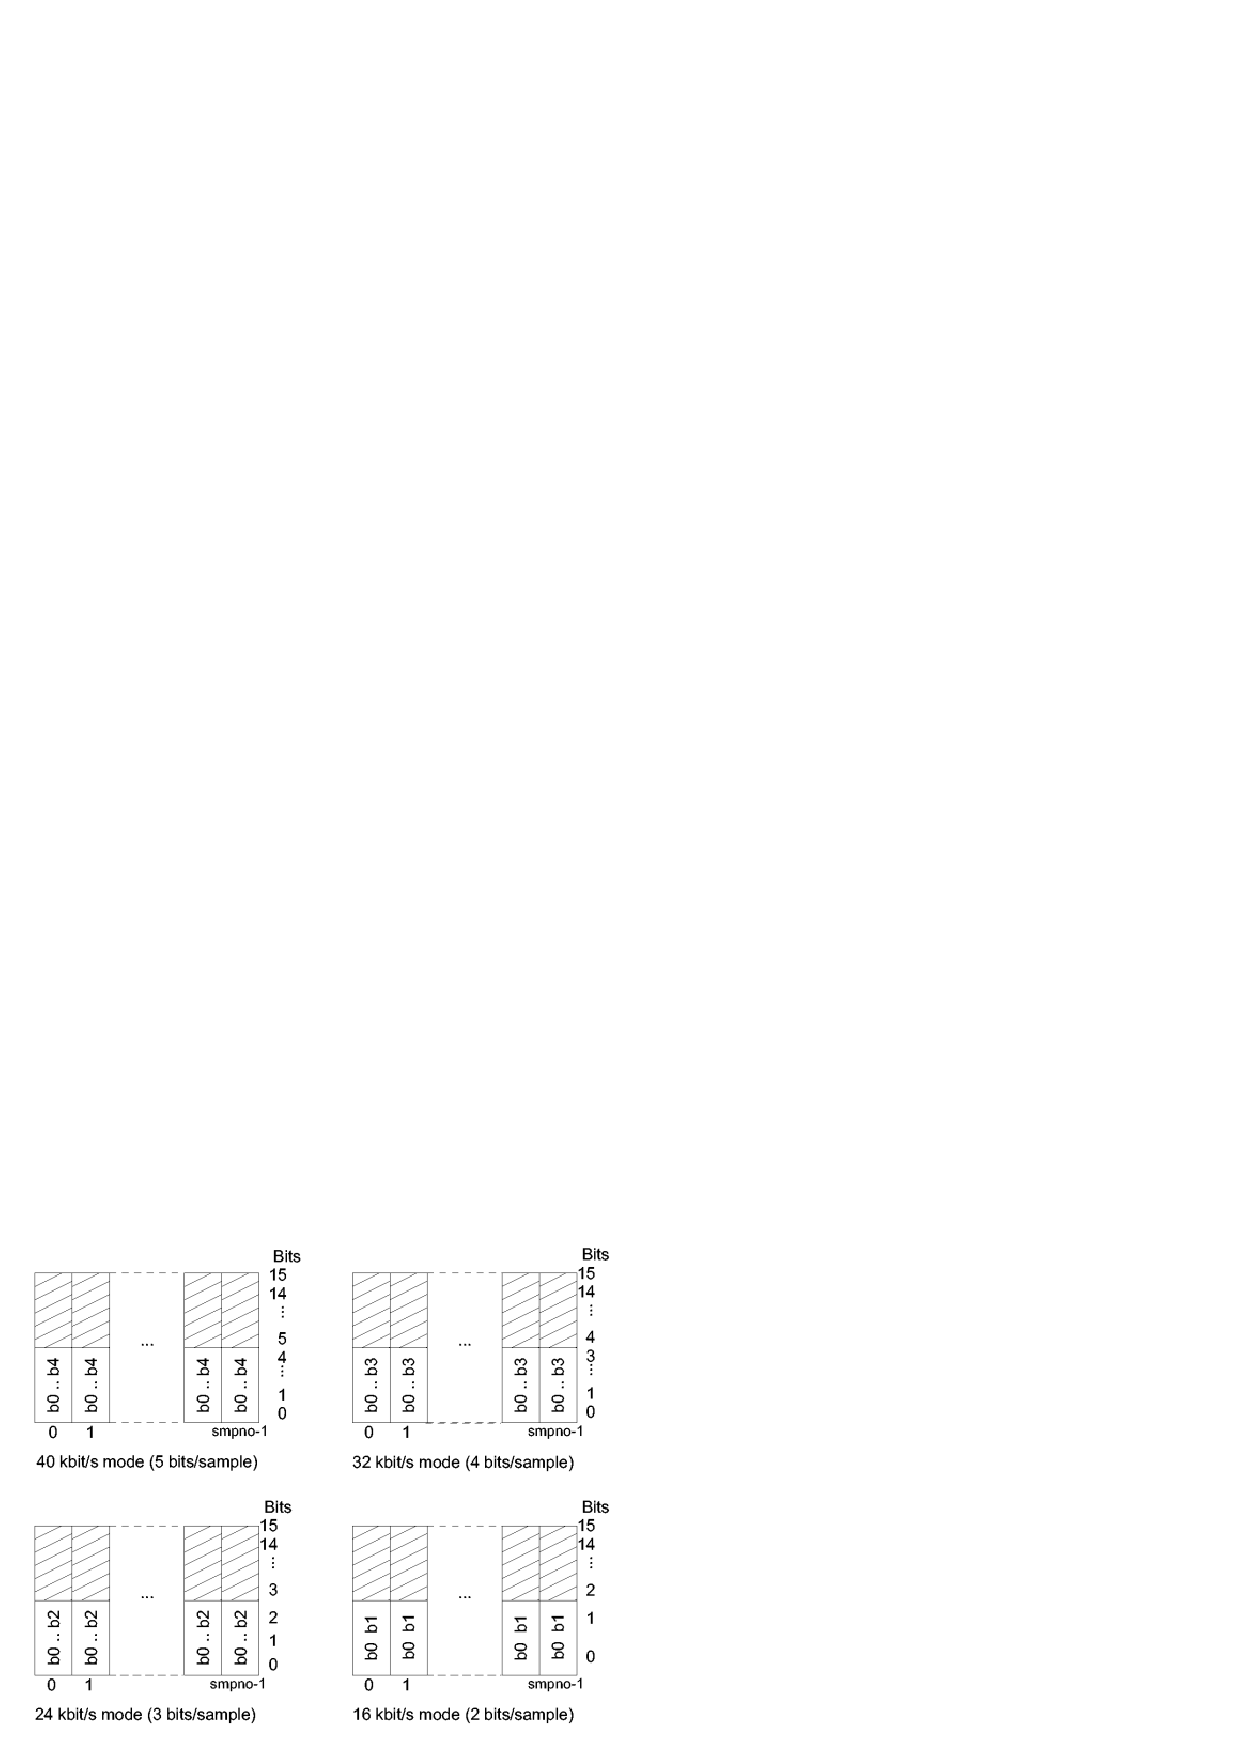
\includegraphics{bs-g726}
  \end{center}
  \caption{\SF Packing of G.726-encoded signals (right-aligned,
               parallel format).\label{G726-bs}}
\end{figure}
%------------------ End of IIR filter -----------------------------------

{\bf Prototype: }    g726.h

{\bf Description: }

        Simulation of the ITU-T G.726 ADPCM encoder. Takes the A or
        $\mu$ law input array of shorts {\em inp\_buf} (16 bit,
        right-justified, without sign extension) with {\em smpno}
        samples, and saves the encoded samples in the array of shorts
        {\em out\_buf}, with the same number of samples and
        right-justified. An example of the sample packing for the
        G.726 encoded bitstream is shown in figure \ref{G726-bs}.

        The state variables are saved in the structure {\em state}, and the
        reset can be stablished by making {\em reset} equal to 1. The law
        is A if {\em law}=={\tt '1'}, and mu law if {\em law}=={\tt
        '0'}.

{\bf Variables: }
\begin{Descr}{\DescrLen}
\item[\pbox{20mm}{\em inp\_buf}] %\rulex{1mm}\\
               Is the input samples' buffer; each {\tt short} sample
               shall contain right-justified 8-bit wide valid A or $\mu$
               law samples.

\item[\pbox{20mm}{\em out\_buf}] %\rulex{1mm}\\
               Is the output samples' buffer; each {\tt short} sample
               will contain right-justified 2-, 3-, 4-, or 5-bit wide G.726
               ADPCM samples, depending on the rate used.

\item[\pbox{20mm}{\em smpno}] %\rulex{1mm}\\
               Is the number of samples in inp\_buf.

\item[\pbox{20mm}{\em law}] %\rulex{1mm}\\
               Is a char indicating if the law for the input samples is A
               ({\tt '1'}) or $\mu$ ({\tt '0'}). See note below.

\item[\pbox{20mm}{\em rate}] %\rulex{1mm}\\
               Is a short indicating the number of bits per sample to used by
               the algorithm: 5, 4, 3, or 2.

\item[\pbox{20mm}{\em reset}] %\rulex{1mm}\\
               Is the reset flag (see note below):\\
               $\bullet$ {\em 1}: reset is to be applied in the variables;\\
               $\bullet$ {\em 0}: processing is carried out without
               setting state variables to the reset state. \\
               Please note that this should normally be
               done only in the first call to the routine in processing a
               sample stream.

\item[\pbox{20mm}{\em state}] %\rulex{1mm}\\
               The state variable structure; all the variables here are for
               internal use of the G.726 algorithm, and should not be
               changed by the user. Fields of this structure are described
               above.
\end{Descr}

{\bf Note:} \hfill \pbox{145mm}{
               Please note the difference between {\em reset} and {\em
               law}: {\em reset} must be either 1 (0x01) or 0 (0x00), not
               `1' (0x31) or `0' (0x30), while {\em law} is exactly
               the opposite.
             }\\

{\bf Return value: }        None.


\subsection{{\tt G726\_decode}}

{\bf Syntax: }

{\tt
\#include "g726.h"\\
void G726\_decode
         (\ttpbox{110mm}{
             short {\em *inp\_buf}, short {\em *out\_buf}, long {\em smpno},
             char  {\em *law}, short {\em rate}, short {\em reset},
             G726\_state {\em *state})
         }
}

{\bf Prototype: }    g726.h

{\bf Description: }

        Simulation of the ITU-T G.726 ADPCM decoder. Takes
        the ADPCM input array of shorts {\em inp\_buf} (16 bit, right-
        justified, without sign extension) of length {\em smpno}, and
        saves the decoded samples (A or $\mu$ law) in the array of
        shorts {\em out\_buf}, with the same number of samples and
        right-justified.

        The state variables are saved in the structure {\em state}, and the
        reset can be stablished by making {\em reset} equal to 1. The law
        is A if {\em law}=={\tt '1'}, and mu law if {\em law}=={\tt
        '0'}.

{\bf Variables: }
\begin{Descr}{\DescrLen}
\item[\pbox{20mm}{\em inp\_buf}] %\rulex{1mm}\\
               Is the input samples' buffer; each {\tt short} sample
               will contain right-justified 2-, 3-, 4-, or 5-bit wide
               G.726 ADPCM samples.

\item[\pbox{20mm}{\em out\_buf}] %\rulex{1mm}\\
               Is the output samples' buffer; each {\tt short} sample
               shall contain right-justified 8-bit wide valid A or $\mu$
               law samples.

\item[\pbox{20mm}{\em smpno}] %\rulex{1mm}\\
               Is the number of samples in inp\_buf.

\item[\pbox{20mm}{\em law}] %\rulex{1mm}\\
               Is a char indicating if the law for the input samples is A
               ({\tt '1'}) or $\mu$ ({\tt '0'}). See note below.

\item[\pbox{20mm}{\em rate}] %\rulex{1mm}\\
               Is a short indicating the number of bits per sample to used by
               the algorithm: 5, 4, 3, or 2.

\item[\pbox{20mm}{\em reset}] %\rulex{1mm}\\
               Is the reset flag (see note below):\\
               $\bullet$ {\em 1}: reset is to be applied in the variables;\\
               $\bullet$ {\em 0}: processing done without setting state
               variables to reset state. \\
               Please note that this should normally be
               done only in the first call to the routine in processing a
               sample stream.

\item[\pbox{20mm}{\em state}] %\rulex{1mm}\\
               The state variable structure; all the variables here are for
               internal use of the G.721 algorithm, and should not be
               changed by the user. Fields of this structure are described
               above.
\end{Descr}

{\bf Note:} \hfill \pbox{145mm}{
               Please note the difference between {\em reset} and {\em
               law}: {\em reset} must be either 1 (0x01) or 0 (0x00), not
               `1' (0x31) or `0' (0x30), while {\em law} is exactly
               the opposite.
             }\\

{\bf Return value: }        None.


%-.-.-.-.-.-.-.-.-.-.-.-.-.-.-.-.-.-.-.-.-.-.-.-.-.-.-.-.-.-.-.
\section{Portability and compliance} \label{G.726-Port}

Code testing has been done using the reset test sequences for 40, 32,
24, and 16 kbit/s provided in the G.726 test sequence diskettes
(available from the ITU sales department). Other tests were also done
with speech files for the 32 kbit/s mode, comparing with reference
implementations, most noticeably the one from AT\&T Bell Laboratories,
which is the original implementation. Both test approaches generated
100\% compatibility of this implementation with the G.726.
\footnote{\SF The problem with the A-law 40 kbit/s test vector
{\tt ri40fa.o} present in the STL96 has been solved in the STL2000.}

The portability of the STL G.726 encoding function has been tested by
feeding the routine with the reset test sequences of the G.726 test
sequences diskettes (available from the ITU Secretariat). As inputs,
a binary version of the files nrm.a, ovr.a, nrm.m, ovr.m have been
used for the 4 bit rates; the output of {\tt G726\_encoder } was then
compared with a binary version of the files rn$rr$fa.i, rv$rr$fa.i,
rn$rr$fm.i, rv$rr$fm.i, $rr=16,24,32,40$, accordingly for each input
sequence and rate. The encoding routine passed the test when no
differences in the bit streams were found.

The portability test of the decoding function was carried out by
feeding this routine with the pertinent test sequences of the G.726
Test Sequences Diskettes. As inputs, a binary version of the files
rn$rr$fa.i, rv$rr$fa.i, rn$rr$fa.i, rv$rr$fa.i, rn$rr$fm.i,
rv$rr$fm.i, rn$rr$fm.i, rv$rr$fm.i, and i$rr$ (twice: one for A and
another for $\mu$ law) have been used, $rr$ being 16, 24, 32, and 40.
The output of {\tt G726\_decoder } was then compared with a binary
version of the files rn$rr$fa.o, rv$rr$fa.o, rn$rr$fx.o, rv$rr$fx.o,
rn$rr$fm.o, rv$rr$fm.o, rn$rr$fc.o, rv$rr$fc.o, ri$rr$fa.o,
ri$rr$fm.o ($rr$ as above), respectively for each input sequences.
All test vectors were properly processed.

These routines have been tested in VAX/VMS with VAX-C and GNU-C, in the PC
with  Borland C v3.0 (16-bit mode) and GNU-C (32-bit mode). In the Unix
environment for Sun cc, acc, and gcc, and in HP for gcc.


\section{Example code}

%..........................................................................
\subsection {Description of the demonstration programs}

Two programs are provided as demonstration programs for the G.726 module,
g726demo.c and vbr-g726.c.

Program {\tt g726demo.c} accepts input files in either 16-bit,
right-justified A- or $\mu$-law format (as generated by g711demo.c)
and encodes and/or decodes using one of the G.726 bit rates (16, 24,
32, or 40 kbit/s). Linear PCM files are not accepted by the
program. Three operations are possible: logarithmic in, logarithmic
out ({\em lolo}) logarithmic in, ADPCM out ({\em load}), or ADPCM in,
logarithmic out ({\em adlo}).

Program {\tt vbr-g726.c} can perform the same functions as {\tt
g726demo.c}, however it is capable of two additional features. It can
perform in variable bit rate mode, which is switched at user-specified
frame sizes (i.e. number of samples), and it can operate from 16-bit
linear PCM input files. In the latter case, A-law is used to compand
the linear signal prior to G.726 encoding, since G.726 Annex A
\cite{G.726:LinearIO} is not yet implemented in the STL.

%..........................................................................
\subsection {Simple example}

The following C code gives an example of G.726 coding and decoding
using  as input speech previously encoded by either the A- or
$\mu$-law functions available in the STL. The output samples will be
encoded using the same law of the input signal.

{\tt\small
\begin{verbatim}
#include <stdio.h>
#include "ugstdemo.h"
#include "g726.h"

#define BLK_LEN 256

void main(argc, argv)
  int             argc;
  char           *argv[];
{
  G726_state      encoder_state, decoder_state;
  char            law[4];
  short           bitrate, reset;
  char            FileIn[180], FileOut[180];
  short           tmp_buf[BLK_LEN], inp_buf[BLK_LEN], out_buf[BLK_LEN];
  FILE           *Fi, *Fo;

  /* Get parameters for processing */
  GET_PAR_S(1, "_Law: ......................... ", law);
  GET_PAR_I(2, "_Bit-rate: .................... ", bitrate);
  GET_PAR_S(2, "_Input File: .................. ", FileIn);
  GET_PAR_S(3, "_Output File: ................. ", FileOut);

  /* Opening input and output LOG-PCM files */
  Fi = fopen(FileIn, RB);
  Fo = fopen(FileOut, WB);

 /* File processing */
  reset = 1;                    /* set reset flag as YES */
  while (fread(inp_buf, BLK_LEN, sizeof(short), Fi) == BLK_LEN)
  {
    /* Process input log PCM samples in blocks of length BLK_LEN */
    G726_encode(inp_buf, tmp_buf, BLK_LEN, law, bitrate, reset, &encoder_state);

    /* Process ADPCM samples in blocks of length BLK_LEN */
    G726_decode(tmp_buf, out_buf, BLK_LEN, law, bitrate, reset, &decoder_state);

    /* Write PCM output word */
    fwrite(out_buf, BLK_LEN, sizeof(short), Fo);

    if (reset)
      reset = 0;                /* set reset flag as NOMORE */
  }

  /* Close input and output files */
  fclose(Fi);
  fclose(Fo);
}
\end{verbatim}
}


%=============================================================================
% chapter G.727: The ITU-T embedded ADPCM algorithm
%=============================================================================
%=============================================================================
% ..... THIS IS chapter{G.727: The ITU-T embedded ADPCM algorithm } .....
% ... Revision:
% May.2000 - Convergence towards STL2000
% Nov.2000 - SG16 Plenary
% Feb.2001 - Edits in example section
%=============================================================================
\chapter{G.727: The ITU-T embedded ADPCM algorithm at
         40, 32, 24, and 16 kbit/s}
%=============================================================================



\section{Description of the Embedded ADPCM}

The G.727 algorithm is specified in Recommendation ITU-T G.727 \cite{G.727} with the block diagram shown in Figure \ref{fig:G.727}, and will not be further described here.
Additional information can be found in \cite{ADPCM-Tech-Report}, where a thorough comparison is made between different ADPCM schemes, including G.726 and G.727.
Details on the linear interface for the G.727 algorithm are found in G.727 Annex A \cite{G.727:LinearIO}.


\subsection{Extension for linear input and output signals}

An extension of the G.727 algorithm was carried out in 1994 to include, as
an option, linear input and output signals. The specification for such linear
interface is given in its Annex A \cite{G.727:LinearIO}.

This extension bypasses the PCM format conversion block for linear input
signals, and both the Output PCM Format Conversion and the Synchronous
Coding Adjustment blocks, for linear output signals. These linear versions
of the input and output signals are 14-bit, 2's complement samples.

The effect of removing the PCM encoding and decoding is to decrease the
coding degradation by 0.6 to 1 qdu, depending on the network configuration
considered (presence or absence of a G.712 filtering).

Currently, this extension has not been incorporated in the STL.

%-----------------------------------------------------
%Box dimension: 19.16cm x 20.74cm
\begin{figure}[hbtp]
  \begin{center}

   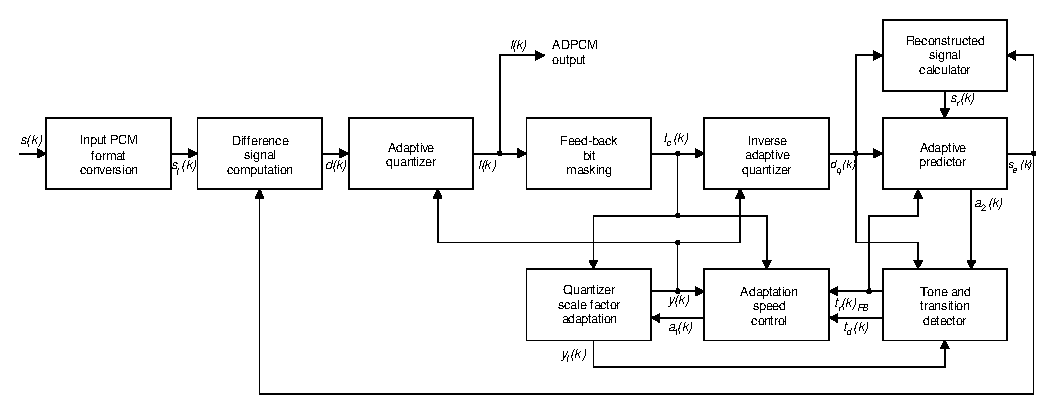
\includegraphics[scale=0.9]{g727-enc}\\

  (a) Encoder\\*[10mm]

  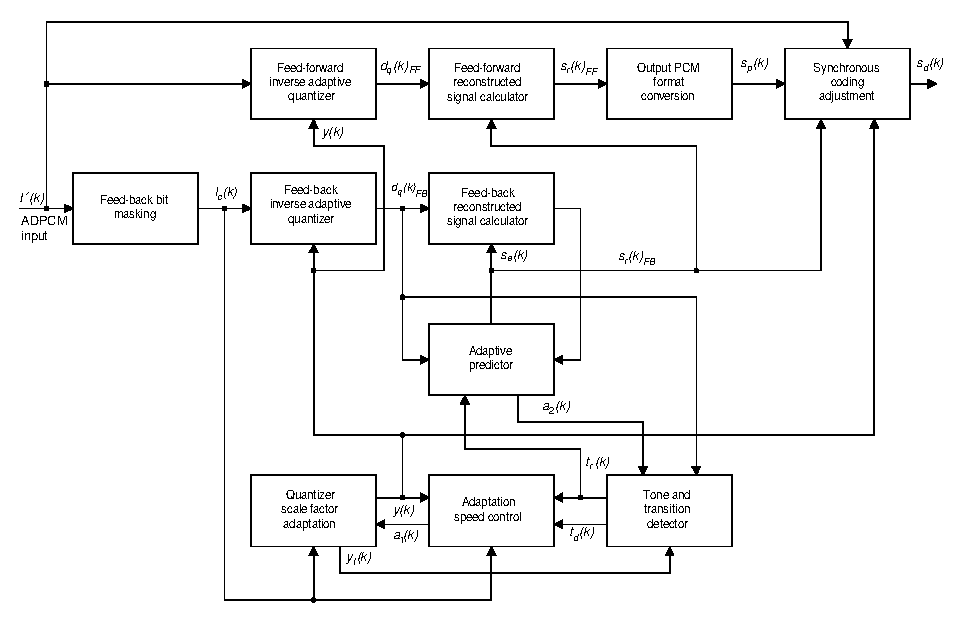
\includegraphics[scale=0.9]{g727-dec}\\

  (b) Decoder
  \end{center}

  \caption{G.727 encoder and decoder block diagrams
           \label{fig:G.727} }
\end{figure}
%-------------------------------------------------------------


\section{ITU-T STL G.727 Implementation}

The STL implementation of the G.727 algorithm can be found
in module {\tt g727.c}, with prototypes in {\tt g727.h}.

The problem of storing the state variables was solved by defining a
structure containing all the necessary variables, defining a new type
called {\tt G727\_state}. As for other STL modules, the use of the
state variable allows for parallel processing flows in the same
executable program. The internal elements of the state variable {\tt
G727\_state} should not be modified by the user, and are not described
here.

The encoding function is {\tt G727\_encode}, and the decoding function
is {\tt G727\_decode}. Additionally, initialization and reset of the
state variable is performed by {\tt g727\_reset}. There are other
internal routines which are not for access by the user, and hence are
not described here. Their usage description is given below.

\subsection{{\tt G727\_reset}}

{\bf Syntax: }

{\tt
\#include "g727.h"\\
void G727\_reset
         (\ttpbox{110mm}{
            g727\_state {\em *st});
         }
}

{\bf Prototype: }    g727.h

{\bf Description: }

  Reset ITU-T G.727 embedded ADPCM encoder or decoder state variable.


\subsection{{\tt G727\_encode}}

{\bf Syntax: }

{\tt
\#include "g727.h"\\
void G727\_encode
         (\ttpbox{110mm}{
                short {\em *src}, short {\em *dst}, short {\em smpno},
                short {\em law}, short {\em cbits}, short {\em ebits},
                g727\_state {\em *state});
         }
}

{\bf Prototype: }    g727.h

{\bf Description: }

Simulation of the ITU-T G.727 embedded ADPCM encoder. Takes the A or
$\mu$ law input array of shorts {\tt src} (16 bit, right- justified,
without sign extension) of length {\tt smpno}, and saves the encoded
samples in the array of shorts {\tt dst}, with the same number of
samples and right-justified. The ADPCM samples will have {\tt cbits}
core bits, and {\tt ebits} enhancement bits.

The state variables are saved in the structure {\em state}, which
should be initialized by {\tt g727\_reset()} before use. A-law is used
if {\em law}=={\tt '1'}, and $\mu$-law if {\em law}=={\tt '0'}.

{\bf Variables: }
\begin{Descr}{\DescrLen}
\item[\pbox{20mm}{\em src}] %\rulex{1mm}\\
               Is the input samples' buffer; each {\tt short} sample
               shall contain right-justified 8-bit wide valid A or $\mu$
               law samples.

\item[\pbox{20mm}{\em dst}] %\rulex{1mm}\\
               Buffer with right justified {\tt short} ADPCM-encoded
               samples with cbits core bits and ebits enhancement
               bits. Unused MSbs are set to zero.

\item[\pbox{20mm}{\em smpno}] %\rulex{1mm}\\
               Is a {\tt short} indicating the number of samples to encode.

\item[\pbox{20mm}{\em law}] %\rulex{1mm}\\
               Is a char indicating if the law for the input samples is A
               ({\tt '1'}) or $\mu$ ({\tt '0'}).

\item[\pbox{20mm}{\em cbits}] %\rulex{1mm}\\
               Number of core ADPCM bits.

\item[\pbox{20mm}{\em ebits}] %\rulex{1mm}\\
               Number of enhancement ADPCM bits.

\item[\pbox{20mm}{\em state}] %\rulex{1mm}\\
               The state variable structure; all the variables here are for
               internal use of the G.727 algorithm, and should not be
               changed by the user.
\end{Descr}

{\bf Return value: }        None.


\subsection{{\tt G727\_decode}}

{\bf Syntax: }

{\tt
\#include "g727.h"\\
void G727\_decode
         (\ttpbox{110mm}{
                short {\em *src}, short {\em *dst}, short {\em smpno},
                short {\em law}, short {\em cbits},
                short {\em ebits}, g727\_state {\em *state} );
         }
}

{\bf Prototype: }    g727.h

{\bf Description: }

Simulation of the ITU-T G.727 embedded ADPCM decoder. Takes the ADPCM
input array of shorts {\tt src} (16 bit, right-justified, without sign
extension) of length {\tt smpno}, and saves the decoded samples (A or
$\mu$ law) in the array of shorts {\tt dst}, with the same number of
samples and right-justified. The ADPCM samples must have {\tt cbits}
core bits, and {\tt ebits} enhancement bits.

The state variables are saved in structure {\tt st}, which should be
initialized by {\tt g727\_reset()} before use. The law is A if {\em
law}=={\tt '1'}, and $\mu$ law if {\em law}=={\tt '0'}.

{\bf Variables: }
\begin{Descr}{\DescrLen}
\item[\pbox{20mm}{\em src}] %\rulex{1mm}\\
               Buffer with right justified {\tt short} ADPCM-encoded
               samples with cbits core bits and ebits enhancement
               bits. Unused MSbs are zero.

\item[\pbox{20mm}{\em dst}] %\rulex{1mm}\\
               Is the input samples' buffer; each {\tt short} sample
               shall contain right-justified 8-bit wide valid A or $\mu$
               law samples.

\item[\pbox{20mm}{\em smpno}] %\rulex{1mm}\\
               Is a {\tt short} indicating the number of samples to encode.

\item[\pbox{20mm}{\em law}] %\rulex{1mm}\\
               Is a char indicating if the law for the input samples is A
               ({\tt '1'}) or $\mu$ ({\tt '0'}).

\item[\pbox{20mm}{\em cbits}] %\rulex{1mm}\\
               Number of core ADPCM bits.

\item[\pbox{20mm}{\em ebits}] %\rulex{1mm}\\
               Number of enhancement ADPCM bits.

\item[\pbox{20mm}{\em state}] %\rulex{1mm}\\
               The state variable structure; all the variables here are for
               internal use of the G.727 algorithm, and should not be
               changed by the user.
\end{Descr}


{\bf Return value: }        None.


%-.-.-.-.-.-.-.-.-.-.-.-.-.-.-.-.-.-.-.-.-.-.-.-.-.-.-.-.-.-.-.
\section{Portability and compliance} \label{G.727-Port}

Code testing has been done using the reset test sequences for 5, 4, 3,
and 2 bits with the valid combination of core and enhancement
bits. The reset test sequences can be acquired from the ITU Sales
Department, and are not distributed with the STL. The testing
procedure is implemented in the makefiles, which use a binary version
of the test vectors. The implementation passed the compliance test
when no differences were found between tested and reference test
vectors.  All test vectors were verified to be properly processed.

These routines have been tested in in MS-DOS with Turbo C++ v1.0
(16-bit mode) and GNU-C (go32 32-bit mode), and in Windows/32 with MS
Visual C and CYGNUS/gcc. In the Unix environment, they have been
tested for SunOs (cc, acc, and gcc), HP-UX (gcc), and Ultrix 4.0 (cc
and gcc).


\section{Example code}

%..........................................................................
\subsection {Description of the demonstration program}

One program is provided as demonstration program for the G.727 module,
g727demo.c.

Program {\tt g727demo.c} accepts input files in either 16-bit,
right-justified A- or $\mu$-law format (as generated by g711demo.c)
and encodes and/or decodes using the G.727 algorithm for the
user-specified number of $N_c$ core bits and $N_e$ enhancement
bits. The effective encoding bitrate will then be $16 \times
(N_c+N_e)$ kbit/s. Linear PCM files are not accepted by the program,
since G.727 Annex A \cite{G.727:LinearIO} is not yet implemented in
the STL. Three operations are possible: logarithmic in, logarithmic
out (default) logarithmic in, ADPCM out (option {\em -enc}), or ADPCM
in, logarithmic out (option {\em -dec}).

%..........................................................................
\subsection {Simple example}

The following C code gives an example of G.727 coding and decoding
using as input speech previously encoded by either the A- or
$\mu$-law functions available in the STL. The output samples are
encoded using the same law of the input signal.

{\tt\small
\begin{verbatim}
#include <stdio.h>
#include "ugstdemo.h"
#include "g727.h"

#define BLK_LEN 256

void main(argc, argv)
  int             argc;
  char           *argv[];
{
  G727_state      encoder_state, decoder_state;
  char            law;
  short           core, enh;
  char            FileIn[180], FileOut[180];
  short           tmp_buf[BLK_LEN], inp_buf[BLK_LEN], out_buf[BLK_LEN];
  FILE           *Fi, *Fo;

  /* Get parameters for processing */
  GET_PAR_C(1, "_Law: ......................... ", law);
  GET_PAR_I(2, "_Core bits: ................... ", core);
  GET_PAR_I(2, "_Enhancement bits: ............ ", enh);
  GET_PAR_S(2, "_Log-PCM Input File: .......... ", FileIn);
  GET_PAR_S(3, "_Log-PCM Output File: ......... ", FileOut);

  /* Opening input and output LOG-PCM files */
  Fi = fopen(FileIn, RB);
  Fo = fopen(FileOut, WB);

  /* Reset state variables */
  g727_reset(&encoder_state);
  g727_reset(&decoder_state);

  /* File processing */
  while (fread(inp_buf, BLK_LEN, sizeof(short), Fi) == BLK_LEN)
  {
    /* Process input log PCM samples in blocks of length BLK_LEN */
    G727_encode(inp_buf, tmp_buf, BLK_LEN, law, core, enh, &encoder_state);

    /* Process ADPCM samples in blocks of length BLK_LEN */
    G727_decode(tmp_buf, out_buf, BLK_LEN, law, core, enh, &decoder_state);

    /* Write PCM output word */
    fwrite(out_buf, BLK_LEN, sizeof(short), Fo);
  }

  /* Close input and output files */
  fclose(Fi);
  fclose(Fo);
}
\end{verbatim}
}


%%=============================================================================
% chapter G.728: ITU-T's low-delay CELP algorithm at 16 kbit/s
%=============================================================================
\include{g728}

%=============================================================================
% chapter G.722: The ITU-T 64 kbit/s wideband speech coding algorithm
%=============================================================================
%=============================================================================
% ..... THIS IS chapter{G.722: The ITU-T 64, 56, and 48 kbit/s wideband codec } .....
%  ... Revision:
% Oct.1995 - Created
% Jan.1996 - Peter Kroon revision
% Feb.2000 - Convergence towards STL2000
% Feb.2001 - Edits in example section
% Oct.2008 & august 2009 - Tool Update: introduction of G.192-compliant
%            bitstream basic operators and basic PLC options  -
%            Nicklas Sandgren, Jonas Svedberg, Balazs Kovesi, Adrien
%            Cormier, Claude Lamblin, Yusuke Hiwasaki
%=============================================================================
\chapter{G.722: The ITU-T 64, 56, and 48 kbit/s wideband
         speech coding algorithm}
%=============================================================================

With the emergence of ISDN networks offering digital connectivity at
64 kbit/s between subscribers, the possibility was given to improve
the standard telephone quality by increasing the transmitted
bandwidth. A bandwidth of 50-7000 Hz corresponding to a sampling of 16
kHz was chosen because it provides a substantial improvement of the
quality for applications where the speech is to be heard through
high quality loudspeakers e.g. for audio or video conference services,
commentary broadcasting, and high quality handsfree phones.

An expert group was created in November 1983 whose mandate was to
define a standard for 7 kHz speech coding within 64 kbit/s. After many
contributions received from several organisations, it has been decided
to choose a coder which combined subband filtering and adaptive
differential pulse-code modulation algorithms (SB-ADPCM). The final
recommendation was produced in March 1986 and approved in July 1986 by
the then CCITT SG XVIII as Recommendation \textcolor{blue}{ITU-T} G.722 \cite{G.722}.

The full description on the implementation of the G.722 algorithm is
found in \cite{G.722}, and network aspects related to its operation
are found in \cite{G.725}. Figure \ref{fig:G.722-systemic} summarizes
some systemic aspects of the G.722 algorithm. Overview and notes on
the development of the G.722 algorithm can be found in several papers
\cite{G.722:General,G.722:Overview,G.722:SubjTest,G.722:Implementation,
 G.722:Modes,G.722:Applications}.  The following description of the
G.722 algorithm is based on the text in \cite{G.722:Summary}.

In 2006, upon ETSI DECT request, packet loss concealment (PLC)
procedures for G.722 were standardized to ensure a sufficient
robustness over the DECT wireless interface. ITU-T G.722 at 64 kbit/s
codec is the mandatory coder in ETSI New Generation DECT (NG-DECT)
standards (ETSI TS 102 527-1 and -3)
\cite{G.722:ETSITS102527-1,G.722:ETSITS102527-3}. These standards are
intended for wideband audio enabled devices to be connected on VoIP
networks.
 
In the above mentioned PLC standardization, G.722 software tool was
updated. Originally, the ITU-T G.722 algorithm used its own binary bit
stream format without synchronism headers; this made almost impossible
to apply frame errors. In the STL 2009, G.722 codec software tool was
made compliant with G.192 bitstream format and EID-XOR/G.192 style of
frame and bit error application to G.722 is enabled. At the same time,
STL basic operators and complexity counters were
introduced. Furthermore, the standalone decoder tool now includes
basic reference Packet Loss Concealment functionality.

%-----------------------------------------------------
%Box dimension: 19.16cm x 20.74cm
\begin{figure}[hbtp]
    \begin{center}
        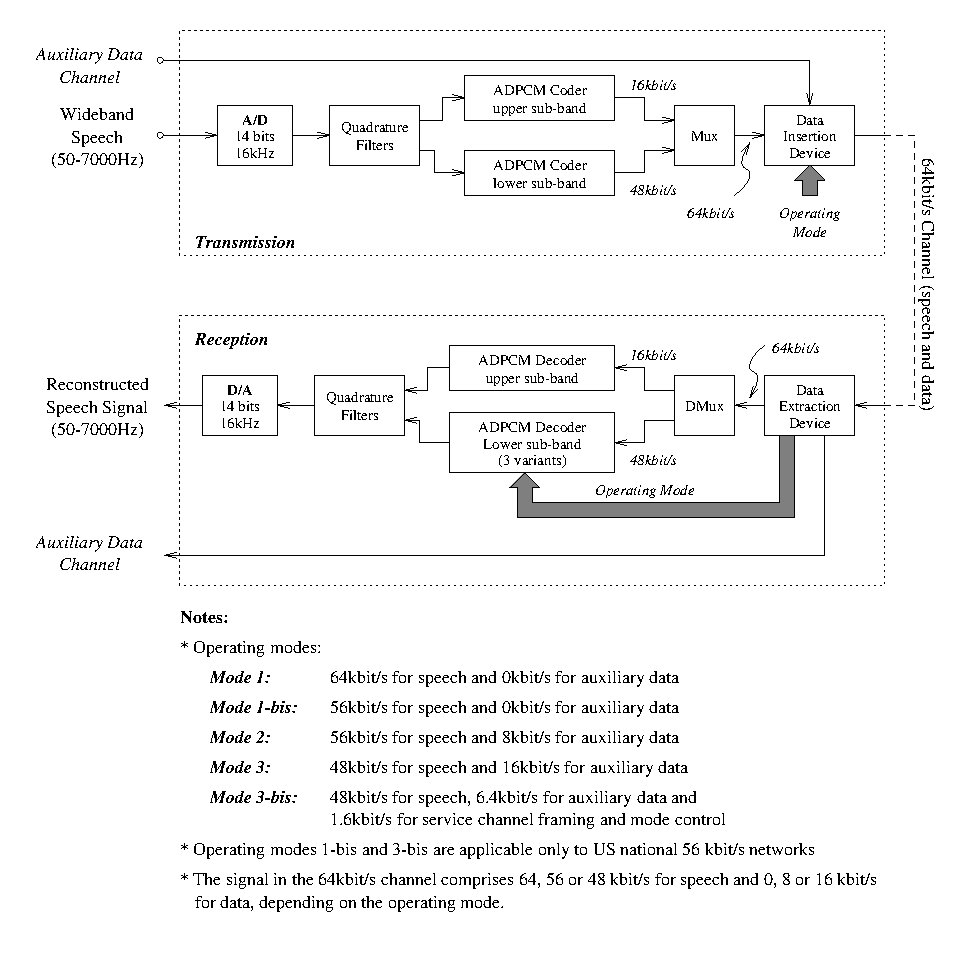
\includegraphics{g722}
  \end{center}
  \caption{G.722 encoder and decoder block diagrams
           \label{fig:G.722-systemic} }
\end{figure}
%-------------------------------------------------------------


%-----------------------------------------------------------------------------
\section{Description of the 64, 56, and 48 kbit/s G.722 algorithm}

In order to improve the transmitted speech quality, the input signal
has to be converted after antialiasing filtering by an
analog-to-digital (A/D) converter operating at 16 kHz sampling rate
and with a resolution of at least 14 uniform PCM bits. Similarly, at
the receive side, a digital-to-analog (D/A) converter operating at 16
kHz sampling rate and with a resolution of at least 14 uniform PCM
bits should be used. The specifications of the transmission
characteristics of the audio parts suited for the G.722 algorithm are
described in the Recommendation.  Some flexibility of the output bit
rate was implemented to allow the opening of an auxiliary data channel
within the 64 kbit/s channel.


%...............................................................
\subsection{Functional description of the SB-ADPCM encoder}\label{G722:descr-encoder}

Figure \ref{G722:encoder} shows block diagram of the SB-ADPCM encoder
which comprises the following main blocks.

%------------------------------
% G.722 Encoder
%------------------------------
\begin{figure}
    \begin{center}
    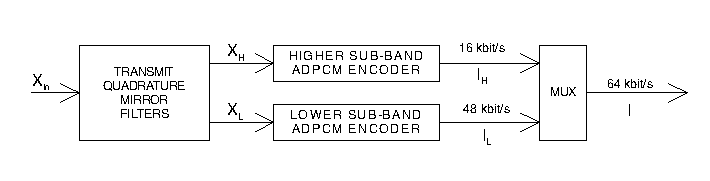
\includegraphics{g722-enc}
  \end{center}
  \caption{Block diagram of the SB-ADPCM encoder
           \label{G722:encoder}}
\end{figure}
%------------------------------

%-.-.-.-.-.-.-.-.-.-.-.-.-.-.-.-.-.-.-.-.-.-.-.-.-.-.-
\subsubsection{Transmit quadrature mirror filters}

The input signal $X_{in}$ is first filtered by two quadrature mirror
filters (QMF) which split the frequency band [0, 8000 Hz] into two equal
subbands. The outputs $X_{L}$ and $X_{H}$ of the lower and higher subbands are downsampled at 8 kHz by the filtering procedure.


%-.-.-.-.-.-.-.-.-.-.-.-.-.-.-.-.-.-.-.-.-.-.-.-.-.-.-
\subsubsection{Lower subband ADPCM encoder}

Figure \ref{G722:low-encoder} gives block diagram of the lower subband
ADPCM encoder. To transmit the lower band, the encoder was designed to
operate at 6, 5 or 4 bits per sample, corresponding to 48, 40 or 32
kbit/s, respectively. The ADPCM algorithm is very similar to the
embedded ADPCM algorithm of \textcolor{blue}{Recommendation ITU-T} G.727
\cite{G.727}. It is an embedded ADPCM with 4 core bits and 2
additional bits. The embedded property was introduced to prevent
degradation in speech quality when the encoder and the decoder operate
during short intervals in different modes.

%------------------------------
% G.722 lower subband encoder
%------------------------------
\begin{figure}
    \begin{center}
    \includegraphics{g722-len}
  \end{center}
  \caption{Block diagram of the lower subband ADPCM encoder
           \label{G722:low-encoder}}
\end{figure}
%------------------------------

\paragraph{Adaptive quantizer}

A 60-level non-uniform adaptive quantizer is used to quantize the
difference $e_L$ between the input signal $X_{L}$ and the estimated
signal $S_{L}$. The output of the quantizer $I_{L}$ is the ADPCM
codeword for the lower subband. The 4 forbidden output codewords were
primarily introduced to prevent the generation of all zero codes at
all modes, but have also later been used to recover the 8 kHz content
used by the coder.


\paragraph{Inverse adaptive quantizer}

In the feedback loop the two least significant bits of $I_{L}$ are deleted to produce a 4 bit signal $I_{Lt}$ which is used for the adaptation of the quantizer scale factor and applied to a 15-level inverse adaptive quantizer to produce the quantized difference signal $d_{Lt}$.


\paragraph{Quantizer adaptation}

In order to maintain a wide dynamic range and minimize complexity, the
quantizer scale factor adaptation is performed in the base 2
logarithmic domain. The log-to-linear conversion is accomplished using
a lookup table. There is no adaptation of the speed control parameter
as in 32 kbit/s ADPCM \cite{G.726} because the encoder is designed to
transmit more than voiceband data.


\paragraph{Adaptive predictor and reconstructed signal computation}

The adaptive predictor structure is similar to the one used for G.727
ADPCM standard: 2 poles and 6 zeroes. The two sets of coefficients
(one for the poles and  the other for the zeroes section) are updated
using a simplified gradient algorithm. Stability constraints are
applied to the poles in order to prevent possible unstable
conditions. However, no predictor reset is applied for some specifics
inputs conditions as it is done in G.726 algorithm. The
reconstructed signal $r_{Lt}$ is computed by adding the quantized
difference signal $d_{Lt}$ to the signal estimate $S_{L}$ produced by the
adaptive predictor. The use of a 4-bit operation instead of a 6-bit
operation in the feedback loops of the lower band ADPCM encoder and
decoder allows for the insertion of data in the two least
significant bits without causing mistracking in the decoder.


%-.-.-.-.-.-.-.-.-.-.-.-.-.-.-.-.-.-.-.-.-.-.-.-.-.-.-
\subsubsection{Higher subband ADPCM encoder}

Figure \ref{G722:high-encoder} shows block diagram of the higher
subband ADPCM encoder. This encoder is designed to operate at 2 bits
per sample, corresponding to a fixed bitrate of 16 kbit/s. The
encoder algorithm is very similar to the lower band one but with the
following main differences. The quantizer is a 4-level non-linear
adaptive quantizer. The higher subband ADPCM encoder is not embedded,
hence the inverse quantizer uses the 2 bits in the feedback loop.

%------------------------------
% G.722 higher subband encoder
%------------------------------
\begin{figure}
    \begin{center}
    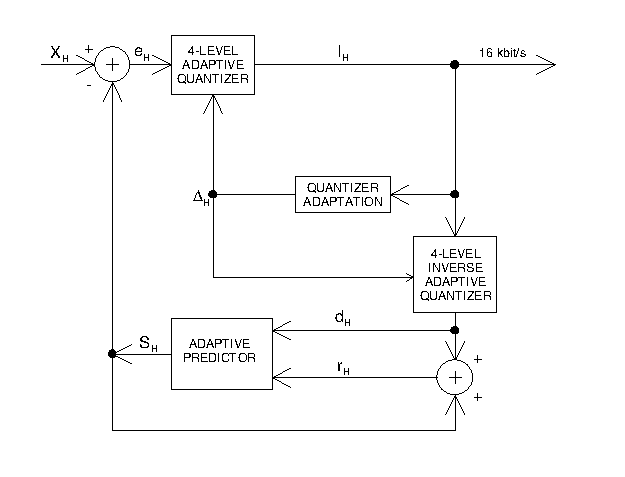
\includegraphics{g722-hen}
  \end{center}
  \caption{Block diagram of the higher subband ADPCM encoder
           \label{G722:high-encoder}}
\end{figure}
%------------------------------

%-.-.-.-.-.-.-.-.-.-.-.-.-.-.-.-.-.-.-.-.-.-.-.-.-.-.-
\subsubsection{Multiplexer}

The resulting codewords from the higher and lower subbands $I_H$ and
$I_L$ are combined to obtain the output codeword $I$ with an octet
format for transmission every 8 kHz frame resulting in 64~kbit/s. Note
that the 8 kHz clock may be provided by the network as it is always
done for 64 kbit/s A-law or $\mu$-law log-PCM (G.711) systems.


%...............................................................
\subsection{Functional description of the SB-ADPCM decoder}
            \label{G722:descr-decoder}

Figure \ref{G.722:decoder} shows block diagram of the SB-ADPCM decoder.


%-.-.-.-.-.-.-.-.-.-.-.-.-.-.-.-.-.-.-.-.-.-.-.-.-.-.-
\subsubsection{Demultiplexer}

The demultiplexer decomposes the received 64 kbit/s octet formatted
signal $I_r$ into two signals $I_{Lr}$ and $I_{Hr}$ which form the
codeword inputs for the lower and higher subband ADPCM decoders,
respectively.


%-.-.-.-.-.-.-.-.-.-.-.-.-.-.-.-.-.-.-.-.-.-.-.-.-.-.-
\subsubsection{Lower subband ADPCM decoder}

Figure \ref{G.722:low-decoder} shows a block diagram of the lower
subband decoder. This decoder operates in three different modes
depending on the received mode indication: 64, 56 and 48 kbit/s. The
block which produces the estimate signal is identical to the feedback
portion of the lower subband ADPCM encoder.  The reconstructed signal
$r_L$ is produced by adding the signal estimate to the relevant
quantized difference signals $d_{L,6}$, $d_{L,5}$ or $d_{L,4}$, which
are selected according to the received indication of the mode of
operation.


%-.-.-.-.-.-.-.-.-.-.-.-.-.-.-.-.-.-.-.-.-.-.-.-.-.-.-
\subsubsection{Higher subband ADPCM decoder}

This decoder (see Figure \ref{G.722:high-decoder}) is identical to the
feedback portion of the higher subband ADPCM encoder described in the
Section \ref{G722:descr-encoder}. Here, the output is reconstructed
signal $r_H$.

%------------------------------
% G.722 decoder
%------------------------------
\begin{figure}
    \begin{center}
        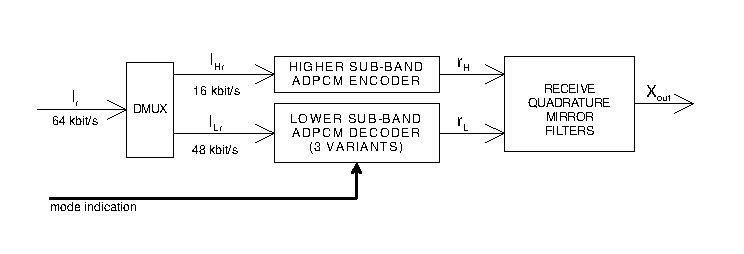
\includegraphics{g722-dec}
  \end{center}
  \caption{Block diagram of the SB-ADPCM decoder
           \label{G.722:decoder}}
\end{figure}
%------------------------------

%------------------------------
% G.722 lower subband decoder
%------------------------------
\begin{figure}
    \begin{center}
        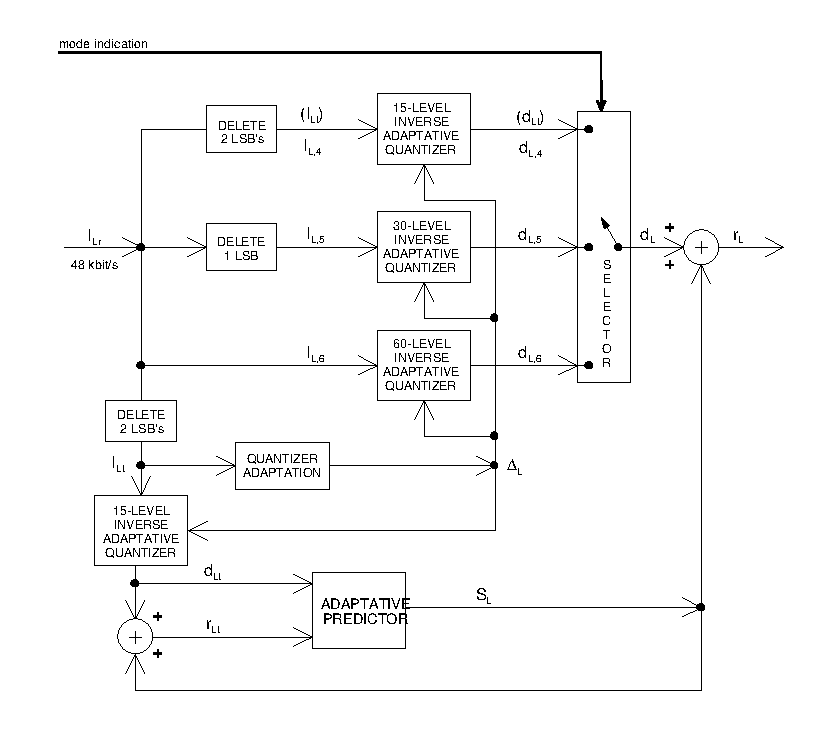
\includegraphics{g722-lde}
  \end{center}
  \caption{Block diagram of the lower subband ADPCM decoder
           \label{G.722:low-decoder}}
\end{figure}
%------------------------------

%------------------------------
% G.722 higher subband decoder
%------------------------------
\begin{figure}
    \begin{center}
        \includegraphics{g722-hde}
  \end{center}
  \caption{Block diagram of the higher subband ADPCM decoder
           \label{G.722:high-decoder}}
\end{figure}
%------------------------------

%-.-.-.-.-.-.-.-.-.-.-.-.-.-.-.-.-.-.-.-.-.-.-.-.-.-.-
\subsubsection{Receive QMF}

The receive QMF are two reconstruction filters which interpolate the
ouputs of the lower and higher subband ADPCM decoders from 8 to 16 kHz
($r_H$ and $r_L$) and generate 16~kHz sampling reconstructed output
$X_{out}$. Signal $X_{out}$ is converted to analog by the digital to
analog converter of the receiving side.

%...............................................................
\newpage

\subsection{Functional description of the basic Packet Loss Concealment functionality}

In 2006, basic index domain PLC functionality (zero index and frame
repeat algorithms) for detected frame errors were included in the
standalone decoder tool. The numbering and description of the four
basic algorithms provided can be seen in Table
\ref{tbl:G722StandaloneDecoder}.

\begin{table}[h]
  \begin{center}
  \begin{tabular}{|l|p{7cm}|}
	
\hline
PLC algorithm number & Description of concealment action \\
\hline
0 (default) & All bits in the erroneous frame are set to ``1''. (every 8 kHz octet index is set to 0xFF) \\
\hline
1	& same as PLC(0), but includes a decoder reset after the frame
decoding and synthesis operation.\\
\hline
2 & The bits from the previous frame(s) are repeated. After four erroneous frames, algorithm PLC(0) is used.  \\
\hline
3	& as PLC(2), but the first (0.625 ms) bits of the first good frame  after an erroneous frame are set to the value ``1''.  \\
\hline
  \end{tabular}
  \Caption{14cm}{\SF Basic PLC algorithms supported by the G.722 standalone decoder. \label{tbl:G722StandaloneDecoder}}
  \end{center}
\end{table}

The PLC actions in the G.722 standalone decoder are activated by
incoming G.192 frames that do not have a valid G192\_SYNC header
tag. Note that in November 2006, ITU-T SG16 approved two new
Appendices to G.722 for Packet Loss Concealment (PLC). These two
Appendices (Appendices III and IV \cite{G.722:AppIII,G.722:AppIV})
provide better quality over the basic PLC functionality included in
STL.

%-----------------------------------------------------------------------------
\section{Standalone G.192 compatible G.722 encoder and decoder tool}


\subsection{G.192 bit stream format for standalone G.722 encoder and decoder}

As described previously, G.722 is an embedded algorithm which supports
network scaling of the bitstream in three bitrates: 48, 56 and 64
kbit/s. To support this functionality within the G.192 file format the
G.722 encoder writes the 16 kbit/s embedded bits in the end of every
G.192 bitstream frame.
 
For every 16 kHz sample, there are eight G.722 encoded bits (an octet
index) to be transported in the G.192 frame. Bits b1 and b0 are the
embedded bits and bits b2-b7 are the non-embedded bits. In a G.192
frame, the b2 bits are written first in chunk, followed by that of b3,
until b7 bits. After all b7 bits are written, b1 bits are written and
then b0 bits. By sorting bits in this manner, truncation of a G.192
type G.722 frame bitstream from 64 kbit/s to 48 or 56 kbit/s is made
easy. Figures \ref{fig:G722trame}, \ref{fig:G722trame1} and
\ref{fig:G722trame2} show how the G.192 frames are composed for
various bit rates (64, 56, 48 kbit/s) and example frame sizes (10, 5,
20 ms). G.192 format is useful for enhanced simulation of G.722,
however actual application transport formats may be different (e.g. as
defined in \cite{G.722} and as used in \cite{G.722:RFC3551}).

\begin{figure}[h]
    \begin{center}
        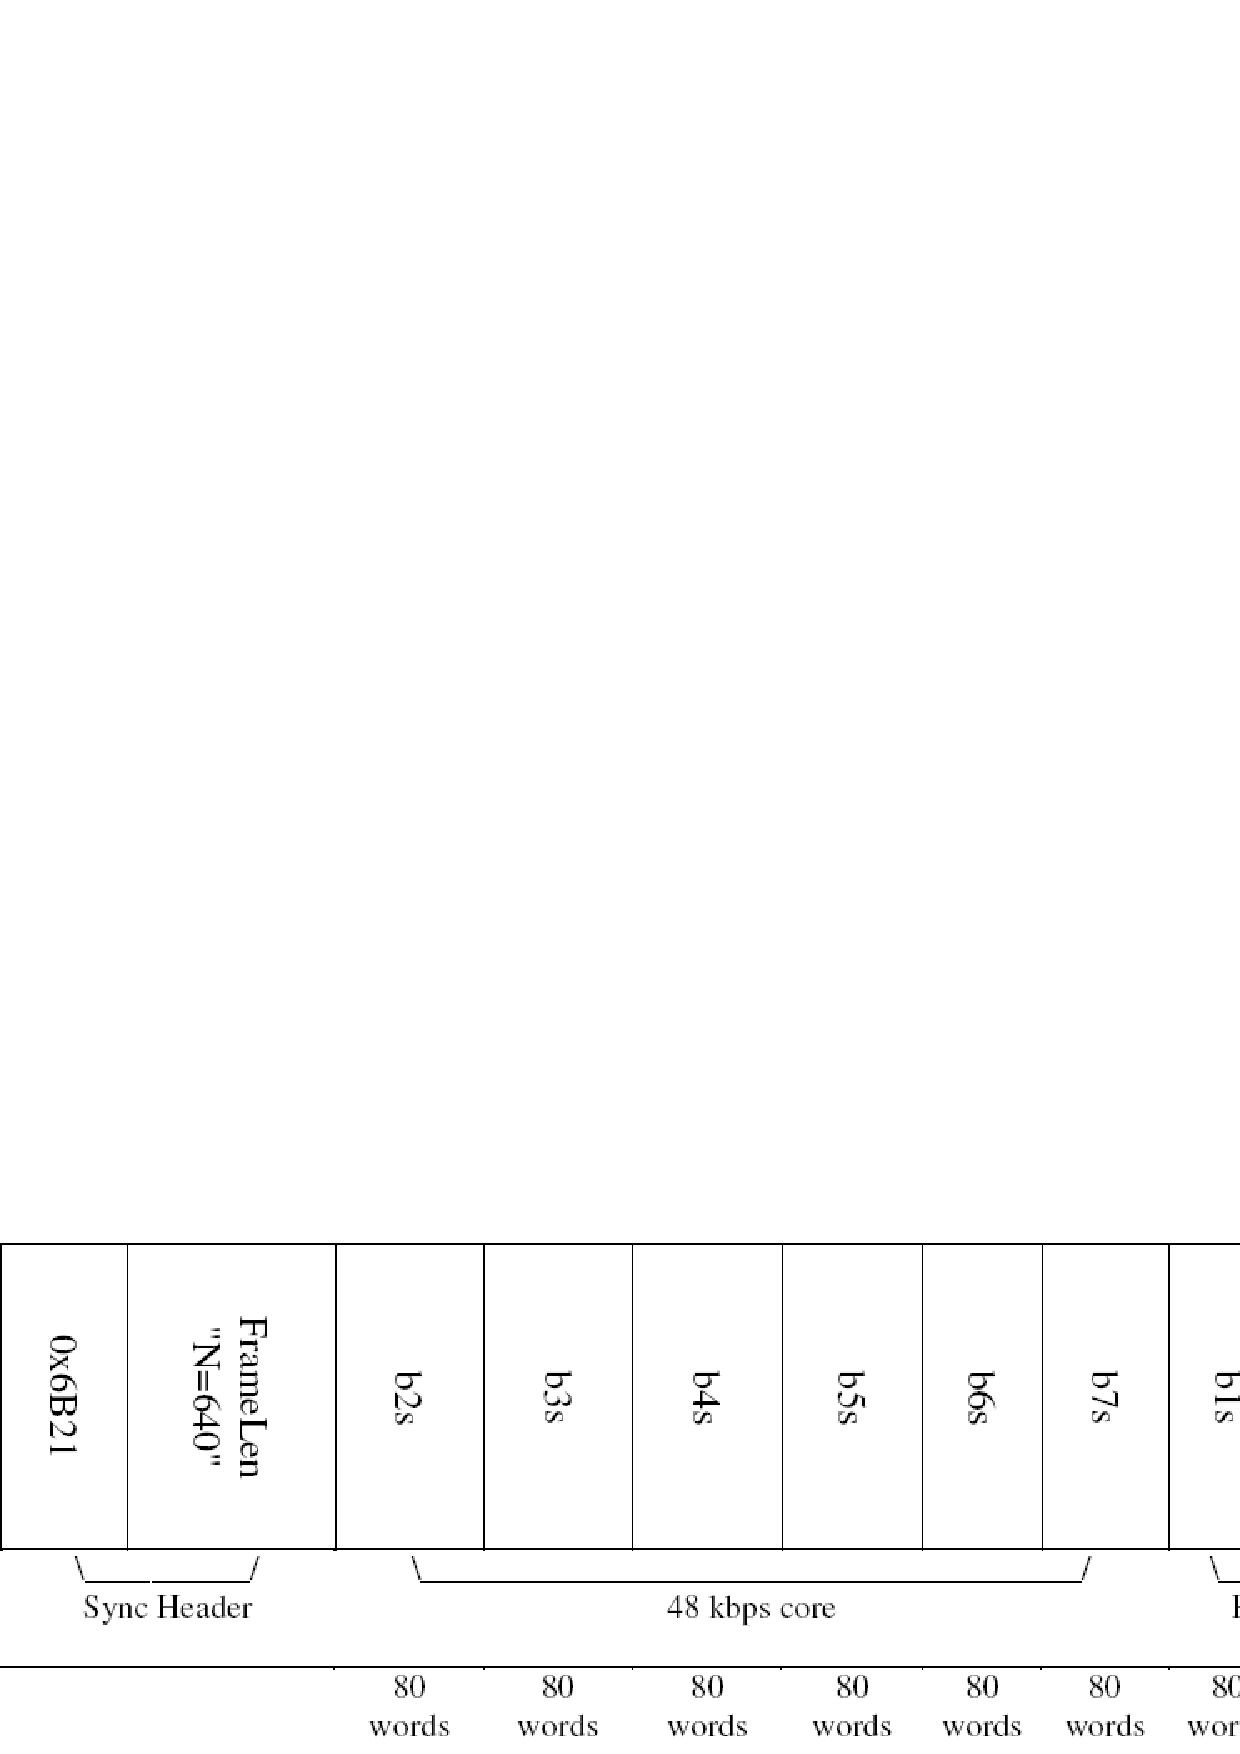
\includegraphics[scale=0.5]{G722trame}
  \end{center}
  \caption{Example of a G.192 compatible G.722 encoder output frame for a 10 ms input frame size. This frame has a length of 640 bits and a G192\_SYNC (0x6B21) header tag, in the G.192 file each g722 bit is stored as a 16 bit word.
           \label{fig:G722trame}}
\end{figure}

\pagebreak 

\begin{figure}[hbt]
    \begin{center}
      % \includegraphics[scale=0.5]{G722trame1}
        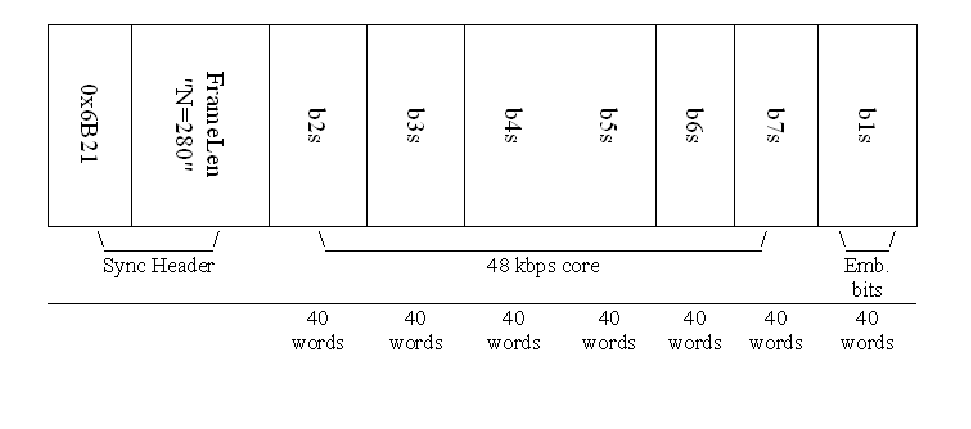
\includegraphics[scale=0.8]{G722trame1new}
%        \includegraphics[scale=0.5]{figure_g722_5ms_280bits.ps}
	    \caption{ Example of a G.192 compatible G.722 56 kbit/s encoder output frame for a 5 ms input frame size. This frame						has a length of 280 bits and a G192\_SYNC (0x6B21) header tag.
        \label{fig:G722trame1}}
	 \end{center}
\end{figure}

\begin{figure}[h]
    \begin{center}
        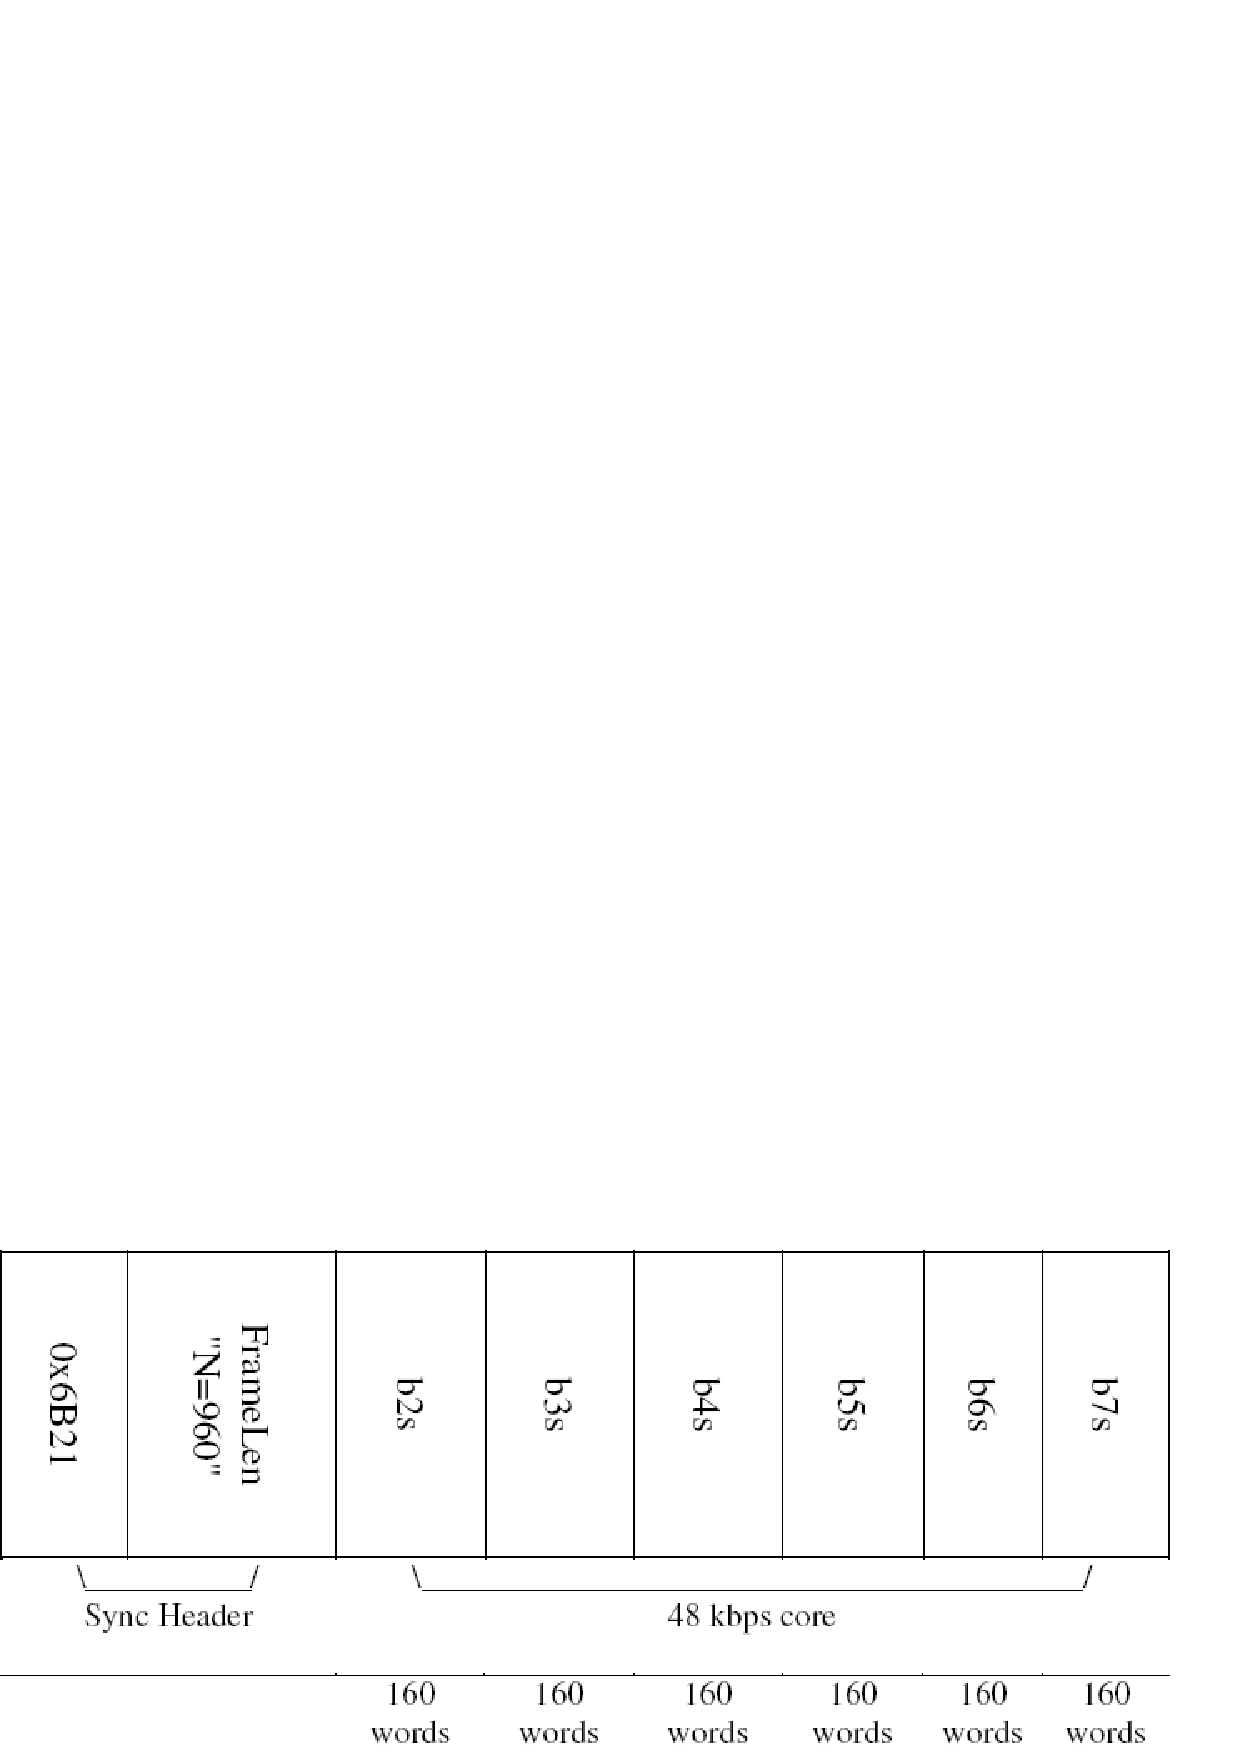
\includegraphics[scale=0.5]{G722trame2}
  \end{center}
  \caption{Example of G.192 compatible G.722 48 kbit/s encoder output frame for a 20 ms input frame size. This frame has a length of 960 bits and a G192\_SYNC (0x6B21) header tag.
           \label{fig:G722trame2}}
\end{figure}

\subsection{Standalone G.722 Encoder specific operation}

If the encoder can not read a complete input frame it stops its processing, this means that the final decoder output file may be up to a frame shorter than the input speech file. 

\pagebreak 

%-----------------------------------------------------------------------------
\section{ITU-T STL G.722 Implementation}

This implementation of the G.722 algorithm is composed of several
source files. The interface routines are in file {\tt g722.c}, with
prototypes in {\tt g722.h}. The original code of the STL G.722 was
provided by CNET/France and its user interface was modified to be
consistent with the other software modules of the STL. The update to
make G.722 tool compliant with G.192 bit stream format and include
basic PLC functionality was performed by Ericsson. The basic operators
and complexity counters were introduced by France Telecom.

The problem of storing the state variables was solved by defining a
structure called {\tt g722\_state} which containing all the necessary
state variables.  By means of this approach, several streams may be
processed in parallel\footnote{\SF This feature was not possible with
the original code provided by CNET and was added in the modifications
of the user interface.}, provided that one structure is assigned (and
that one call to the encoding/decoding routines is done) for each
data stream (this can be advantageous for machines with support for
parallel processing). The G.722 state structure has the following
fields (which are all {\tt shorts}):

\rulex{1pt} \hfill \begin{minipage}{150mm} \normalsize
 {\em ah, al} \hfill \pbox{120mm}{Second-order pole section coefficient
        buffer for higher and lower band, respectively}\\*[1mm]
 {\em bh, bl} \hfill \pbox{120mm}{Seventh-order zero section coefficient
        buffer for higher and lower band, respectively}\\*[1mm]
 {\em deth, detl} \hfill \pbox{120mm}{Delayed quantizer scale factor
        for higher and lower band, respectively}\\*[1mm]
 {\em dh} \hfill \pbox{120mm}{Quantizer difference signal memory}\\*[1mm]
 {\em dlt} \hfill \pbox{120mm}{Quantizer difference signal for the adaptive
        predictor}\\*[1mm]
 {\em init\_qmf\_rx} \hfill \pbox{120mm}{Flag indicating the need to
        initialize the QMF filters on the reception (decoder) side}\\*[1mm]
 {\em init\_qmf\_tx} \hfill \pbox{120mm}{Flag indicating the need to
        initialize the QMF filters on the transmission (encoder) side}\\*[1mm]
 {\em nbh, nbl} \hfill \pbox{120mm}{Delayed logarithmic quantizer factor
        for higher and lower band, respectively}\\*[1mm]
 {\em ph, plt} \hfill \pbox{120mm}{Partially reconstructed signal memory
        for higher and lower band, respectively}\\*[1mm]
 {\em qmf\_rx\_delayx} \hfill \pbox{120mm}{Memory of past 24 received (decoded)
        samples}\\*[1mm]
 {\em qmf\_tx\_delayx} \hfill \pbox{120mm}{Memory of past 24 transmitted
        (encoded) samples}\\*[1mm]
 {\em rh[3]} \hfill \pbox{120mm}{Quantized reconstructed signal}\\*[1mm]
 {\em rlt[3]} \hfill \pbox{120mm}{Reconstructed signal memory for the
        adaptive predictor}\\*[1mm]
 {\em sh, sl} \hfill \pbox{120mm}{Predictor output value for higher
        and lower band, respectively}\\*[1mm]
 {\em sph, spl} \hfill \pbox{120mm}{Pole section output signal for higher
        and lower band, respectively}\\*[1mm]
 {\em szh, szl} \hfill \pbox{120mm}{Zero section output signal for higher
        and lower band, respectively}\\
\end{minipage}

The default bitstream generated by the STL G.722 encoder is a G.192
compatible 16 bit output file and it is provided using the frame size
specified by the -fsize command. Bits in a G.192 bitstream frame are
ordered so that the frame can be truncated at 56 and 48 kbit/s. If the
number of input samples are non divisible by the frame size, the
output codeword stream is truncated at the last frame boundary.

A legacy g722 octet stream can be obtained using the option -byte.
The legacy bitstream generated by the STL G.722 encoder has 8 valid
bits for each encoded sample, saved in right-justified
{\short}s. i.e., the codewords are located in the lower 8-bits of the
encoded bitstream file. The MSB is always 0 for the 16 bit bitstream
file. The lower 6 bits are the lower-subband encoded bits, and the
upper two bits of the 8 valid bits are the upper-subband encoded
bits. When the decoder is not in operation mode 1, the decoder will
discard 1 or 2 of the lower bits of the lower-subband. It should be
noted that, when bit errors are inserted in this bitstream and the
operation mode is not mode 1, the actual bit error rate seen by the
decoder may not be the one actually desired. One may consider that, in
simulating a system where auxiliary data channels are used, such as
modes 2 and 3, this is actually the desired behaviour, because errors
hitting the auxiliary data will not affect the decoded speech
quality. However, if simulation of modes 1-bis or 3-bis is intended,
then the some of the errors hitting the lower 1 (mode 1-bis) or 2 bits
(mode 3-bis) will not be seen by the decoder, and the overall bit
error rate will actually be smaller than the desired one. There are
two possible approaches to circumvent this problem:
\begin{itemize}
 \item  the use of an external program to shift the bitstream samples
   one or two bits (respectively for modes 1-bis or 3-bis) to the right
   before the bitstream serialization process for use with the STL EID
   module, and an external program to left-shift
   the bitream samples by one or two bits after error insertion and
   before using the STL G.722 decoder. This solution is valid for both
   random and burst bit errors.
 \item  to increase proportionally the bit error rate by 1/8 (mode 1-bis) or
   1/4 (mode 3-bis), to statistically compensate for errors hitting unused 
   bits. This solution is valid only for random bit errors.
\end{itemize}

From the users' perspective, the encoding function is {\tt
g722\_encode}, and the decoding function is {\tt g722\_decode}.
Before using these functions, state variables for the encoder and the
decoder must be initialized respectively by {\tt g722\_reset\_encoder}
and {\tt g722\_reset\_decoder}. It should be noted that encoder and
decoder need individual state variables to work properly.

In the following part a summary of calls to the three entry functions
is found.

\subsection{{\tt g722\_encode}}

{\bf Syntax: }

{\tt
\#include "g722.h"\\
long g722\_encode (\ttpbox{110mm}{
            short {\em *inp\_buf},
            short {\em *g722\_frame},
            long  {\em smpno},
            g722\_state {\em *g722\_encode});
         }
}

{\bf Prototype: }    g722.h

{\bf Description: }

        Simulation of the ITU-T G.722 64 kbit/s encoder. Takes
        the linear (16-bit, left-justified) input array
        of shorts {\em inp\_buf} (16 bit,
        right-justified, without sign extension) with {\em smpno}
        samples, and saves the encoded bit-stream in the array of shorts
        {\em g722\_frame}. 

        The state variables are saved in the structure pointed by {\em
        g722\_encode}, and the reset can be established by making a
        call to {\tt g722\_reset\_encoder}.

{\bf Variables: }
\begin{Descr}{\DescrLen}
\item[\pbox{20mm}{\em inp\_buf}] %\rulex{1mm}\\
               Is the input samples' buffer with {\em smpno}
               left-justified 16-bit linear {\tt short} speech samples.

\item[\pbox{20mm}{\em g722\_frame}] %\rulex{1mm}\\
               Is the encoded samples' buffer; each {\tt short} sample
               will contain the encoded parameters as right-justified
               8-bit samples.

\item[\pbox{20mm}{\em smpno}] %\rulex{1mm}\\
               Is a long with the number of samples to be encoded from
               the input buffer {\em inp\_buf}.

\item[\pbox{20mm}{\em g722\_encode}] %\rulex{1mm}\\
               A pointer to the state variable structure; all the variables
               here are for
               internal use of the G.722 algorithm, and should not be
               changed by the user. Fields of this structure are described
               above.
\end{Descr}

        {\bf Return value: }

Returns the number of speech samples encoded.


\newpage
\subsection{{\tt g722\_decode}}

{\bf Syntax: }

{\tt
\#include "g722.h"\\
short g722\_decode (\ttpbox{110mm}{
            short {\em *g722\_frame},
            short {\em *out\_buf},
            int  {\em mode},
            long  {\em smpno},
            g722\_state {\em *g722\_decoder}, );
         }
}

{\bf Prototype: }    g722.h

\enlargethispage*{12mm}
{\bf Description: }

        Simulation of the ITU-T 64 kbit/s G.722 decoder. Reconstructs
        a linear (16-bit, left-justified) array
        of shorts {\em inp\_buf} (16 bit,
        right-justified, without sign extension) with {\em smpno}
        samples from the encoded bit-stream in the array of shorts
        {\em g722\_frame}. Include a basic Packet Loss Concealment functionality.

        The state variables are saved in the structure pointed by {\em
        g722\_decoder}, and the reset can be established by making a
        call to {\em g722\_reset\_decoder}.

{\bf Variables: }
\begin{Descr}{\DescrLen}
\item[\pbox{20mm}{\em g722\_frame}] %\rulex{1mm}\\
               Is the encoded samples' buffer; each {\tt short} sample
               will contain the encoded parameters as right-justified
               8-bit samples.

\item[\pbox{20mm}{\em out\_buf}] %\rulex{1mm}\\
               Is the output samples' buffer with {\em smpno}
               left-justified 16-bit linear {\tt short} speech samples.

\item[\pbox{20mm}{\em mode}] %\rulex{1mm}\\
               Is an {\tt int} which indicates the operation mode for the
               G.722 decoder. If equal to 1, the decoder will operate at
               64 kbit/s. If equal to 2, the decoder will operate at
               56 kbit/s, discarding the least significant bit of the
               lower-band ADPCM. If equal to 3, the decoder will
               discard the two least significant bits of the lower
               band ADPCM, being equivalent to the 48 kbit/s operation of
               the G.722 algorithm. It should be noted that, for this
               implementation of the G.722 algorithm, mode 1-bis is
               identical to mode 2, and mode 3-bis is identical to mode 3.

\item[\pbox{20mm}{\em smpno}] %\rulex{1mm}\\
               Is a long with the number of samples in the input
               encoded sample buffer {\em g722\_frame} to be decoded.

\item[\pbox{20mm}{\em g722\_decoder}] %\rulex{1mm}\\
               A pointer to the state variable structure; all the variables
               here are for
               internal use of the G.722 algorithm, and should not be
               changed by the user. Fields of this structure are described
               above.
\end{Descr}

        {\bf Return value: }

Returns the number of speech samples encoded.


\newpage
\subsection{{\tt g722\_reset\_encoder}}

{\bf Syntax: }

{\tt
\#include "g722.h"\\
     void g722\_reset\_encoder (g722\_state {\em *g722\_encoder});
}

{\bf Prototype: }    g722.h

{\bf Description: }

        Initializes the state variables for the G.722 encoder or decoder.
        Coder and decoder require each a different state variable.

{\bf Variables: }
\begin{Descr}{\DescrLen}
\item[\pbox{20mm}{\em g722\_encoder}] %\rulex{1mm}\\
        A pointer to the G.722 encoder state variable structure which
        is to be initialized.
\end{Descr}

{\bf Return value: }    None.


\subsection{{\tt g722\_reset\_decoder}}

{\bf Syntax: }

{\tt
\#include "g722.h"\\
  void g722\_reset\_decoder (g722\_state {\em *g722\_decoder});
}

{\bf Prototype: }    g722.h

{\bf Description: }

        Initializes the state variables for the G.722 decoder.
        Coder and decoder require each a different state variable.

{\bf Variables: }
\begin{Descr}{\DescrLen}
\item[\pbox{20mm}{\em g722\_decoder}] %\rulex{1mm}\\
        A pointer to the G.722 decoder state variable structure which
        is to be initialized.
\end{Descr}


{\bf Return value: }       None.

\newpage

%-----------------------------------------------------------------------------
\section{Portability and compliance}

The portability test for these routines has been performed using the
test sequences designed by the ITU-T for the G.722 algorithm\footnote{
  The G.722 test sequences are freely downloadable from
  http://www.itu.int/rec/T-REC-G.722-198703-I!AppII/en.}. It should be
noted that the G.722 test sequences are not designed to test the QMF
filters, but only to exercise the upper and lower band encoder and
decoder ADPCM algorithms. Therefore, testing of the codec with the
test sequences was done with a special set of test programs that used
the core G.722 upper- and lower-band ADPCM coding and decoding
functions. All test sequences were correctly processed.

This module has been compiled and tested on PC platform with Cygwin (CYGWIN\_NT-5.0), using gcc(3.3.3), and with Microsoft Visual Studio 8. 

Please note that the 16 bit oriented G.192 files require correct octet
swapping of inputs and outputs on big/little-endian machines.

%-----------------------------------------------------------------------------
\section{Encoder(encg722) tool command line options}

{\tt\small
\begin{verbatim}

Usage:
encg722  [-options] InpFile OutFile  
where:
InpFile     is the name of the speech file to be processed;
OutFile     is the name with the processed bitstream;

options:
-fsize  #   Number of 16 kHz input samples per frame (must be an even number).
            Default is 160 samples (16 kHz) (10 ms)  
-mode   #   Operating mode (1,2,3) (or rate 64, 56, 48 in kbit/s). 
            Default is mode 1 (= 64 kbit/s)
-frames #   number of frames to process
            (values -1 or 0 processes the whole file )
-byte       Provide encoder output data in legacy octet format.
            (default is g192). 			   
-h/-help    print help message


\end{verbatim}
}

%-----------------------------------------------------------------------------
\section{Decoder (decg722) tool command line options}
{\tt\small
\begin{verbatim}
Usage:

decg722 [-options] InpFile OutFile

where:
InpFile     is the name of the bit stream input file;
OutFile     is the name of the file with synthesized speech;

options:

-mode #     is the operation mode for the G.722 decoder.
            Default is mode 1/64 kbit/s.
            (others are mode 2/56 kbit/s and mode 3/48 kbit/s)

-fsize #    Number of samples per frame  
            Default is 160, 16 kHz samples (or 10ms)
            (NB! must be the same as on the encoder side.) 

-frames #   Number of frames to process

-plc #      Packet Loss Concealment algorithm number
            (0 = zero index insertion, no decoder state reset)
            (1 = zero index insertion, decoder state reset)
            (2 = previous frame repetition, no decoder state reset)
            (3 = previous frame repetition, a few zero_indeces in first good
             frame, no decoder state reset)
  
-byte       Use legacy nonG192 G.722 format (byte oriented) without
            frame/synch headers.

-h/-help    print help message
\end{verbatim}
}

%-----------------------------------------------------------------------------
\section{Example code}

%..........................................................................
\subsection {Description of the demonstration programs}

One demonstration program is provided for the G.722 module,
g722demo.c. In addition, two programs are provided in the distribution
when compliance testing of the encoder and decoder is necessary,
tstcg722.c and tstdg722.c\footnote{\SF. The demonstration program g722demo.c cannot be used for compliance verification because the test vectors for G.722 do not foresee processing through the quadrature mirror
filters.}. 

Program {\tt g722demo.c} accepts 16-bit, linear PCM samples sampled at
16 kHz as encoder input. The decoder also produces files in the same
format. The bitstream signals out of the encoder are always organized
in 16-bit, right-justified words that use the lower 8 bits (i.e., 64
kbit/s). According to the user-specified mode, the decoder will decode
the G.722-encoded bitstream using 64, 56, or 48 kbit/s (i.e. full 8
bits, discard 1 bit of the lower band, or discard 2 bits of the lower
band). 
It should be noted that the demonstration programs g722demo.c, tstcg722.c and tstdg722.c only produce G.722 legacy bitstream. To produce bitstream compliant with G.192, please use encg722.c and decg722.c. Similarly, basic PLC functionnality is not supported the demonstration programs g722demo.cand tstdg722.c. Please use decg722.c for basic PLC functionnality.

%..........................................................................
\subsection {Simple example}

The following C code gives an example of G.722 coding and decoding
using as input wideband speech which is encoded and decoded at either
64, 56, or 48 kbit/s, according to the user-specified parameter
{\em mode}.
{\tt\small
\begin{verbatim}
#include <stdio.h>
#include "ugstdemo.h"
#include "g722.h"
#define BLK_LEN 256

void main(argc, argv)
  int             argc;
  char           *argv[];
{
  g722_state      encoder_state, decoder_state;
  int             mode;
  char            FileIn[180], FileOut[180];
  short           smpno, tmp_buf[BLK_LEN], inp_buf[BLK_LEN], out_buf[BLK_LEN];
  FILE           *Fi, *Fo;

  /* Get parameters for processing */
  GET_PAR_S(1, "_Input File: .................. ", FileIn);
  GET_PAR_S(2, "_Output File: ................. ", FileOut);
  GET_PAR_I(3, "_Mode: ........................ ", mode);

  /* Initialize state structures */
  g722_reset_encoder(&encoder_state);
  g722_reset_decoder(&decoder_state);

  /* Opening input and output 16-bit linear PCM speech files */
  Fi = fopen(FileIn, RB);
  Fo = fopen(FileOut, WB);

 /* File processing */
  while (fread(inp_buf, BLK_LEN, sizeof(short), Fi) == BLK_LEN)
  {
    /* Encode input samples in blocks of length BLK_LEN */
    smpno = g722_encode(inp_buf, tmp_buf, BLK_LEN, &encoder_state);

    /* Decode G.722-coded samples in blocks of length BLK_LEN */
    smpno = g722_decode(tmp_buf, out_buf, mode, smpno, &decoder_state);

    /* Write 16-bit linear PCM output decoded samples */
    fwrite(out_buf, smpno, sizeof(short), Fo);
  }

  /* Close input and output files */
  fclose(Fi); fclose(Fo);
}
\end{verbatim}
}

%..........................................................................
\subsection {Example operation of encoder (encg722)}
{\tt\small
\begin{verbatim}
foreach mode ( 1 2 3 ) # (corresponds to 64,56,48 kbit/s)
   foreach fsize ( 160 320 640) # (corresponds to 10,20,40 ms) 
      encg722  -mode $mode -fsize $fsize inpsp.smp outp.g722.$fsize.$mode.g192 
   end #fsize 
end #mode
\end{verbatim}
}

%..........................................................................
\subsection {Example operation of decoder (decg722)}
{\tt\small
\begin{verbatim}
foreach mode ( 1 2 3 ) # (corresponds to 64,56,48 kbit/s)
   foreach fsize ( 160 320 640) # (corresponds to 10,20,40 ms) 
      decg722 -plc 0 -fsize $fsize outp.g722.$fsize.$mode.g192  outsp.smp
      mv outpsp.smp outpsp.g722.$fsize.$mode.plc.0.smp 
   end #fsize
end #mode
\end{verbatim}
}


%=============================================================================
% chapter RPE-LTP: GSM full-rate
%=============================================================================
%=============================================================================
% ..... THIS IS chapter{RPE-LTP: The full-rate GSM codec } .....
%  ... Revision:
% Nov.1995 - Created <Simao>
% Jan.1996 - Peter Kroon initial revision
% Jan.1996 - RPE description adapted from Peter Kroon's text
% Nov.1996 - William Navarro's comment on GSM history <simao>
% Feb.2000 - Convergence towards STL2000
% Nov.2000 - SG16 Plenary
% Feb.2001 - Edits in example section
%=============================================================================
\chapter{RPE-LTP: The full-rate GSM codec}
%=============================================================================

In 1988, the Groupe Special Mobile of the Conference Europe\'{e}ne
des Postes et Telecommunications (CEPT) approved the first
generation of a pan-European digital cellular radio system operating
at a net rate of 13 kbit/s\footnote{\SF The GSM standard developed
initially under the responsability of the CEPT was later transferred
to the European Standardisation Telecommunications Institute (ETSI),
and the acronym GSM had its meaning changed to Global System for
Mobile Communications. Currently, the GSM specifications are being
maintained by the Third Generation Partnership Project, 3GPP ({\tt
\url{www.3gpp.org}}).}. Its speech coding algorithm, the RPE-LTP
(Regular Pulse Excitation, Long Term Predictor) was a compromise
solution of the two best coders at that stage. The full-rate GSM
system started operation in the beginning of 1992 in some European
countries and its expansion is expected in a mid-term. This coder,
despite not being an ITU-T standard, is relevant for standardization
studies when scenarios involving tandeming conditions between the
PSTN and the European cellular system need to be studied.

The current version of the STL includes a RPE-LTP implementation
based on a  freely available implementation originally produced at
the Technical Institue of the University of Berlin, for a Unix
environment.  This code has been adapted, corrected to work on
several platforms, and tested with the recommended test vectors, all
properly processed.

Details on the algorithm can be found in several references
\cite{RPELTP:BasicConcept,RPELTP:ICASSP88,RPELTP:SpeechCommunication},
besides the Recommendation itself \cite{GSM-06.10}.


\section{Description of the 13 kbit/s RPE-LTP algorithm}
\label{principles}
The RPE-LTP is a frame based coder, encoding 20 ms frames of
input data at a time.
The encoder converts each 160 sample frame (8 kHz sampling rate,
13 bits uniform PCM format) into a bitstream frame of 260 bits.
The decoder uses the 260 bitstream bits to generate
a frame of 160 reconstructed speech samples.


\subsection{RPE-LTP Encoder}
A simplified block diagram of the RPE-LTP encoder \cite{GSM-06.10} is
shown in figure \ref{rpe-encoder}.

%--------------------------------------------------------
% RPE-LTP encoder
%--------------------------------------------------------
\begin{figure}
  \begin{center}
    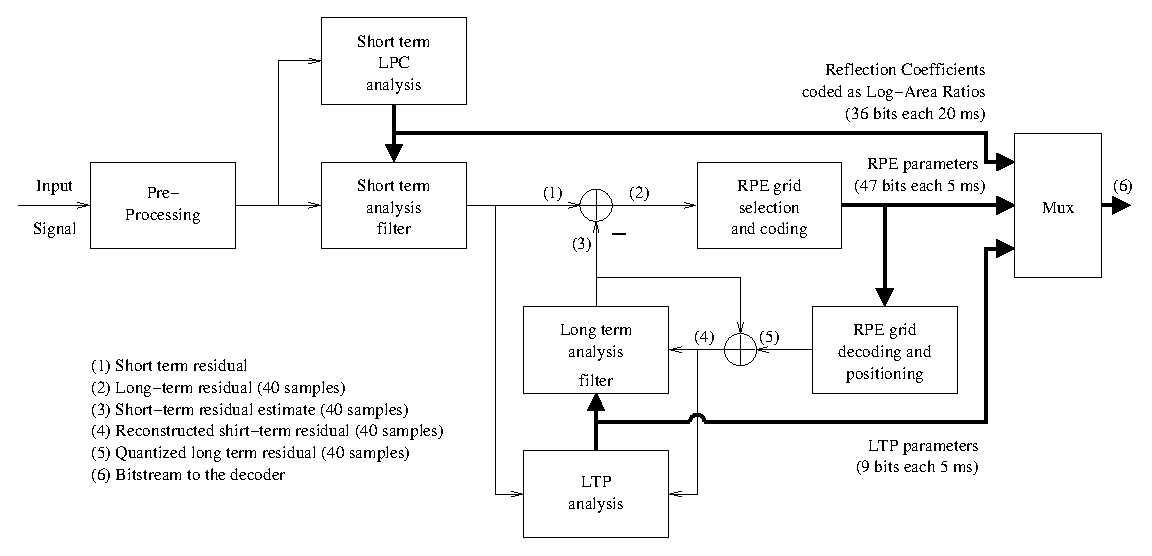
\includegraphics[width=15.5cm]{rpe-enc}
  \end{center}
%%  \begin{center}
%%    \makebox[10cm]{
%%      \rule{0cm}{17.22cm}
%%      \special{psfile=rpe-enc.ps hoffset=-297 voffset=-296 hscale=800 yscale=800}
%%    }
%%  \end{center}
  \caption{Simplified block diagram of the RPE-LTP encoder.
           \label{rpe-encoder}}
\end{figure}
%------------------------------------------------------------

The input speech frame, consisting of 160 uniform 13 bits PCM signal
samples, is first pre-processed to produce an offset-free signal, which
is then subjected to a first-order pre-emphasis filter. The 160
samples obtained are then analyzed to determine the coefficients for
the short-term analysis filter (LPC analysis). Using these coefficients
for the filtering of the same 160 samples produce the 160 samples of
the short-term residual signal. The filter parameters are represented
as reflection coefficients which are transformed to
log-area ratios (LARs) before transmission.

For the following operations, the speech frame is divided into 4
sub-blocks consisting each of 40 samples.
Before the processing of each sub-block, the parameters of the
long-term analysis filter, the LTP lag and the LTP gain, are estimated and
updated in the LTP analysis block. Estimation and update is performed
on the basis of the signal in the current sub-block and a stored
sequence of the 120 previously reconstructed short-term residual
samples.

A block of 40 long-term residual signal samples is obtained by
subtracting 40 estimates of the short-term residual from the
short-term residual signal itself. The resulting block is fed to the Regular
Pulse Excitation (RPE) analysis which performs the basic compression
function.

As a result of the RPE-analysis, the block of 40 input long-term
residual samples is represented by one of 4 candidate sub-sequences
of 13 pulses each. The subsequence selected is identified by the RPE
grid position. The 13 RPE pulses are encoded using Adaptive Pulse
Code Modulation (APCM) with estimation of the sub-block amplitude
which is transmitted to the decoder as side information. The RPE
parameters are also fed to a local RPE decoding and reconstruction
module which produces a block of 40 samples of the quantized version
of the long-term residual signal. By adding these 40 quantized
samples of the long-term residual to the previously obtained block of
short-term residual signal estimates, a reconstructed version of the
current short-term residual signal is obtained. The block of
reconstructed short-term residual signal samples is then fed to the
long-term analysis filter which produces the new block of 40
short-term residual signal estimates to be used for the next
sub-block thereby completing the feedback loop.

\subsection{RPE-LTP Decoder}

The simplified block diagram of the RPE-LTP decoder \cite{GSM-06.10}
is shown in figure \ref{rpe-decoder}.

%--------------------------------------------------------
% RPE-LTP encoder
%--------------------------------------------------------
%Box dimension: 21.17cm x 12.31cm
\begin{figure}
    \begin{center}
        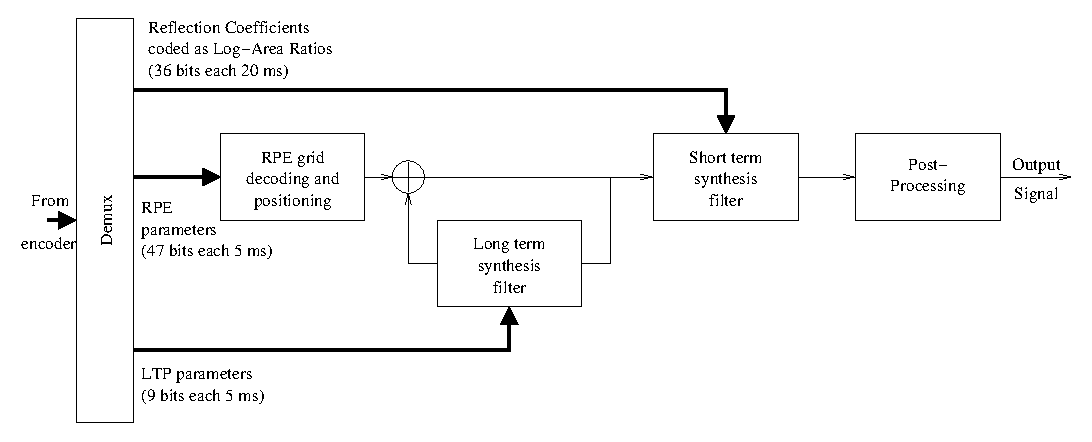
\includegraphics[width=15.5cm]{rpe-dec}
  \end{center}
%%  \begin{center}
%%    \makebox[10cm]{
%%      \rule{0cm}{12.31cm}
%%      \special{psfile=rpe-dec.ps hoffset=-300 voffset=-435}
%%    }
%%  \end{center}
  \caption{Simplified block diagram of the RPE-LTP decoder.
         \label{rpe-decoder}}
\end{figure}
%------------------------------------------------------------

The decoder includes the same structure as the feed-back loop of the
encoder. In error-free transmission, the output of this stage will be
the reconstructed short-term residual samples. These samples are then
applied to the short-term synthesis filter followed by the de-emphasis
filter resulting in the reconstructed speech signal samples.


\section{Implementation}

This implementation of the RPE-LTP algorithm is composed  of several
source files. The interface routines are in {\tt rpeltp.c},  with
prototypes in {\tt rpeltp.h}.

Originally written to be a device driver in Unix (known as {\em
toast}), its interface was adapted  to the specifications of the ITU-T
STL, and modified to operate correctly in a variety  of platforms,
like VAX, IBM PC compatibles, and Unix workstations (Sun and HP).

The problem of storing the state variables was solved by defining a
structure containing all the necessary variables, defining a new type
called {\tt gsm}, which is a pointer to a structure.  By means of
this approach, several streams may be processed in parallel, provided
that one structure is assigned (and that one call to the
encoding/decoding routines is done) for each data stream (this can be
advantageous for machines with support for parallel processing). The
RPE-LTP state structure has the following fields (all except {\em
L\_z2} and {\em mp}  are {\tt short}, which are {\tt long} and {\tt
int}, respectively):
\begin{quote} \normalsize
 {\em dp0} \hfill \pbox{120mm}{Memory of 280 past samples}
 {\em z1} \hfill \pbox{120mm}{DC-offset removal filter memory}
 {\em L\_z2} \hfill \pbox{120mm}{DC-offset removal filter parameter.}
 {\em mp} \hfill \pbox{120mm}{Preemphasis}
 {\em u} \hfill \pbox{120mm}{Eighth-order short term LPC analysis
        coefficients}
 {\em LARpp}\hfill \pbox{120mm}{Log Area Ratio array}
 {\em j}\hfill \pbox{120mm}{Index}
 {\em nrp} \hfill \pbox{120mm}{Long-term synthesis parameter}
 {\em v} \hfill \pbox{120mm}{Ninth order short-term synthesis vector}
 {\em msr} \hfill \pbox{120mm}{Post-processing parameter}
 {\em verbose} \hfill \pbox{120mm}{Flag used only if compiled
                                         with NDEBUG==0}
 {\em fast} \hfill \pbox{120mm}{Enables fast but inaccurate computation.
                                        Does not properly process the test
                                        sequences with this mode turned on.}
\end{quote}

Table \ref{RPE:bitstream} presents the RPE-LTP encoder output
parameters in order of occurence, with parameters defined in
\cite{GSM-06.10}. It should be noted that the bitstream file generated
by the STL implementation of the RPE-LTP algorithm uses an unpacked
format, as other codecs in the STL. Therefore, each of the 76
parameters indicated in table \ref{RPE:bitstream} occupy an unsigned,
right-adjusted 16-bit word. Unlikely to the G.711 and G.726
algorithms, however, the number of significant bits per bitstream
parameter is not the same for all the parameters, as can be seen from
the table. An important implication is that the STL bit error
insertion routines cannot be applied directly to the bitstream
generated by the STL RPE-LTP encoder. This limitation is not a
function of the EID module itself, but of the serialization and
parallelization (S/P) routines {\tt serialize\_*} and {\tt
parallize\_*} implemented in the Utility module, which are able only to
handle bitstreams that have the same number of valid bits per
sample. Solution to this problem still needs to be implemented in the
STL. It should be noted however that, since the full-rate GSM channel
coding is not implemented in the STL, bit error insertion directly in
the unprotected RPE-LTP bitstream will generally not be used. Should
the user need bit error insertion in the unprotected RPE-LTP
bitstream, there are two possible solutions:
\begin{itemize}
  \item it will be necessary to pack the bits for each parameter in
    such a way that, as seen by the S/P routines, each sample in the
    packed bitstream will have a constant number of valid bits per
    bitstream sample. Since there are 260 ($4 \times 5 \times 13$)
    bits for each frame, possible combinations are packed
    bitstreams with 65 16-bit words, of which the lower 4 bits are
    meaningful, or with 20 16-bit words, of which the lower 13 bits are
    meaningful. The former is preferred, despite the longer files
    generated.
  \item the user may modify the demonstration program to generate or accept
    (depending on whether it is an encoding or decoding operation) a
    serial bitstream format, as understood by the EID module, instead
    of a parallel bitstream format.
\end{itemize}

%--------------------------------------------------------------------------
% Table with description of the RPE-LTP bitstream
%--------------------------------------------------------------------------
\begin{table}
\centering\small
\caption{RPE-LTP bitstream format for each 20 ms speech frame.}
\begin{tabular}{|c|c|c|} \hline
\bf Parameter     & \bf Parameter & \bf Number \\
                  & \bf Number    & \bf of Bits\\
\hline
LAR1              &1    & 6 \\
LAR2              &2    & 6 \\
LAR3              &3    & 5 \\
LAR4              &4    & 5 \\
LAR5              &5    & 4 \\
LAR6              &6    & 4 \\
LAR7              &7    & 3 \\
LAR8              &8    & 3 \\
\hline
\multicolumn{3}{|c|}{\bf Sub-frame No. 1} \\
\hline
LTP lag           &9    & 7 \\
LTP gain          &10   & 2 \\
RPE grid position &11   & 2 \\
Block amplitude   &12   & 6 \\
RPE-pulse no. 1   &13   & 3 \\
$\ldots$          &$\ldots$ &$\ldots$\\
RPE-pulse no. 13  &25   & 3 \\
\hline
\multicolumn{3}{|c|}{\bf Sub-frame No. 2} \\
\hline
LTP lag           &26   & 7 \\
LTP gain          &27   & 2 \\
RPE grid position &28   & 2 \\
Block amplitude   &29   & 6 \\
RPE-pulse no. 1   &30   & 3 \\
$\ldots$          &$\ldots$ &$\ldots$\\
RPE-pulse no. 13  &42   & 3 \\
\hline
\multicolumn{3}{|c|}{\bf Sub-frame No. 3} \\
\hline
LTP lag           &43   & 7 \\
LTP gain          &44   & 2 \\
RPE grid position &45   & 2 \\
Block amplitude   &46   & 6 \\
RPE-pulse no. 1   &47   & 3 \\
$\ldots$          &$\ldots$ &$\ldots$\\
RPE-pulse no. 13  &59   & 3 \\
\hline
\multicolumn{3}{|c|}{\bf Sub-frame No. 4} \\
\hline
LTP lag           &60   & 7 \\
LTP gain          &61   & 2 \\
RPE grid position &62   & 2 \\
Block amplitude   &63   & 6 \\
RPE-pulse no. 1   &64   & 3 \\
$\ldots$          &$\ldots$ &$\ldots$\\
RPE-pulse no. 13  &76   & 3 \\
\hline
\end{tabular}
\label{RPE:bitstream}
\end{table}

From the users' perspective, the encoding function is {\tt
rpeltp\_encode}, and the decoding function is {\tt rpeltp\_decode}.
Before using these functions, the state variable for either the
encoder or the decoder must be initialized by {\tt rpeltp\_init}. It
should be noted that encoder and decoder need individual state
variables to work properly. After all the processing is performed, the
memory allocated for the state variables can be freed by calling {\tt
rpeltp\_delete}. The following sub-sections describe these four entry
functions for the STL RPE-LTP module.

\subsection{{\tt rpeltp\_encode}} \label{sec:rpeencode}

{\bf Syntax: }

{\tt
\#include "rpeltp.h"\\
void rpeltp\_encode (\ttpbox{110mm}{
            gsm {\em rpe\_state}, short {\em *inp\_buf},
            short {\em *rpe\_frame});
         }
}

{\bf Prototype: }    rpeltp.h

{\bf Description: }

        Simulation of the GSM full-rate RPE-LTP encoder. The 16-bit,
        left-justified linear-PCM input array of \short samples {\em
        inp\_buf} are processed by the RPE-LTP encoder and the encoded
        bit-stream is returned in the right-justified array of \short
        samples {\em rpe\_frame}, with one sample for each encoded
        parameter. The input frame has 160 samples and the encoded
        frame has 76 samples.

        The state variables are saved in the structure pointed by {\em
        rpe\_state}, previously initialized by a call to {\tt
        rpeltp\_init()}. The reset can be stablished by making a call
        to {\tt rpeltp\_init()}.

{\bf Variables: }
\begin{Descr}{\DescrLen}
\item[\pbox{20mm}{\em rpe\_state}] %\rulex{1mm}\\
               A pointer to the state variable structure. All the
               variables here are for internal use of the RPE-LTP
               algorithm and should not be changed by the
               user. Fields of this structure are described above.

\item[\pbox{20mm}{\em inp\_buf}] %\rulex{1mm}\\
               Is the linear-PCM input sample buffer which must have 160
               left-justified 16-bit linear-PCM \short samples. Only
               the 13 MSb are used.

\item[\pbox{20mm}{\em rpe\_frame}] %\rulex{1mm}\\
               Is the encoded sample buffer. Each \short sample will
               contain the encoded parameters as right-justified
               samples. The actual number of significant bits per
               sample will depend on each parameter.
\end{Descr}

        {\bf Return value: }        None.


\subsection{{\tt rpeltp\_decode}} \label{sec:rpedecode}

{\bf Syntax: }

{\tt
\#include "rpeltp.h"\\
void rpeltp\_decode (\ttpbox{110mm}{
            gsm {\em rpe\_state}, short {\em *rpe\_frame},
            short {\em *out\_buf});
         }
}

{\bf Prototype: }    rpeltp.h

{\bf Description: }

        Simulation of the GSM full-rate RPE-LTP decoder. The encoded
        bit-stream in the input array of right-justified \short
        samples {\em rpe\_frame} is used to reconstruct a block of the
        speech signal using the RPE-LTP decoder. The reconstructed
        speech block is returned in the 16-bit, left-justified
        linear-PCM output array of \short samples {\em inp\_buf}. The
        input frame has 76 samples and the decoded frame has 160
        samples.

        The state variables are saved in the structure pointed by {\em
        rpe\_state}, previously initialized by a call to {\tt
        rpeltp\_init()}. The reset can be established by calling {\tt
        rpeltp\_init()}.

{\bf Variables: }
\begin{Descr}{\DescrLen}
\item[\pbox{20mm}{\em rpe\_state}] %\rulex{1mm}\\
               A pointer to the state variable structure. All the
               variables here are for internal use of the RPE-LTP
               algorithm and should not be changed by the user. Fields
               of this structure are described above.

\item[\pbox{20mm}{\em rpe\_frame}] %\rulex{1mm}\\
               Is the encoded sample buffer, which must have 76
               right-justified \short samples. The actual number of
               bits per sample will depend on each parameter.

\item[\pbox{20mm}{\em out\_buf}] %\rulex{1mm}\\
               Is the output samples buffer, which will contain 160
               left-justified, 13-bit linear-PCM \short samples. The
               three LSbs are set to zero.
\end{Descr}

        {\bf Return value: }        None.

\subsection{{\tt rpeltp\_init}}

{\bf Syntax: }

{\tt
\#include "rpeltp.h"\\
gsm rpeltp\_init (void);
}

{\bf Prototype: }    rpeltp.h

{\bf Description: }

        Initializes the state variables for the RPE-LTP encoder or decoder.
        Combined coder and decoder operation requires a different state
        variable for the encoding and the decodeing part.

{\bf Variables: } None.

{\bf Return value: }

A pointer to an initialized state variable structure defined by the type
{\tt gsm}. Returns NULL in case of failure.

\subsection{{\tt rpeltp\_delete}}

{\bf Syntax: }

{\tt
\#include "rpeltp.h"\\
void rpeltp\_init (gsm rpe\_state);
}

{\bf Prototype: }    rpeltp.h

{\bf Description: }

Releases memory allocated to a state variable previously
initialized by rpeltp\_init().

{\bf Variables: }
\begin{Descr}{\DescrLen}
\item[\pbox{20mm}{\em rpe\_state}] %\rulex{1mm}\\
        A pointer to a previously initialized RPE-LTP state variable
        structure.
\end{Descr}

{\bf Return value: }

None.


\section{Portability and compliance}

The portability test for these routines has been done using
the test sequences designed by the GSM for the RPE-LTP
(available from ETSI), which were also used to verify the compliance of
the encoding and decoding function to the full-rate GSM voice codec
Recommendation \cite[Annex C]{GSM-06.10}.

This routine has been tested in VAX/VMS with VAX-C and gcc, in the PC
with Borland C v3.0 (16-bit mode) and gcc (32-bit mode). In the Unix
environment in a Sun workstation with cc, acc, and gcc, and in HP with
gcc. In all tested cases, 100\% of the test sequences passed when the
following symbols were defined at compilation time: {\tt SASR}, {\tt
USE\_FLOAT\_MUL} and {\tt NDEBUG}. The symbol {\em FAST} must not be
defined for perfomance compliant with the GSM 06.10 Recommendation,
while {\tt USE\_FLOAT\_MUL} {\bf must} be defined at compilation
time. The symbol {\tt NeedFunctionPrototypes} must be undefined for
pre-ANSI-C compilers (e.g. SunOS cc compiler).


%-----------------------------------------------------------------
\section{Example code}

%.................................................................
\subsection {Description of the demonstration program}

One program is provided as demonstration program for the RPE-LTP module,
rpedemo.c.

Program {\tt rpedemo.c} accepts input files in either 16-bit linear
PCM format, 16-bit, right-justified A-law format, or 16-bit,
right-justified $\mu$-law format for the encoding operation. The
output of the decoder can also be in any of these formats, but it will
have the same format as the encoding operation if encoding and
decoding is performed in a single pass (default). If the encoding and
decoding operations are performed in separate steps, the format of the
output signal does not need to match the format of the original linear
PCM signal.  The encoder output and decoder input are signals in
16-bit, right-justified samples, as described before in Sections
\ref{sec:rpeencode} and \ref{sec:rpedecode}. Three operations are
possible: encode and decode in a single pass (default), encode-only
(option {\em -enc}), or decode-only (option {\em -dec}).

%..........................................................................
\subsection {Simple example}

The following C code gives an example of RPE-LTP coding and decoding
using as input 13-bit, linear-PCM speech samples, which are encoded
and decoded at 13 kbit/s.

{\tt\small
\begin{verbatim}
#include <stdio.h>
#include "ugstdemo.h"
#include "rpeltp.h"

#define BLK_LEN 160

int main(argc, argv)
  int       argc;
  char     *argv[];
{
  gsm       encoder_state, decoder_state;

  char      FileIn[180], FileOut[180];
  short     bs_buf[BLK_LEN], inp_buf[BLK_LEN], out_buf[BLK_LEN];
  FILE     *Fi, *Fo;

  /* Get parameters for processing */
  GET_PAR_S(1, "_Input File: .................. ", FileIn);
  GET_PAR_S(2, "_Output File: ................. ", FileOut);

  /* Initialize state structures */
  encoder_state = rpeltp_init();
  decoder_state = rpeltp_init();

  /* Opening input and output LOG-PCM files */
  Fi = fopen(FileIn, RB);
  Fo = fopen(FileOut, WB);

 /* File processing */
  reset = 1;                    /* set reset flag as YES */
  while (fread(inp_buf, BLK_LEN, sizeof(short), Fi) == BLK_LEN)
  {
    /* Encode input linear PCM samples */
    rpeltp_encode(encoder_state, inp_buf, bs_buf, BLK_LEN);

    /* Decode samples */
    rpeltp_decode(decoder_state, bs_buf, out_buf);

    /* Write decoded samples */
    fwrite(out_buf, BLK_LEN, sizeof(short), Fo);

    if (reset)
      reset = 0;                /* set reset flag as NOMORE */
  }

  /* Free memory */
  rpe_delete(decoder_state);
  rpe_delete(encoder_state);

  /* Close input and output files */
  fclose(Fi);
  fclose(Fo);
  return 0;
}
\end{verbatim}
}


%=============================================================================
% chapter: RATE-CHANGE: Up and Down sampling module
%=============================================================================
%============================================================================%
% THIS IS ..... chapter{RATE-CHANGE: Up- and down-sampling module } .....     %
%============================================================================%
% Revision
% Jan.1995 - Simao Campos
% Nov.1995 - Simao Campos
% Jan.1996 - Peter Kroon, Simao Campos, Paul Voros
% Feb.1996 - Rafi Rabipour
% Apr.1996 - Mark Perkins, Simao Campos
% Feb.2000 - Convergence towards STL2000
% Nov.2000 - SG16 Plenary
% Feb.2001 - Edits in example section
% Apr.2005 - STL2005 revision -- Cyril Guillaum� & Stephane Smith
% Nov 2009 - STL2009 revision -- Adrien Cormier, Claude Lamblin and Yusuke Hiwasaki
%=============================================================================
\chapter{RATE-CHANGE: Up- and down-sampling module}
%=============================================================================

In certain applications involving digitized speech, such as
subjective evaluation of speech processed by digital algorithms, it
may be preferable to use sampling higher than the typical rate used
for the algorithms under test. This is desirable because simpler
analog filters with less phase distortion can be built. Another
advantage is that upper frequency components of the signal are not
lost. It also allows for the convenient shaping of the input signal,
such as IRS, $\Delta_{SM}$, and psophometric weightings.
Consequently there is a need to adapt the sampling rate of the
digitized signal to that of the processing algorithm.  For telephony
applications, the typical sampling rate is 8000 Hz with a signal
bandwidth in general of 300-3400 Hz, and for wideband speech
applications, a bandwidth of 50-7000 Hz is desired with sampling
rate of 16000 Hz. During the 2005-2008 ITU-T study period, greater audio bandwidth
were considered and superwideband and fullband audio codecs were developed. 
Their typical samplings rates are respectively 32000 Hz with a signal bandwidth 
of 50-14000 Hz, and 48000 Hz with a signal bandwidth of 20-20000 Hz.
Therefore, sampling rates above 8000 Hz and 16000
Hz are desirable, respectively. In several experiments
\cite{LDCELP-voitests} the sampling rate was 16 kHz. In others (see
\cite{ETSI-half} and \cite{AC-05-16}), 48 kHz and 32 kHz were
utilized. Hence the need for a software tool to carry out filtering
and sampling rate change. Next, the rate change and spectral
weighting routines implemented in the ITU-T STL are presented.


%-------------------------------------------
\section{Description of the Algorithm}

Signal processing theory describes the basic arrangement for
decimation of signals; first the signal is low-pass filtered to
limit its bandwidth in order to avoid aliasing when the rate is
lowered and, second, to decimate the samples, i.e., to drop out
samples from the input signal, such that the desired output rate is
obtained. For example, if a rate reduction from 48 kHz to 8
kHz is desired, a decimation factor of 6:1 is necessary. This is
equivalent to say that, after limiting the bandwidth of the digitized
speech to 4 kHz, 5 out 6 samples are skipped, or alternatively, only 1
out of 6 samples will be kept (or saved) from the signal.

The up-sampling of signals requires that each of the input samples be
followed by a number of zero samples, such that the desired output
rate is achieved; after this, an interpolation operation of these zero
samples is performed to obtain a continuous-envelope signal. For
example, up-sampling data from 8 kHz to 16 kHz requires interleaving
each sample of the input signal with a zero sample followed by
interpolation of the signal. This interpolation can be carried out by
means of a polynomial, which is equivalent to a filtering operation.

The type of filtering required is determined by the application
intended for the signals. For the tools needed in this version of the
STL, three different groups of characteristics were defined:

\rulex{5mm}
\begin{minipage}{150mm}
 $\bullet$ \parbox[t]{140mm}{
               {\bf High-quality}: Change in rate without changing the
               frequency response of the input signal. This is
               accomplished with a flat, linear phase, low-pass or bandpass
               FIR filter.}\\*[5mm]
 $\bullet$ \parbox[t]{140mm}{
               {\bf Spectral weighting}: Spectral weighting without
               rate change is necessary for some applications. For
               narrow-band speech, available are the IRS weighting
               specified in ITU-T Rec.  P.48, the so-called ``modified''
               IRS (annex D of ITU-T Rec.  P.830), the
               far-to-near-field conversion $\Delta_{SM}$ weighting,
               and the psophometric noise weighting of ITU-T
               Rec. O.41. For wideband signals, the mask for wideband
               handsets, as defined in ITU-T Rec. P.341, is also
               available. For super-wideband signals, the mask for
               super-wideband videoconferencing terminals
                has been derived as an extension of ITU-T Rec. P.341.}\\*[5mm]
 $\bullet$ \parbox[t]{140mm}{
               {\bf PCM quality}: Change in rate accompanied with
               modification of the frequency response of
               the input signal according to the mask specified
               in \textcolor{blue}{Recommendation ITU-T} G.712. This is accomplished
               with a non-linear phase low-pass IIR filter.}\\
\end{minipage}


%........................
\subsection{High-quality}

The response of the filters in this type of rate change must minimize
phase and amplitude distortion. For example, for decimation from 48
kHz to 16 kHz, the filter must be flat up to about 8 kHz (except for
the transition, or cut-off, region), with a linear phase. In other
cases, it may be desirable to remove the DC component and hum noise
(50--60 Hz AC line noise) from the signal without additional
phase distortion to the upper region of the spectrum.

%------------------ Begin of FIR filter --------------------------------
% this was x-y scaled by a factor of 6/7 (~0.85), to fit %
% and the box reduced in y by 1.26cm, to save space, and the ps data
% moved down by ~1cm (18 points)
\begin{figure}[hb]
  \begin{center}
    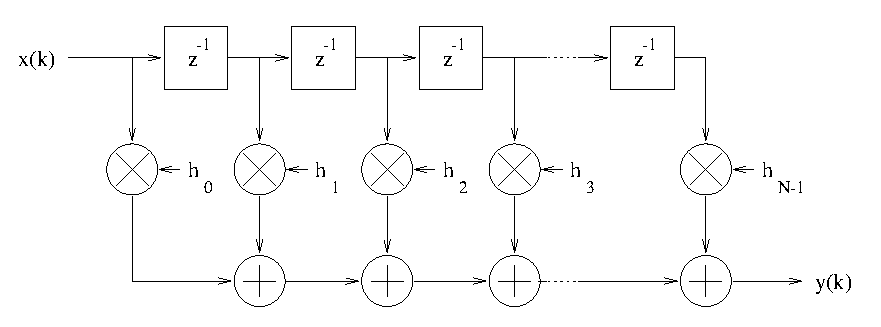
\includegraphics{fir}
  \end{center}
  \caption{\SF FIR filter block diagram.\label{FIR-filter}}
\end{figure}
%------------------ End of FIR filter -----------------------------------

One way to do this is to use a linear phase finite impulse
response (FIR) digital filter, as in figure \ref{FIR-filter}. The
input and output characteristic is defined by:
\[
      y(k) = \sum_{i=0}^{N-1} h(i) \cdot x(k-i)
\]
Linear phase is guaranteed if the filter is symmetric, i.e.:
\[
     h(k)=h(N-1-k), \mbox{ for } k=0..N-1
\]

%.........................
\subsection{Narrowband weighting}

\subsubsection{IRS weighting}

The IRS weighting corresponds to a bandpass filtering characteristic
whose mask can be found in \textcolor{blue}{Recommendation ITU-T} P.48 \cite{P.48}.
The send and receive spectral shapes of the IRS weighting were
obtained in a round-robin series of measurements made on a number of
analog telephones in the early 1970's
\cite{BNR-ModIRS}. From these measurements, the average send and
receive frequency-response characteristics were derived. However,
for the loudness balance purposes for which the IRS was designed, it
was also necessary to include a 300-3400 Hz bandpass filter, known
as the SRAEN {\em (Syst\`{e}me de R\'{e}f\'{e}rence pour la
d\'{e}termination de l'Affablissement \'{E}quivalent pour la
Nettet\'{e}; Reference System for determining Articulation Ratings)}
filter \cite{P.11, G.111}. The values of send and receive sensitivity
currently given in ITU-T Rec. P.48 (columns 2 and 3 in Table
\ref{tbl:IRS}) are therefore composed of the average send and
receive responses for a number of telephones, as well as the
response of the SRAEN filter (see column 4 of Table \ref{tbl:IRS}).

Because the P.48 IRS weighting used to be considered to model an
average narrow-band telephone handset deployed in the PSTN, the IRS
weighting has been chosen to simulate speech signals obtained from a
regular handset. Examples of standardization efforts using the P.48
weighting characteristic are the \textcolor{blue}{Recommendations
  ITU-T} G.711,
G.721, and G.728. This weighting, as defined in P.48, is sometimes
called ``full-IRS'' weighting.

While the weighting characteristic in P.48 was considered to model
connections over analog transmission facilities in the past
(although it is not clear why the SRAEN filter should be included in
both the send and receive paths), it is no longer representative of
connections over modern digital facilities. In particular, the low
frequency roll-off gives rise to unnecessary quality degradation.
For the purpose of low bit-rate coder evaluation, especially where
the coder is located in the telephone handset, a better
characteristic can be obtained by modifying the P.48 full-IRS
response to remove the SRAEN filter as shown in columns 5 and 6 of
Table \ref{tbl:IRS}. These values are specified in Annex D of
\textcolor{blue}{ITU-T Recommendation} P.830 \cite{P.830} and define the so-called
``modified'' IRS weighting. The modified IRS has been used in the
development of \textcolor{blue}{Recommendations ITU-T} G.723.1 and G.729.

\begin{table}
\Caption{14cm}{\SF \label{tbl:IRS} Send and receive amplitude
frequency
          characteristics for the IRS response as in ITU-T Rec.P.48,
          the SRAEN filter, and the modified IRS (P.48 IRS with SRAEN
          filter insertion loss removed).
        }
\begin{center}
\begin{tabular}{|c|c|c|c|c|c|}
\hline Frequency &\multicolumn{2}{|c|}{P.48 IRS}
        &SRAEN
        &\multicolumn{2}{|c|}{Modified IRS} \\
        & Send & Receive &Filter &Send & Receive \\
(Hz) & (dbPa/V) &(dbPa/V) &(dB) &(dbPa/V) &(dbPa/V) \\
\hline \hline
100     &-45.8  &-27.2  &14.1   &-31.7  &-13.4  \\
125     &-36.1  &-18.8  &11.4   &-24.7  & -7.4  \\
160     &-25.6  &-10.8  & 8.4   &-17.2  & -2.4  \\
200     &-19.2  & -2.7  & 5.9   &-13.3  &  3.2  \\
250     &-14.3  &  2.7  & 4.0   &-10.3  &  6.7  \\
300     &-11.3  &  6.4  & 2.8   & -8.5  &  9.2  \\
315     &-10.8  &  7.2  & 2.5   & -8.3  &  9.7  \\
400     & -8.4  &  9.9  & 1.4   & -7.0  & 11.3  \\
500     & -6.9  & 11.3  & 0.6   & -6.3  & 11.9  \\
600     & -6.3  & 11.8  & 0.3   & -6.0  & 12.1  \\
630     & -6.1  & 11.9  & 0.2   & -5.9  & 12.1  \\
800     & -4.9  & 12.3  & 0.0   & -4.9  & 12.3  \\
1000    & -3.7  & 12.6  & 0.0   & -3.7  & 12.6  \\
1250    & -2.3  & 12.5  & 0.0   & -2.3  & 12.5  \\
1600    & -0.6  & 13.0  & 0.1   & -0.5  & 13.1  \\
2000    &  0.3  & 13.1  &-0.2   &  0.1  & 12.9  \\
2500    &  1.8  & 13.1  &-0.5   &  1.3  & 12.6  \\
3000    &  1.5  & 12.5  & 0.5   &  2.0  & 13.0  \\
3150    &  1.8  & 12.6  & 0.3   &  2.1  & 12.9  \\
3500    & -7.3  &  3.9  & 7.0   & -0.3  & 10.9  \\
4000    &-37.2  &-31.6  &33.7   & -3.5  &  2.1  \\
5000    &-52.2  &-54.9  &43.2   & -9.0  &-11.7  \\
6300    &-73.6  &-67.5  &       & -23* &  \\
8000    &-90.0  &-90.0  &       & -40* &  \\
\hline \multicolumn{6}{|l|}{(*): Values estimated from the modified
IRS
                     implemented in the STL.}\\
\hline
\end{tabular}
\end{center}
\end{table}

\newpage
The most important part of either the full or the modified IRS
weighting is the transmission (or send) characteristic. The receive
characteristic is less important because listening is in general
done using handsets conforming to P.48 (which eliminates the need
for filtering by the software, since it is done by the telephone
terminal). In addition, the receive characteristic is relatively
flat. Some studies also show that the use of headphones instead of
handsets does not result in significantly different results while
yielding lesser listener fatigue \cite{HeadphoneACR,HeadphoneDCR}.
Nevertheless, for cases where the receive-side MIRS filter is to be
applied, a FIR implementation of this filter is available for 8000
Hz and 16000 Hz sampling rates.

An unspecified point in both P.48 and modified IRS is the phase
response of the filter. There have been discussions within UGST on
this topic and the 
conclusion was that, since the phase response is unspecified, it
should be kept as generic as possible, what is better accomplished by
keeping the phase linear\footnote{\SF In spite of that, a non-linear
phase IIR IRS filter is provided in the IIR module as an example of a
cascade-form IIR filter implementation.}. If a certain non-linear
phase characteristic is desired by the user, this can be implemented
by cascading an all-pass filter with the desired phase response with
one of the available FIR IRS implementations. Therefore, the IRS
filters are implemented as FIR filters, as depicted in Figure
\ref{FIR-filter}.

\textcolor{blue}{Recommendation ITU-T} P.48 presents the nominal values for the
amplitude response in column 2 of its Table 1 (here reproduced in
column 2 of Table \ref{tbl:IRS}) and then the upper and lower
tolerances listed in its Table 2. For the STL approach, it was decided
to design IRS filters whose characteristic would deviate no more than
0.5 dB from the average values in P.48 (see in Figure
\ref{tx-reg-irs-frq} the agreement of the nominal values, represented by
dots, and the measured frequency response for the original P.48 IRS
characteristic, represented by the continuous curve in the figure).

\subsubsection{Other weighting}

A filter that simulates the input response characteristic of certain
mobile terminals was incorporated in the STL for data sampled at 16
kHz. Figures \ref{msin-frq} and \ref{msin-ir} display the respective
frequency and impulse responses for the filter.

%% Another filter that models the input response characteristic of
%% certain super-wideband videoconferencing terminals was incorporated
%% in the STL for data sampled at 32 kHz. Figures \ref{50_14k-32k-frq}
%% and \ref{50_14k-32k-ir} show the respective frequency and impulse
%% responses for the filter.

%.........................
\subsection{Wideband weighting}
\subsubsection{P.341 weighting}

While the IRS filter is applicable to telephony bandwidth (or
narrowband) speech, for wideband speech the specification for the send
and receive sides is given in \textcolor{blue}{Recommendation ITU-T} P.341
\cite{P.341}. The mask specified in P.341 is rather wide, and an
implementation of the send-side mask agreed on by the experts has been
incorporated in the STL.

\subsubsection{Other weightings}

In the process to select a wideband codec at 32 and 24 kbit/s, a
50 Hz --5 kHz bandpass filter was developed and incorporated in the
STL. Figures \ref{bp5k-16k-frq} and \ref{bp5k-16k-ir} display the
respective frequency and impulse responses for the filter. 

A 100 Hz -- 5 kHz filter was also designed for tests of another wideband
codec. Figures \ref{bp100_5k-16k-frq} and \ref{bp100_5k-16k-ir} show
the respective frequency and impulse response of this filter.

%.........................
\subsection{Greater wideband weightings}

\subsubsection{P.341 extension weighting}
For super-wideband signals, the mask for super-wideband
videoconferencing terminals is based on the ITU-T Rec. P.341. The
sensitivity/frequency characteristics of the P.341 filter were
extended to a larger band [50 Hz - 14 kHz] with a sampling frequency
of 32 kHz.  The corresponding 50 Hz-14 kHz filter was developed and
incorporated in the STL. Figures \ref{50_14k-32k-frq} and
\ref{50_14k-32k-ir} display the respective frequency and impulse
responses for the filter.


\subsubsection{Other weightings}
To generate anchors typically used in BS.1534 \cite{BS.1534} ``MUlti
Stimulus test with Hidden Reference and Anchor (MUSHRA)'' subjective
tests, seven low-pass filters are also provided in the STL. Those
anchors are generated by low-pass filters with cut-off frequencies
1.5, 3.5, 7, 10, 12, 14 and 20~kHz at sampling frequency of
48~kHz. Their frequency responses are shown, respectively, in Figures
\ref{LP1p5-frq}, \ref{LP35-frq}, \ref{LP7-frq}, \ref{LP10-frq},
\ref{LP12-frq}, \ref{LP14-frq}, and \ref{LP20-frq}. Their impulse
responses are also given in Figures \ref{LP1p5-ir}, \ref{LP35-ir},
\ref{LP7-ir}, \ref{LP10-ir}, \ref{LP12-ir}, \ref{LP14-ir}, and
\ref{LP20-ir}. In addition a bandpass filter [20 Hz - 20 kHz)
  operating at sampling frequency of 48~kHz was also designed. Its
  frequency response is shown in figure \ref{bp20_20k-48k-frq} and its
  impulse responses in figure \ref{bp20_20k-48k-ir}.

%.........................
\subsection{Noise weighting}

Two weighting filters are available in this version of the STL,
the psophometric and the $\Delta_{SM}$ weighting filters.

The psophometric weighting curve defined by
\textcolor{blue}{Recommendation ITU-T} O.41
is used for measuring the noise level in telephone circuits,
accounting for the subjective perception of noise. The psophometric
noise measure (given in dBmp) is related to the North-American
C-message weighting curve (given in dBrnC), using to the
following:
\[
    dBmp = dBrnC - 90.0 dB
\]

The other type of signal weighting filter is the $\Delta_{SM}$, used
for converting acoustic signals recorded in the far field using an
omnidirectional microphone to the near-field equivalent of that signal
if it were in the background of a telephone user. Owing to the
directionality of the human mouth, head and torso, the high
frequencies will mainly be radiated in the frontal direction, while
the diffuse field will represent a spatial integration of the
radiation in all directions \cite{LTASS}. Hence, the $\Delta_{SM}$
filter is deployed for weighting acoustic noises (babble, vehicular,
etc.) before electrical summation with clean speech files, in order to
simulate speech corrupted by background noise. It is useful in
subjective listening tests where precise control of the actual SNR is
necessary.

Both these filters have been implemented as FIR filters. The
psophometric filter has been designed for speech sampled at 8 kHz, and
the $\Delta_{SM}$ filter for speech sampled at 16 kHz. It should be
noted that these filters, like the IRS filters, are also
frequency-specific and, unlike the low-pass high-quality FIR filters
described before, cannot be used for arbitrary rate ratio conversion.

%........................
\subsection{PCM Quality}

There are applications requiring the simulation of the response of
filters found in the A/D and D/A interfaces of current transmission
systems, which are in general PCM systems satisfying
\textcolor{blue}{Recommendation ITU-T} 
G.711. The filters associated with G.711 are specified in Recommendation
\textcolor{blue}{ITU-T} G.712 \cite{G.712}. The main characteristic of these filters is the
low out-of-band rejection of 25 dB.

%------------------ Begin of parallel-form IIR filter --------------------
\begin{figure}[h]
  \begin{center}
    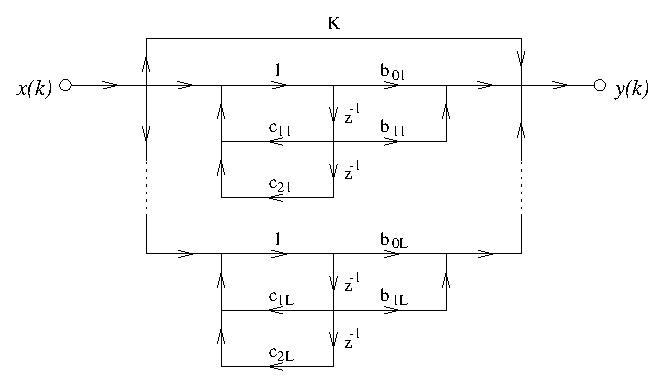
\includegraphics{iir-par}
  \end{center}
  \caption{\SF Parallel-form IIR filter block diagram.\label{IIR-filter}}
\end{figure}
%------------------ End of IIR filter -----------------------------------

In this context it is also necessary to simulate the convertion back
to and forth the analog domain, e.g. to simulate multiple transcodings
which are called {\em asynchronous trancodings}\footnote{\SF As the
name indicates, there is no synchronization between sampling instants
of the two digital systems, i.e., re-sampling in the succeeding A/D is
not synchronous to the clock in the preceding D/A converter.}. One
way to simulate asynchronous transcodings is by means of a non-linear
phase filter (non-constant group delay), which is most efficiently
implemented using IIR filters.

Infinite impulse response (IIR) filters used in this tool are of the
parallel form (see figure \ref{IIR-filter}), described by the
equation:
\[
    H_I^p(z) = K + \sum_{l=1}^{L}
                    { b_{0l}+b_{1l} z^{-1} \over
                      \ 1+c_{1l} z^{-1}+ c_{2l} z^{-2} \
                    }
\]
and of the cascade form (see figure \ref{IIR-cascade-filter}), described
by the equation:
\[
    H_I^c(z) = \prod_{l=1}^{N}
                    { b_{0l} + b_{1l} z^{-1} + b_{2l} z^{-2}\over
                           1 + c_{1l} z^{-1} + c_{2l} z^{-2}
                    }
\]

%------------------ Begin of cascade-form IIR filter --------------------
\begin{figure}
  \begin{center}
    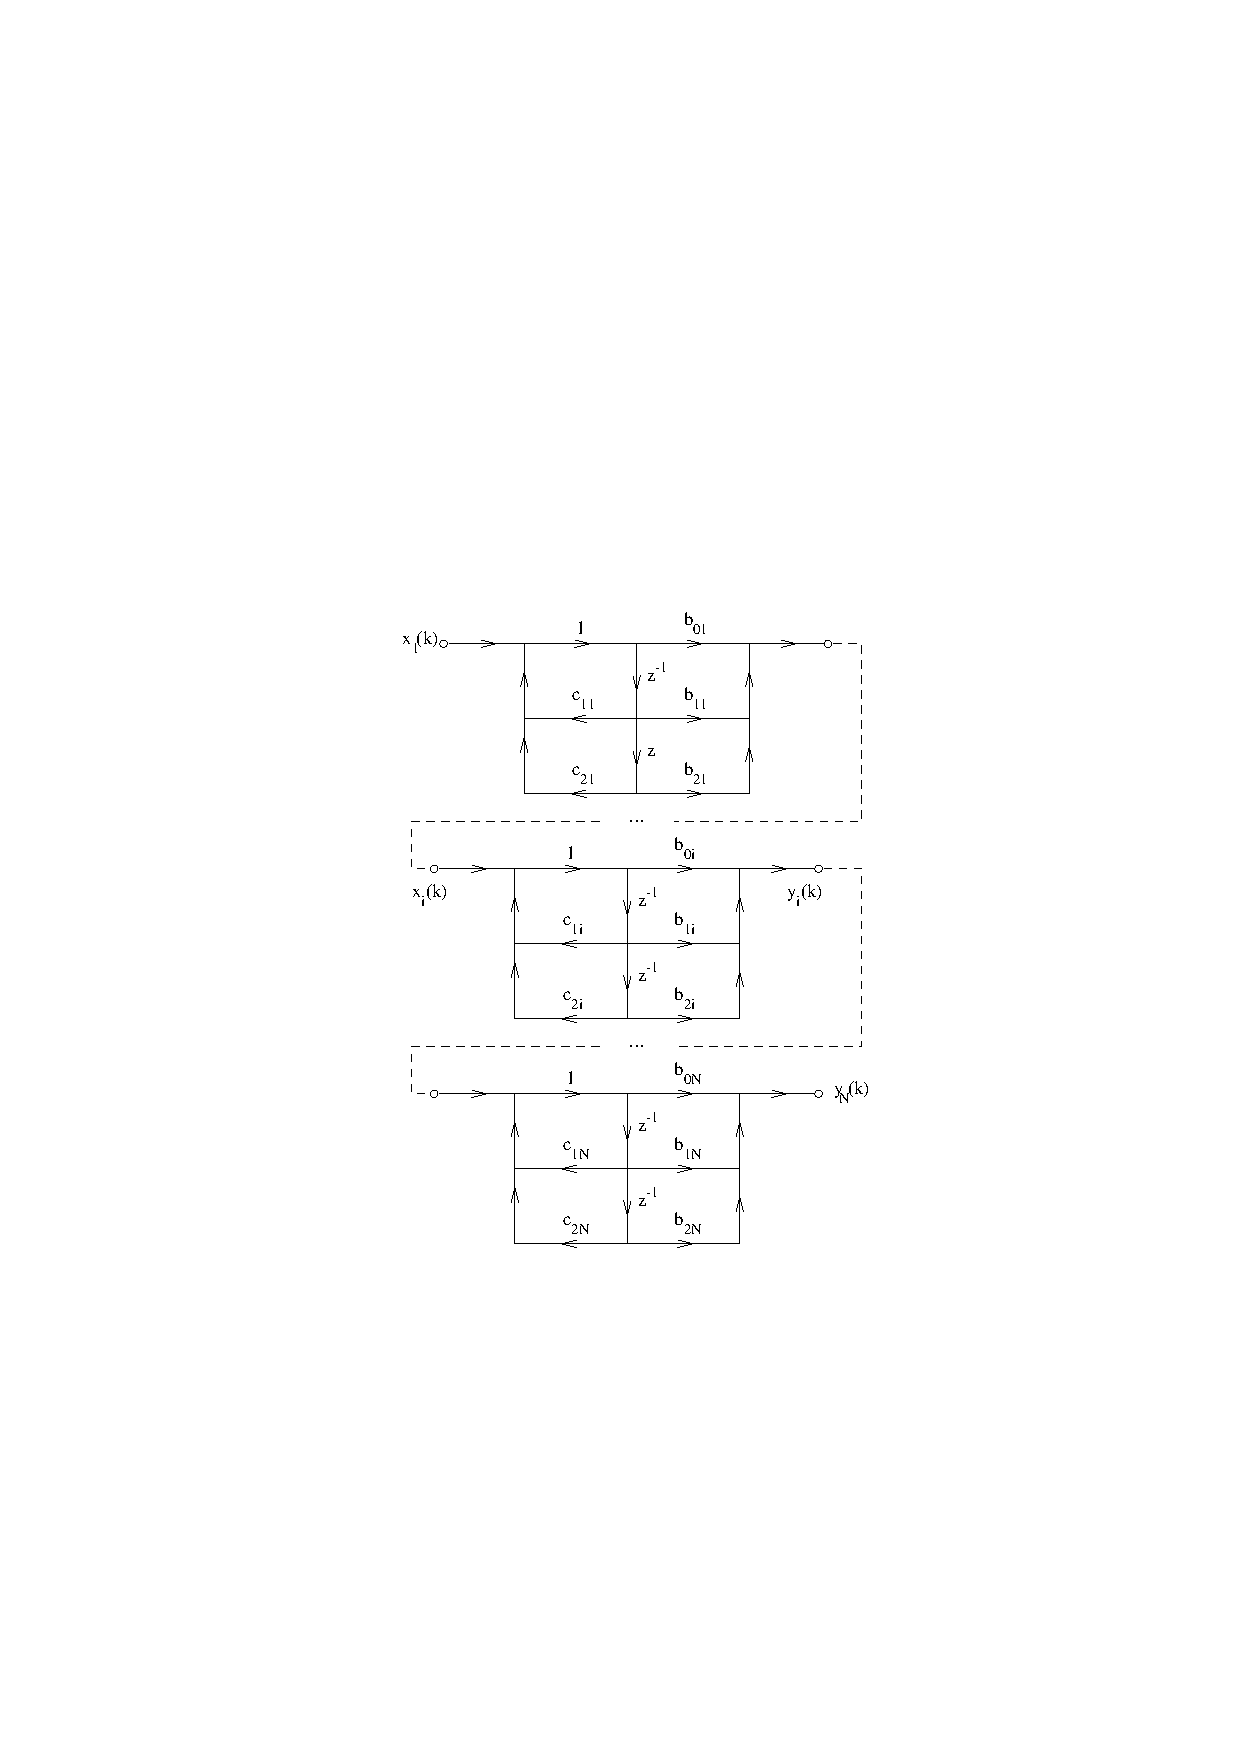
\includegraphics{iir-casc}
  \end{center}
  \caption{\SF Cascade-form IIR filter block diagram.
               \label{IIR-cascade-filter}}
\end{figure}
%------------------ End of IIR filter -----------------------------------


%=============================
\section{Implementation}

The rate change algorithm is organized in two modules, FIR and IIR,
with prototypes respectively in {\tt firflt.h} and {\tt iirflt.h}. It
evolved from a version initially developed as part of the ETSI
Half-rate GSM codec Host Laboratory exercise \cite{SCD-ETSI}. The
rate-change functionality was incorporated in the STL92 in two main
files, {\tt hqflt.c} and {\tt pcmflt.c}.  To make these routines more
flexible, the following modifications were included:
\begin{itemize}
 \item[FIR:] the FIR module was divided into a library source file ({\tt
        fir-lib.c}) containing the basic filtering and
        initialization functions, as well as into source files for each kind of
        filter: {\tt fir-flat.c} for high-quality low-pass and bandpass
        filters, {\tt fir-irs.c} for the classical and modified IRS
        filters, and so on;
 \item[IIR:] the IIR module was divided into a library file ({\tt
        iir-lib.c}) containing basic filtering and
        initialization functions, as well as into source files for each kind of
        filter: {\tt iir-g712.c} for G.712 filtering using the
        parallel-form filters, {\tt iir-flat.c} for flat bandpass 1:3
        and 3:1 asynchronization filtering using a cascade-form
        filter, and so on.
\end{itemize}

Files {\tt fir-*.c} of the FIR module contain all the routines
implementing FIR filters, i.e., the high-quality filters and IRS,
$\Delta_{SM}$ and psophometric weighing filters. Files {\tt iir-*.c}
of the IIR module implement the IIR filters, i.e., the parallel-form PCM
filter and the cascade-form 3:1 asynchronization filter.

Some of these filters have been implemented using 24-bit coefficients,
thus allowing real-time, bit-exact hardware implementation of these
routines. It may be noted that, for these filters in the STL, the
calculations are performed in floating-point arithmetics by converting
the coefficients from the range $\SF -2^{23}$..$\SF 2^{23}$--1 to $-1
.. +1$, which is not needed in real time hardware with fixed-point
DSPs.

Frequency response and impulse response plots are provided for the
STL filters in the forthcoming sections. It should be noted,
however, that the impulse responses shown have been computed from
the 16-bit quantized impulse responses of the filters, as generated
by the demonstration programs, while the frequency responses were
calculated as described in section \ref{RATE-Tests}. It should be
noted that the apparent asymmetry in some impulse responses happens
because an integer number of samples are generated, and linear
interpolation is used to draw the figure. If the impulse responses
were derived directly from the filter coefficients, the plot would
be symmetric.


\NOTE{158mm}{
                When the same filter type is used by several
                independent speech materials (e.g. several speech
                files) within the same execution of an application
                program, the user must remember that the filters have
                memory. Hence, wrong results can be obtained if a
                given number of initial samples are not discarded.
                See section \ref{Rate-exp} for an example, where the
                first 512 samples are skipped when calculating the
                power level of the output tone.
}


%-.-.-.-.-.-.-.-.-.-.-.-.-.-.-.-.-
\subsection{FIR module}

The frequency responses of the implemented high-quality low-pass
filters are shown in figures \ref{hq-frq-1-2} and \ref{hq-frq-1-3}
(for rate-change factors 2 and 3, respectively), while the telephone
bandwidth bandpass filter is given in figure \ref{hq-bandpass} (only
a rate-change factor of 2 is available). The impulse responses of
these filters are given in figures \ref{ir-hq-up}, \ref{ir-hq-down},
and \ref{ir-bandpass}, respectively for the up-sampling filters
(factors 2 and 3), for the down-sampling filters (factors 2 and 3),
and for the bandpass filter.

The transmit-side IRS filter has been implemented for the ``regular''
and modified flavors. The regular transmit-side P.48 IRS filter
amplitude responses are shown in figure \ref{tx-reg-irs-frq} (the
available sampling rates are 8 and 16 kHz). The transmit-side modified
IRS filter is available for sampling at 16 kHz and 48 kHz, and
their frequency responses are shown in figure \ref{tx-mod-irs-frq}.
The impulse response of these transmit-side IRS filters are in figures
\ref{tx-reg-irs-ir} and \ref{tx-mod-irs-ir} for the regular and
modified IRS filters, respectively. The receive-side modified IRS
filter has also been implemented and the frequency responses for 8 kHz
and 16 kHz sampling rate are found in figure \ref{rx-mod-irs-frq}. The
impulse responses of the receive-side modified IRS filters are shown in
figure \ref{rx-mod-irs-ir}.

The frequency response of the STL psophometric filter is given in
figure \ref{pso-08k-frq}, and that of the $\Delta_{SM}$ filter in figure
\ref{delta-sm-frq}.

For wideband signals, three weighting filters are available. The
transmit-side ITU-T P.341 filter amplitude response is shown in
figure \ref{tx-p341-frq}, and its impulse response is shown in
figure \ref{tx-p341-ir}. Alternatively to the P.341 filter, the
frequency and impulse responses of the two bandpass filters,
50 Hz-5 kHz bandpass filter and 100 Hz -5 kHz, are shown, respectively,
in figures \ref{bp5k-16k-frq} and \ref{bp5k-16k-ir}, and in figures
\ref{bp100_5k-16k-frq} and \ref{bp100_5k-16k-ir}.

For super wideband signals, four weighting filters are available.
The 50 Hz-14 kHz bandpass filter, extension of ITU-T P.341 filter, is
presented in figures \ref{50_14k-32k-frq} (frequency response), and
\ref{50_14k-32k-ir} (impulse response). Alternatively to this P.341
filter extension, the frequency responses of the three MUSHRA
anchors filters, LP3.5, LP7 and LP10 filters, are shown in figures
\ref{LP35-frq}, \ref{LP7-frq} and \ref{LP10-frq}, respectively.
Their impulse responses are shown in figures \ref{LP35-ir},
\ref{LP7-ir} and \ref{LP10-ir}, respectively.

The high-quality filters were implemented for rate-change factors
of 2 and 3. The IRS filters, band-limiting filters and MUSHRA
anchors have been designed for specific {\em sampling rates} (e.g.
8 and 48 kHz). It should be noted that, while the high-quality
filters are independent of the rate, these filters are not,
because their masks are specified in terms of Hz, rather than
normalized frequencies. This means that to carry out a
high-quality up-sampling from 8 to 16 kHz, and from 16 to 32 kHz,
the same routines are called, while for IRS, band-limiting or
MUSHRA anchors, there is no rate-change routine from 16 to 32 kHz.

Since the digital filters have memory, state variables are needed. In
this version of the STL, a type {\tt SCD\_FIR} is defined, containing the past
sample memory, as well as filter coefficients and other control
variables. Its fields, whose values shall never be changed by the
user, are as follows:
\begin{quote} \normalsize
 {\em lenh0}    \dotfill \parbox{110mm}{\SF Number of FIR coefficients}\\
 {\em dwn\_up}  \dotfill \ \parbox{110mm}{\SF Down-sampling factor }\\
 {\em k0}       \dotfill \parbox[t]{110mm}{\SF Start index in next segment
                                       (needed in segment-wise filtering) }\\
 {\em h0}       \dotfill \parbox{110mm}{\SF Pointer to array with FIR
                                          coefficients }\\
 {\em T}        \dotfill \parbox{110mm}{\SF Pointer to delay line }\\
 {\em hswitch}  \dotfill \parbox{110mm}{\SF Switch to FIR-kernel: up- or down-
                                          sampling }\\
\end{quote}

The relevant routines for each module are described in the next
sections.\footnote{\SF It should be noted that in the source code
files there are local (privately-defined) functions which are not
intended to be directly accessed by the user and therefore are not
described here.}


%----------- Begin of FIR filters response : frq for factor 2 ---------------
\begin{figure}[hbtp]
  \begin{center}
    %Both boxes' dimension: 15.24cm x  8.89cm
        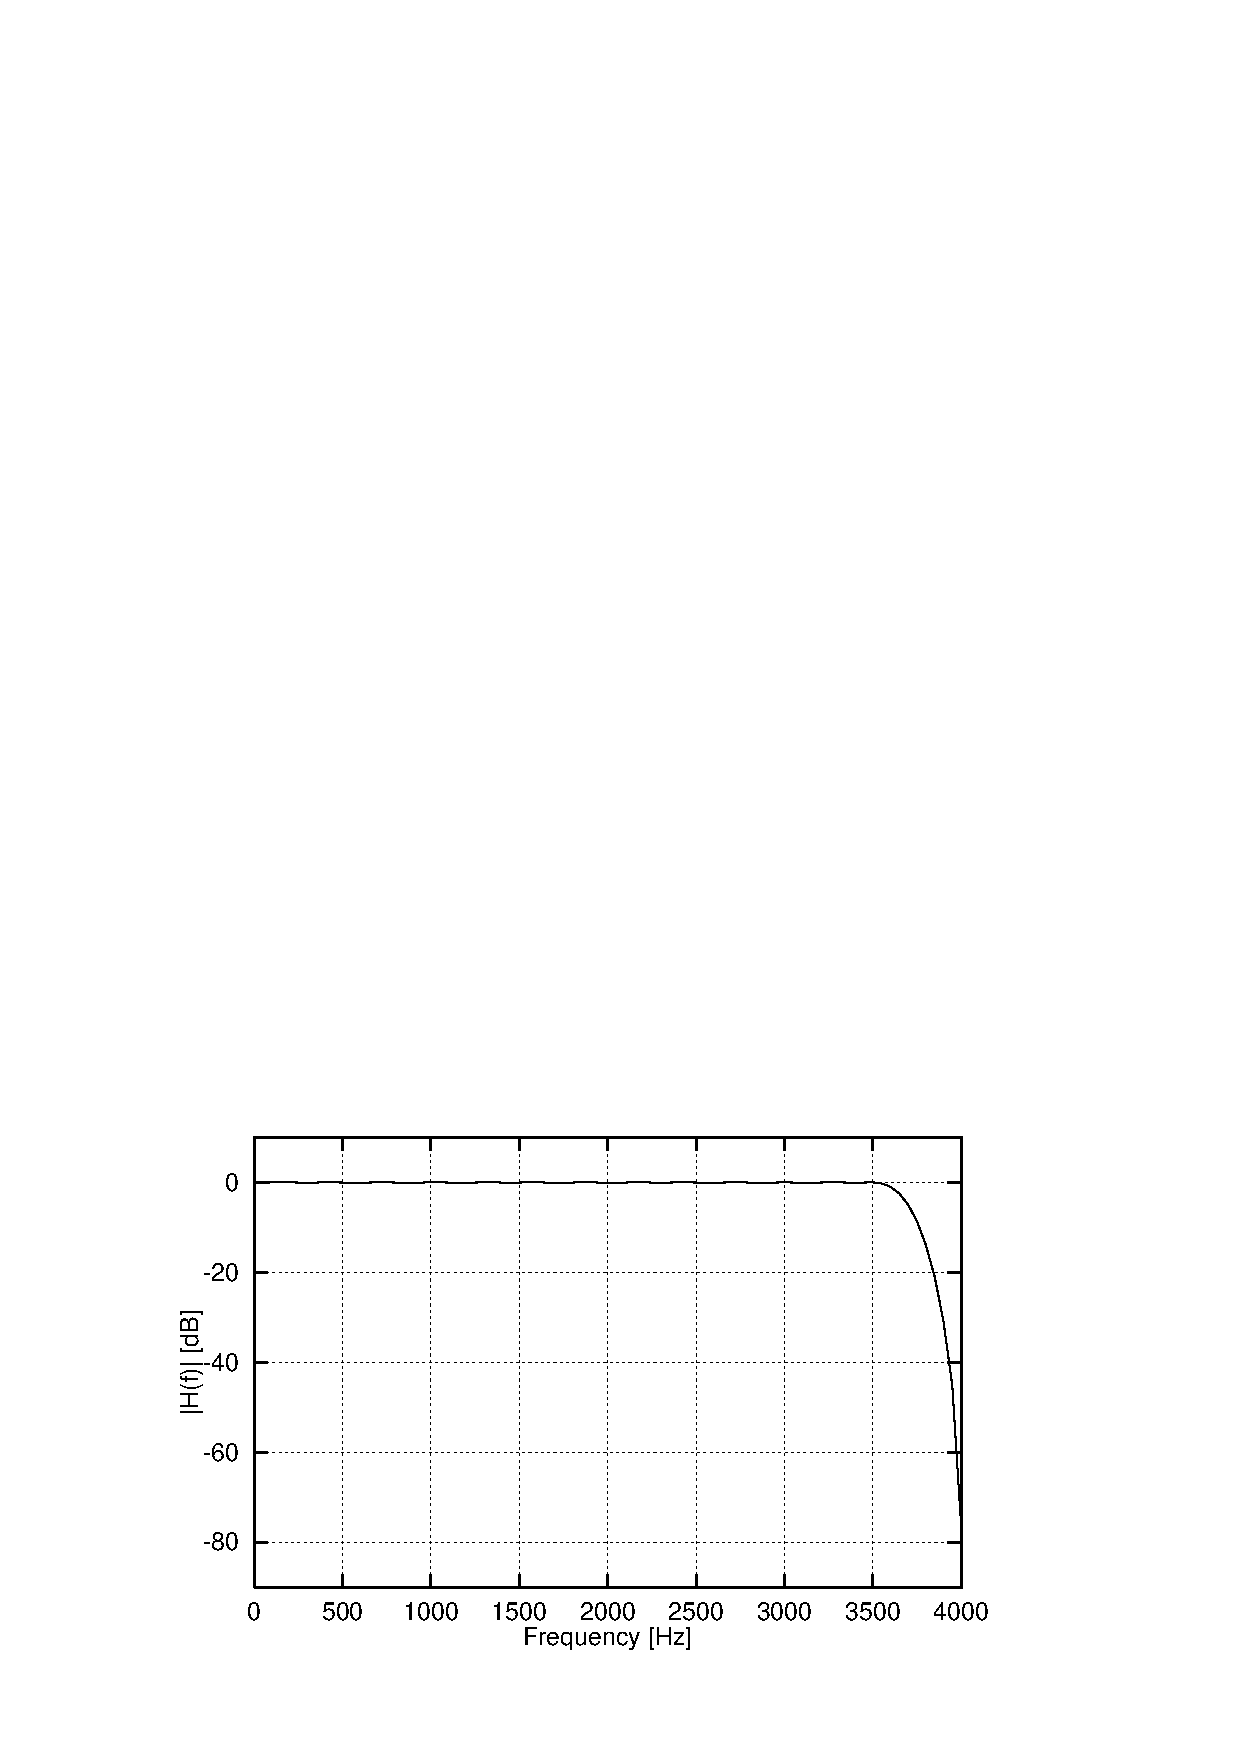
\includegraphics{hq2_1_2}
    \\
   (a) High-quality filter for up-sampling.

        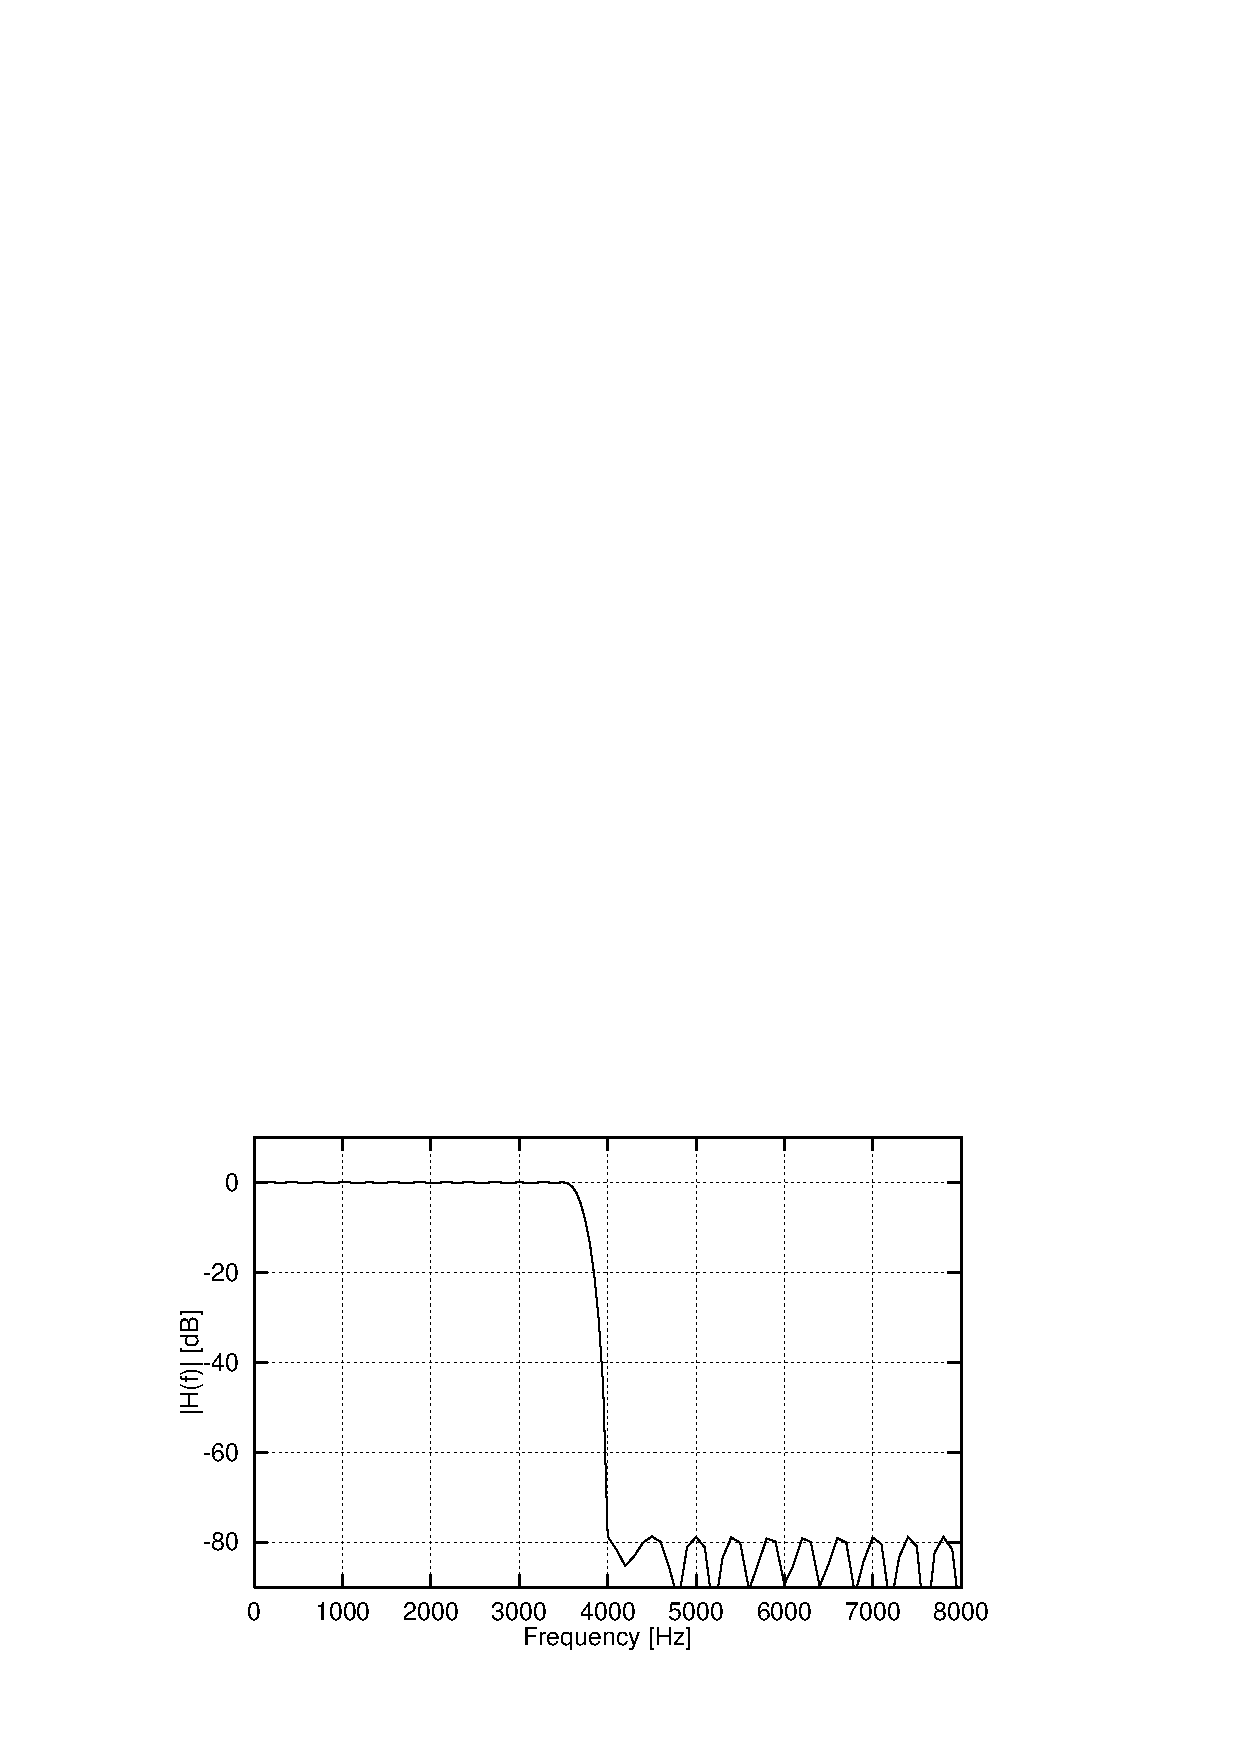
\includegraphics{hq2_2_1}
    \\
   (b) High-quality filter for down-sampling.

  \end{center}
  \caption{\SF High-quality filter responses for a
               factor of 2 and sampling rates of 8000 and
               16000 Hz.\label{hq-frq-1-2}}

\end{figure}
%------------- End of FIR filters response: frq for factor 2 ----------------

%----------- Begin of FIR filters response: frq for factor 3 ---------------
\begin{figure}[hbtp]
  \begin{center}
    %Both boxes' dimension: 15.24cm x  8.89cm
        \includegraphics{hq3_1_3}
    \\
   (a) High-quality filter for up-sampling.

        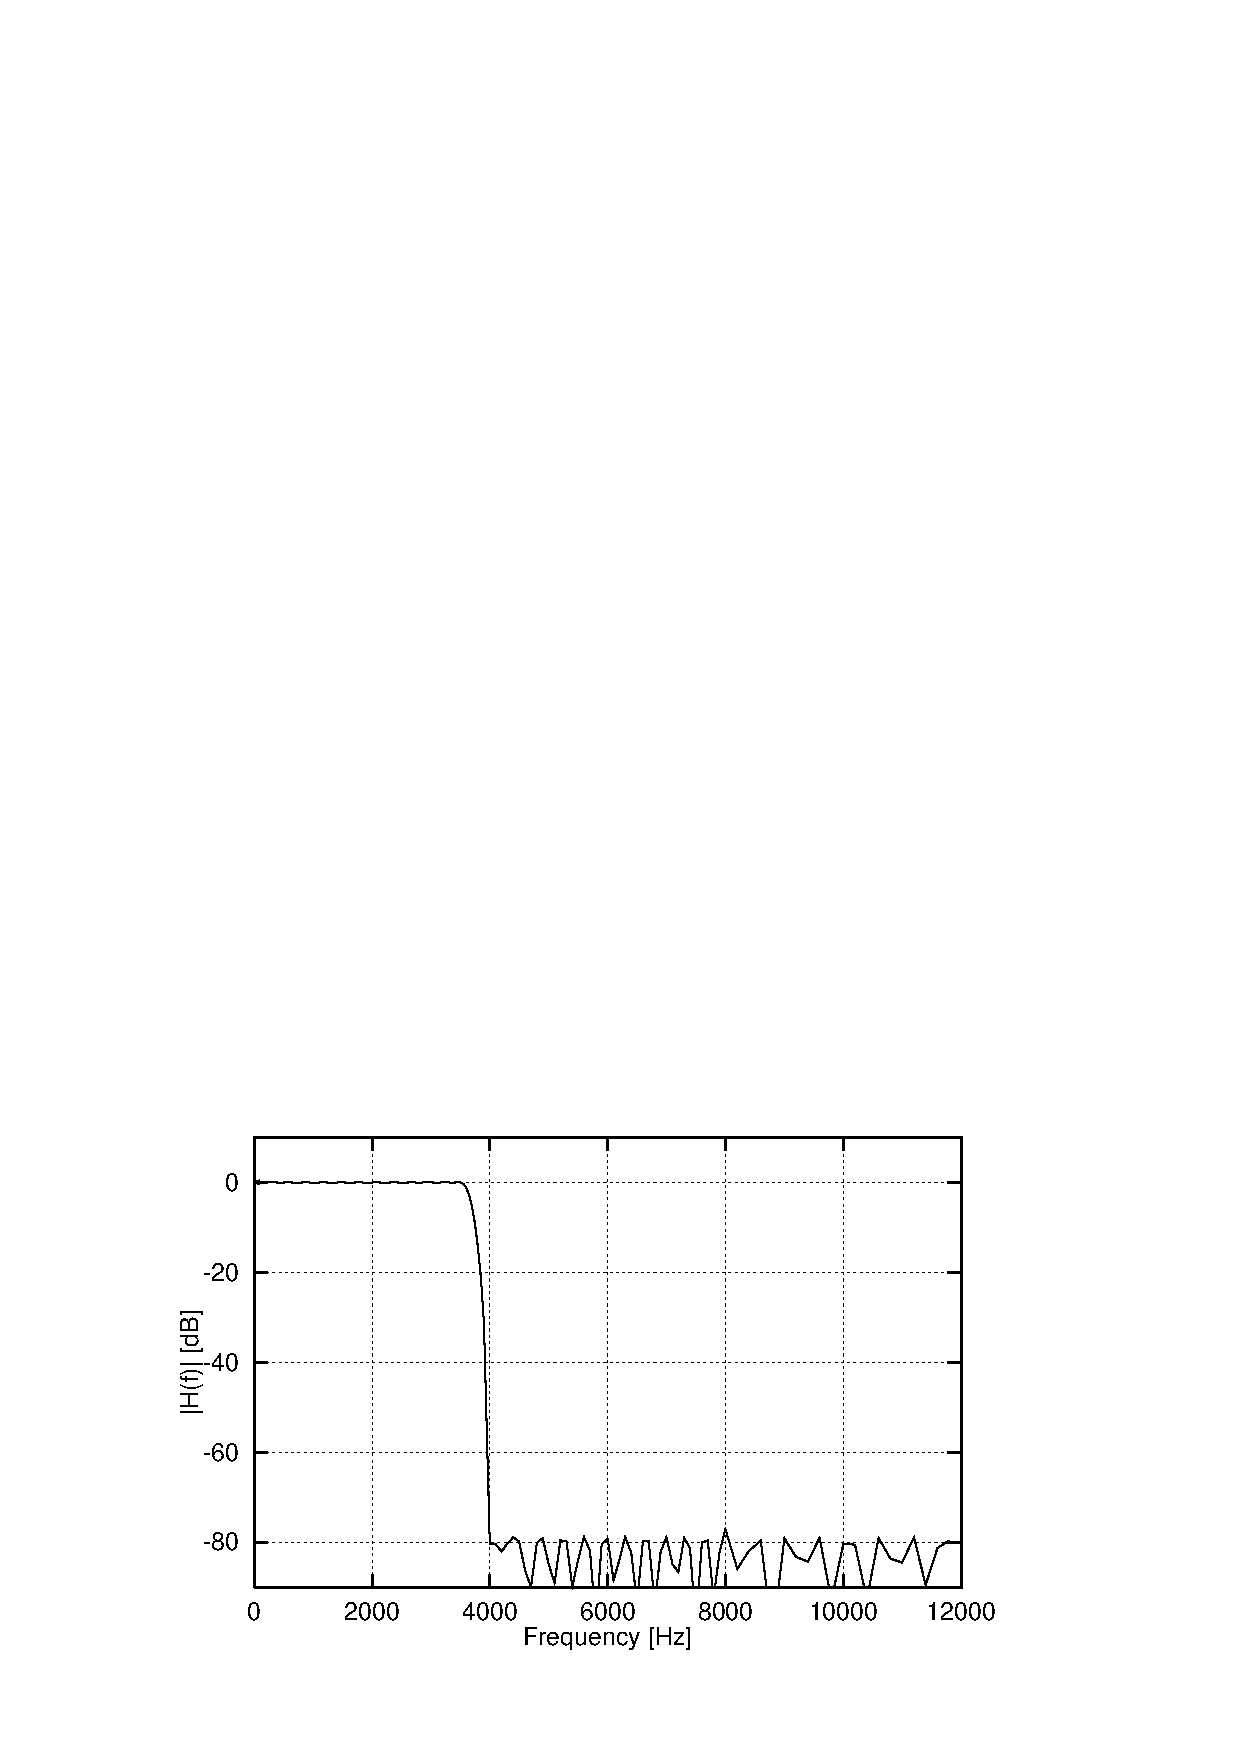
\includegraphics{hq3_3_1}
   \\
   (b) High-quality filter for down-sampling.

  \end{center}
  \caption{\SF High-quality filter responses for a
               factor of 3 and sampling rates of 8000 and
               24000 Hz.\label{hq-frq-1-3}}

\end{figure}
%------------- End of FIR filters response: frq for factor 3 ----------------


%----------- Begin of FIR filters response: frq for bandpass filter  --------
\begin{figure}[hbtp]
  \begin{center}
 \includegraphics{flat_1_2}
 \\
   (a) High-quality bandpass for up-sampling (factor 1:2).

 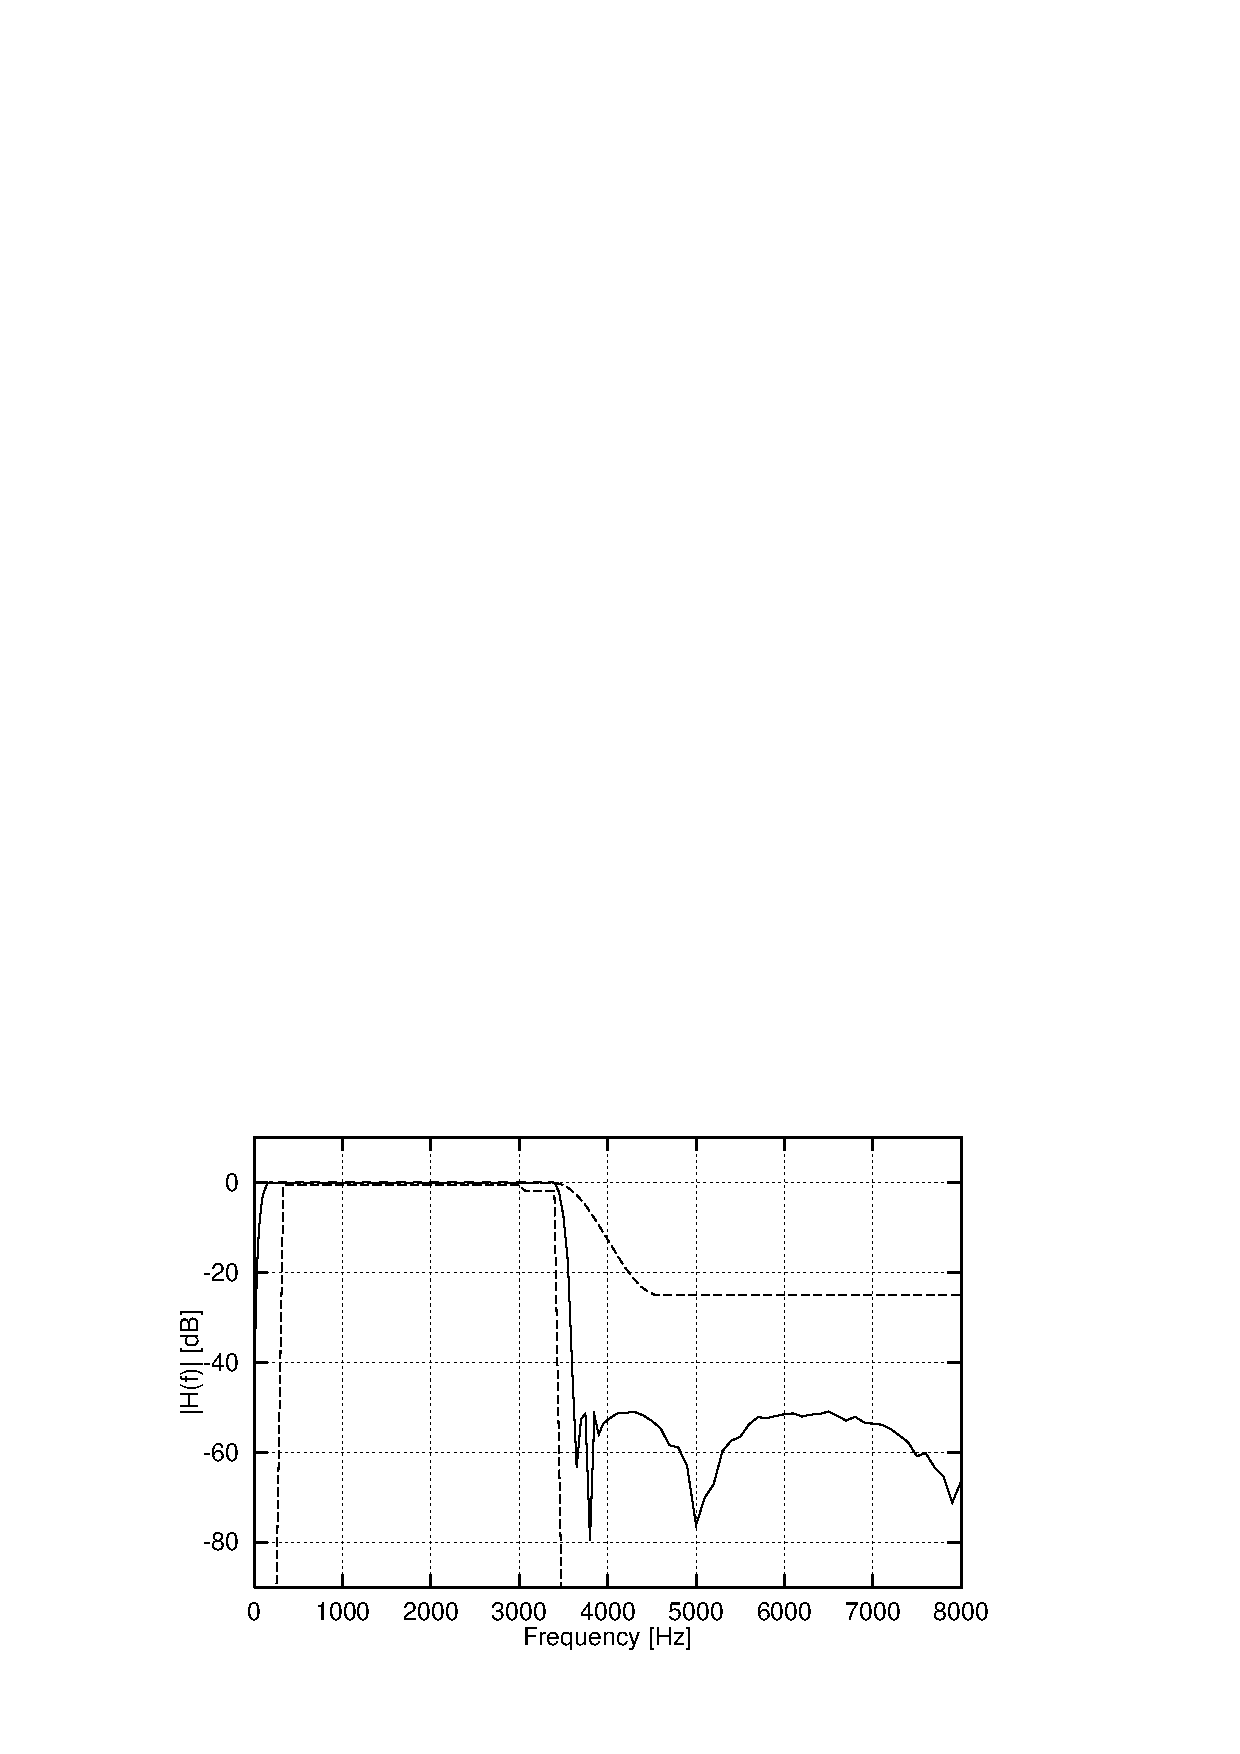
\includegraphics{flat_2_1}
 \\
   (b) High-quality bandpass for 2:1 down-sampling or for 1:1
       filtering.

  \end{center}
  \caption{\SF High-quality bandpass filter responses. Mask shown is
           that of the G.712 filter, for reference.
           \label{hq-bandpass}
          }
\end{figure}
%------------- End of FIR filters response: frq for bandpass ----------------


%--- Begin of FIR filters response: impulse response for UP filters ------
%Box dimension: 16.05cm x 18.03cm
\begin{figure}[hbtp]
  \begin{center}
 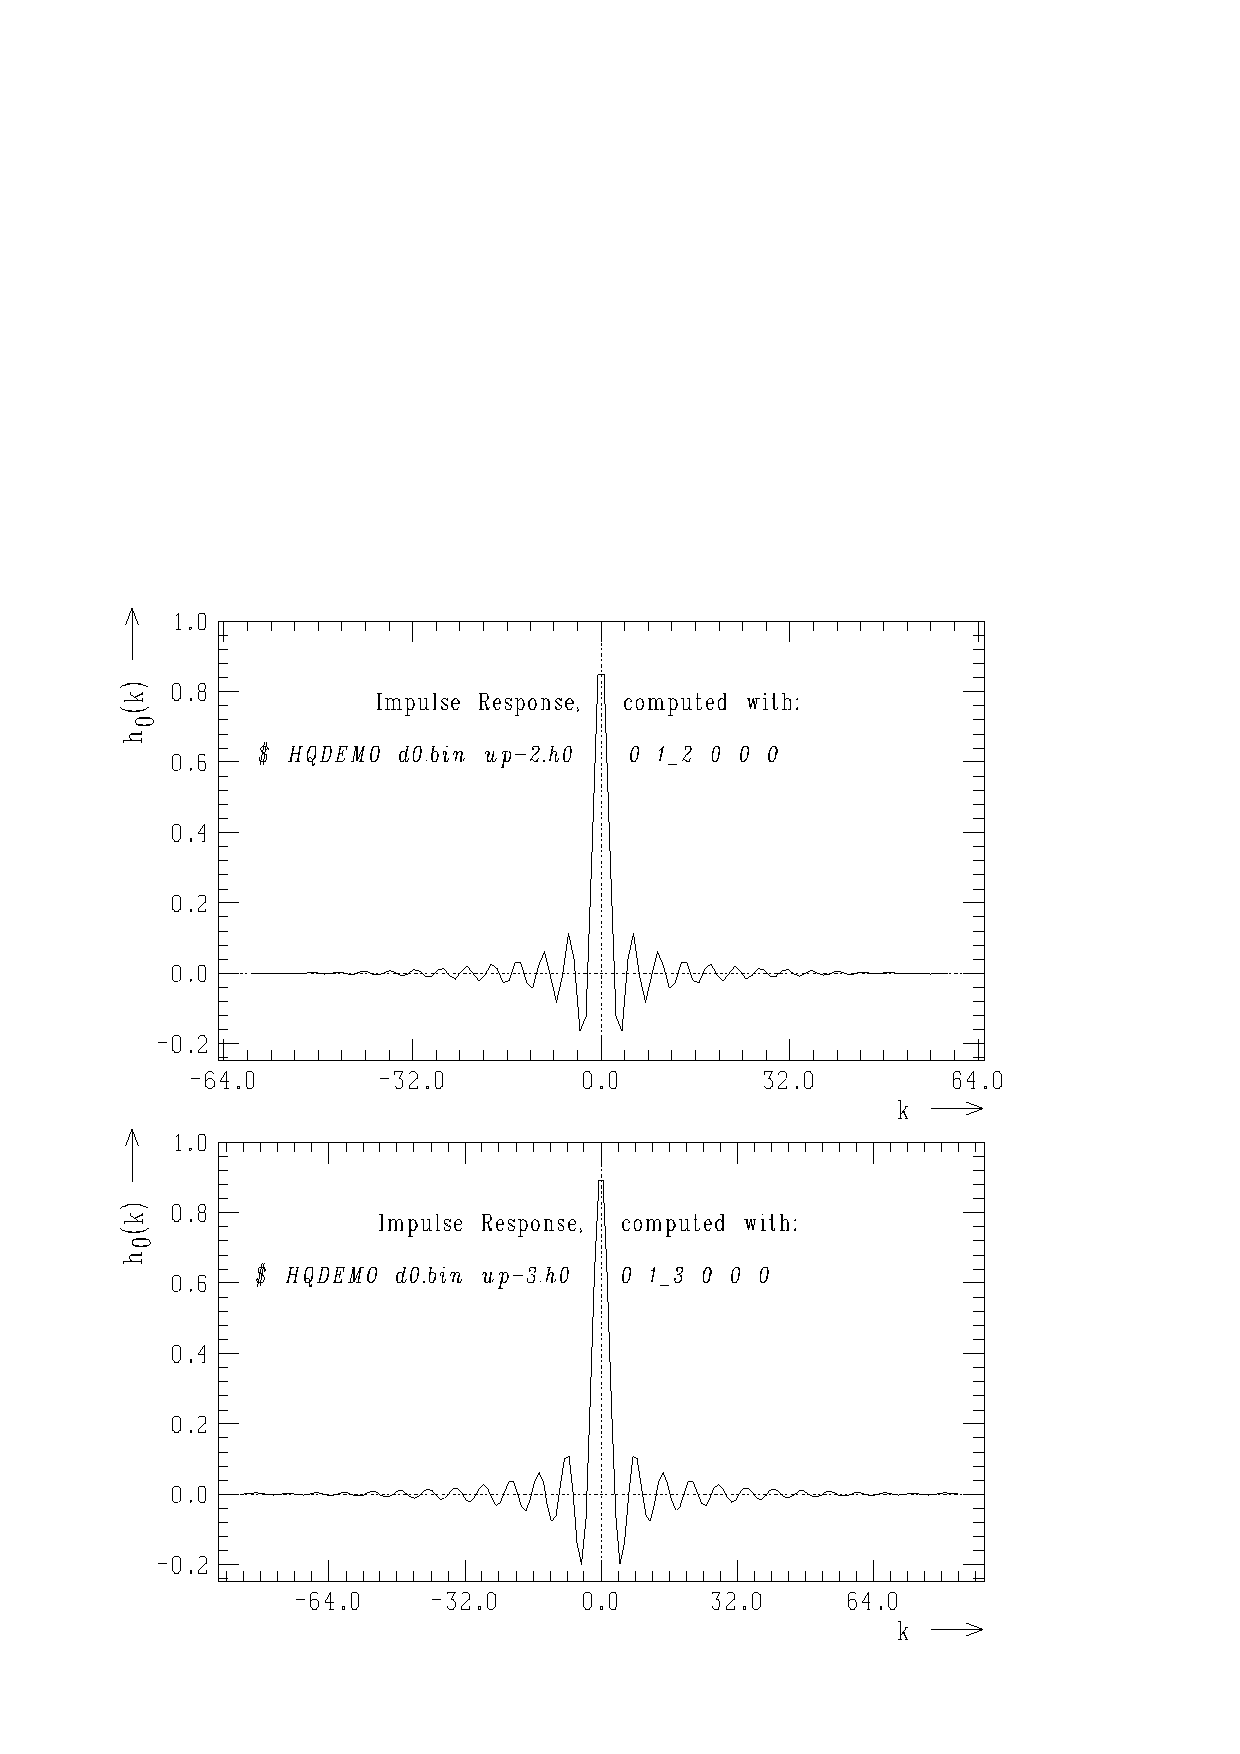
\includegraphics{hqup-h0}
  \end{center}
  \caption{\SF Impulse response for high-quality
               up-sampling filters (top, factor of 2; bottom,
               factor of 3).\label{ir-hq-up}}
\end{figure}
%----- End of FIR filters response: impulse response for UP filters ------


%--- Begin of FIR filters response: impulse response for DOWN filters ------
%Box dimension: 16.05cm x 18.03cm
\begin{figure}[hbtp]
  \begin{center}
 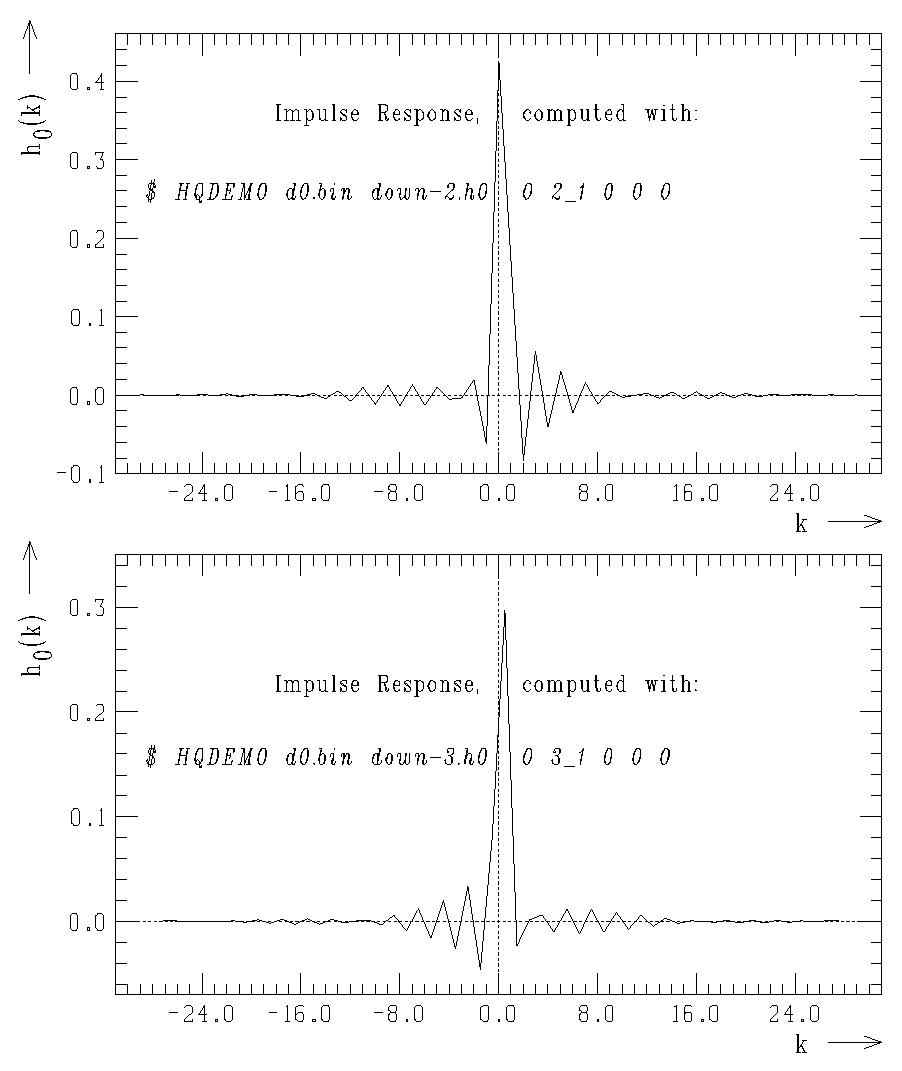
\includegraphics{hqdw-h0}
  \end{center}
  \caption{\SF Impulse response for high-quality
               down-sampling filters (top, factor of 2;
               bottom, factor of 3).\label{ir-hq-down}}
\end{figure}
%----- End of FIR filters response: impulse response for DOWN filters ------


%--- Begin of FIR filters response: impulse response for bandpass filter ----
%Box dimension: 16.05cm x 18.03cm
\begin{figure}[hbtp]
  \begin{center}
 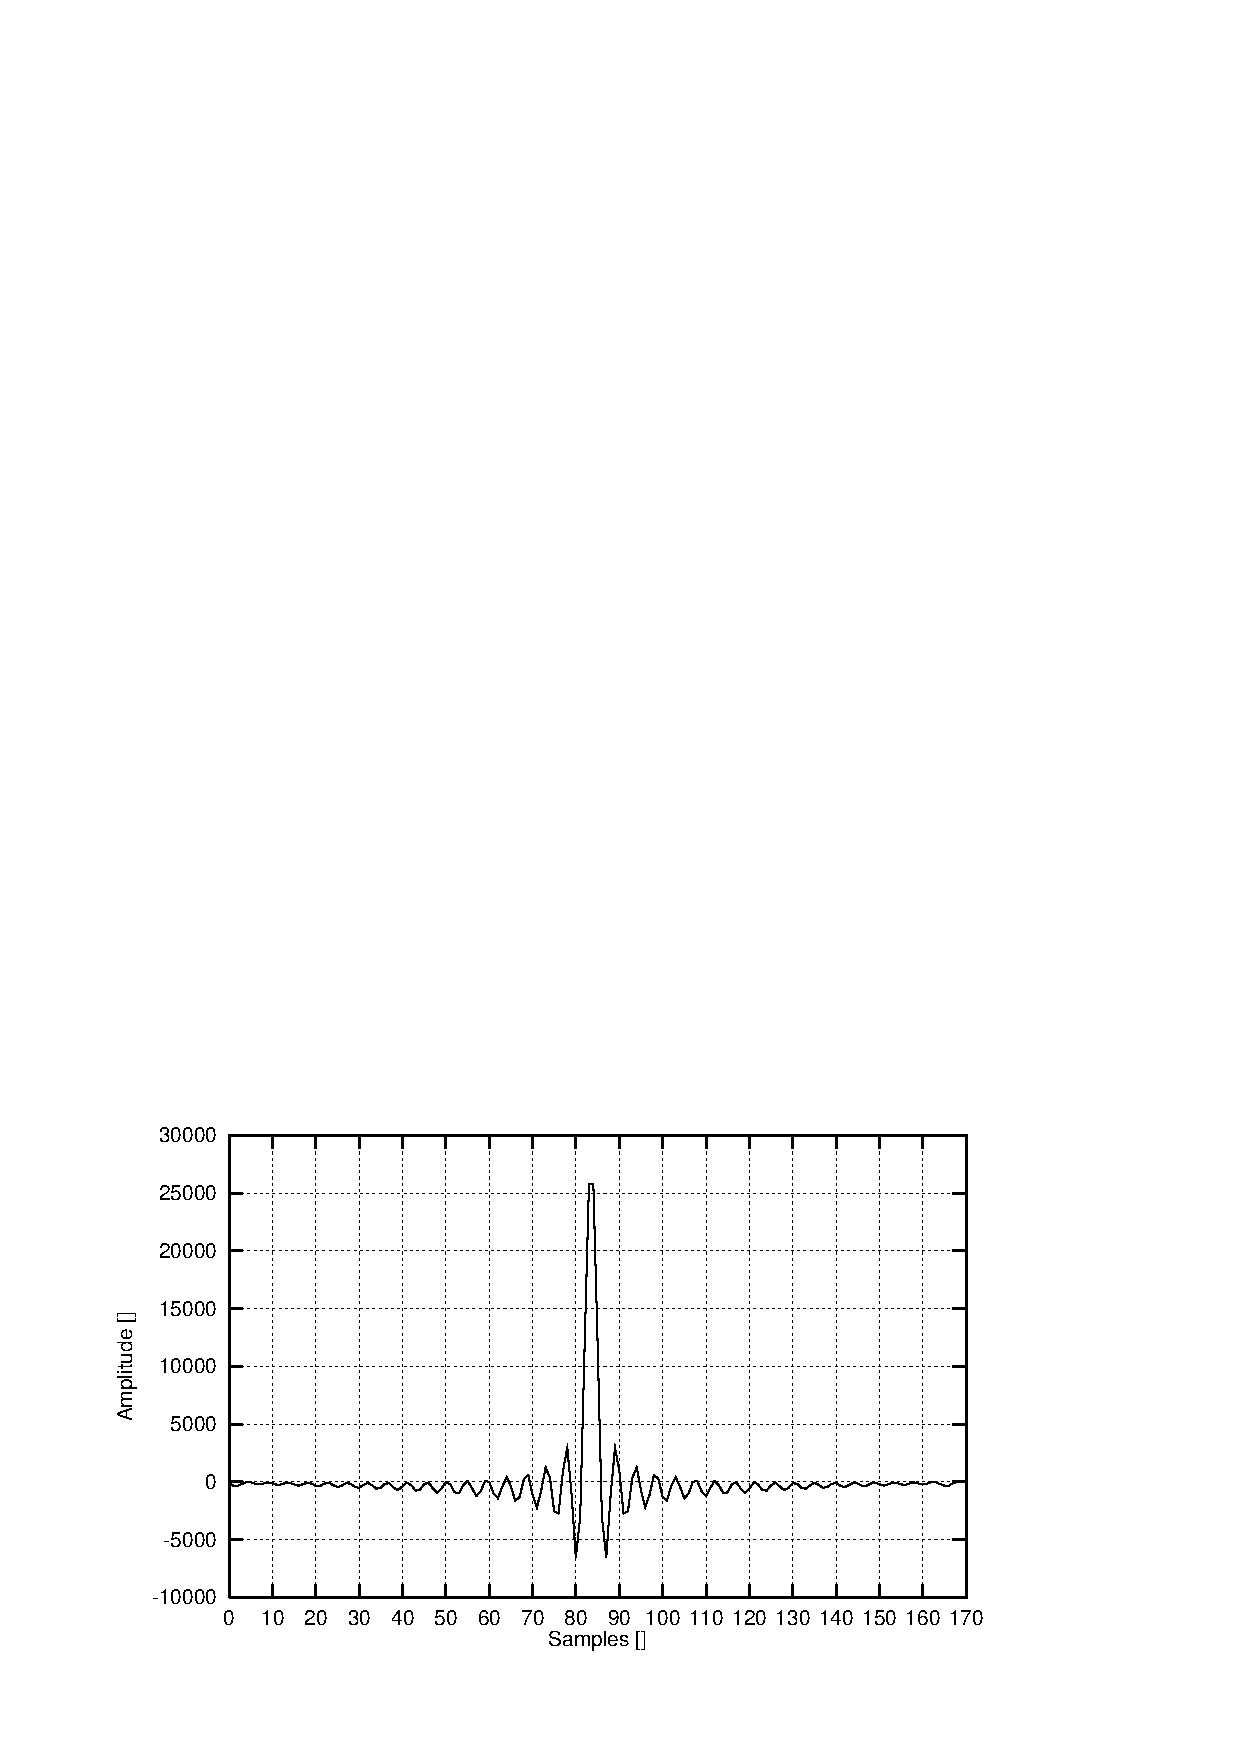
\includegraphics{bpup-h0}
 \\
   (a) High-quality bandpass for up-sampling (factor 1:2).

 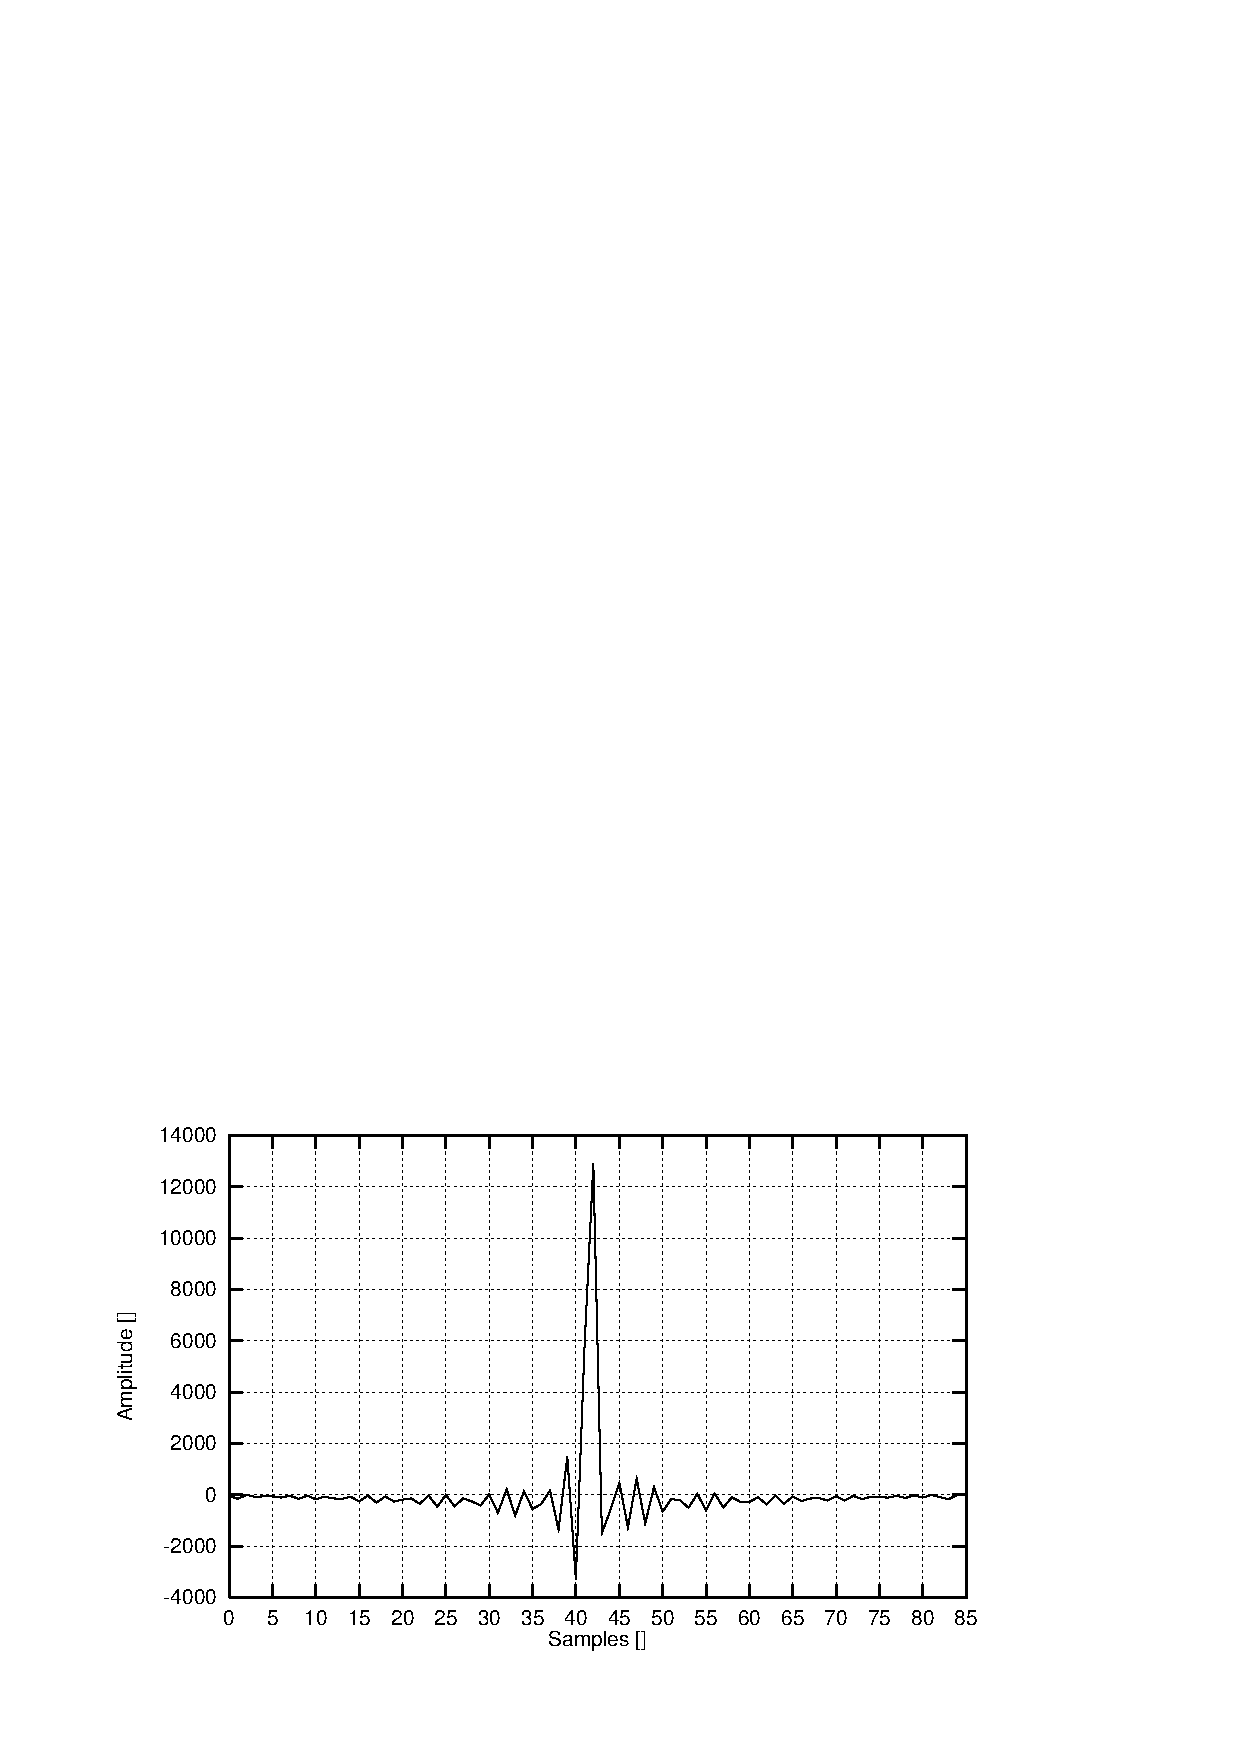
\includegraphics{bpdw-h0}
 \\
   (b) High-quality bandpass for down-sampling (factor 2:1).

  \end{center}
  \caption{\SF Impulse response for high-quality
               bandpass filter (factors 2:1 and 1:1). Top is
               up-sampling by a factor of 1:2, and bottom is
               down-sampling by a factor of 2:1. \label{ir-bandpass}}
\end{figure}
%----- End of FIR filters response: impulse response for bandpass filter ---


%----------- Begin of FIR filters response: frq for MSIN filter  --------
\begin{figure}[hbtp]
  \begin{center}
 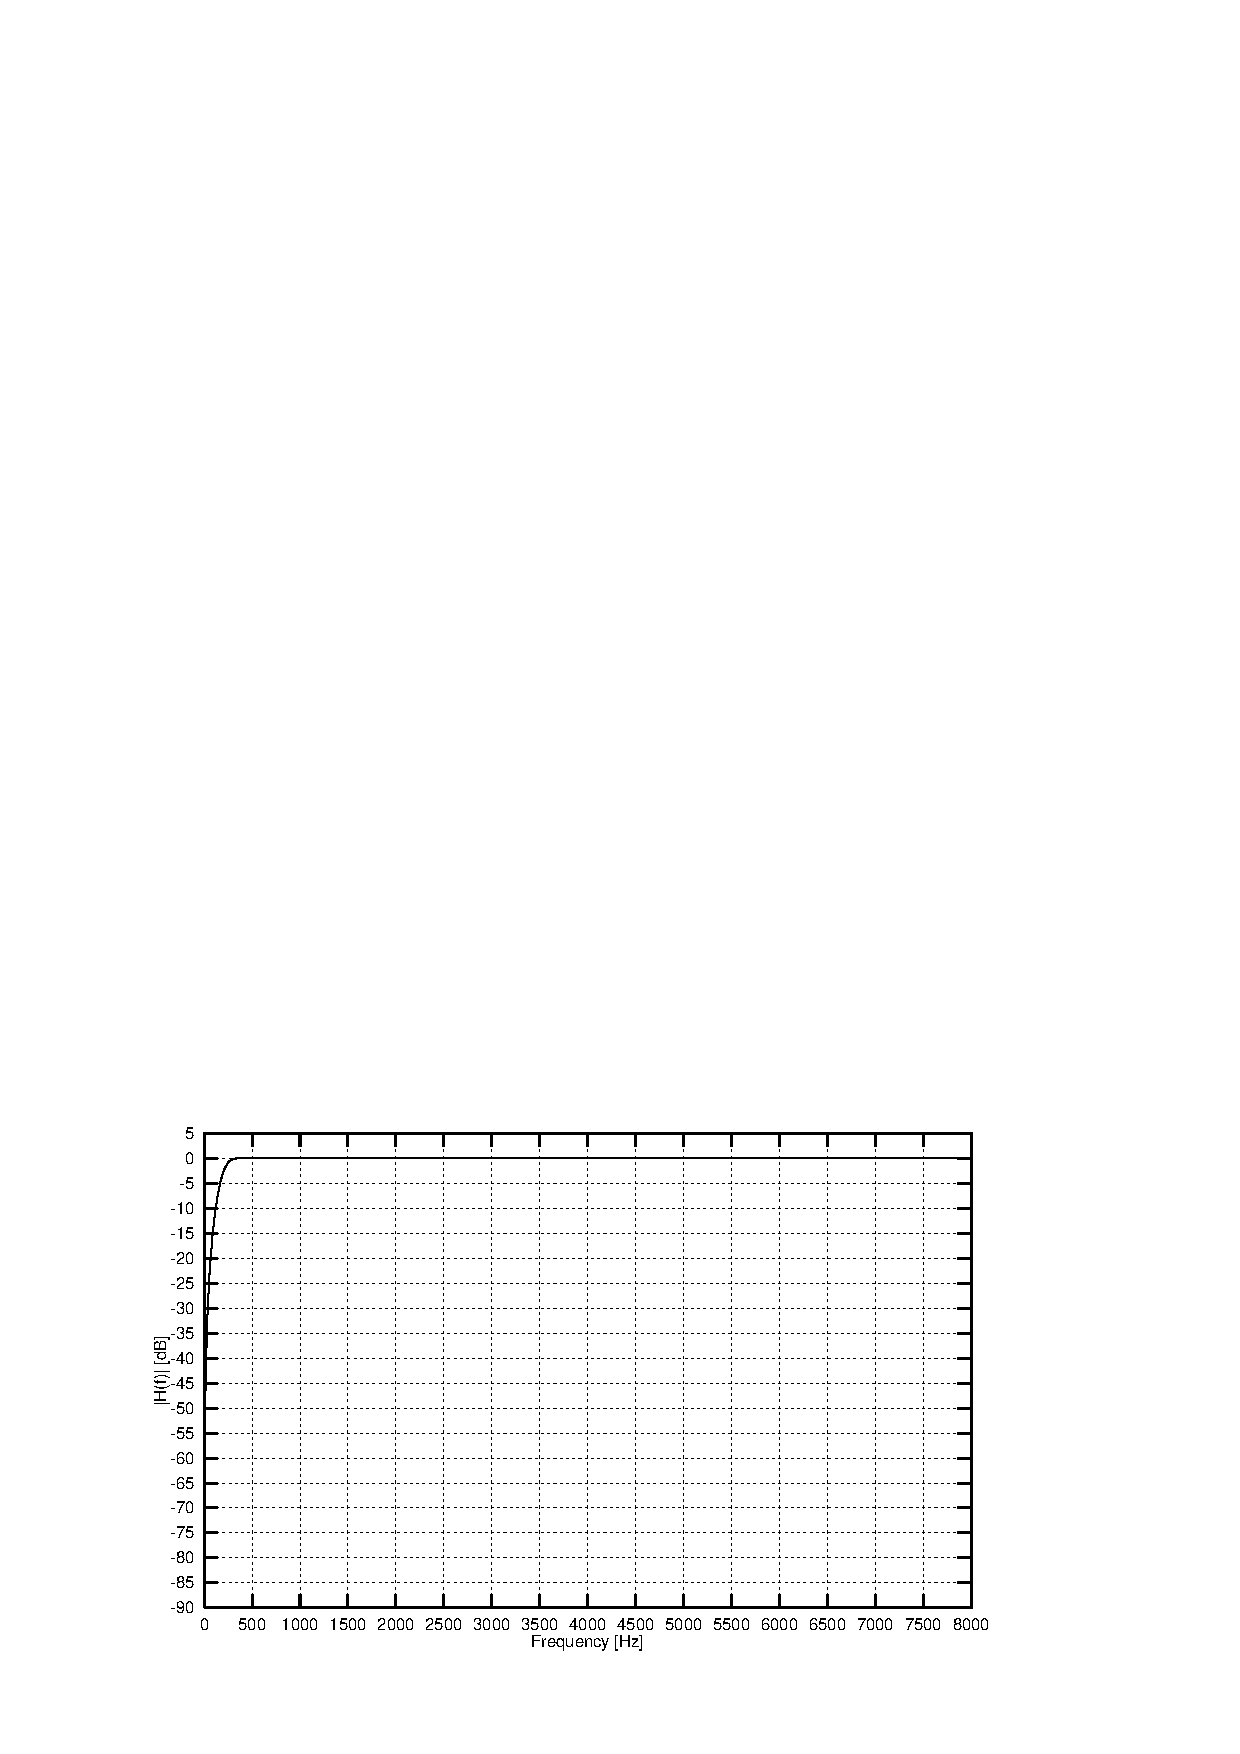
\includegraphics{msin16}
  \end{center}
  \caption{\SF STL mobile station input (MSIN) frequency response for data
               sampled at 16 kHz (factor 1:1).
           \label{msin-frq}
          }
\end{figure}
%------------- End of FIR filters response: frq for MSIN ----------------


%--- Begin of FIR filters response: impulse response for MSIN --------
\begin{figure}[hbtp]
  \begin{center}
 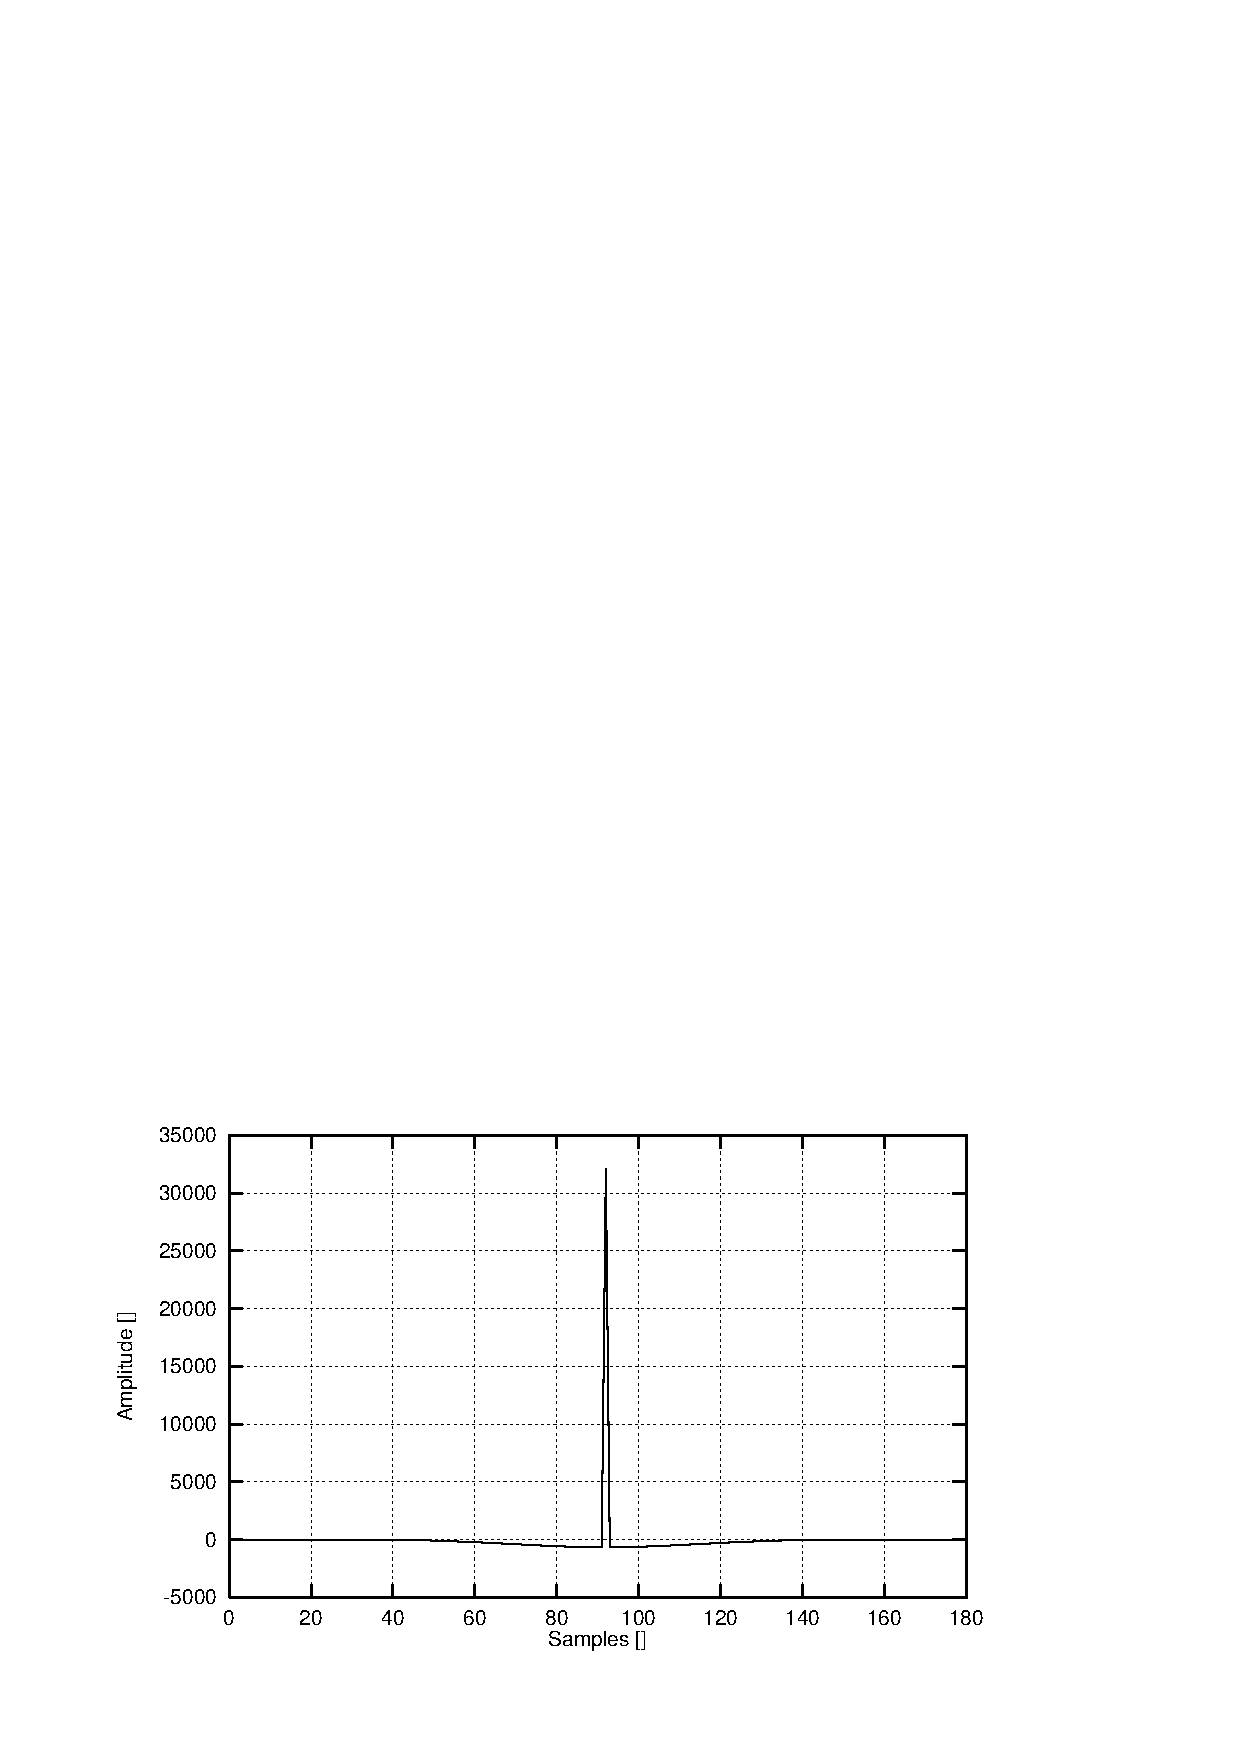
\includegraphics{msin16-h0}
  \end{center}
  \caption{\SF STL MSIN send-side filter impulse response.
           \label{msin-ir}
          }
\end{figure}
%----- End of FIR filters response: impulse response for MSIN -----

\flushfloats

%------------------ Begin of regular IRS filters response --------------------
\begin{figure}[hbtp]
  \begin{center}
 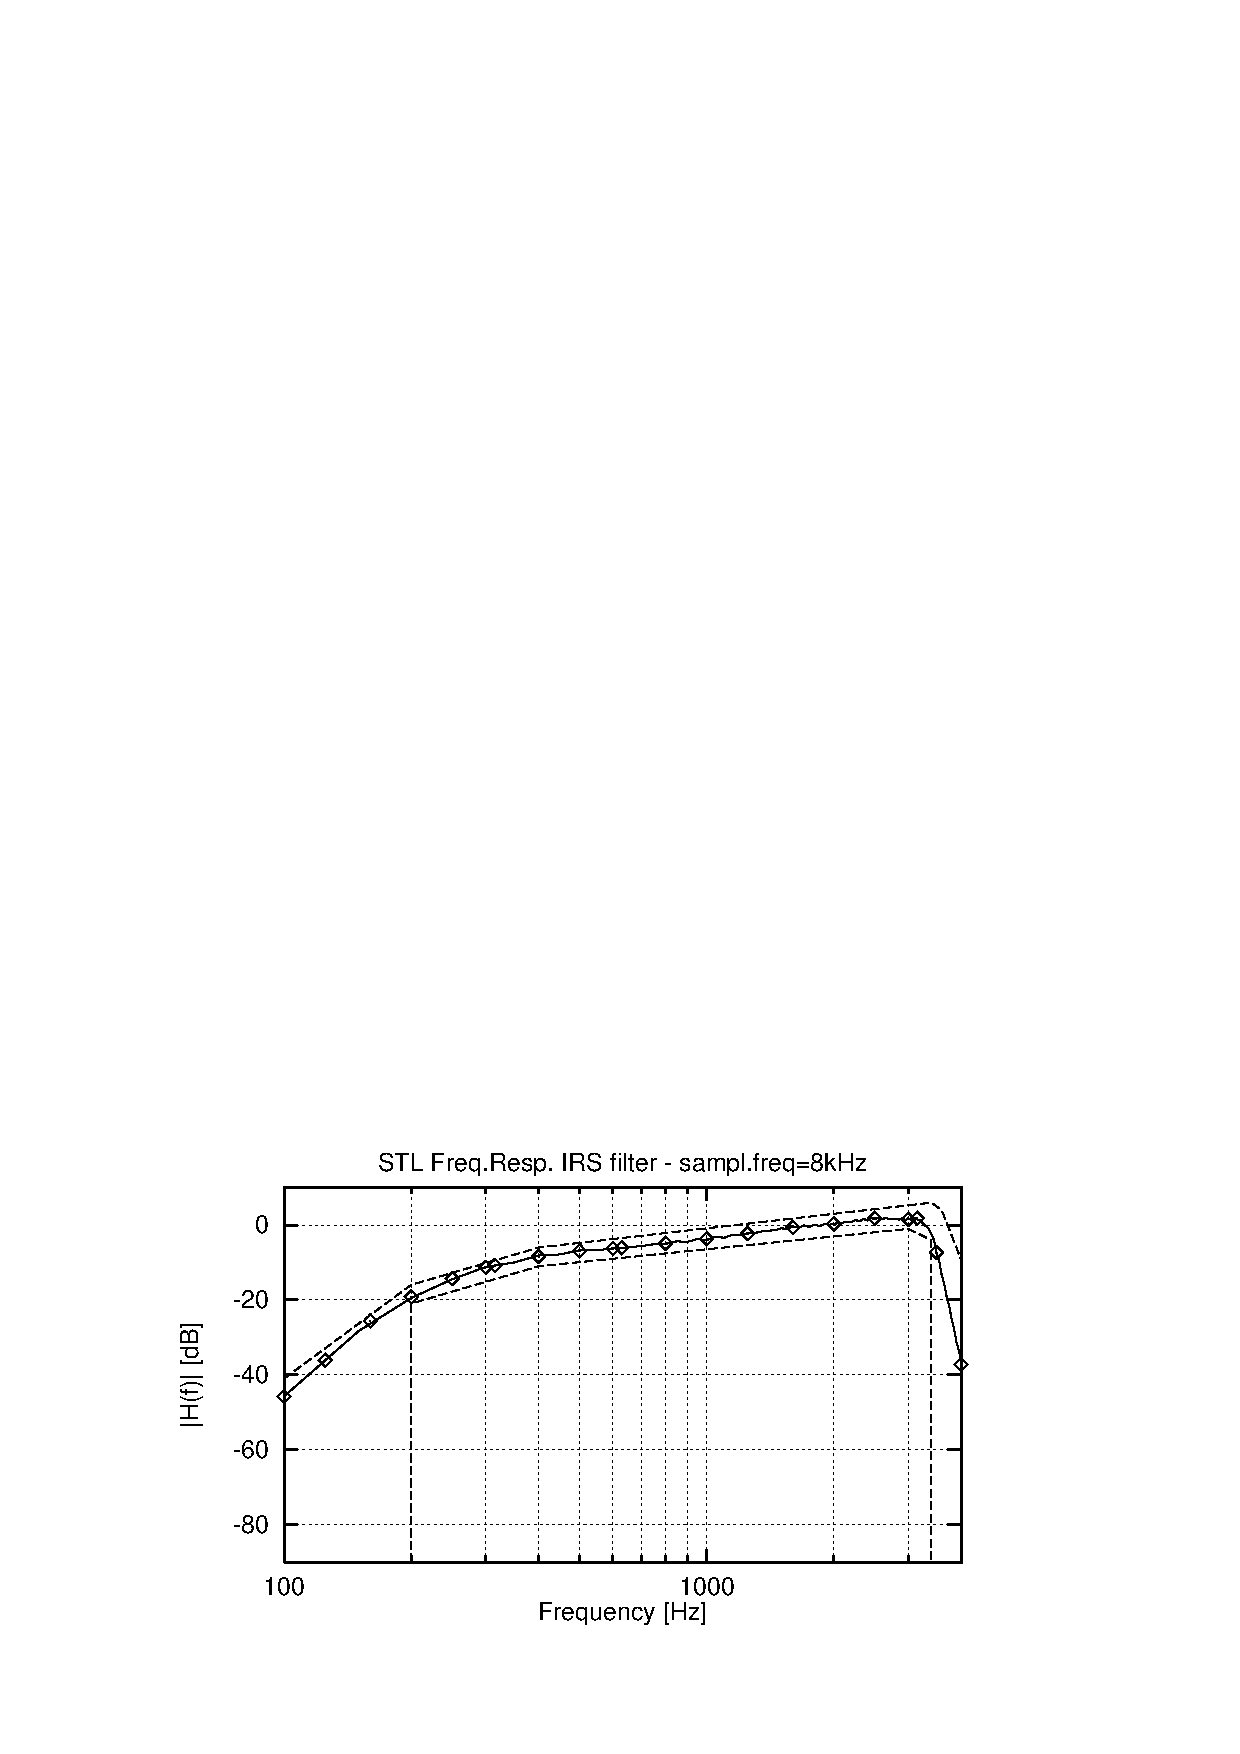
\includegraphics{irs_1_2}
 \\
   (a) Transmission-side IRS for input samples at 8 kHz.

 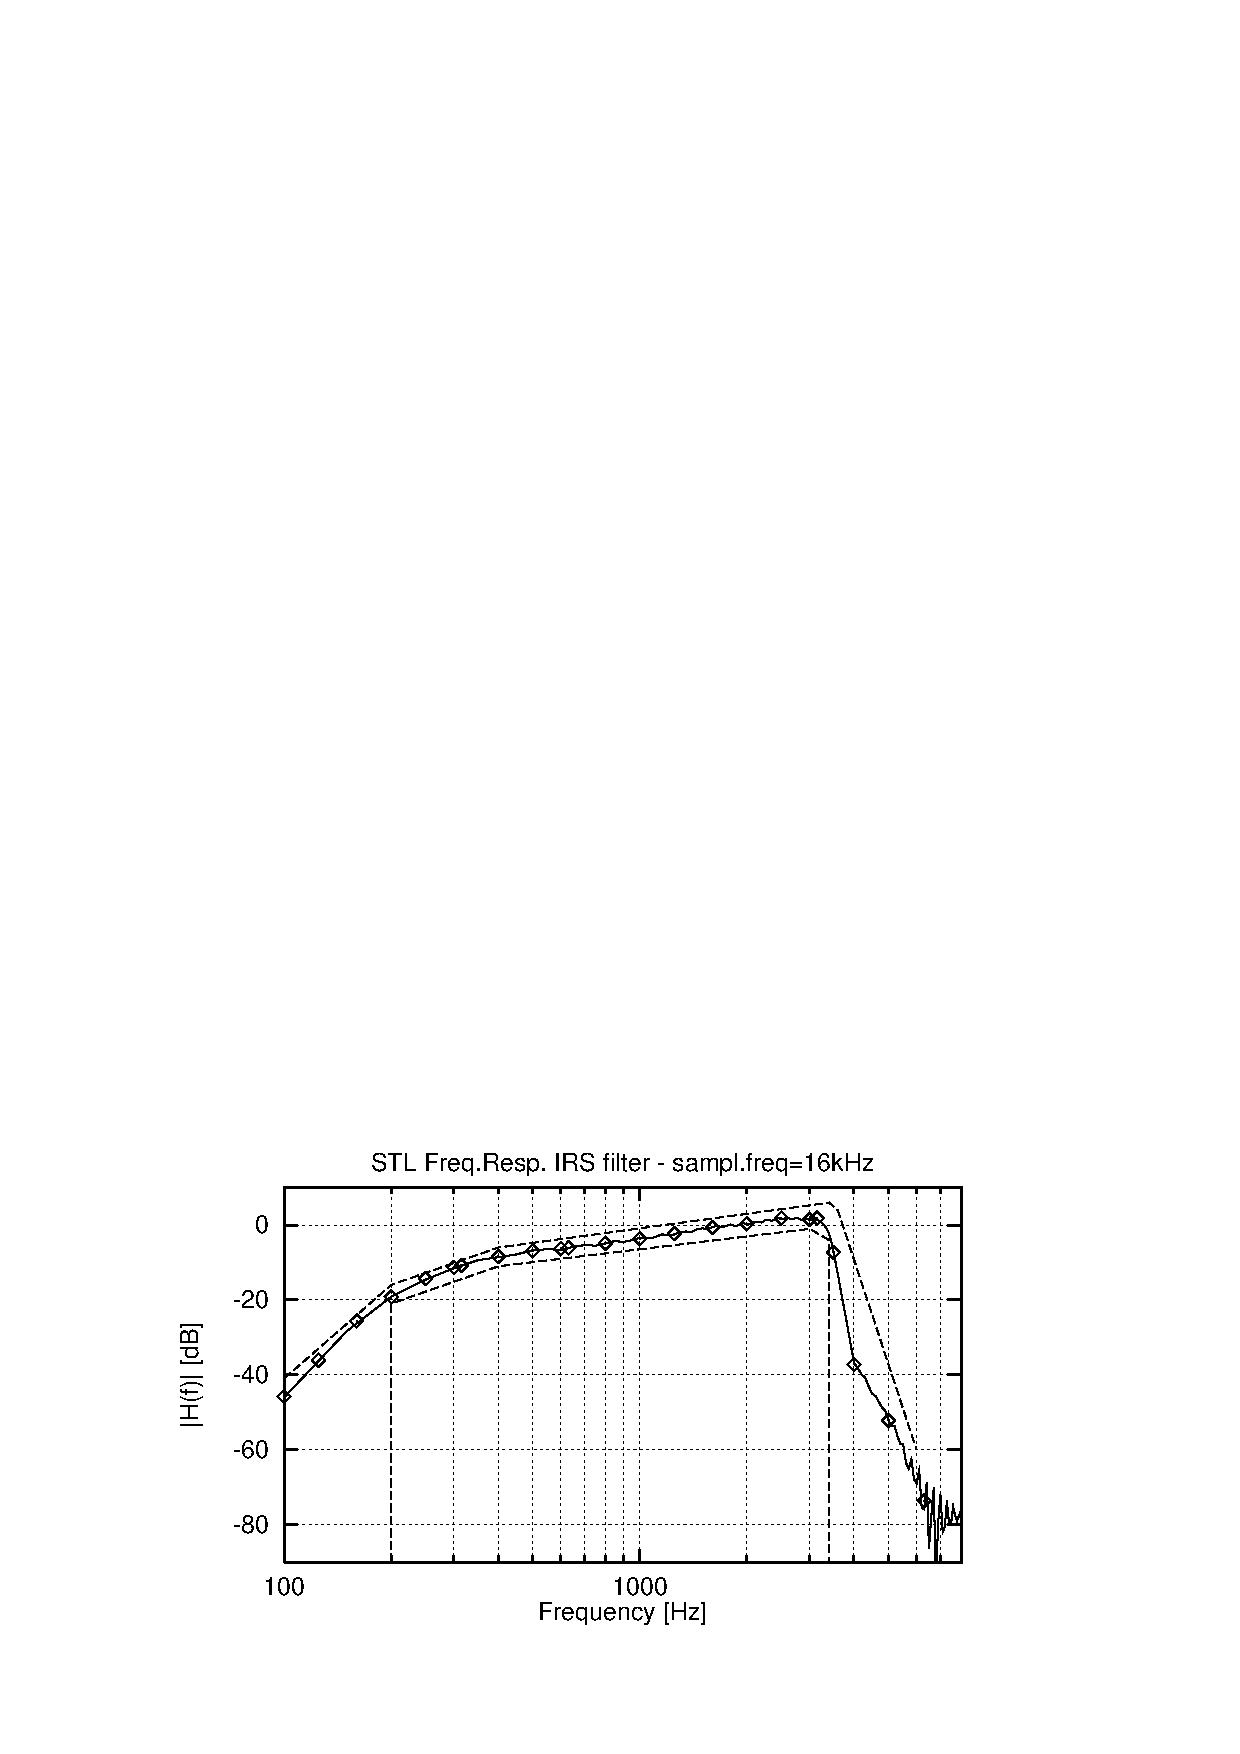
\includegraphics{irs_2_1}
    \\
   (b) Transmission-side IRS for input samples at 16 kHz.

  \end{center}
  \caption{\SF Transmission-side IRS filter responses.
               The diamonds represent the nominal values of the
               ``full'' IRS characteristic and the interrupted line
               represent the mask of the ``full'' IRS, as shown in
               figure 2 of ITU-T Rec. P.48.
               \label{tx-reg-irs-frq}}
\end{figure}
%------------------ End of regular IRS filters response ------------------


%-- Begin of FIR filters response: impulse response for regular IRS filters --
%Box dimension: 16.05cm x 18.03cm
\begin{figure}[hbtp]
  \begin{center}
     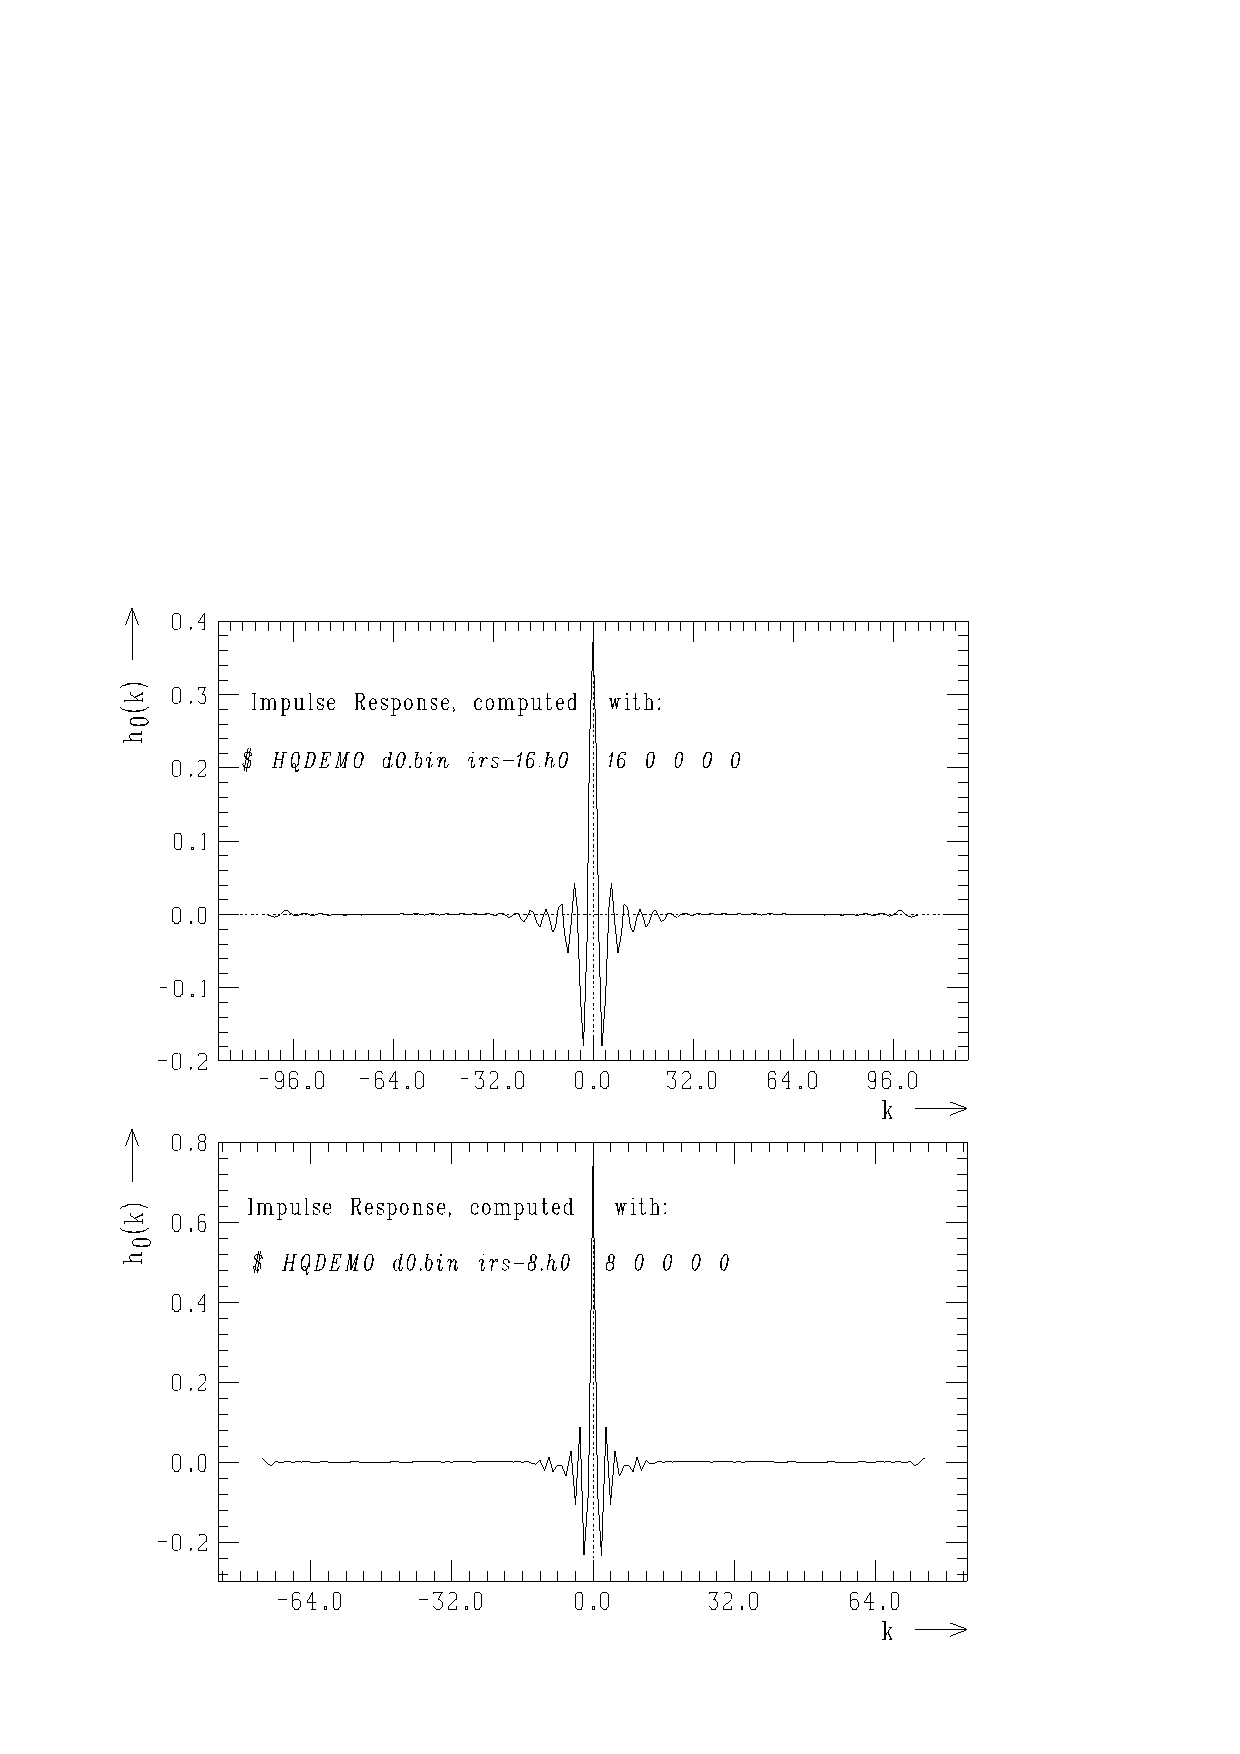
\includegraphics{irs-h0}
  \end{center}
  \caption{\SF Impulse response of transmission-side IRS filters
               at 16 and 8 kHz. \label{tx-reg-irs-ir}
          }
\end{figure}
%-- End of FIR filters response: impulse response for regular IRS filters --


%--------------- Begin of modified IRS TX filters response -----------------
\begin{figure}[hbtp]
  \begin{center}
     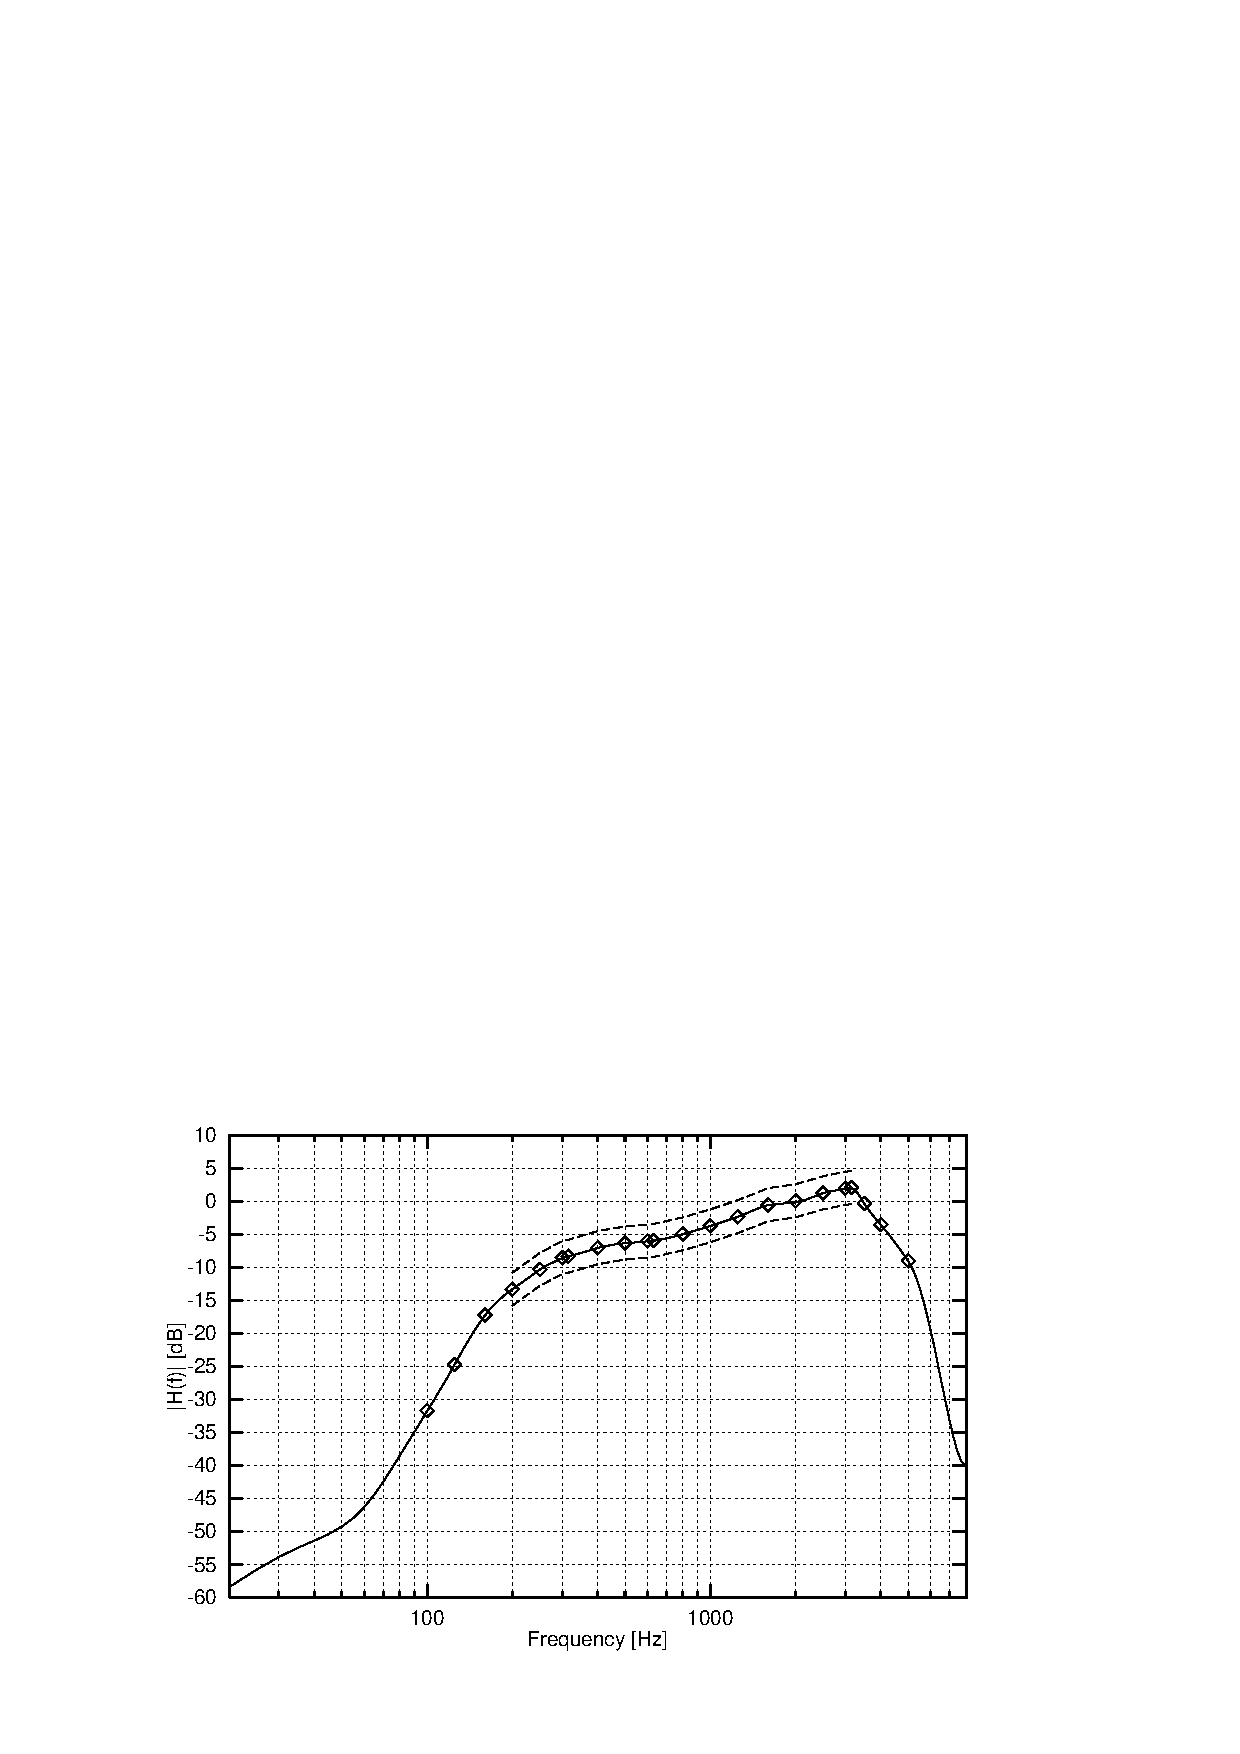
\includegraphics{mirs-16k}
     \\
   (a) Transmission-side modified IRS for input samples at 16 kHz.

     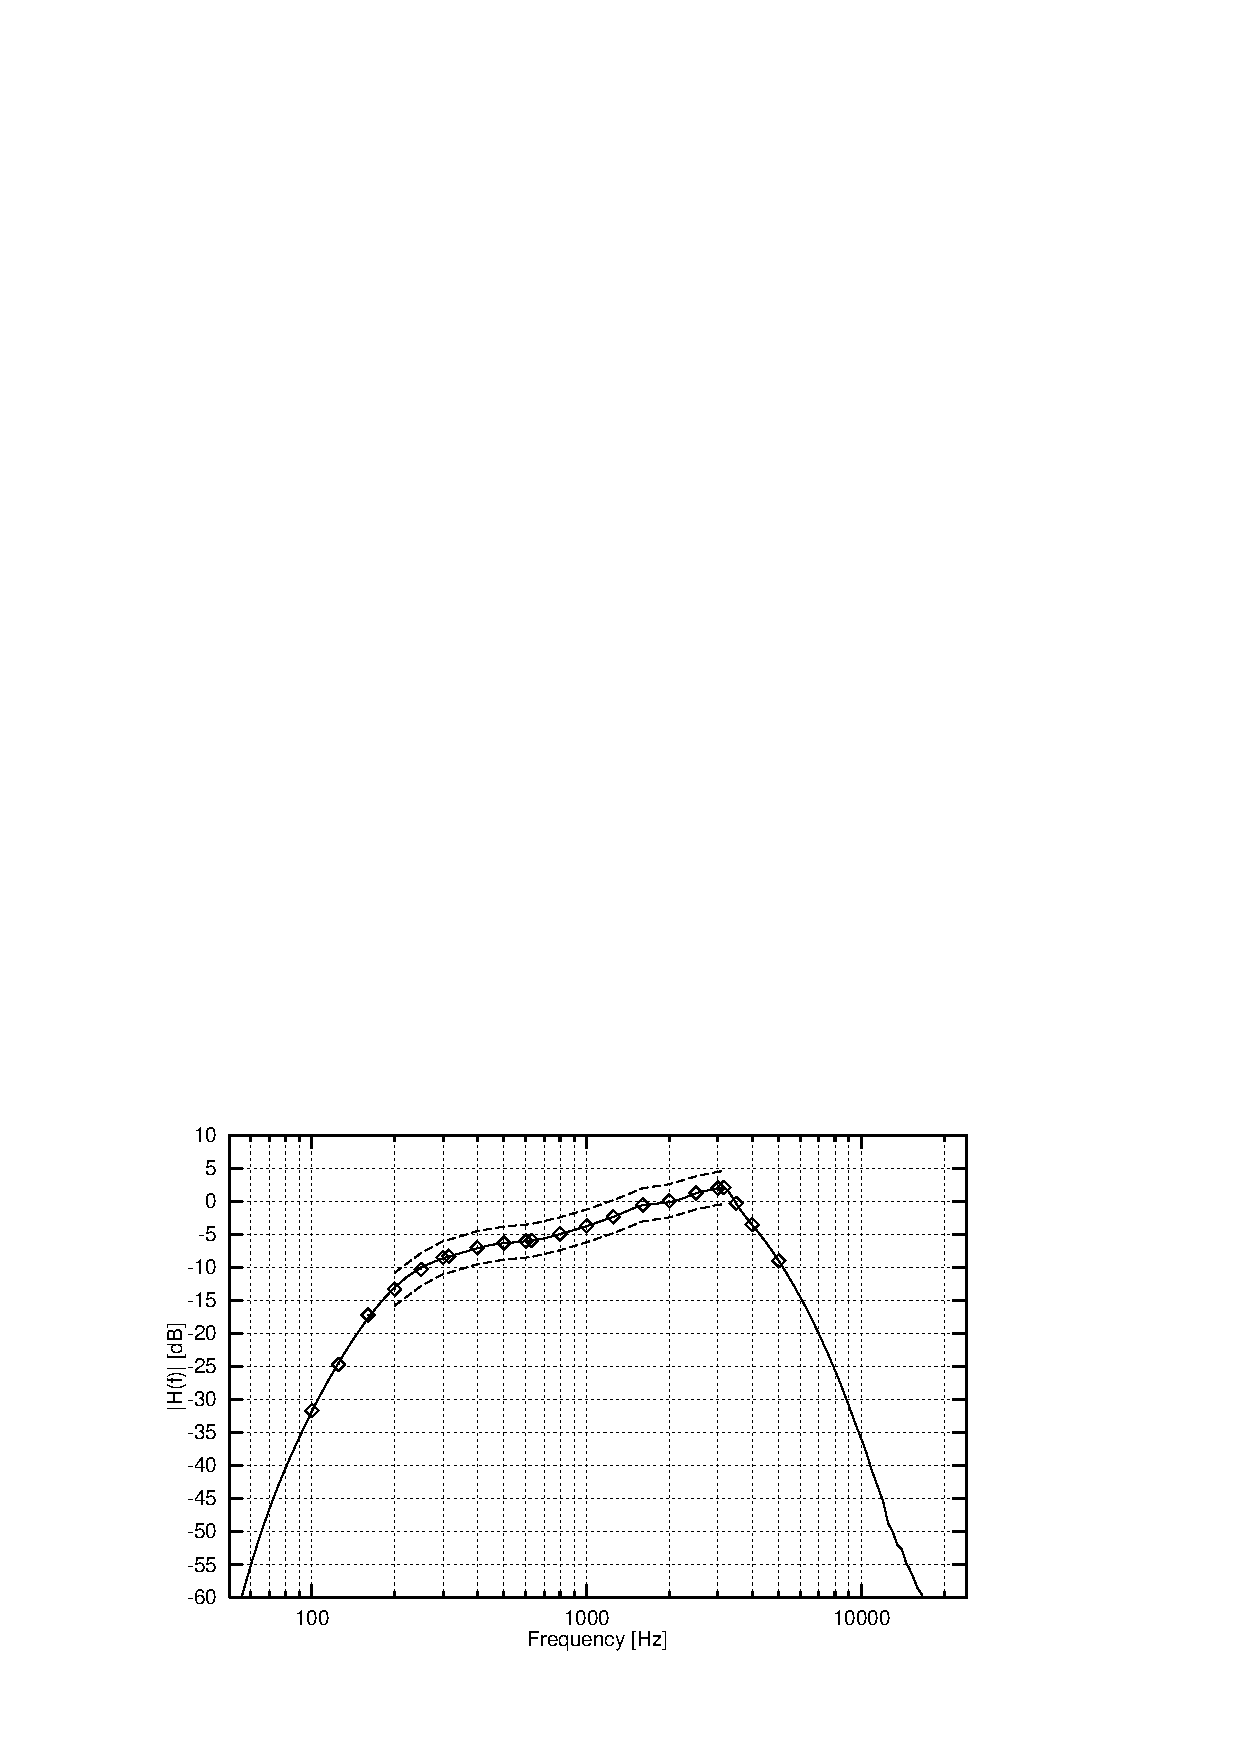
\includegraphics{mirs-48k}
    \\
   (b) Transmission-side modified IRS for input samples at 48 kHz.

  \end{center}
  \caption{\SF Transmission-side modified IRS filter responses. The
               interrupted line represents the mask of the ``full'' IRS.
               \label{tx-mod-irs-frq}}
\end{figure}
%------------------ End of modified IRS TX filters response -----------------


%-- Begin of FIR filters response: impulse response for mod IRS TX filters --
\begin{figure}[hbtp]
  \begin{center}
     \includegraphics{mirs16-h0}
    \\
   (a) Transmission-side modified IRS for input samples at 16 kHz.

     \includegraphics{mirs48-h0}
    \\
   (b) Transmission-side modified IRS for input samples at 48 kHz.

  \end{center}
  \caption{\SF Impulse response of transmission-side modified IRS filters
               at 16 kHz and 48 kHz. \label{tx-mod-irs-ir}
          }
\end{figure}
%----- End of FIR filters response: impulse response for IRS TX filters ------


%----------------- Begin of modified IRS RX filters response ----------------
\begin{figure}[hbtp]
  \begin{center}
    %Both boxes' dimension: 13.86cm x  7.30cm
     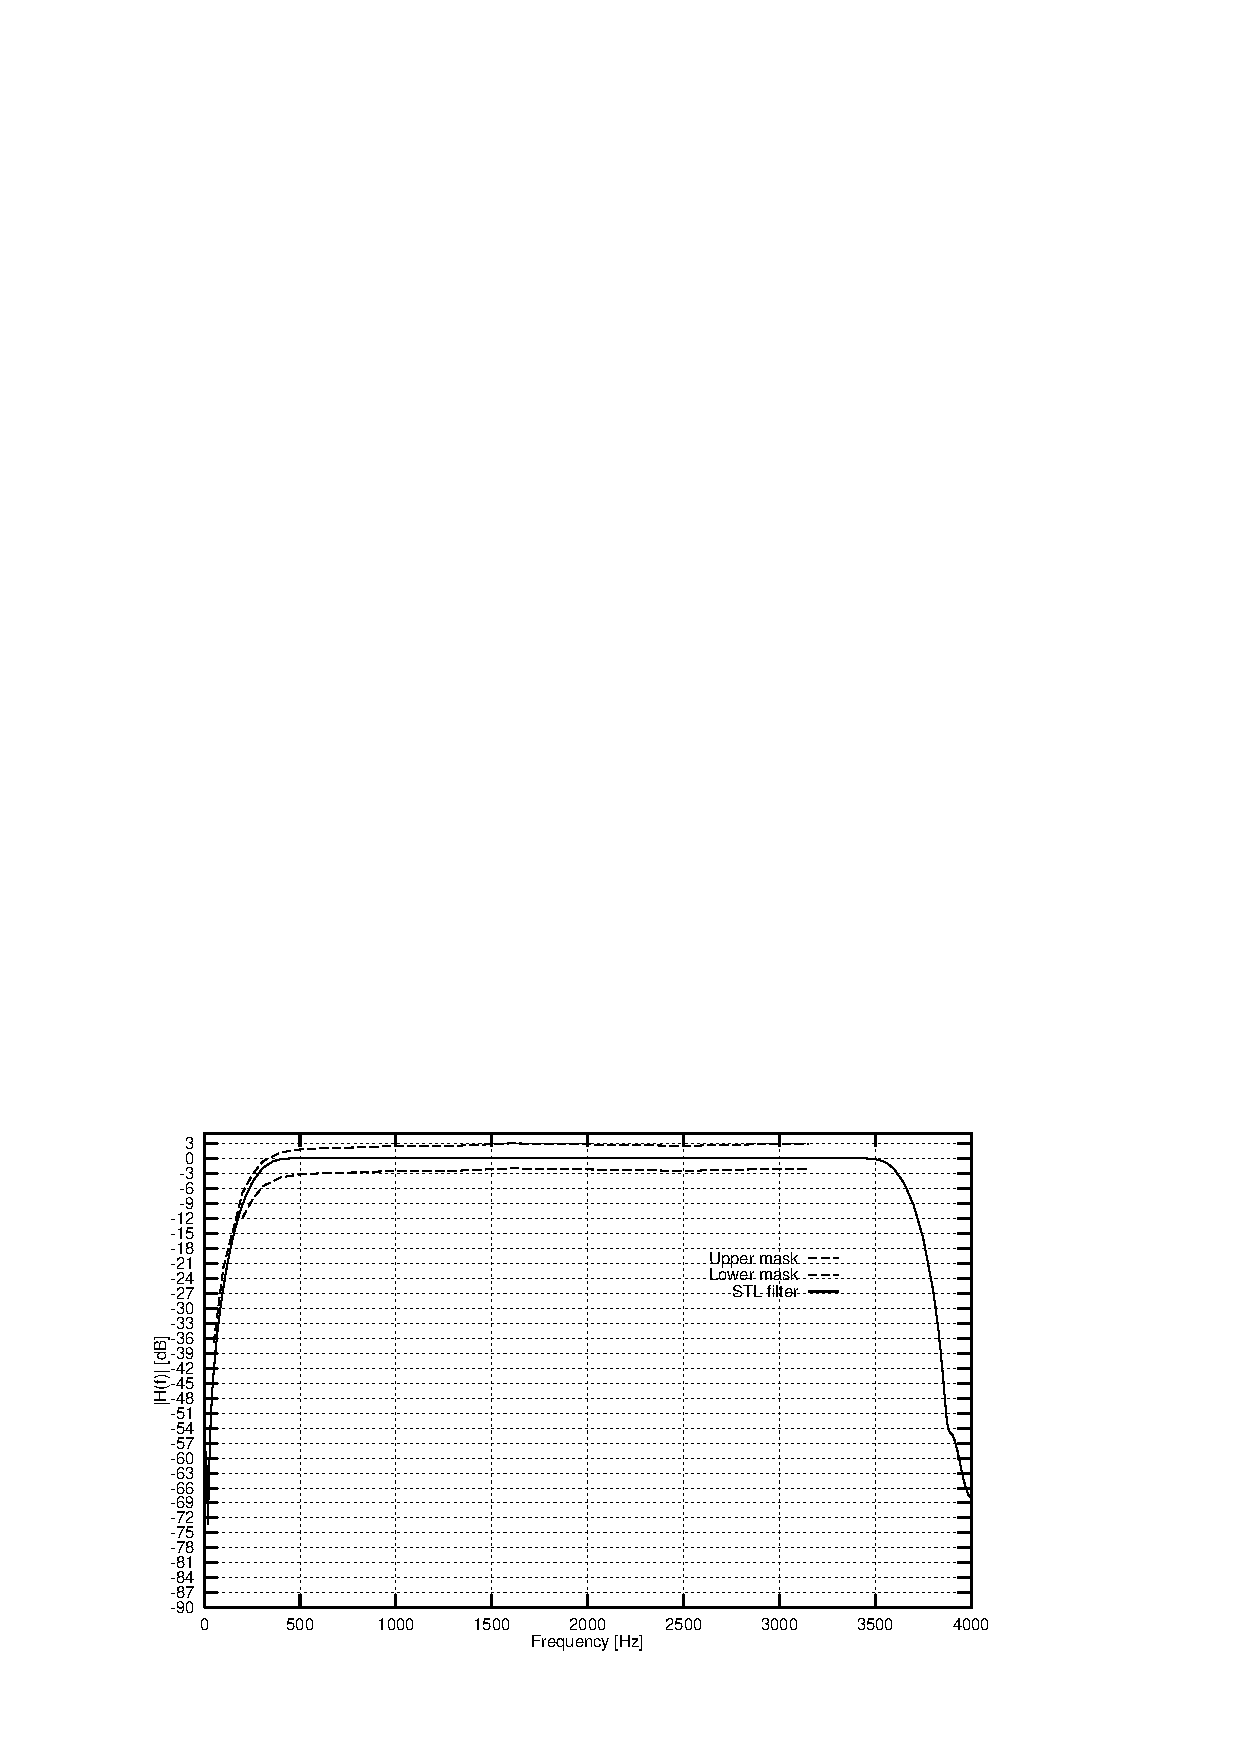
\includegraphics{rxirs08}
    \\
   (a) Receive-side modified IRS for input samples at 8 kHz.

     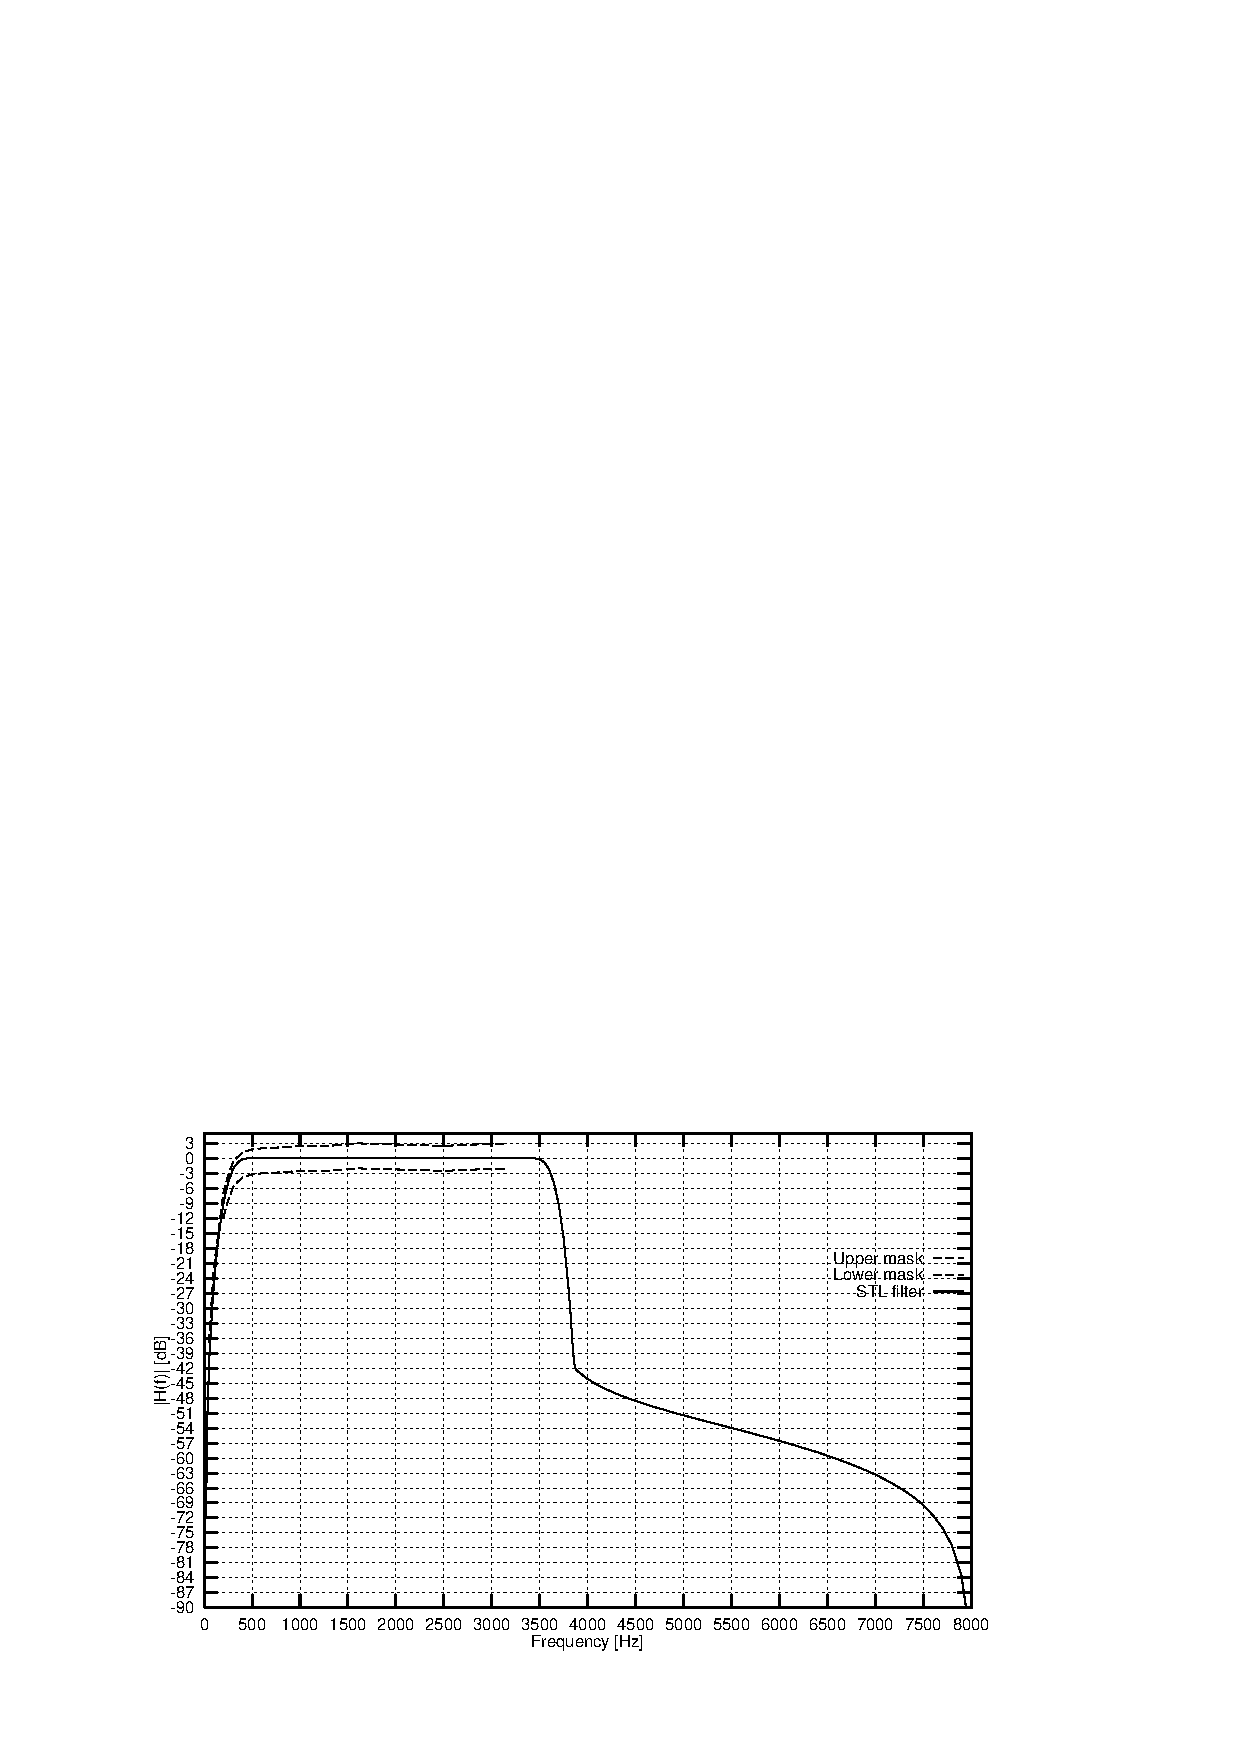
\includegraphics{rxirs16}
    \\
   (b) Receive-side modified IRS for input samples at 16 kHz.

  \end{center}
  \caption{\SF Receive-side modified IRS filter responses.
               The diamonds represent the nominal values of the
               modified IRS characteristic and the interrupted line
               represent the mask of the ``full'' IRS.
               \label{rx-mod-irs-frq}}
\end{figure}
%------------------ End of modified IRS RX filters response ----------------

\flushfloats
%-- Begin of FIR filters response: impulse response for mod IRS RX filters --
\begin{figure}[hbtp]
  \begin{center}
     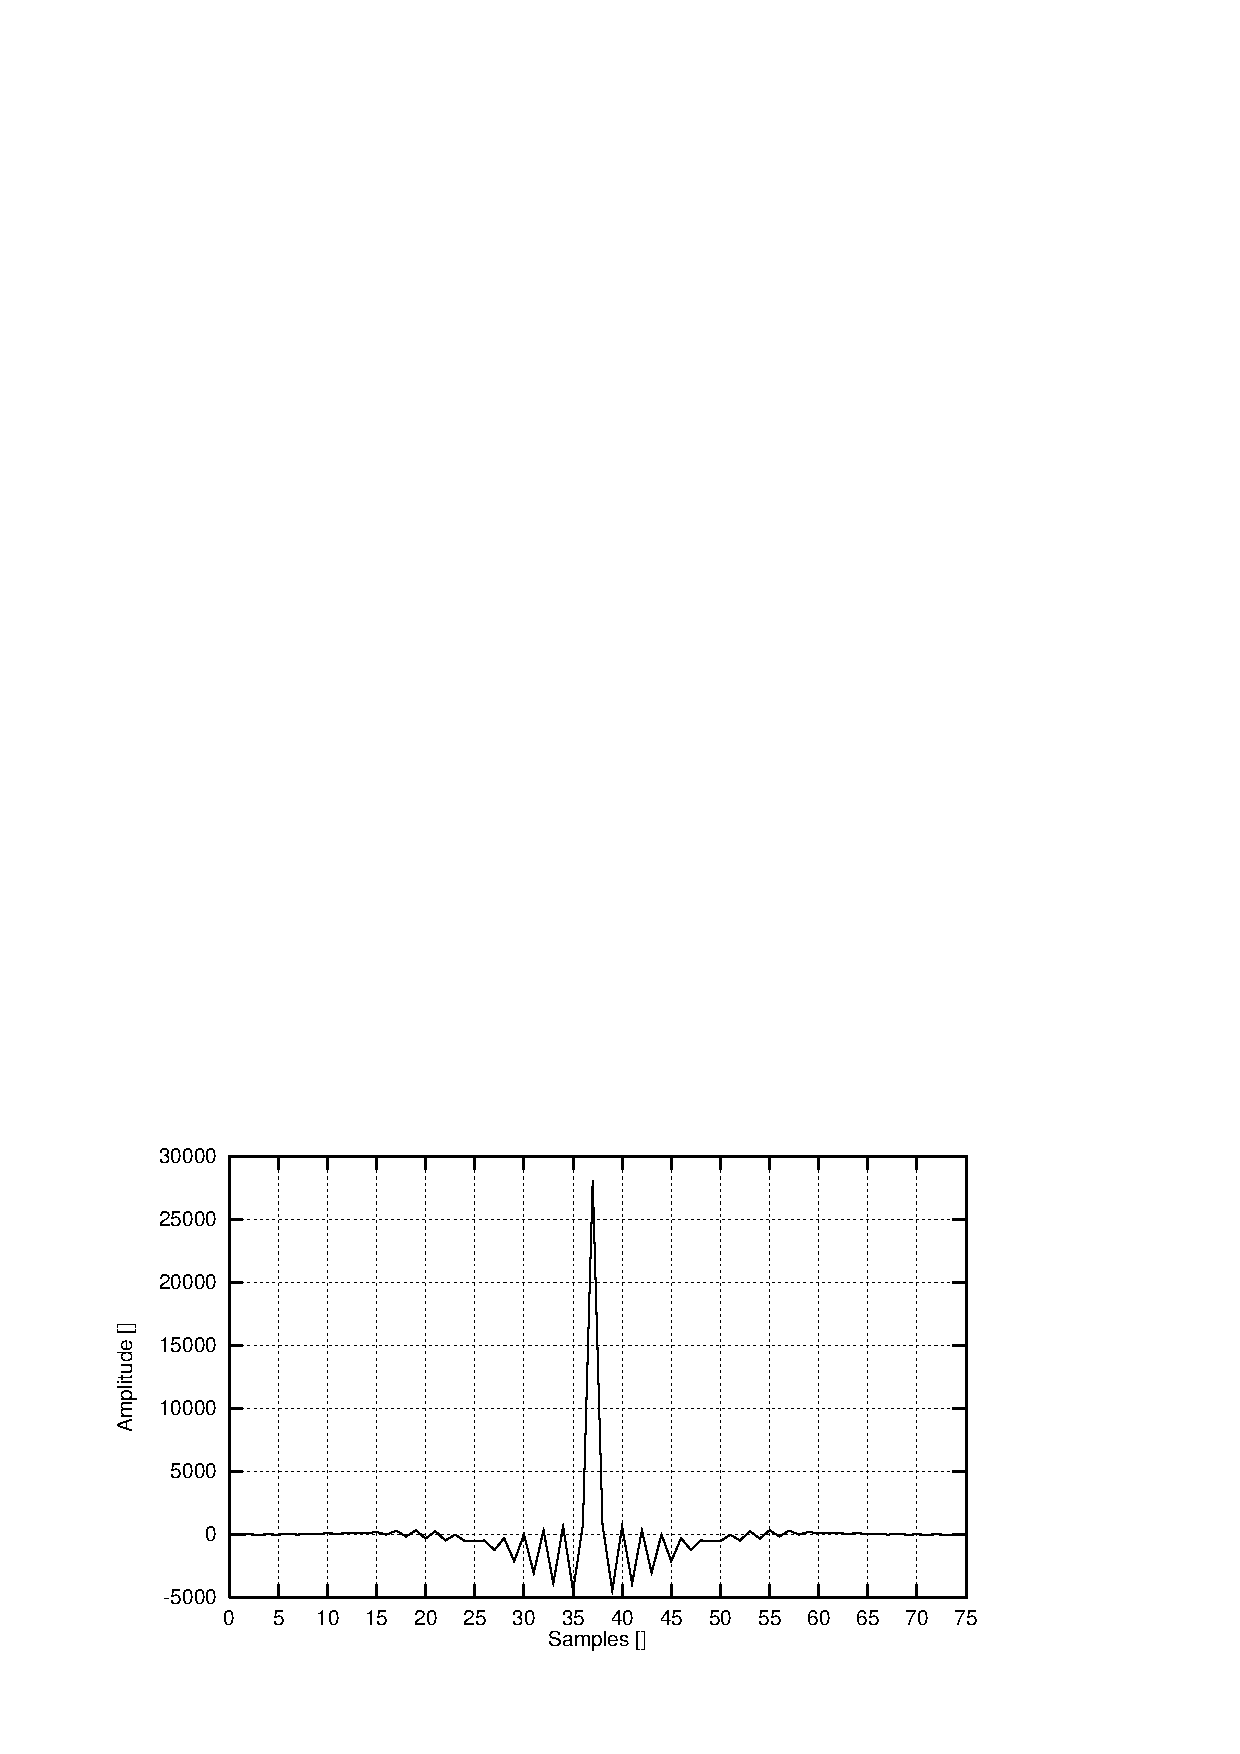
\includegraphics{rxirs08-h0}
    \\
   (a) Receive-side modified IRS for input samples at 8 kHz.

     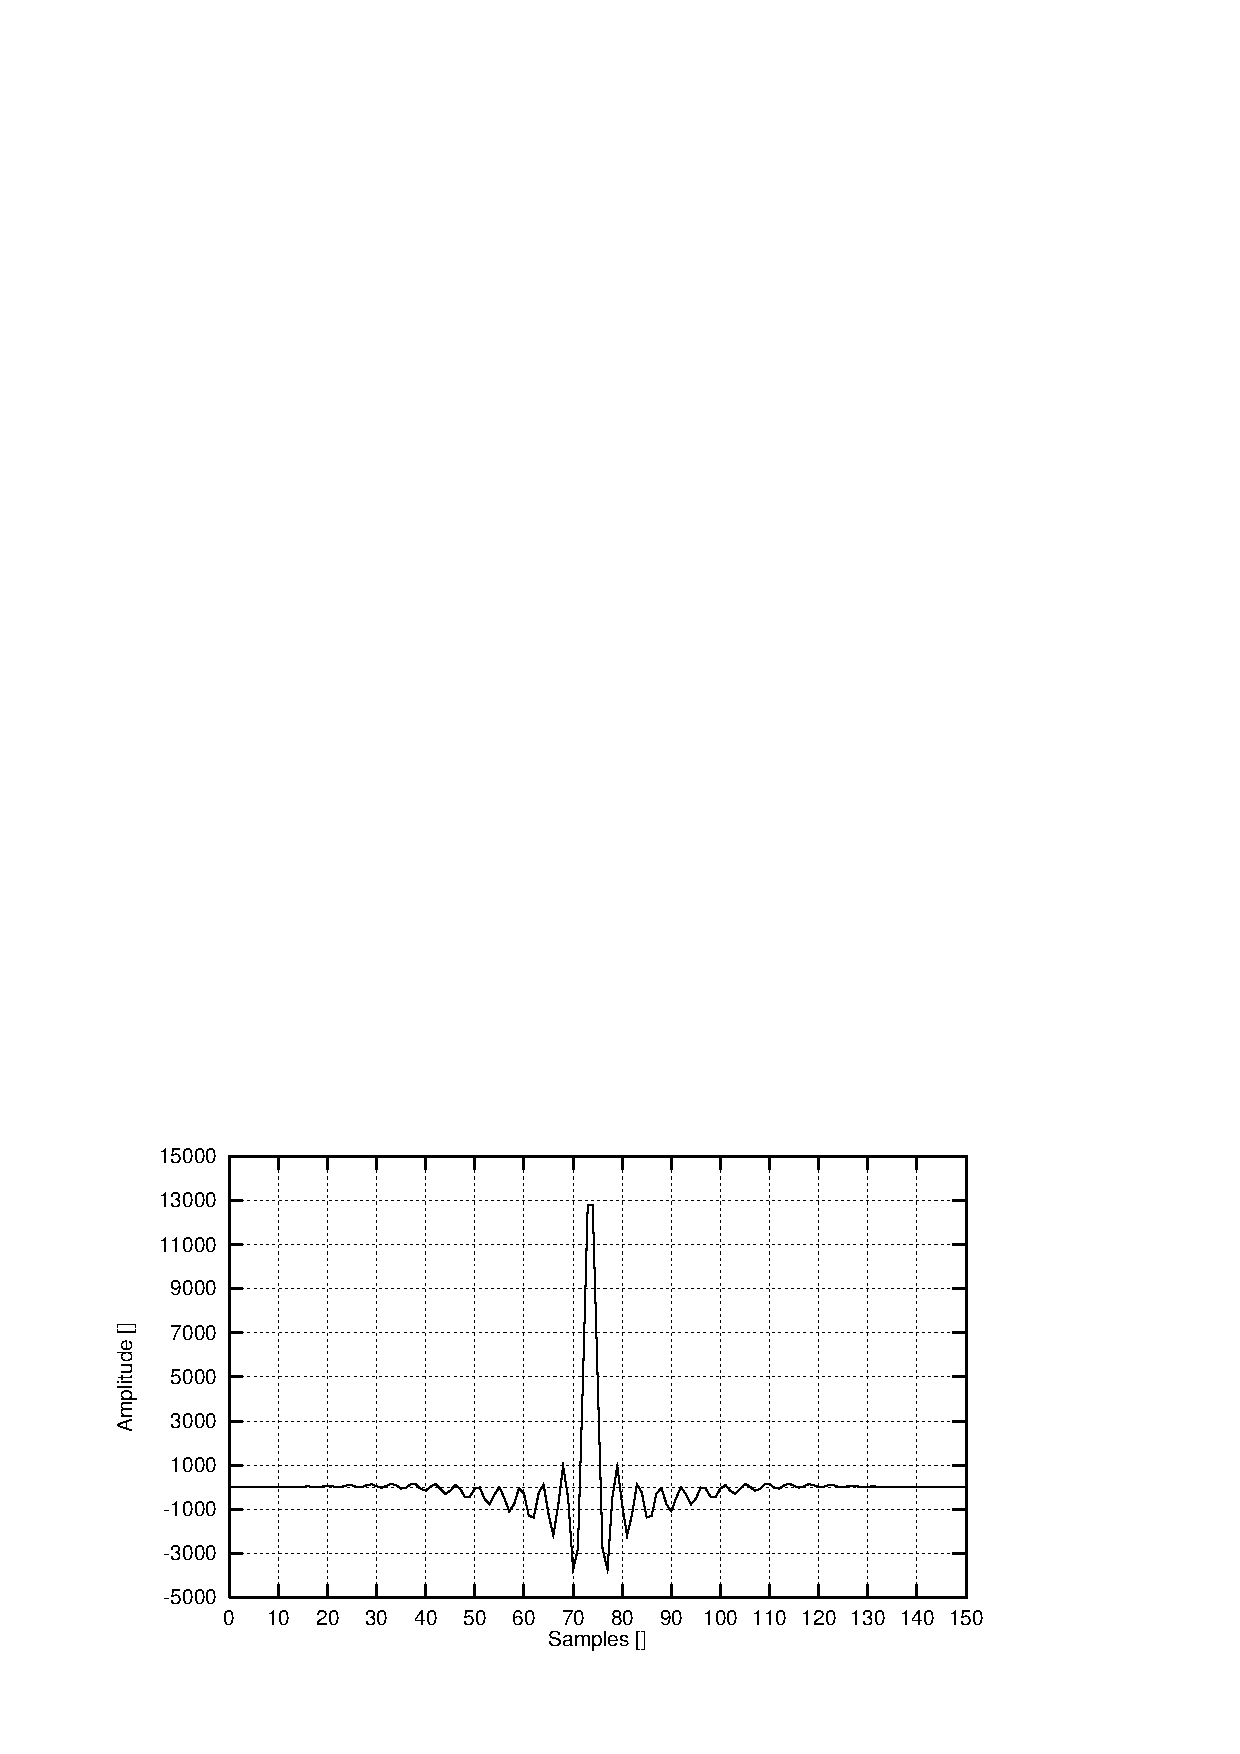
\includegraphics{rxirs16-h0}
    \\
   (b) Receive-side modified IRS for input samples at 16 kHz.

  \end{center}
  \caption{\SF Impulse response of receive-side modified IRS filters at 8 kHz
               (top) and 16 kHz (bottom). \label{rx-mod-irs-ir}
          }
\end{figure}
%--- End of FIR filters response: impulse response for RX mod IRS filters ---


%----------- Begin of FIR filters response: frq for psophometric filter  ----
\begin{figure}[hbtp]
  \begin{center}
 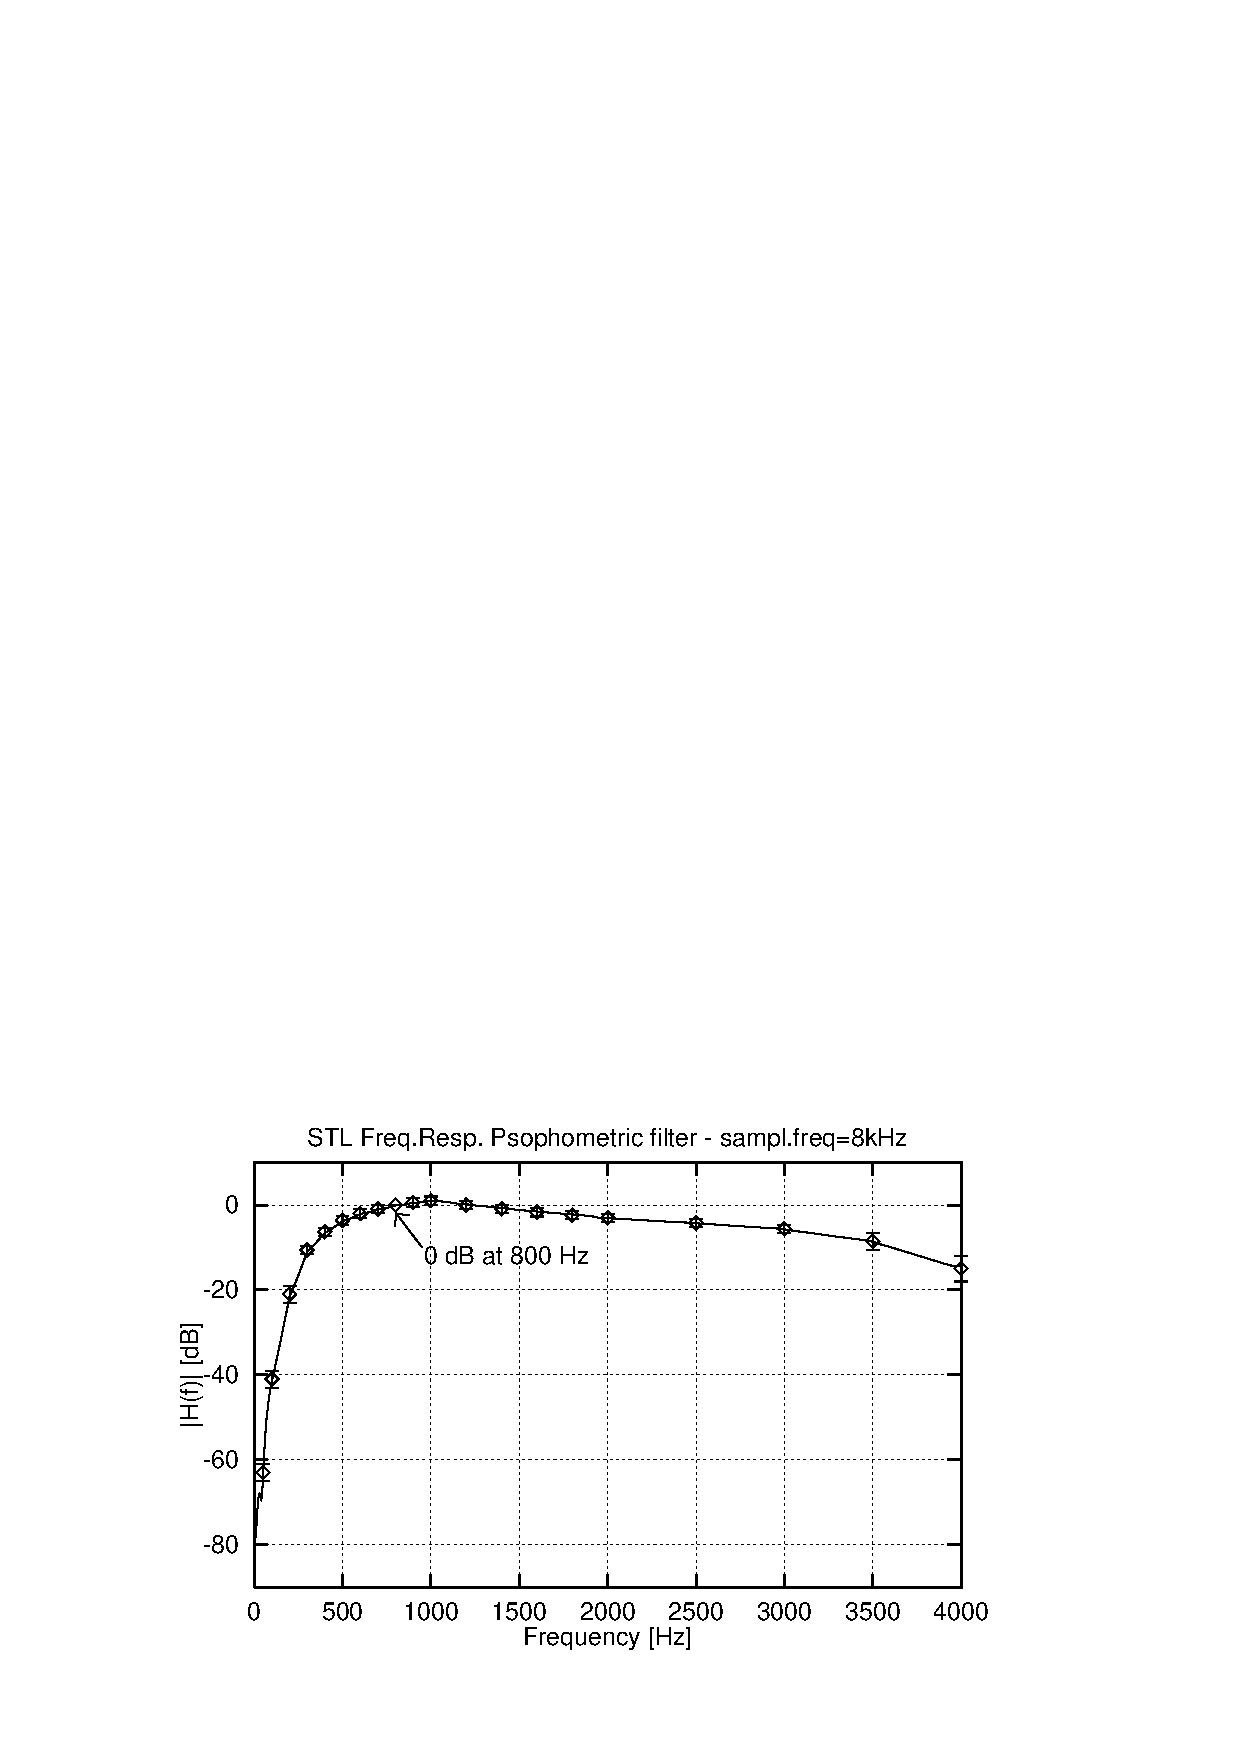
\includegraphics{pso_8k}
  \end{center}
  \caption{\SF Frequency response for the psophometric filter. The
               points show the average points and the allowed range as per
               ITU-T Rec. O.41.
               \label{pso-08k-frq}
          }

\end{figure}
%------------- End of FIR filters response: frq for psophometric -------------


%----------- Begin of FIR filters response: frq for deltasm filter  ----
\begin{figure}[hbtp]
  \begin{center}
 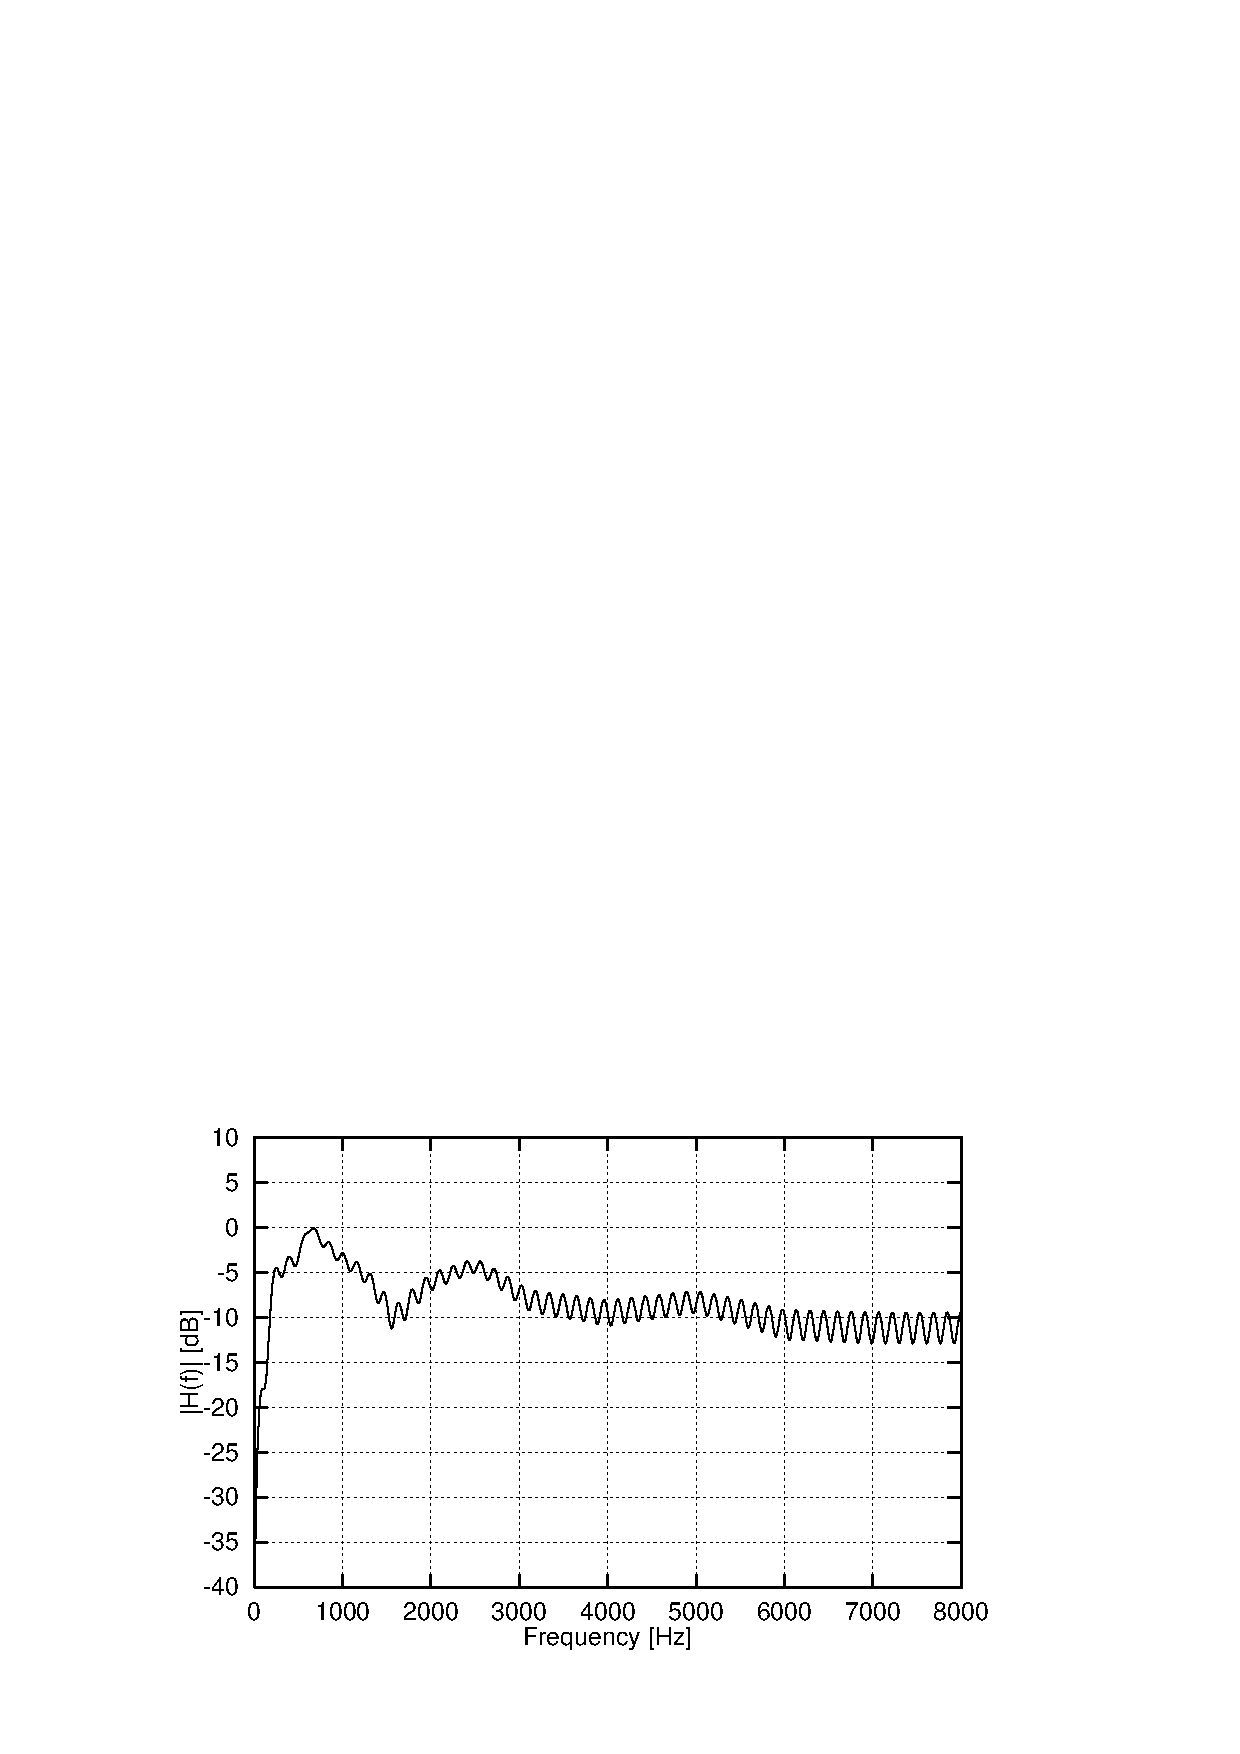
\includegraphics{dsm_16k}

  \end{center}
  \caption{\SF Frequency response for the $\Delta_{SM}$ filter.
               \label{delta-sm-frq}
          }

\end{figure}
%------------- End of FIR filters response: frq for deltasm -------------


%----------- Begin of FIR filters response: frq for P.341 filter  --------
\begin{figure}[hbtp]
  \begin{center}
 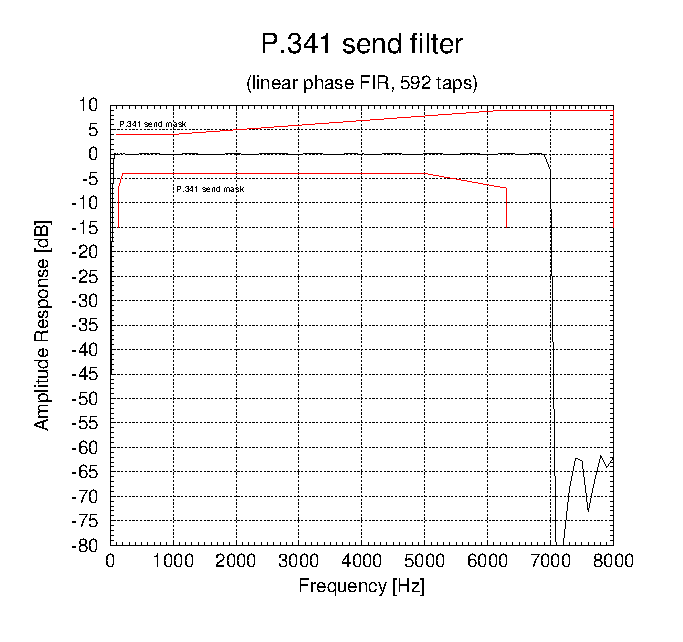
\includegraphics{p341}
  \end{center}
  \caption{\SF STL P.341 send-side filter frequency response for data
               sampled at 16 kHz (factor 1:1).
           \label{tx-p341-frq}
          }
\end{figure}
%------------- End of FIR filters response: frq for P.341 ----------------


%--- Begin of FIR filters response: impulse response for P.341 --------
\begin{figure}[hbtp]
  \begin{center}
 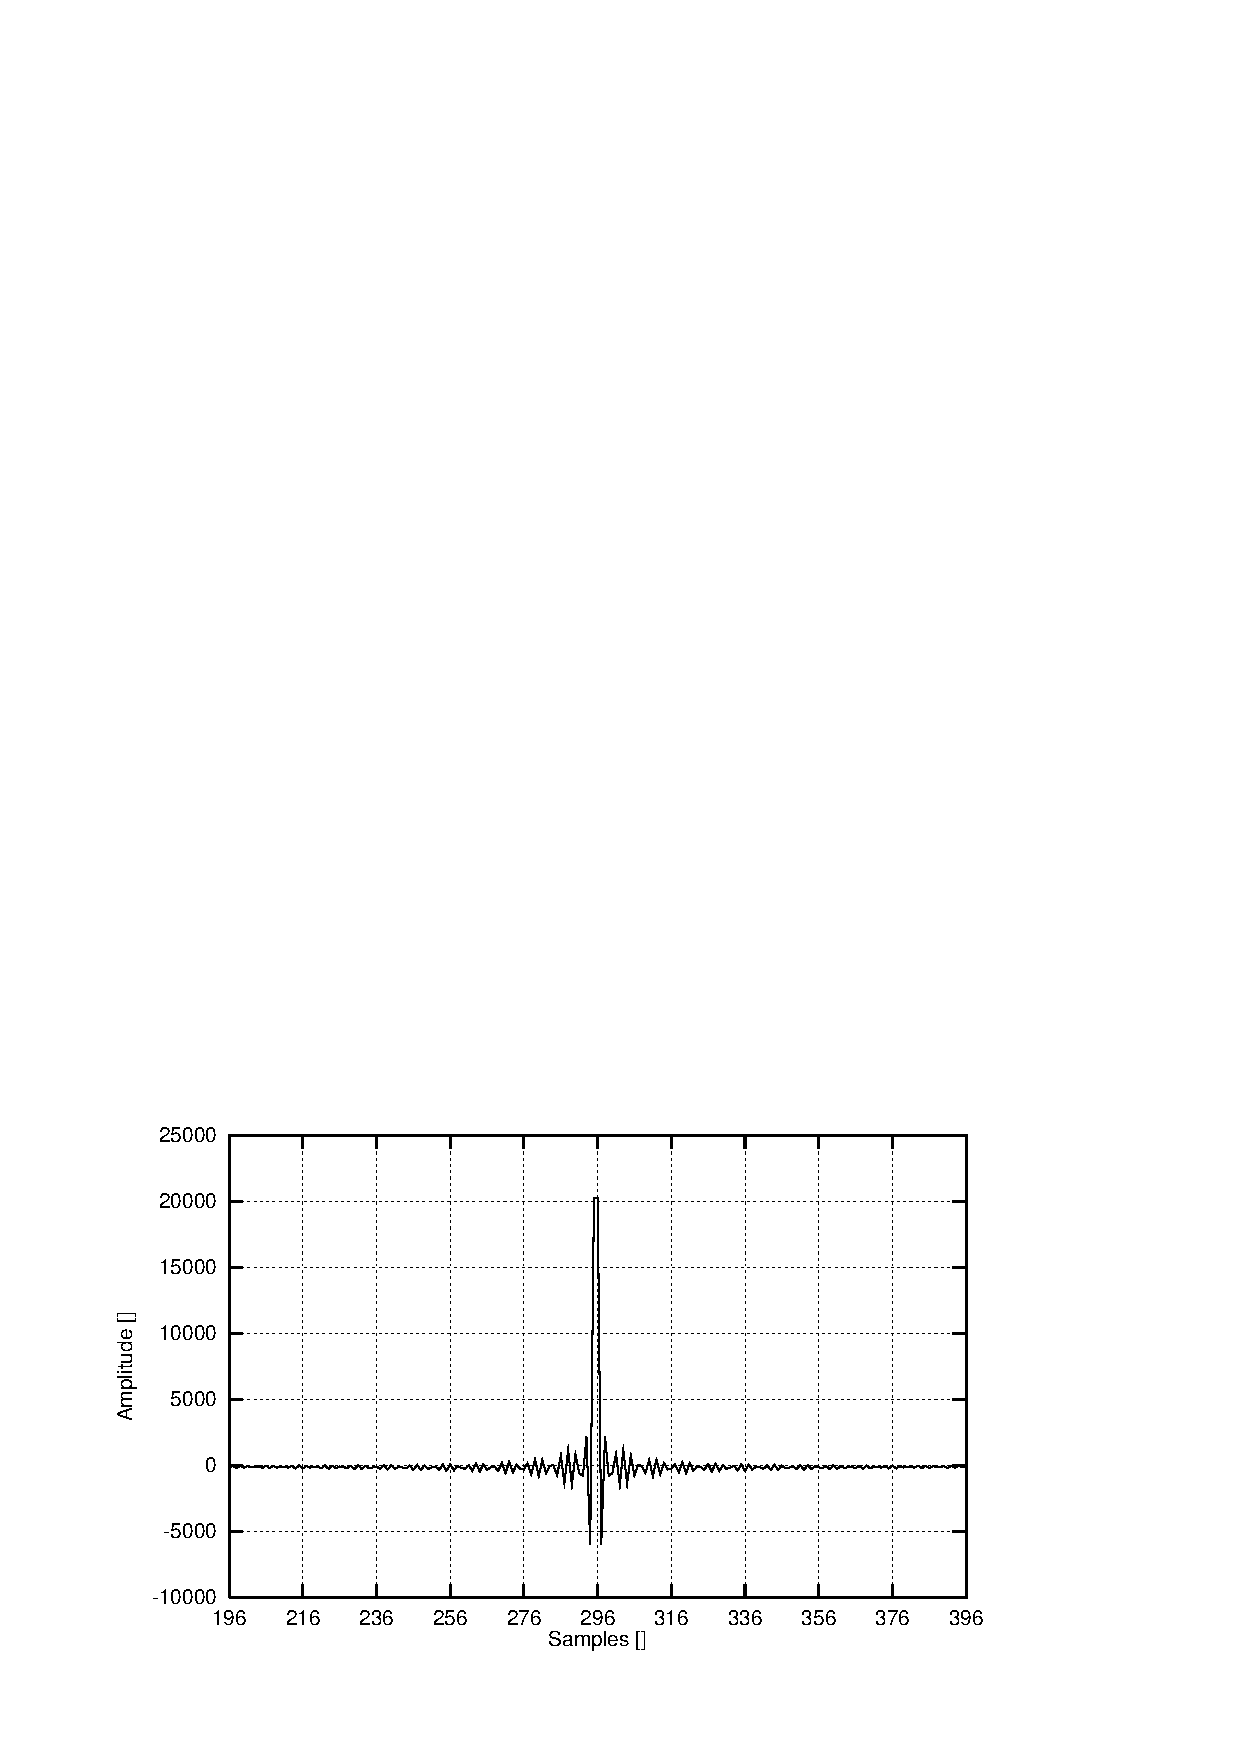
\includegraphics{p341-h0}
  \end{center}
  \caption{\SF STL P.341 send-side filter impulse response.
           \label{tx-p341-ir}
          }
\end{figure}
%----- End of FIR filters response: impulse response for P.341 -----


%----------- Begin of FIR filters response: frq for 50 Hz-14 kHz BP filter  ----
\begin{figure}[hbtp]
  \begin{center}
  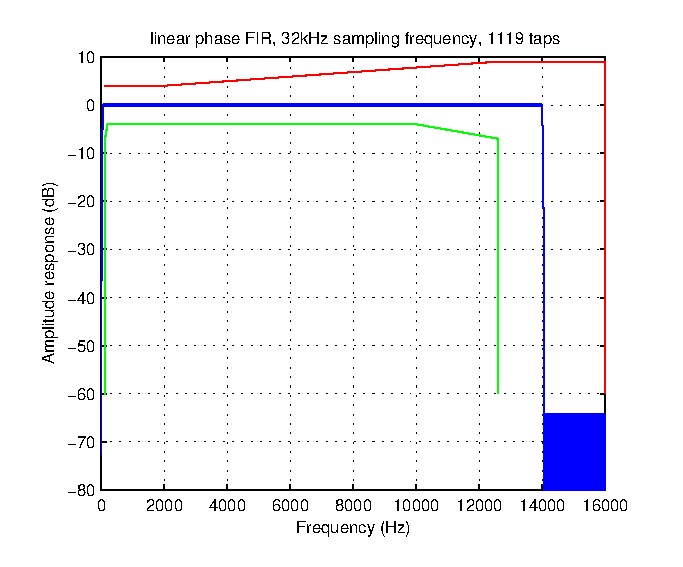
\includegraphics{50-14K}
  \end{center}
  \caption{\SF STL 50 Hz - 14 kHz band limiting filter frequency response for data
               sampled at 32 kHz (factor 1:1).
           \label{50_14k-32k-frq}
          }
\end{figure}
%------------- End of FIR filters response: frq for 50 Hz-14 kHz BP -------------


%--- Begin of FIR filters response: impulse response for 50 Hz - 14 kHz BP --------
\begin{figure}[hbtp]
  \begin{center}
 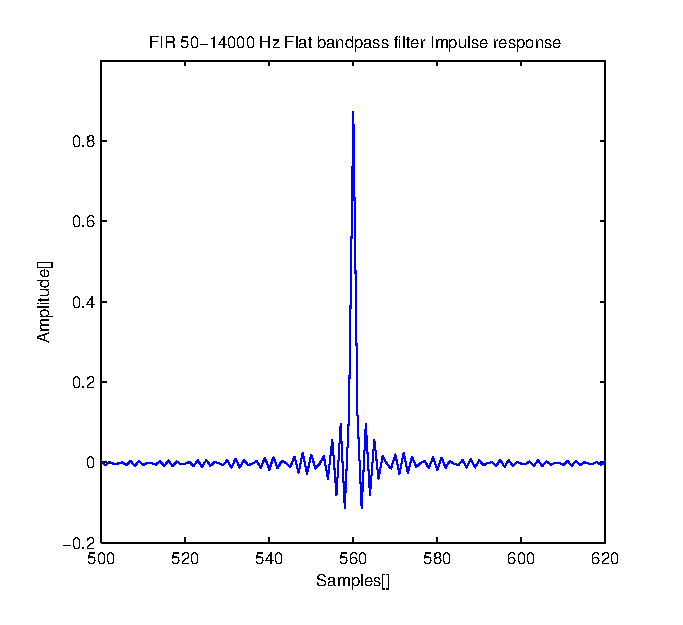
\includegraphics{50-14K-h0}
  \end{center}
  \caption{\SF STL 50 Hz - 14 kHz band limiting filter impulse response.
           \label{50_14k-32k-ir}
          }
\end{figure}
%----- End of FIR filters response: impulse response for 50 Hz - 14 kHz BP -----

\clearpage
\newpage


%%PROBLEM
%----------- Begin of FIR filters response: frq for 50 Hz - 5 kHz BP filter  ----
\begin{figure}[hbtp]
  \begin{center}
 \includegraphics{bp5k}

  \end{center}
  \caption{\SF STL 50 Hz - 5 kHz band limiting filter frequency response for data
               sampled at 16 kHz (factor 1:1).
           \label{bp5k-16k-frq}
          }
\end{figure}
%------------- End of FIR filters response: frq for 50 Hz - 5 kHz BP -------------


%--- Begin of FIR filters response: impulse response for 50 Hz - 5 kHz BP --------
\begin{figure}[h!btp]
  \begin{center}
 \includegraphics{bp5k-h0}
  \end{center}
  \caption{\SF STL 50 Hz - 5 kHz band limiting filter impulse response.
           \label{bp5k-16k-ir}
          }
\end{figure}
%----- End of FIR filters response: impulse response for 50 Hz - 5 kHz BP -----


%----------- Begin of FIR filters response: frq for 100 Hz - 5 kHz BP filter  ----
\begin{figure}[hbtp]
  \begin{center}
 \includegraphics{bp100_5k}
  \end{center}
  \caption{\SF STL 100 Hz - 5 kHz band limiting filter frequency response for data
               sampled at 16 kHz (factor 1:1).
           \label{bp100_5k-16k-frq}
          }
\end{figure}
%------------- End of FIR filters response: frq for 100 Hz - 5 kHz BP -------------


%--- Begin of FIR filters response: impulse response for 100 Hz - 5 kHz BP --------
\begin{figure}[hbtp]
  \begin{center}
 \includegraphics{bp100_5k-h0}
  \end{center}
  \caption{\SF STL 100 Hz - 5 kHz band limiting filter impulse response.
           \label{bp100_5k-16k-ir}
          }
\end{figure}
%----- End of FIR filters response: impulse response for 100 Hz-5 kHz BP -----


%----------- Begin of FIR filters response: frq for 20 Hz - 20 kHz BP filter  ----
\begin{figure}[h]
  \begin{center}
\includegraphics[scale=0.7]{bp20_20k}
  \end{center}
  \caption{\SF STL 20 Hz - 20 kHz band limiting filter frequency response for data
               sampled at 48 kHz (factor 1:1).
           \label{bp20_20k-48k-frq}
          }
\end{figure}
%------------- End of FIR filters response: frq for 20 Hz - 20 kHz BP -------------


%--- Begin of FIR filters response: impulse response for 20 Hz - 20 kHz BP --------
\begin{figure}[b]
  \begin{center}
 \includegraphics[scale=0.7]{bp20_20k-h0}
  \end{center}
  \caption{\SF STL 20 Hz - 20 kHz band limiting filter impulse response, (the complete impulse response is of length 4001).
           \label{bp20_20k-48k-ir}
          }
\end{figure}
%----- End of FIR filters response: impulse response for 20 Hz - 20 kHz BP -----


%----------- Begin of FIR filters response: frq for LP1p5 filter  ----
\begin{figure}[hbtp]
  \begin{center}
 \includegraphics[scale=0.65]{LP1p5}
  \end{center}
  \caption{\SF Frequency response of the STL MUSHRA anchor LP1.5 -- Low-pass filter with cut-off frequency 1.5 kHz for a sampling frequency of 48 kHz (factor 1:1).
           \label{LP1p5-frq}
          }
\end{figure}
%------------- End of FIR filters response: frq for LP1p5 -------------

%--- Begin of FIR filters response: impulse response for LP1p5 --------
\begin{figure}[hbtp]
  \begin{center}
 \includegraphics[scale=0.65]{LP1p5-h0}
  \end{center}
  \caption{\SF Impulse response of the STL MUSHRA anchor LP1.5 -- Low-pass filter with cut-off frequency 1.5 kHz for a sampling frequency of 48 kHz (factor 1:1).
           \label{LP1p5-ir}
          }
\end{figure}
%----- End of FIR filters response: impulse response for LP1p5 -----


%----------- Begin of FIR filters response: frq for LP35 filter  ----
\begin{figure}[hbtp]
  \begin{center}
 \includegraphics{LP35}
  \end{center}
  \caption{\SF Frequency response of the STL MUSHRA anchor LP3.5 -- Low-pass filter with cut-off frequency 3.5 kHz for a sampling frequency of 48 kHz (factor 1:1).
           \label{LP35-frq}
          }
\end{figure}
%------------- End of FIR filters response: frq for LP35 -------------

%--- Begin of FIR filters response: impulse response for LP35 --------
\begin{figure}[hbtp]
  \begin{center}
 \includegraphics{LP35-h0}
  \end{center}
  \caption{\SF Impulse response of the STL MUSHRA anchor LP3.5 -- Low-pass filter with cut-off frequency 3.5 kHz for a sampling frequency of 48 kHz (factor 1:1).
           \label{LP35-ir}
          }
\end{figure}
%----- End of FIR filters response: impulse response for LP35 -----


%----------- Begin of FIR filters response: frq for LP7 filter  ----
\begin{figure}[hbtp]
  \begin{center}
 \includegraphics{LP7}
  \end{center}
  \caption{\SF Frequency response of the STL MUSHRA anchor LP7 -- Low-pass filter with cut-off frequency 7 kHz for a sampling frequency of 48 kHz (factor 1:1).
           \label{LP7-frq}
          }
\end{figure}
%------------- End of FIR filters response: frq for LP7 -------------


%--- Begin of FIR filters response: impulse response for LP7 --------
\begin{figure}[hbtp]
  \begin{center}
 \includegraphics{LP7-h0}
  \end{center}
  \caption{\SF Impulse response of the STL MUSHRA anchor LP7 -- Low-pass filter with cut-off frequency 7 kHz for a sampling frequency of 48 kHz (factor 1:1).
           \label{LP7-ir}
          }
\end{figure}
%----- End of FIR filters response: impulse response for LP7 -----


%----------- Begin of FIR filters response: frq for LP10 filter  ----
\begin{figure}[hbtp]
  \begin{center}
 \includegraphics{LP10}
  \end{center}
  \caption{\SF Frequency response of the STL MUSHRA anchor LP10 -- Low-pass filter with cut-off frequency 10 kHz for a sampling frequency of 48 kHz (factor 1:1).
           \label{LP10-frq}
          }
\end{figure}
%------------- End of FIR filters response: frq for LP10 -------------


%--- Begin of FIR filters response: impulse response for LP10 --------
\begin{figure}[hbtp]
  \begin{center}
 \includegraphics{LP10-h0}
  \end{center}
  \caption{\SF Impulse response of the STL MUSHRA anchor LP10 -- Low-pass filter with cut-off frequency 10 kHz for a sampling frequency of 48 kHz (factor 1:1).
           \label{LP10-ir}
          }
\end{figure}
%----- End of FIR filters response: impulse response for LP10 -----

%----------- Begin of FIR filters response: frq for LP12 filter  ----
\begin{figure}[hbtp]
  \begin{center}
% \includegraphics{LP12-h0}
 \includegraphics[angle=-90,scale=0.7]{LP12-h0new}
  \end{center}
  \caption{\SF Frequency response of the STL MUSHRA anchor LP12 -- Low-pass filter with cut-off frequency 12 kHz for a sampling frequency of 48 kHz (factor 1:1).
           \label{LP12-frq}
          }
\end{figure}
%------------- End of FIR filters response: frq for LP12 -------------


%--- Begin of FIR filters response: impulse response for LP12 --------
\begin{figure}[hbtp]
  \begin{center}
% \includegraphics{LP12}
 \includegraphics[angle=-90,scale=0.7]{LP12new}
  \end{center}
  \caption{\SF Impulse response of the STL MUSHRA anchor LP12 -- Low-pass filter with cut-off frequency 12 kHz for a sampling frequency of 48 kHz (factor 1:1).
           \label{LP12-ir}
          }
\end{figure}
%----- End of FIR filters response: impulse response for LP12 -----


%----------- Begin of FIR filters response: frq for LP14 filter  ----
\begin{figure}[hbtp]
  \begin{center}
 \includegraphics[scale=0.6]{LP14}
  \end{center}
  \caption{\SF Frequency response of the STL MUSHRA anchor LP14 -- Low-pass filter with cut-off frequency 14 kHz for a sampling frequency of 48 kHz (factor 1:1).
           \label{LP14-frq}
          }
\end{figure}
%------------- End of FIR filters response: frq for LP14 -------------

%--- Begin of FIR filters response: impulse response for LP14 --------
\begin{figure}[hbtp]
  \begin{center}
 \includegraphics[scale=0.6]{LP14-h0}
  \end{center}
  \caption{\SF Impulse response of the STL MUSHRA anchor LP14 -- Low-pass filter with cut-off frequency 14 kHz for a sampling frequency of 48 kHz (factor 1:1).
           \label{LP14-ir}
          }
\end{figure}
%----- End of FIR filters response: impulse response for LP14 -----

\flushfloats

%----------- Begin of FIR filters response: frq for LP20 filter  ----
\begin{figure}[hbtp]
  \begin{center}
 \includegraphics[scale=1.4]{LP20}
  \end{center}
  \caption{\SF Frequency response of the STL MUSHRA anchor LP20 -- Low-pass filter with cut-off frequency 20 kHz for a sampling frequency of 48 kHz (factor 1:1).
           \label{LP20-frq}
          }
\end{figure}
%------------- End of FIR filters response: frq for LP14 -------------

%--- Begin of FIR filters response: impulse response for LP20 --------
\begin{figure}[hbtp]
  \begin{center}
 \includegraphics[scale=1.4]{LP20-h0}
  \end{center}
  \caption{\SF Impulse response of the STL MUSHRA anchor LP20 -- Low-pass filter with cut-off frequency 20 kHz for a sampling frequency of 48 kHz (factor 1:1).
           \label{LP20-ir}
          }
\end{figure}
%----- End of FIR filters response: impulse response for LP20 -----
\flushfloats


%-.-.-.-.-.-.-.-.-.-.-.-.-.-.-.-.-
\mysubsubsection{{\tt *\_init} for the FIR module}

{\bf Syntax: }

{\tt
\#include "firflt.h"\\
SCD\_FIR *delta\_sm\_16khz\_init (void);\\
SCD\_FIR *hq\_down\_2\_to\_1\_init (void);\\
SCD\_FIR *hq\_up\_1\_to\_2\_init (void);\\
SCD\_FIR *hq\_down\_3\_to\_1\_init (void);\\
SCD\_FIR *hq\_up\_1\_to\_3\_init (void);\\
SCD\_FIR *irs\_8khz\_init (void);\\
SCD\_FIR *irs\_16khz\_init (void);\\
SCD\_FIR *linear\_phase\_pb\_2\_to\_1\_init (void);\\
SCD\_FIR *linear\_phase\_pb\_1\_to\_2\_init (void);\\
SCD\_FIR *linear\_phase\_pb\_1\_to\_1\_init (void);\\
SCD\_FIR *msin\_16khz\_init();\\
SCD\_FIR *mod\_irs\_16khz\_init (void);\\
SCD\_FIR *mod\_irs\_48khz\_init (void);\\
SCD\_FIR *rx\_mod\_irs\_8khz\_init(void);\\
SCD\_FIR *rx\_mod\_irs\_16khz\_init(void);\\
SCD\_FIR *psophometric\_8khz\_init (void);\\
SCD\_FIR *p341\_16k\_init (void);\\
SCD\_FIR *bp14k\_32khz\_init (void);\\
SCD\_FIR *bp5k\_16k\_init (void);\\
SCD\_FIR *bp100\_5k\_16khz\_init (void);\\
SCD\_FIR *bp20k\_48kHz\_init (void);\\
SCD\_FIR *LP1p5\_48kHz\_init (void);\\
SCD\_FIR *LP35\_48kHz\_init (void);\\
SCD\_FIR *LP7\_48kHz\_init (void);\\
SCD\_FIR *LP10\_48kHz\_init (void);\\
SCD\_FIR *LP12\_48kHz\_init (void);\\
SCD\_FIR *LP14\_48kHz\_init (void);\\
SCD\_FIR *L20\_48kHz\_init (void);\\
}


{\bf Prototypes: }   firflt.h

{\bf Description: }

{\tt delta\_sm\_16khz\_init} is the initialization routine for the
$\Delta_{SM}$ weighting filter for data sampled at 16 kHz using a
linear phase FIR filter structure. Input and output signals will be at
16 kHz. Code is in file {\tt fir-dsm.c} and its frequency response is
given in figure \ref{delta-sm-frq}.

{\tt hq\_up\_1\_to\_2\_init} is the initialization routine for high
quality FIR up-sampling filtering by a factor of 2. The -3 dB point
for this filter is located at approximately 3660 Hz. Code is in file
{\tt fir-flat.c} and its frequency and impulse response are given in
figures \ref{hq-frq-1-2}~(a) and \ref{ir-hq-up}~(top), respectively.

{\tt hq\_down\_2\_to\_1\_init} is the initialization routine for high
quality FIR down-sampling filtering by a factor of 2. The -3 dB point
for this filter is located at approximately 3660 Hz. Code is in file
{\tt fir-flat.c} and its frequency and impulse response are given in
figures \ref{hq-frq-1-2}~(b) and \ref{ir-hq-down}~(top), respectively.

{\tt hq\_up\_1\_to\_3\_init} is the initialization routine for high
quality FIR up-sampling filter by factor of 3. The -3 dB point for
this filter is located at approximately 3650 Hz. Code is in file {\tt
fir-flat.c} and its frequency and impulse response are given in
figures \ref{hq-frq-1-3}~(a) and \ref{ir-hq-up}~(bottom), respectively.

{\tt hq\_down\_3\_to\_1\_init} is the initialization routine for high
quality FIR down-sampling filtering by a factor of 3. The -3 dB point
for this filter is located at approximately 3650 Hz. Code is in file
{\tt fir-flat.c} and its frequency and impulse response are given in
figures \ref{hq-frq-1-3}~(b) and \ref{ir-hq-down}~(bottom),
respectively.

{\tt linear\_phase\_bp\_1\_to\_2\_init} is the initialization routine
for bandpass, FIR up-sampling filtering by a factor of 2. The -3 dB
points for this filter are located at approximately 98 and 3460
Hz. Code is in file {\tt fir-flat.c} and its frequency and impulse
response are given in figures \ref{hq-bandpass}~(b) and
\ref{ir-bandpass}~(b), respectively.

{\tt linear\_phase\_bp\_2\_to\_1\_init} is the initialization routine
for bandpass, FIR down-sampling filtering by a factor of 2. The -3 dB
points for this filter are located at approximately 98 and 3460
Hz. Code is in file {\tt fir-flat.c} and its frequency and impulse
response are given in figures \ref{hq-bandpass}~(a) and
\ref{ir-bandpass}~(a), respectively.

{\tt linear\_phase\_bp\_1\_to\_1\_init} is the initialization routine
for FIR 1:1 bandpass filtering. The -3 dB points for this filter are
located at approximately 98 and 3460 Hz. Code is in file {\tt
fir-flat.c} and its frequency and impulse response are given in
figures \ref{hq-bandpass}~(a) and \ref{ir-bandpass}~(a), respectively.

{\tt msin\_16khz\_init} is the initialization routine for the
high-pass, FIR 1:1 filter that simulates a mobile station input
characteristic. The -3 dB point for this filter is located at
approximately 195 Hz. Code is in file {\tt fir-flat.c} and its
frequency and impulse response are given in figures \ref{msin-frq} and
\ref{msin-ir}, respectively.

{\tt irs\_8khz\_init} is the initialization routine for the
transmit-side IRS weighting filter for data sampled at 8 kHz using a
linear phase FIR filter structure. Input and output signals will be at
8 kHz. Code is in file {\tt fir-irs.c} and its frequency and impulse
response are given in figures \ref{tx-reg-irs-frq}~(a) and
\ref{tx-reg-irs-ir}~(bottom), respectively.

{\tt irs\_16khz\_init} is the initialization routine for the
transmit-side IRS weighting filter for data sampled at 16 kHz using a
linear phase FIR filter structure. Input and output signals will be at
16 kHz. Code is in file {\tt fir-irs.c} and its frequency and impulse
response are given in figures \ref{tx-reg-irs-frq}~(b) and
\ref{tx-reg-irs-ir}~(top), respectively.

{\tt mod\_irs\_16khz\_init} is the initialization routine for the
transmit-side modified IRS weighting filter for data sampled at 16 kHz
using a linear phase FIR filter structure. Input and output signals
will be at 16 kHz since no rate change is performed by this function.
Code is in file {\tt fir-irs.c} and its frequency and impulse response
are given in figures \ref{tx-mod-irs-frq}~(a) and
\ref{tx-mod-irs-ir}~(a), respectively.

{\tt mod\_irs\_48khz\_init} is the initialization routine for the
transmit-side modified IRS weighting filter for data sampled at 48 kHz
using a linear phase FIR filter structure. Input and output signals
will be at 48 kHz since no rate change is performed by this function.
Code is in file {\tt fir-irs.c} and its frequency and impulse response
are given in figures \ref{tx-mod-irs-frq}~(b) and
\ref{tx-mod-irs-ir}~(b), respectively.

{\tt rx\_mod\_irs\_8khz\_init} is the initialization routine for the
receive-side modified IRS weighting filter for data sampled at 8 kHz
using a linear phase FIR filter structure. The -3 dB points for this
filter are located at approximately 285 Hz and 3610 Hz. Input and
output signals will be at 8 kHz since no rate change is performed by
this function. Code is in file {\tt fir-irs.c} and its frequency and
impulse response are given in figures \ref{rx-mod-irs-frq}~(a) and
\ref{rx-mod-irs-ir}~(a), respectively.

{\tt rx\_mod\_irs\_16khz\_init} is the initialization routine for the
receive-side modified IRS weighting filter for data sampled at 16 kHz
using a linear phase FIR filter structure. The -3 dB points for this
filter are located at approximately 285 Hz and 3610 Hz. Input and
output signals will be at 16 kHz since no rate change is performed by
this function. Code is in file {\tt fir-irs.c} and its frequency and
impulse response are given in figures \ref{rx-mod-irs-frq}~(b) and
\ref{rx-mod-irs-ir}~(b), respectively.

{\tt psophometric\_8khz\_init} is the initialization routine for the
O.41 psophometric weighting filter for data sampled at 8 kHz using a
linear phase FIR filter structure. Input and output signals will be at
8 kHz since no rate change is performed by this function. Code is in
file {\tt fir-pso.c} and its frequency response is given in figure
\ref{pso-08k-frq}.

{\tt p341\_16khz\_init} is the initialization routine for the P.341
send-side weighting filter for data sampled at 16 kHz. Input and
output signals will be at 16 kHz since no rate change is performed by
this function. Its frequency response is shown in figure
\ref{tx-p341-frq} and its impulse response is shown in figure
\ref{tx-p341-ir}. The -3 dB points for this filter are located at
approximately 50 and 7000 Hz. Code is in file {\tt fir-wb.c}.

{\tt bp14k\_32khz\_init} is the initialization routine for the
[50 Hz - 14 kHz] filter for data sampled at 32 kHz. Input and output
signals will be at 32 kHz since no rate change is performed by
this function. Its frequency response is shown in figure
\ref{50_14k-32k-frq} and its impulse response is shown in figure
\ref{50_14k-32k-ir}. The -3 dB points for this filter are located
at approximately 50 and 14000 Hz. Code is in file {\tt fir-wb.c}.

{\tt bp5k\_16khz\_init} is the initialization routine for a 
50 Hz - 5 kHz band limiting filter for wideband signals sampled at 16
kHz. Input and output signals will be at 16 kHz since no rate
change is performed by this function. Its frequency response is
shown in figure \ref{bp5k-16k-frq} and its impulse response is
shown in figure \ref{bp5k-16k-ir}. The -3 dB points for this
filter are located at approximately 50 and 4990 Hz. Code is in
file {\tt fir-wb.c}.

{\tt bp100\_5k\_16khz\_init} is the initialization routine for a
 100 Hz - 5 kHz band limiting filter for wideband signals sampled at 16
kHz. Input and output signals will be at 16 kHz since no rate
change is performed by this function. Its frequency response is
shown in figure \ref{bp100_5k-16k-frq} and its impulse response is
shown in figure \ref{bp100_5k-16k-ir}. The -3 dB points for this
filter are located at approximately 100 and 5000 Hz. Code is in
file {\tt fir-wb.c}.

{\tt bp20k\_48khz\_init} is the initialization routine for the
[20 Hz - 20 kHz] filter for data sampled at 48 kHz. Input and output
signals will be at 48 kHz since no rate change is performed by this
function. Its frequency response is shown in figure
\ref{bp20_20k-48k-frq} and its impulse response is shown in figure
\ref{bp20_20k-48k-ir}. The -3 dB points for this filter are located
at approximately 20 and 20000 Hz. Code is in file {\tt fir-wb.c}.

{\tt LP1p5\_48kHz\_init} is the initialization routine for a 1.5 kHz
low-pass filter for signals sampled at 48 kHz. Input and output
signals will be at 48 kHz since no rate change is performed by this
function. Its frequency response is shown in figure \ref{LP1p5-frq}
and its impulse response is shown in figure \ref{LP1p5-ir}. The -3
dB point for this filter is located at approximately 1500 Hz. Code
is in file {\tt fir-LP.c}.

{\tt LP35\_48kHz\_init} is the initialization routine for a 3.5 kHz
low-pass filter for signals sampled at 48 kHz. Input and output
signals will be at 48 kHz since no rate change is performed by this
function. Its frequency response is shown in figure \ref{LP35-frq}
and its impulse response is shown in figure \ref{LP35-ir}. The -3 dB
point for this filter is located at approximately 3500 Hz. Code is
in file {\tt fir-LP.c}.

{\tt LP7\_48kHz\_init} is the initialization routine for a 7 kHz
low-pass filter for signals sampled at 48 kHz. Input and output
signals will be at 48 kHz since no rate change is performed by this
function. Its frequency response is shown in figure \ref{LP7-frq}
and its impulse response is shown in figure \ref{LP7-ir}. The -3 dB
point for this filter is located at approximately 7000 Hz. Code is
in file {\tt fir-LP.c}.

{\tt LP10\_48kHz\_init} is the initialization routine for a 10 kHz
low-pass filter for signals sampled at 48 kHz. Input and output
signals will be at 48 kHz since no rate change is performed by this
function. Its frequency response is shown in figure \ref{LP10-frq}
and its impulse response is shown in figure \ref{LP10-ir}. The -3 dB
point for this filter is located at approximately 10000 Hz. Code is
in file {\tt fir-LP.c}.

{\tt LP12\_48kHz\_init} is the initialization routine for a 12 kHz
low-pass filter for signals sampled at 48 kHz. Input and output
signals will be at 48 kHz since no rate change is performed by this
function. Its frequency response is shown in figure \ref{LP12-frq}
and its impulse response is shown in figure \ref{LP12-ir}. The -3 dB
point for this filter is located at approximately 14000 Hz. Code is
in file {\tt fir-LP.c}.

{\tt LP14\_48kHz\_init} is the initialization routine for a 14 kHz
low-pass filter for signals sampled at 48 kHz. Input and output
signals will be at 48 kHz since no rate change is performed by this
function. Its frequency response is shown in figure \ref{LP14-frq}
and its impulse response is shown in figure \ref{LP14-ir}. The -3 dB
point for this filter is located at approximately 14000 Hz. Code is
in file {\tt fir-LP.c}.

{\tt LP20\_48kHz\_init} is the initialization routine for a 20 kHz
low-pass filter for signals sampled at 48 kHz. Input and output
signals will be at 48 kHz since no rate change is performed by this
function. Its frequency response is shown in figure \ref{LP20-frq}
and its impulse response is shown in figure \ref{LP20-ir}. The -3 dB
point for this filter is located at approximately 20000 Hz. Code is
in file {\tt fir-LP.c}.


\rulex{1mm}

{\bf Variables: }

None.

{\bf Return value: }

These functions return a pointer to a state variable structure of type
{\tt SCD\_FIR}.


%-.-.-.-.-.-.-.-.-.-.-.-.-.-.-.-.-.-
\mysubsubsection{\tt hq\_kernel}

{\bf Syntax: }

{\tt
\#include "firflt.h"\\
long hq\_kernel(long {\em lseg}, float {\em *x\_ptr},
              SCD\_FIR {\em *fir\_ptr},
              float {\em *y\_ptr});
}

{\bf Prototype: }    firflt.h

{\bf Source code: }  fir-lib.c

{\bf Description: }

This is the main entry routine for generic FIR filtering. It works as
a switch to specific up- and down-sampling FIR-kernel functions. The
adequate lower-lever filtering routine private to the filtering module
(which is not visible by the user) is defined by the initialization
routines. Currently, this function does not work properly for
sample-by-sample downsampling operation, i.e. when $lseg=1$. This
limitation should be corrected in a future version.

Please note that prior to the first call to {\tt hq\_kernel}, one of
the initialization routines {\tt hq\_*\_init} must be called
to allocate memory for state variables and the set the desired filter
coefficients.

After returning from this function, the state variables are saved to
allow segment-wise filtering through successive calls of {\tt
hq\_kernel}. This is useful when large files have to be processed.


{\bf Variables: }
\begin{Descr}{\DescrLen}
\item[\pbox{20mm}{\em lseg}] %\rulex{1mm}\\
        Number of input samples. Should be larger than 1 for proper
        downsampling operation.

\item[\pbox{20mm}{\em x\_ptr}] %\rulex{1mm}\\
        Array with input samples.

\item[\pbox{20mm}{\em fir\_ptr}] %\rulex{1mm}\\
        Pointer to FIR-struct.

\item[\pbox{20mm}{\em y\_ptr}] %\rulex{1mm}\\
        Pointer to output samples.
\end{Descr}

{\bf Return value: }

The number of filtered samples as a \long.



%-.-.-.-.-.-.-.-.-.-.-.-.-.-.-.-.-.-
\mysubsubsection{\tt hq\_reset}

{\bf Syntax: }

{\tt
\#include "firflt.h"\\
void hq\_reset (SCD\_FIR {\em *fir\_ptr});
}

{\bf Prototype: }    firflt.h

{\bf Source code: }  fir-lib.c

{\bf Description: }

Clear state variables in {\tt SCD\_FIR} struct; deallocation of filter
structure memory is not done. Please note that {\em fir\_ptr} should
point to a valid {\tt SCD\_FIR} structure, which was allocated by an
earlier call to one of the FIR initialization routines {\tt
hq\_*\_init}.

{\bf Variables: }
\begin{Descr}{\DescrLen}
\item[\pbox{20mm}{\em fir\_ptr}] %\rulex{1mm}\\
        Pointer to a valid structure {\tt SCD\_FIR}.
\end{Descr}


{\bf Return value: }

        None.



%-.-.-.-.-.-.-.-.-.-.-.-.-.-.-.-.-.-
\mysubsubsection{\tt hq\_free}

{\bf Syntax: }

{\tt
\#include "firflt.h"\\
void hq\_free (SCD\_FIR {\em *fir\_ptr});
}

{\bf Prototype: }    firflt.h

{\bf Source code: }  fir-lib.c

{\bf Description: }

Deallocate memory, which was allocated by an earlier call to one of the
FIR initialization routines {\tt hq\_*\_init}. Note that the pointer to
the structure {\tt SCD\_FIR} must not be a null pointer.

{\bf Variables: }
\begin{Descr}{\DescrLen}
\item[\pbox{20mm}{\em fir\_ptr}] Pointer to a structure of type {\tt SCD\_FIR}.
\end{Descr}

{\bf Return value: }

None.


%-.-.-.-.-.-.-.-.-.-.-.-.-.-.-.-.-
\subsection{IIR Module}

The IIR module contains filters whose main use is for asynchronous
filtering. For telephony bandwidth asynchronous filtering, PCM filters
are available in both cascade and parallel IIR filter forms. For
wideband speech (50--7000 Hz), 3:1 and 1:3 rate-change factor filters
are available. A transmit-side IRS filter for speech sampled at 8 kHz
is also available in this module as an example of implementation of an
IIR cascade-form filter.

The PCM filters have been designed for {\em sampling rates} of 8 and 16
kHz. It should be noted that the G.712 mask is specified in terms of Hz,
rather than normalized frequencies. Therefore this applies only to rate
conversions of factor 2, i.e., 8 kHz to 16 kHz and 16 kHz to 8 kHz.
The frequency responses of the implemented PCM filters are shown in
figure \ref{pcm-frq}.

Since the digital filters need memory, state variables are needed. In
the STL, a type {\tt SCD\_IIR} has been defined for parallel-form IIR
filters, containing the past memory samples as well as filter
coefficients and other control variables. Its fields are as follows:

\rulex{10mm} \begin{minipage}{130mm} \normalsize
 {\em nblocks}  \dotfill \parbox{100mm}{\SF Number of coefficient sets}\\
 {\em idown}    \dotfill \parbox{100mm}{\SF Up-/down-sampling factor}\\
 {\em k0}       \dotfill \parbox{100mm}{\SF Start index in next segment}\\
 {\em gain}     \dotfill \parbox{100mm}{\SF Gain factor}\\
 {\em direct\_cof} \dotfill \parbox{100mm}{\SF Direct path coefficient}\\
 {\em b[3]}     \dotfill \parbox{100mm}{\SF Pointer to numerator coefficients}\\
 {\em c[2]}     \dotfill \parbox{100mm}{\SF Pointer to denominator coefficients}\\
 {\em T[2]}     \dotfill \parbox{100mm}{\SF Pointer to state variables}\\
 {\em hswitch}  \dotfill \parbox{100mm}{\SF Switch to IIR-kernel: Up or
                                          down-sampling}\\
\end{minipage}

For the cascade-form IIR filters, the state variable structure defined
is {\tt CASCADE\_IIR} which is slightly different from the one for the
parallel form structure:

\rulex{10mm} \begin{minipage}{130mm} \normalsize
  {\em nblocks}  \dotfill \parbox{100mm}{\SF Number of stages in cascade}\\
  {\em idown}    \dotfill \parbox{100mm}{\SF Up-/down-sampling factor}\\
  {\em k0}       \dotfill \parbox{100mm}{\SF Start index in next segment}\\
  {\em gain}     \dotfill \parbox{100mm}{\SF Gain Factor}\\
  {\em a[2]}     \dotfill \parbox{100mm}{\SF Pointer to numerator coefficients}\\
  {\em b[2]}     \dotfill \parbox{100mm}{\SF Pointer to denominator coefficients}\\
  {\em T[4]}     \dotfill \parbox{100mm}{\SF Pointer to state variables}\\
  {\em hswitch}  \dotfill \parbox{100mm}{\SF Switch to IIR-kernel: Up or
                                          down-sampling}\\
\end{minipage}

It should be noted that the values of the fields must not be altered,
and for most purposes they are not needed by the user.  The relevant
routines for each module are described in the next sections.

%--------------- Cascade G.712 @ 8 kHz frequency response ---------------------
%Box dimension: 15.24cm x  8.89cm
\begin{figure}[hbtp]
  \begin{center}
\includegraphics{pcm_1_1}
    \\
  \end{center}
  \caption{\SF Frequency response of the cascade implementation of the G.712
               standard PCM filter for data sampled at 8 kHz.
               \label{casc-g712-8k}}
\end{figure}
%----------------------------------------------------------------------------


%--------------- IIR TX IRS @ 8 kHz ----------------------------
%Box dimension: 15.24cm x  8.89cm
\begin{figure}[tp]
  \begin{center}
\includegraphics{casc-irs}
    \\
  \end{center}
  \caption{ Frequency response of an IIR cascade implementation of
            the P.48 ``full'' transmit-side IRS weighting filter for
            data sampled at 8 kHz.
            \label{casc-irs-8k} }
\end{figure}
%---------------------------------------------------------------------------


%--------------  Async 1:3, 3:1 IIR filter frequency response ----------------
\begin{figure}[hbtp]
  \begin{center}
\includegraphics{asy1_3}
    \\
   (a) Flat low-pass up-sampling by a factor of 1:3.

\includegraphics{asy3_1}
    \\
   (b) Flat low-pass down-sampling by a factor of 3:1.

  \end{center}
  \caption{\SF Flat low-pass IIR filter frequency response
               with factors 1:3 and 3:1 for sampling rates of 16000
               and 48000 Hz.\label{casc-lp-3-1}}
\end{figure}
%----------------------------------------------------------------------------


%--------------- Async IIR 3:1, 1:3 filter impulse response ------------------
%Box dimension (for a. and b.): 15.24cm x  8.89cm
\begin{figure}[tp]
  \begin{center}
\includegraphics{asynuph0}
    \\
   (a) 1:3 up-sampling factor

\includegraphics{asyndwh0}
    \\
   (b) 3:1 down-sampling factor
  \end{center}
  \caption{ Impulse response for 1:3 and 3:1 cascade-form low-pass IIR filter.
            \label{ir-casc-lp-3-1}}
\end{figure}
%---------------------------------------------------------------------------


%--------------- Std.PCM IIR filter frequency response ---------------------
\begin{figure}[hbtp]
  \begin{center}
\includegraphics{pcm_1_2}
    \\
   (a) G.712 for input samples at 8 kHz, up-sampling factor 1:2

\includegraphics{pcm_2_1}
    \\
   (b) G.712 for input samples at 16 kHz, down-sampling factor 2:1 or 1:1

  \end{center}
  \caption{\SF Standard PCM (G.712) quality filter response.\label{pcm-frq}}
\end{figure}
%----------------------------------------------------------------------------


%--------------- Std.PCM filter impulse response ----------------------------
%Box dimension: 16.05cm x 18.03cm
\begin{figure}[tp]
  \begin{center}
\includegraphics{pcm-h0}
  \end{center}
  \caption{ \SF Impulse response for G.712 filters (Top: factor 1:1;
                Middle: factor 1:2; Bottom: factor 2:1).
                \label{pcm-ir}}
\end{figure}
%------------------ End of IIR filter freq. response ---------------------


%-.-.-.-.-.-.-.-.-.-.-.-.-.-.-.-.-.-
\mysubsubsection{\tt iir\_*\_init}

{\bf Syntax: }

% NOTE: the G in iir_G712_8khz_init() is INDEED upper case!!!
{\tt
\#include "iirflt.h"\\
CASCADE\_IIR *iir\_G712\_8khz\_init (void);\\
CASCADE\_IIR *iir\_irs\_8khz\_init (void);\\
CASCADE\_IIR *iir\_casc\_lp\_3\_to\_1\_init(void);\\
CASCADE\_IIR *iir\_casc\_lp\_1\_to\_3\_init(void);\\
}

{\bf Prototypes: }   iirflt.h

{\bf Description: }

{\tt iir\_G712\_8khz\_init} initializes an 8 kHz cascade IIR filter
structure for a standard PCM (G.712) filtering. Input and output
signals will be at 8 kHz since no rate change is performed by this
function. The -3 dB points for this filter are located at
approximately 230 and 3530 Hz.  Its source code is found in file {\tt
cascg712.c} and its frequency response is given in figure
\ref{casc-g712-8k}.

{\tt iir\_irs\_8khz\_init} initializes an 8 kHz cascade IIR filter
structure for a transmit-side P.48 IRS non-linear phase
filtering. Input and output signals will be at 8 kHz since no rate
change is performed by this function. Its source code is found in file
{\tt iir-irs.c} and its frequency response is given in figure
\ref{casc-irs-8k}.

{\tt iir\_casc\_lp\_3\_to\_1\_init} is the initialization routine for
IIR low-pass filtering with a down-sampling factor of 3:1. Although
this filter is relatively independent of the sampling
rate,\footnote{\SF Since this is a low-pass filter, change of sampling
rate implies in change of the lower and upper cutoff frequencies.} it
was originally designed for asynchronization filtering of 16 kHz
sampled speech. The -3 dB point for this filter is located at
approximately 7055 Hz. Its source code is found in file {\tt
iir-flat.c} and its frequency and impulse response are given in figures
\ref{casc-lp-3-1}~(a) and \ref{ir-casc-lp-3-1}~(a), respectively.

{\tt iir\_casc\_lp\_1\_to\_3\_init} is the initialization routine for
IIR low-pass filtering with a up-sampling factor of 1:3. Although this
filter is relatively independent of the sampling rate, it was
originally designed for asynchronization filtering of 16 kHz sampled
speech. The -3 dB point for this filter is located at approximately
7055 Hz. Its source code is found in file {\tt iir-flat.c} and its
frequency and impulse response are given in figures
\ref{casc-lp-3-1}~(b) and \ref{ir-casc-lp-3-1}~(b), respectively.


\newpage

%-.-.-.-.-.-.-.-.-.-.-.-.-.-.-.-.-.-
\mysubsubsection{\tt cascade\_iir\_kernel}

{\bf Syntax: }

{\tt
\#include "iirflt.h"\\
long cascade\_iir\_kernel (\ttpbox{110mm}{
             long {\em lseg}, float {\em *x\_ptr}, CASCADE\_IIR
                 {\em *iir\_ptr}, \\ float {\em *y\_ptr});
         }
}

{\bf Prototype: }    iirflt.h

{\bf Source code: }  iir-lib.c

{\bf Description: }

General function for implementing filtering using a cascade-form IIR
filter previously initialized by one of the {\tt iir\_*\_init()} routines.

{\bf Variables: }
\begin{Descr}{\DescrLen}
\item[\pbox{20mm}{\em lseg}] %\rulex{1mm}\\
        Number of input samples.

\item[\pbox{20mm}{\em x\_ptr}] %\rulex{1mm}\\
        Array with input samples.

\item[\pbox{20mm}{\em iir\_ptr}] %\rulex{1mm}\\
        Pointer to a cascade-form IIR-struct {\tt CASCADE\_IIR}.

\item[\pbox{20mm}{\em y\_ptr}] %\rulex{1mm}\\
        Pointer to output samples.
\end{Descr}


{\bf Return value: }

The number of output samples is returned as a long.

%-.-.-.-.-.-.-.-.-.-.-.-.-.-.-.-.-.-
\mysubsubsection{\tt cascade\_iir\_reset}

{\bf Syntax: }

{\tt
\#include "iirflt.h"\\
void cascade\_iir\_reset (\ttpbox{110mm}{
             CASCADE\_IIR {\em *iir\_ptr});
         }
}

{\bf Prototype: }    iirflt.h

{\bf Source code: }  iir-lib.c

{\bf Description: }

Clear state variables in {\tt CASCADE\_IIR} structure, which have been
initialized by a previous call to one of the initialization
functions. Memory previously allocated is not released.

{\bf Variables: }
\begin{Descr}{\DescrLen}
\item[\pbox{20mm}{\em iir\_ptr}] %\rulex{1mm}\\
        Pointer to struct {\tt CASCADE\_IIR}, previously initialized
        by a call to one of the initialization routines.
\end{Descr}

{\bf Return value: }

None.

\newpage

%-.-.-.-.-.-.-.-.-.-.-.-.-.-.-.-.-.-
\mysubsubsection{\tt cascade\_iir\_free}

{\bf Syntax: }

{\tt
\#include "iirflt.h"\\
void cascade\_iir\_free (\ttpbox{110mm}{
             SCD\_IIR {\em *iir\_ptr});
         }
}

{\bf Prototype: }    iirflt.h

{\bf Source code: }  iir-lib.c

{\bf Description: }

Deallocate memory, which was allocated by an earlier call to one of
the cascade-form IIR filter initialization routines described before.
{\tt iir\_prt} must not be a NULL pointer.

{\bf Variables: }
\begin{Descr}{\DescrLen}
\item[\pbox{20mm}{\em iir\_ptr}] %\rulex{1mm}\\
        Pointer to struct {\tt CASCADE\_IIR}, previously initialized
        by a call to one of the initialization routines.
\end{Descr}


{\bf Return value: }

None.


%-.-.-.-.-.-.-.-.-.-.-.-.-.-.-.-.-.-
\mysubsubsection{\tt stdpcm\_*\_init}

{\bf Syntax: }

{\tt
\#include "iirflt.h"\\
SCD\_IIR *stdpcm\_16khz\_init (void);\\
SCD\_IIR *stdpcm\_1\_to\_2\_init (void);\\
SCD\_IIR *stdpcm\_2\_to\_1\_init (void);
}

{\bf Prototypes: }   iirflt.h

{\bf Description: }

{\tt stdpcm\_16khz\_init} initializes a 16 kHz IIR filter structure
for standard PCM (G712) filtering. Input and output signals will be at
16 kHz since no rate change is performed by this function. The -3 dB
points for this filter are located at approximately 174 and 3630 Hz.
Source code is found in file {\tt iir-g712.c} and its frequency and
impulse response are given in figures \ref{pcm-frq}(b) and
\ref{pcm-ir} (top), respectively.

{\tt stdpcm\_1\_to\_2\_init} initializes standard PCM filter
coefficients for filtering by the generic filtering routine {\tt
stdpcm\_kernel}, for input signals at 8 kHz, generating the output at
16 kHz. The -3 dB points for this filter are located at approximately
174 and 3630 Hz. Source code is found in file {\tt iir-g712.c} and its
frequency and impulse response are given in figures \ref{pcm-frq}(a)
and \ref{pcm-ir} (middle), respectively.

{\tt stdpcm\_2\_to\_1\_init} initializes standard PCM filter
coefficients for filtering by the generic filtering routine {\tt
stdpcm\_kernel} for input signals at 16 kHz, generating the output at
8 kHz. The -3 dB points for this filter are located at approximately
174 and 3630 Hz. Source code is found in file {\tt iir-g712.c} and its
frequency and impulse response are given in figures \ref{pcm-frq}(b)
and \ref{pcm-ir} (bottom), respectively.

{\bf Variables: }

None.

{\bf Return value: }

This function returns a pointer to a state variable structure of type
{\tt SCD\_IIR}.



%-.-.-.-.-.-.-.-.-.-.-.-.-.-.-.-.-.-
\mysubsubsection{\tt stdpcm\_kernel}

{\bf Syntax: }

{\tt
\#include "iirflt.h"\\
long stdpcm\_kernel (\ttpbox{110mm}{
             long {\em lseg}, float {\em *x\_ptr}, SCD\_IIR
                 {\em *iir\_ptr}, \\ float {\em *y\_ptr});
         }
}

{\bf Prototype: }    iirflt.h

{\bf Source code: }  iir-lib.c

{\bf Description: }

General function to perform filtering using a parallel-form
IIR  filter previously initialized by one of the appropriate parallel-form
{\tt *\_init()} routines available.

{\bf Variables: }
\begin{Descr}{\DescrLen}
\item[\pbox{20mm}{\em lseg}] %\rulex{1mm}\\
        Number of input samples.

\item[\pbox{20mm}{\em x\_ptr}] %\rulex{1mm}\\
        Array with input samples.

\item[\pbox{20mm}{\em iir\_ptr}] %\rulex{1mm}\\
        Pointer to a parallel-form IIR-struct {\tt SCD\_IIR}.

\item[\pbox{20mm}{\em y\_ptr}] %\rulex{1mm}\\
        Pointer to output samples.
\end{Descr}


{\bf Return value: }

This function returns the number of output samples as a \long.


%-.-.-.-.-.-.-.-.-.-.-.-.-.-.-.-.-.-
\mysubsubsection{\tt stdpcm\_reset}

{\bf Syntax: }

{\tt
\#include "iirflt.h"\\
void stdpcm\_reset (\ttpbox{110mm}{
             SCD\_IIR {\em *iir\_ptr});
         }
}

{\bf Prototype: }    iirflt.h

{\bf Source code: }  iir-lib.c

{\bf Description: }

Clear state variables in {\tt SCD\_IIR} structure, which have been
initialized by a previous call to one of the init functions. Memory
previously allocated is not released.

{\bf Variables: }
\begin{Descr}{\DescrLen}
\item[\pbox{20mm}{\em iir\_ptr}] %\rulex{1mm}\\
        Pointer to struct {\tt SCD\_IIR}, previously initialized by a call to
        one of the initialization routines.
\end{Descr}

{\bf Return value: }

None.


%-.-.-.-.-.-.-.-.-.-.-.-.-.-.-.-.-.-
\mysubsubsection{\tt stdpcm\_free}

{\bf Syntax: }

{\tt
\#include "iirflt.h"\\
void stdpcm\_free (\ttpbox{110mm}{
             SCD\_IIR {\em *iir\_ptr});
         }
}

{\bf Prototype: }    iirflt.h

{\bf Source code: }  iir-lib.c

{\bf Description: }

Release memory which was allocated by an earlier call to one of
the parallel-form IIR filter initialization routines described before.
The parameter {\tt iir\_prt} must not be a null pointer.

{\bf Variables: }
\begin{Descr}{\DescrLen}
\item[\pbox{20mm}{\em iir\_ptr}] %\rulex{1mm}\\
        Pointer to struct {\tt SCD\_IIR}, previously initialized by a call to
        one of the initialization routines.
\end{Descr}


{\bf Return value: }

None.


%..................................
\section {Tests and portability} \label{RATE-Tests}

Compliance with the \ROs~ was verified by checking the frequency
response of the filters and the size of the output files. Frequency
response was obtained by feeding the filtering routines with sinewaves
and calculating the ratio in dB, for each frequency of interest.

Portability of this module was checked by running the same speech file
on a proven platform and on a test platform. Comparison of both
processed files should show either no differences or yield equivalent
results.\footnote{\SF Some differences may appear in the output files,
but for a few samples and by no more than 1 LSB. As an example, in the
tests for checking VAX and SUN-OS, one of the files differed in 3
samples out of 49152 for a cascade of high-quality up- and
down-sampling of 1:6 and 6:1. For small rate change factors,
differences are unlikely.} Tests were performed in the VAX/VMS
environment with VAX-C and gcc, in MSDOS with Borland Turbo C++
Version 1.00 and gcc (DJGPP), in SunOS with cc, acc, and gcc, and in
HPUX with gcc.


%..................................
\section {Examples} \label{Rate-exp}


%..........................................................................
\subsection {Description of the demonstration programs}

Three programs are provided as demonstration programs for the RATE module,
firdemo.c, iirdemo.c, and filter.c.

Programs {\tt firdemo.c} and {\tt iirdemo.c} were the first demonstration
programs for the rate change module. The former is found in directory
{\tt fir} of the STL and contains a cascade processing of the FIR
filters available upto the STL96. The latter is found in directory
{\tt iir} of the STL and contains a cascade processing of the IIR
filters available up to the STL96. However, because of the increasing
static memory requirement for cascade processing that came with the
introduction of new filters in the STL, these two programs became
prohibitive and their maintenance was discontinued. They are still
functional, although outdated.

Program {\tt filter.c} is a single demonstration program that incorporates both
IIR and FIR filters in the STL and has been kept up-to-date as new
filters are added to the STL. Compared to the firdemo.c and iirdemo.c
programs, filter.c can only perform one filtering operation per
pass, while firdemo.c and iirdemo.c could perform a number of 1:1
operations combined with two up-sampling and two downsampling
operations. Hence, several calls of the filter program are necessary
to implement what was accomplished by a single call of firdemo.c and
iirdemo.c, in addition to the cumulative quantization noise (from the
successive float-to-short conversions). In applications where multiple
filtering is needed and the user is concerned with the quantization
noise accumulation, a custom-made program could be used e.g. based on
a specialization of either firdemo.c, iirdemo.c, or filter.c.

%..........................................................................
\subsection {Example: Calculating frequency responses}

The following C code exemplifies the use of some of the filter
functions available in the STL. The C code generates a number of tones
which are specified by the user (lower, upper, and step frequencies).
The frequency response is obtained by calculating the power change for
each single frequency before and after filtered by the selected
filter.

{\tt\small
\begin{verbatim}
#include <stdio.h>
#include <stdlib.h>
#include <math.h>

/* UGST MODULES */
#include "ugstdemo.h"
#include "iirflt.h"
#include "firflt.h"

/* Other stuff */
#define TWO_PI (8*atan(1.0))
#define QUIT(m,code) {fprintf(stderr,m); exit((int)code);}

void main(argc, argv)
  int             argc;
  char           *argv[];
{
  SCD_FIR        *fir_state;
  SCD_IIR        *iir_state;
  float          *BufInp, *BufOut;
  char            F_type[20];
  long            j, N, N2;
  long            inp_size, out_size;
  double          f, f0, fstep, ff, fs, inp_pwr, H_k;
  char            is_fir;

  /* Preamble */
  N = 256; N2 = 20; inp_size = N * N2;

  /* Read parameters for processing */
  GET_PAR_S(1, "_Filter type(irs,hq2,hq3,pcm,pcm1): ... ", F_type);
  GET_PAR_D(2, "_Start frequency [Hz]: ................ ", f0);
  GET_PAR_D(3, "_Stop frequency [Hz]: ................. ", ff);
  GET_PAR_D(4, "_Frequency step [Hz]: ................. ", fstep);
  FIND_PAR_D(5, "_Sampling Frequency [Hz]: ............. ", fs, 8000);

  /* Check consistency of upper and lower frequencies */
  ff = (ff >= fs / 2)? (fs / 2) : ff;
  if (f0 < 2.0 / (double) inp_size * fs && f0 != 0.0)
    f0 = 2.0 / (double) inp_size *fs;

  /* Normalization of frequencies */
  f0 /= fs; ff /= fs; fstep /= fs;

  /* Set flag to filter type: IIR or FIR */
  is_fir = (strncmp(F_type,"pcm",3)==0 || strncmp(F_type,"PCM",3)==0)
           ? 0 : 1;

  /* ... CHOOSE CORRECT FILTER INITIALIZATION ... */
  /*
   * Filter type: irs - IRS weighting 2:1 or 1:2 factor:
   *                     . fs ==  8000 -> up-sample: 1:2
   *                     . fs == 16000 -> down-sample: 2:1
  */
  if (strncmp(F_type, "irs", 3) == 0 || strncmp(F_type, "IRS", 3) == 0)
  {
    if (fs == 8000)
      fir_state = irs_8khz_init();
    else if (fs == 16000)
      fir_state = irs_16khz_init();
    else
      QUIT("IRS Implemented only for 8 and 16 kHz\n", 15);
  }
  /*
   * Filter type: hq2 - High-quality 2:1 or 1:2 factor:
   *                    . fs ==  8000 -> up-sample: 1:2
   *                    . fs == 16000 -> down-sample: 2:1
   *              hq3 - High-quality 3:1 or 3:1 factor
   *                    . fs ==  8000 -> up-sample: 1:3
   *                    . fs == 16000 -> down-sample: 3:1
  */
  else if (strncmp(F_type,"hq",2)==0 || strncmp(F_type,"HQ",2)==0)
  {
    if (fs == 8000)             /* It is up-sampling! */
      fir_state = F_type[2] == '2'
        ? fir_up_1_to_2_init()
        : fir_up_1_to_3_init();
    else                        /* It is down-sampling! */
      fir_state = F_type[2] == '2'
        ? fir_down_2_to_1_init()
        : fir_down_3_to_1_init();
  }
  /*
   * Filter type: pcm  - Standard PCM quality 2:1 or 1:2 factor:
   *                    . fs ==  8000 -> up-sample: 1:2
   *                    . fs == 16000 -> down-sample: 2:1
   *              pcm1 - Standard PCM quality with 1:1 factor
   *                    . fs ==  8000 -> unimplemented
   *                    . fs == 16000 -> OK, 1:1 at 16 kHz
  */
  else if (strncmp(F_type,"pcm",3)==0 || strncmp(F_type,"PCM",3)==0)
  {
    if (strncmp(F_type,"pcm1", 4)==0 || strncmp(F_type,"PCM1",4)==0)
    {
      if (fs == 16000)
        iir_state = stdpcm_16khz_init();
      else
        QUIT("Unimplemented: PCM w/ factor 1:1 for given fs\n", 10);
    }
    else
      iir_state = (fs == 8000)
        ? stdpcm_1_to_2_init()  /* It is up-sampling! */
        : stdpcm_2_to_1_init(); /* It is down-sampling! */
  }

  /* Calculate Output buffer size */
  if (is_fir)
    out_size = (fir_state->hswitch=='U')
               ? inp_size * fir_state->dwn_up
               : inp_size / fir_state->dwn_up;
  else
    out_size = (iir_state->hswitch=='U')
               ? inp_size * iir_state->idown
               : inp_size / iir_state->idown;

  /* Allocate memory for input buffer */
  if ((BufInp = (float *) calloc(inp_size, sizeof(float))) == NULL)
    QUIT("Can't allocate memory for data buffer\n", 10);

  /* Allocate memory for output buffer */
  if ((BufOut = (float *) calloc(out_size, sizeof(float))) == NULL)
    QUIT("Can't allocate memory for data buffer\n", 10);

  /* Filtering operation */
  for (f = f0; f <= ff; f += fstep)
  {
    /* Reset memory */
    memset(BufOut, '\0', out_size * sizeof(float));

    /* Adjust top (NORMALIZED!) frequency, if needed */
    if (fabs(f - 0.5) < 1e-8/fs) f -= (0.05*fstep);

    /* Calculate as a temporary the frequency in radians */
    inp_pwr = f * TWO_PI;

    /* Generate sine samples with peak 20000 ... */
    for (j = 0; j < inp_size; j++)
      BufInp[j] = 20000.0 * sin(inp_pwr * j);

    /* Calculate power of input signal */
    for (inp_pwr = 0, j = 0; j < inp_size; j++)
      inp_pwr += BufInp[j] * BufInp[j];

    /* Convert to dB */
    inp_pwr = 10.0 * log10(inp_pwr / (double) inp_size);

    /* Filtering the whole buffer ... */
    j = (is_fir)
        ? fir_kernel(inp_size, BufInp, fir_state, BufOut)
        : stdpcm_kernel(inp_size, BufInp, iir_state, BufOut);

    /* Compute power of output signal; discard initial 2*N samples */
    for (H_k = 0, j = 2 * N; j < out_size - 2 * N; j++)
      H_k += BufOut[j] * BufOut[j];

    /* Convert to dB */
    H_k = 10 * log10(H_k / (double) (out_size - 4 * N)) - inp_pwr;

    /* Printout of gain at the current frequency */
    printf("\nH( %4.0f ) \t = %7.3f dB\n", f * fs, H_k);
  }
}
\end{verbatim}
}


%=============================================================================
% chapter EID: The Error Insertion Device
%=============================================================================
%=============================================================================
% THIS IS .....    chapter{EID: The Error Insertion Device } ........
% Revisions
% Nov.95 - Simao Campos
% Jan.96 - Peter Kroon, Simao Campos, Paul Voros, Rosario D. de Iacovo,
% Mar.96 - Simao Campos
% Apr.96 - Peter Kroon
% Feb.2000 - Convergence towards STL2000
% Oct.2009 - EID-EV Jonas Svedberg, Yusuke Hiwasaki
%=============================================================================

%=============================================================================
\chapter{EID: Error Insertion Device}
%=============================================================================

An error insertion device (EID) is used to study the behaviour of
codec over digital transmission systems and equipments under error
conditions. This requires a model for the transmission channel, and an
error generation algorithm. In the most general case, burst or random
bit error generators are needed. In other cases, such as when
evaluating mobile and wireless systems, random and bursty frame
erasures are of importance.

The EID module implements the four functionalities: random and bursty
bit errors, and random and bursty frame erasures. These four models
are based on a linear congruential sequence random number generator,
and the bit error insertion and random frame erasure are based on a
two-state channel model.

The burst frame erasure function requires a more elaborated model. For
the specific application of wireless systems, a model based on Markov
sequences is used. This is known within ITU as the Bellcore model
\cite{Bellcore-Model-1,Bellcore-Model-2}. This model was first used in
the standardization of ITU-T G.729, and has been incorporated in the
STL since.

Upon development needs of scalable and embedded-variable bitrate
codecs, a more elaborate EID simulation software was added in STL2009
release. This tools allows more complex error insertion simulations:
layered application mode where upper layers are dependent on the error
of lower layers, and (optional) individual application mode where
errors are inserted separately to each layer. 

%--------------------------------------
\section{Description of Algorithm}
%--------------------------------------

%................................
\subsection{Simple Channel Model}

The bit error insertion algorithm of the EID is based on a channel model
where (binary) data bitstreams are to be transmitted, and is based on the
discrete {\it Gilbert Elliott channel} (GEC) model, described in
\cite{GEC}.

This model (see figure \ref{GEC}) has two states, Good ($G$) and
Bad or Burst ($B$). Associated with these two states, there are four
parameters (probabilities): two relating to the probability of remaining
in state $G$ or $B$, and two relating to the probability of transition from
the current state to the other state (i.e., the occurrence of a
binary digit transition, or error).

The probabilities associated with the channel states are $P$ and $Q$, $P$
being the probability of transition from state $G$ to $B$, and $Q$ the
probability of transition from $B$ to $G$. Hence, the probability of
remaining in the same state is $(1-P)$ and $(1-Q)$ for states $G$ and $B$,
respectively. For a given state, there are probabilities that a change in
a bit occur, and this is $P_G$ for state $G$, and $P_B$ for state $B$.

Therefore, the channel may be either in the good state $G$, where the
mean bit error probability $P_G$ is very low ($P_G \approx 0$), or in
the bad state $B$, where the mean bit error probability $P_B$ is rather
high ($P_B \approx 0.5$). \\

\begin{figure}[hb]
    \begin{center}
%        \includegraphics{GilbertElliotChannelModel.ps}
        \includegraphics{GilbertElliotChannelModel}
    \end{center}
    \caption{{\label{GEC}} Gilbert Elliot Channel Model (GEC)}
\end{figure}

The mean bit error probability {\em BER} generated by this channel model is
\begin{equation} \label{EQ1}
                 \BER \ \ =\ \ \frac{P}{1-\gamma}\cdot P_B \ \
                          +\ \ \frac{Q}{1-\gamma}\cdot P_G
\end{equation}
where
\begin{equation} \label{EQ2}
                           \gamma \ \ =\ \ 1-(P+Q)
\end{equation}

is a measure for the correlation of the bit errors, and consequently an
indication of the burst or random characteristic of the channel. In
this issue, $\gamma \approx 0$ implies a nearly random error channel,
while $\gamma \approx 1$ implies a totally bursty channel. Please note
that {\em BER} is reasonable only in the range $0 \le \BER \le 0.5$.\\

For many applications, bit error sequences with a distinct mean bit
error probability {\em BER} and a distinct bit error correlation
$\gamma$ are of interest. From equations (\ref{EQ1}) and (\ref{EQ2}) we
get for the remaining parameters of the $GEC$ for arbitrarily chosen
values of $0 \le P_G < P_B \le 0.5$:

\begin{eqnarray} \label{EQ3}
        P & = & (1-\gamma) \ \ \cdot \ \ (1-\frac{P_B-\BER}{P_B-P_G})\\
                                &&\nonumber \\
        Q & = & (1-\gamma) \ \ \cdot \ \ \frac{P_B-\BER}{P_B-P_G} \label{EQ4}
\end{eqnarray}

In the Error Insertion Device (EID) the special values $P_G=0$ and
$P_B=0.5$ are chosen. This relates to the fact that in the good state
no bit changes are expected, hence $P_G=0$; now, for the bad state, the
channel is supposed to be in a totally uncertain state, then $P_B=0.5$.
With this choice, equations (\ref{EQ3}) and (\ref{EQ4}) reduce to:

\begin{eqnarray} \label{EQ5}
                   P & = & 2 \cdot (1-\gamma) \cdot \BER \\
                                && \nonumber\\
                   Q & = & (1-\gamma) \cdot (1-2 \cdot \BER) \label{EQ6}
\end{eqnarray} \ \\

As an example, figure \ref{Gamma} shows the effect of $\gamma$ on the
auto-correlation of a bitstream, generated by the $GEC$ (with $\BER = 0.02$
in equations (\ref{EQ5}),(\ref{EQ6})).

%----------------------------------------------------------------------
% Correlation function plot
%----------------------------------------------------------------------
\begin{figure}[hb]
    \begin{center}
%        \includegraphics{BitErrorCorrelation.ps}
        \includegraphics{BitErrorCorrelation}
    \end{center}
    \caption{{\label{Gamma}} Bit Error
                Correlation for a Bit Error Rate of 2\%}
\end{figure}
%----------------------------------------------------------------------

It can be seen that for $\gamma=0$ the bit errors are statistically
independent, because the autocorrelation sequence ACF$(\kappa)$ has a peak
(1.0) in $\kappa=0$, and the remaining coefficients ACF(1),ACF(2),... oscillate
around the selected bit error rate of 0.02 ($2 \cdot 10^{-2}$). For
$\gamma=0.5$, slightly bursty errors can be observed, when the initial terms
of the correlation sequence build a transition region, and the remaining
(higher) terms are around 0.02. Increasing $\gamma$ towards unity, the
correlation between the bit errors also increases, leading to totally bursty
errors in the limit.\\

%................................
\subsection{Bellcore Model}

The following description has been based on \cite{Bellcore-Model-1}. The
actual error sequence in a wireless environment will depend upon the
carrier frequency, user speed, detection scheme, type of diversity
employed, mean SNR, hand-off mechanism, etc. Though a model could be
created using the above parameters, it would be impossible to apply
because of the wide variance of the model parameters. It was found that a
speech coder can be tested using error bursts generated by a much simpler
model because the burst error performance of a speech coder can be
characterized to a great extend by the way it reacts to short (5--20 ms),
medium (30--60 ms) and long (over 80 ms) error bursts. If a coder performs
well in the presence of a representative range of short, medium and long
error bursts, it can be expected that the coder will behave well in an
actual wireless communications environment, even though the actual radio
channel generates error bursts with different statistics.

The Bellcore model, rather than modeling the wireless communications channel,
models the occurrence of these short, medium, and long error bursts that would
enable the characterization of the coder reaction
to error bursts and to the error burst patterns it is expected it will
encounter in practice.

%----------------------------------------------------------------------
% N-state Markov model
%----------------------------------------------------------------------
\begin{figure}[hb]
  \begin{center}
    \includegraphics{nsmarkov}
  \end{center}
  \caption{\label{N-state-Markov} N-state Markov Model.}
\end{figure}
%----------------------------------------------------------------------

An N-state Markov model, as illustrated in figure \ref{N-state-Markov}, is
used in the STL to generate frame erasure bursts. This model has to be
adequate to test speech coders using short speech segments (6-8s). In this
model, a transition from any state (0..N--1) to state 0 represents a frame
received without errors, while a transition from state j--1 to state j
indicates that j previous frames have been received in error. A transition
from j back to 0 marks the end of an error burst of length j followed by a
good frame.

The Markov model with N states for creating a bursty wireless communications
channel is capable of erasing up to N--1 frames. The model generates both
frames with correlated frame erasures and error-free frames. The value of N
will depend on the frame duration of the speech coder under test and the
maximum error burst length the coder expects to find in practice. The error
statistics can be controlled by selecting the N--1 transition probabilities
$p_k$, $k$=0..N--2. The probabilities will also determine the sequence of
good and erased frames.

The steady state probabilities can be calculated by solving the state
transition matrix or using numerical methods. If $S_j$
denotes the steady state probability that the chain is in state
$j$ and $p_j$ is the probability of transitioning from state $j$ to $j+1$,
the following relationships can be established:
\[
    S_{j+1} = p_j S_j \mbox{\rule{20mm}{0mm}} 0 \le j \le N-2
\]

\[
   S_0 = \sum_{j=0}^{N-1} S_j (1-p_j) \mbox{\rule{15mm}{0mm}} (p_{N-1}=0)
\]

The equations above can be solved since the probabilities should satisfy:
\[
   \sum_{j=0}^{N-1} p_j = 1
\]

A frame erasure length of $j$ can occur only if the chain first enters state
$j$, and then transitions to state 0. The probability $P_{fe}$ of this
occur is
\[
   P_{fe} = S_j (1-p_j)
\]

The probability of receiving a frame in error can be calculated as
\[
   P_e = \sum_{j=1}^{N-1} j P_{fe}(j)
\]
and the probability of receiving an error-free frame is $1-P_e$. It
can be seen that the steady state probability of being in state 0, $S_0$,
also gives the probability of receiving a frame without error, i.e.,
\[
  S_0 = 1 - \sum_{j=1}^{N-1} j P_{fe}(j)
\]

The frame error distribution can be controlled by selecting the transition
probabilities.

%\textcolor{red}{
%--------------------------------------
\subsection{Error insertion for layered bitstreams}
%--------------------------------------
%}

A layered scalable codec provides a multi-layer bitstream that can be 
modified by application or network entities:
\begin{itemize}
\item The core layer of the codec provides a minimum quality. 
\item Upper layers enable improving quality by increasing bitrate up
  to a maximum value.
\end{itemize}
One main feature of a scalable codec lies in the layering flexibility. 
The layers can be transported over different channels or over the same 
channel but with different priorities. Further the bitrate can be adjusted 
between minimal and maximal values by any network element in the 
communication chain. 

To simulate the layering functionality a bitstream error application
tool (eid-ev) was added for STL2009 release. This tool applies layer
errors at desired levels. For each frame of an input bitstream, this
tool performs the following operations:
\begin{enumerate}
\item Read and validate the input frame, (each input frame size needs
  to represent a valid layer boundary) 
\item	Read the frame error pattern files, (one error pattern file is
  read for each layer)
\item Apply errors by copying non-distorted layers to the output
  frame, and setting the bits of distorted layers to the softbit value
  zero. 
\item Truncate output frame if consecutive higher layers are hit by errors.
\item Set the correct synchronization header of the output frame
\item Set the correct length of the output frame.
\item Provide statistics of error application across layers.
\end{enumerate}

%--------------------------------------
\section{Implementation}
%--------------------------------------

The EID algorithm is written in C-source code can be found in the
module {\tt eid.c}, with prototypes in {\tt eid.h}. This version
evolved from previous C implementations developed by PKI\footnote{\SF
  Phillips Communications Industry.}, and was used in the Host
Laboratory Sessions of ETSI's contest for the second generation of the
GSM Digital Mobile Radio Systems, and in the Selection Phase of the
ITU-T 8 kbit/s speech coder.

The random-number generator is based on a linear congruential
technique, as described in \cite{Knuth}. The rule here is:
\[
   a_n = (69069 * a_{n-1} +1 ) \bmod 2^{32}\mbox{,}
\]
which is converted (mapped) to a float number between 0 and 1.

Since the random number generator and the channel need their internal
state to be saved, two state variable data structure types were defined
for the EID module. The structure type called {\tt SCD\_EID} is applicable
to the burst and random bit erasure functions, as well as to the random
frame erasure function. The fields of this structure are:
\begin{quote} \normalsize
 {\em seed}     \hfill \pbox{110mm}{\SF Seed for random number
                                          generator. }\\*[1mm]
 {\em nstates}  \hfill \pbox{110mm}{\SF Number of states of the
                                          channel model (presently 2).}\\*[1mm]
 {\em current\_state} \hfill \pbox{110mm}{\SF Index of current
                                          channel state. }\\*[1mm]
 {\em ber}      \hfill \pbox{110mm}{\SF Pointer to array containing
                                          thresholds according to the
                                          bit error rate in each state.
                                         }\\*[2mm]
 {\em usrber}   \hfill \pbox{110mm}{\SF User defined bit error rate. }\\*[1mm]
 {\em usrgamma} \hfill \pbox{110mm}{\SF User defined correlation
                                          factor. }\\*[1mm]
 {\em matrix}   \hfill \pbox{110mm}{\SF Pointer to matrix containing
                                          thresholds according to the
                                          probabilities for changing from one
                                          state to another one. }\\
\end{quote}

For burst frame erasures only, a different state variable structure type
called {\tt BURST\_EID} has been defined, whose fields are:
\begin{quote} \normalsize
 {\em seedptr}     \hfill \pbox{110mm}{\SF Memory for random
                                          number generator. }\\*[1mm]
 {\em internal}  \hfill \pbox{110mm}{\SF Array with
                                          probabilities for each state of
                                          the Markov process.}\\*[1mm]
 {\em index} \hfill \pbox{110mm}{\SF Channel's current state. }\\
\end{quote}

The values of the fields shall not be altered and are not needed by user.

The random number generator always starts from the same point, if the user
does not specify different initial seeds. In order to avoid this, the
EID state variables should be saved at the end of the processing of a
speech sequence, e.g. to a file by the user. This saving is not
implemented by the EID module because this involves I/O to the computer
file systems, and this would violate one of the UGST guidelines. Nevertheless,
an example of this procedure is described in the demonstration programs that
accompany this release of the EID. Therefore, users should keep in
mind that, unless they save (e.g. to a file) the EID state at the end of
the processing, identical error patterns will be produced, when the
processing is re-started.

The EID routines for random bit errors are {\tt BER\_generator} and
{\tt BER\_insertion}; for random frame erasures, {\tt
FER\_generator\_random} and {\tt FER\_module}; for burst frame
erasures\\ {\tt FER\_generator\_burst}; and {\tt open\_eid}, {\tt
open\_burst\_eid} and {\tt close\_eid} for initialization (allocation)
and release of EID state structures {\tt SCD\_EID} and {\tt
BURST\_EID}. Their description can be found next. Besides these, there
are other routines which are local (private) to the EID module, and
therefore are not described.

%--------------------------------------
\subsection{Bitstream format}\label{sec:g192bitstream}
%--------------------------------------

The EID module operates on {\em softbits} basis. Softbits are defined
as a multi-level representation of the binary (``hard'') bits `1' and
`0' which are associated to probabilities of being in error. The
softbit definition adopted in the ITU-T STL uses 16-bit words as
representation of the hardbits {\tt `1'} and {\tt `0'}, where a
hardbit {\tt `1'} is represented by the softbit {\tt 0x0081} and a
hardbit {\tt `0'} is represented by the softbit {\tt 0x007F}. This
means that 8 significant bits in a softbit is available for other
utilities. When soft-decision is not used, the hard bit information
can be derived directly from Bit~7 of the 16-bit softbit word. It
should also be noted that values {\tt 0x0081} and {\tt 0x007f} are
equally spaced from {\tt 0x0000} (in other words, {\tt 0x0000} is
exactly the middle of the two-complement range for {\tt 0x81} and {\tt
  0x7F}), such that a softbit representation {\tt 0x0000} represents
{\em total uncertainty} of the true bit value.

Error patterns produced and used by the EID module use this softbit
definition. Input and output data (i.e. signals which are affected by
bit errors or frame erasures) also use softbits, but additionally have
a so-called synchronization header.

The {\em synchronization header} is defined as two consecutive 16-bit
words, the first one always being a synchronization (sync) word in the
range {\tt 0x6B21} to {\tt 0x6B2F}, followed by the bitstream length
word, a two-complement number indicating the number of softbits in the
frame. The sync word {\tt 0x6B20} is reserved to indicate that a frame
erasure happened. For example, for the RPE-LTP algorithm, which uses
260 bits per frame, the soft bitstream would have the format indicated
in figure \ref{fig:bs-rpeltp}. It can be seen that each RPE-LTP frame
will have 262 16-bit words, being one for the sync word ({\tt 0x6B21}
in the example), one for the frame length word (whose value here is
260), followed by 260 softbit words (here corresponding to {\tt `1'},
{\tt `0'}, ..., {\tt `0'}, {\tt`0'}). This combination of the
synchronization header and a softbit ``payload'' is called the
bitstream signal representation and is used in ITU-T Recommendation
G.192 \cite{G.192} to represent encoded signals between speech
encoders, error-insertion devices, transmission channel models and
speech decoders.

%----------------------------------------------------------------------
% Example of bitstream format signal
%  Figure created with designer, exported as EPS, no preview, edited to
%  remove trash from its header before usage by LaTeX
%----------------------------------------------------------------------
\begin{figure}[ht]
\begin{center}
    \includegraphics{bsrpeltp}
\end{center}
  \Caption{10cm}{Soft bitstream format for the 13 kbit/s RPE-LTP
           algorithm, where 260 bits are transmitted per 20 ms
           transmission frame.
           \label{fig:bs-rpeltp} }
\end{figure}
%----------------------------------------------------------------------

%.................................
\subsection{{\tt open\_eid}}

{\bf Syntax: }

{\tt
\#include "eid.h"\\
SCD\_EID *open\_eid (\ttpbox{110mm}{
            double {\em ber}, double {\em gamma});
         }
}

{\bf Prototype: }    eid.h

{\bf Description: }

Allocate memory for EID struct, set up the transmission matrix
according to the selected bit error rate, and initialize the seed for
the random number generator. If the symbol {\tt PORT\_TEST} is defined
at compilation time, then the seed will always be initialized to the
same value; otherwise, the seed is initialized with the system time
(in seconds). The former is used to test portability of the EID
module, since identical patterns will be generated\footnote{\SF
Another way to force the EID to produce identical bit error patterns
is to save the EID state variable (of type {\tt SCD\_EID}) e.g. to a
file and, in the next call to the routine, initialize the state
variable with the saved value.}.

{\bf Variables: }
\begin{Descr}{\DescrLen}
\item[\pbox{20mm}{\em ber}] %%\rulex{1mm}\\
        User desired bit error rate;

\item[\pbox{20mm}{\em gamma}] %%\rulex{1mm}\\
        User desired burst factor;
\end{Descr}


{\bf Return value: }

Returns a pointer to struct {\tt SCD\_EID}; if the initialization failed,
returns a null pointer.



\subsection{{\tt open\_burst\_eid}}

{\bf Syntax: }

{\tt
\#include "eid.h"\\
BURST\_EID *open\_burst\_eid (\ttpbox{110mm}{
            long {\em index});
         }
}

{\bf Prototype: }    eid.h

{\bf Description: }

Allocate memory for a state variable structure of type {\tt
BURST\_EID} and setup the transmission matrix according the burst
frame erasure rate (BFER) selected by {\em index}, and initialize the
seed for the random number generator. If the symbol {\tt PORT\_TEST}
is defined at compilation time, then the seed will always be
initialized to the same value; otherwise, the seed is initialized with
the system time, in seconds (see note in the description of {\tt
open\_eid()}).

{\bf Variables: }
\begin{Descr}{\DescrLen}
\item[\pbox{20mm}{\em index}] %%\rulex{1mm}\\

        Indicates BFER index starting from 0\% to 30\% with 0.5\%
        steps for the Bellcore model. If {\em index} is equal to 0,
        there is no FER, and 1 means that there is 0.5\% BFER;
        incrementally, 60 gives 30\% BFER.\\
\end{Descr}


{\bf Return value: }

This function returns a pointer to a structure of type {\tt
BURST\_EID}. If the initialization failed, it returns a null pointer.


%.................................
\subsection{{\tt reset\_burst\_eid}}

{\bf Syntax: }

{\tt
\#include "eid.h"\\
void reset\_burst\_eid (\ttpbox{110mm}{
            BURST\_EID {\em *burst\_eid});
         }
}

{\bf Prototype: }    eid.h

{\bf Description: }

Reset a {\tt BURST\_EID} structure previously initialized by a call to
{\tt open\_burst\_eid()}. By default, only counters are reset; if the
symbol {\tt RESET\_SEED\_AS\_WELL} is defined at compilation time, the
seed is also reset. However, this is not recommended.

{\bf Variables: }
\begin{Descr}{\DescrLen}
\item[\pbox{20mm}{\em burst\_eid}] %%\rulex{1mm}\\
        {\tt BURST\_EID} structure to be reset.
\end{Descr}

{\bf Return value: }

        None.


%.................................
\subsection{{\tt close\_eid}}

{\bf Syntax: }

{\tt
\#include "eid.h"\\
void close\_eid (\ttpbox{110mm}{
            SCD\_EID {\em *EID});
         }
}

{\bf Prototype: }    eid.h

{\bf Description: }

Release the memory previously allocated by {\tt open\_eid()} for the
specified EID structure.

{\bf Variables: }
\begin{Descr}{\DescrLen}
\item[\pbox{20mm}{\em EID}] %%\rulex{1mm}\\
        EID state variables' structure to be released.
\end{Descr}

{\bf Return value: }

        None.

%.................................
\subsection{{\tt BER\_generator}}

{\bf Syntax: }

{\tt
\#include "eid.h"\\
double BER\_generator (\ttpbox{110mm}{
             SCD\_EID {\em *EID}, long {\em lseg}, short {\em *EPbuff});
         }
}

{\bf Prototype: }    eid.h

{\bf Description: }

Generates a softbit error pattern according to the selected channel
model present in {\em EID}. The introduction of the bit errors in the
bitstream is done by the function {\tt BER\_insertion}. It should be
noted that softbit error pattern buffers do not contain
synchronization headers.

{\bf Variables: }
\begin{Descr}{\DescrLen}
\item[\pbox{20mm}{\em EID}] %%\rulex{1mm}\\
         Structure with channel model.

\item[\pbox{20mm}{\em lseg}] %%\rulex{1mm}\\
         Length of current frame.

\item[\pbox{20mm}{\em EPbuff}] %%\rulex{1mm}\\
         Bit error pattern buffer with softbits.
\end{Descr}


{\bf Return value: }

The bit error rate in the current frame is returned as a \double.


%.................................
\subsection{{\tt FER\_generator\_random}}

{\bf Syntax: }

{\tt
\#include "eid.h"\\
double FER\_generator\_random (SCD\_EID {\em *EID});
}

{\bf Prototype: }    eid.h

{\bf Description: }

Decides whether a random frame erasure should happen for the current frame
according to the state of the GEC model in the channel memory
pointed by {\em EID}.

{\bf Variables: }
\begin{Descr}{\DescrLen}
 \item[\pbox{20mm}{\em EID}] Structure with channel model.
\end{Descr}

{\bf Return value: }

Returns a {\tt double} value: 0 if the current frame should not be
erased (``good frame'') and 1 if the frame should be erased (``bad
frame'').


%.................................
\subsection{{\tt FER\_generator\_burst}}

{\bf Syntax: }

{\tt
\#include "eid.h"\\
double FER\_generator\_burst (BURST\_EID {\em *EID}); }

{\bf Prototype: }    eid.h

{\bf Description: }

Decides whether a burst frame erasure should happen for the current
frame according to the state of the Bellcore model in the channel
memory pointed by {\em EID}. It should be noted that in the long run,
the overall burst frame erasure rate (BFER) may not be consistent with
the BFER specified by the user. This is an inherent deficiency of the
implemented model and the calling program is responsible for computing
the overall BFER and monitoring whether this overall BFER is close
enough to the desired BFER.

{\bf Variables: }
\begin{Descr}{\DescrLen}
 \item[\pbox{20mm}{\em EID}] Structure with Bellcore model parameters.
\end{Descr}

{\bf Return value: }

This function returns a {\tt double} value: 0 if the current frame
should not be erased (``good frame'') and 1 if the frame should be
erased (``bad frame'').

%.................................
\subsection{{\tt BER\_insertion}}

{\bf Syntax: }

{\tt
\#include "eid.h"\\
void BER\_insertion (\ttpbox{110mm}{
             long {\em lseg}, short {\em *xbuff}, short {\em *ybuff},
             short {\em *error\_pattern});
         }
}

{\bf Prototype: }    eid.h

{\bf Description: }

Disturbs an input bitstream {\em xbuff} according to the error pattern
provided in {\em error\_pattern}, saving the disturbed bitstream in
the output buffer {\em ybuff}. The input and output bitstream are
compliant to the bitstream format described before, i.e. are comprised
of a synchronization header (sync word followed by a frame length
word) and softbits representing the encoded bitstream. The sync and
frame length words are always located in the offsets 0 and 1 of the
array, respectively. The error pattern contains only softbits. The
following summarizes the bit error insertion rules:

\def\labelenumi{\alph{enumi})}
\def\theenumi{\alph{enumi}}

\begin{enumerate}
 \item input signal (after synchronization header):

     $\bullet$ hard bit {\tt '0'} represented as {\tt 0x007F}; \\
     $\bullet$ hard bit {\tt '1'} represented as {\tt 0x0081}.\\

 \item error pattern:

       $\bullet$ the probability for undisturbed transmission has values
                 in the range {\tt 0x0001..\-0x007F}, \rulex{3em}
                 being {\tt 0x0001} the lowest probability.

       $\bullet$ the probability for disturbed transmission has values
                 in the range {\tt 0x00FF..\-0x0081}, \rulex{3em}
                 being {\tt 0x00FF} the lowest probability.

 \item output signal computation (does not affect the synchronization
        header, which is copied unmodified from the input buffer to
        the output buffer):

        For input {\tt `1'} ({\tt 0x0081}): \\
         \rulex{5mm} $\bullet$ \pbox{120mm}{
                if the error pattern is in the range {\tt 0x00FF..0x0081}
                (255..129), then the output will be {\tt 0x0001..0x007F}
                (1..127), respectively;}

         \rulex{5mm} $\bullet$ \pbox{120mm}{
                if the error pattern is in the range {\tt 0x0001..0x007F}
                (1..127), then the output will be {\tt 0x00FF..0x0081}
                (255..129), respectively.}

        For input {\tt `0'} ({\tt 0x007F}): \\
         \rulex{5mm} $\bullet$ \pbox{120mm}{
                if the error pattern is in the range {\tt 0x00FF..0x0081}
                (255..129), then the output will be {\tt 0x00FF..0x0081}
                (255..129), respectively;}

         \rulex{5mm} $\bullet$ \pbox{120mm}{
                if the error pattern is in the range {\tt 0x0001..0x007F}
                (1..127), then the output will be {\tt 0x0001..0x007F}
                (1..127), respectively.}
\end{enumerate}

\def\labelenumi{\arabic{enumi}.}
\def\theenumi{\arabic{enumi}}


{\bf Variables: }
\begin{Descr}{40mm}
\item[\pbox{20mm}{\em lseg}] %%\rulex{1mm}\\
            Length of current frame (including synchronization
            header). \smallskip

\item[\pbox{20mm}{\em xbuff}] %%\rulex{1mm}\\
            Buffer with input bitstream of length {\em lseg}.\smallskip

\item[\pbox{20mm}{\em ybuff}] %%\rulex{1mm}\\
            Buffer with output bitstream of length {\em lseg}.\smallskip

\item[\pbox{25mm}{\em error\_pattern}] %%\rulex{1mm}\\
            Buffer with error pattern (without synchronization header),
            of length {\em lseg--2}.
\end{Descr}

{\bf Return value: }

        None.

%.................................
\subsection{{\tt FER\_module}}

{\bf Syntax: }

{\tt
\#include "eid.h"\\
double FER\_module (\ttpbox{110mm}{
             SCD\_EID {\em *EID}, long {\em lseg}, short {\em *xbuff},
             short {\em *ybuff});
         }
}

{\bf Prototype: }    eid.h

{\bf Description: }

Implementation of the frame erasure function based on the GEC model
allowing a variable degree of burstiness (as specified by parameter
{\tt gamma} in the state variable structure of type {\tt SCD\_EID}
pointed by {\em EID}). This function actually erases the current frame (as
described below), as opposed to function {\tt
FER\_generator\_random()}, which only indicates whether the current
frame should be erased.

\rulex{5mm} \begin{minipage}{150mm}
        $\bullet$ computes the ``frame erasure pattern'';

        $\bullet$ erases all bits in one frame according the current
          state of the pattern generator.
\end{minipage}

The input (undisturbed) and output (disturbed) buffers have samples
conforming to the bitstream representation description in Annex B of
G.192. The input and output bitstream are compliant to the bitstream
format described before, i.e. are comprised of a synchronization
header (sync word followed by a frame length word) and softbits
representing the encoded bitstream. The sync and frame length words
are always located in the offsets 0 and 1 of the array,
respectively. Should the frame be erased (depending on the frame
erasure pattern), all softbits are set to {\tt 0x0000}, which
corresponds to a total uncertainty about the true bit values.

In addition, the lower 4 bits of the sync word in the synchronization
header are set to 0. This makes it easier for the succeeding software
to detect an erased frame. The frame length word is copied unmodified
to the output buffer.


{\bf Variables: }
\begin{Descr}{\DescrLen}
\item[\pbox{20mm}{\em EID}] %%\rulex{1mm}\\
        Pointer to a state variable structure structure of type {\tt SCD\_EID}.

\item[\pbox{20mm}{\em lseg}] %%\rulex{1mm}\\
        Length of current frame (including synchronisation header).

\item[\pbox{20mm}{\em xbuff}] %%\rulex{1mm}\\
        Pointer to input bitstream. The synchronisation word ({\em xbuff[0]})
        is processed, the frame length word ({\em xbuff[1]}) is not changed.

\item[\pbox{20mm}{\em ybuff}] %%\rulex{1mm}\\
        Buffer with output bitstream.
\end{Descr}


{\bf Return value: }

This function returns a {\tt double} value: 1 if the current frame has
been erased, and 0 otherwise.

%--------------------------------------
\section {Tests and portability} \label{EID-Tests}
%--------------------------------------

Portability may be checked by running the same speech file on a proven
platform and on a test platform, for the whole range of input
parameters. Results should be identical when the compilation is done
with the symbol {\tt PORT\_TEST} properly defined and the channel
states are set to a same value.

For the eid-ev program, please note that the 16 bit oriented G.192 files 
require correct byte swapping of inputs and outputs on big/little-endian 
machines. It checks for inconsistent sync headers and exits the program with 
a warning if incorrectly swapped synchronism headers are detected. 

The original EID routines had portability tested for VAX/VMS with
VAX-C, MS-DOS with Turbo C v2.0, Sun-OS with Sun-C, and HPUX with
gcc. The newly introduced eid-ev programs were tested for Microsoft
C-compiler and gcc on Cygwin.


%--------------------------------------
\section {Examples}
%--------------------------------------

%..........................................................................
\subsection {Description of demonstration programs}

Number of programs are provided as demonstration programs for the EID
module, eiddemo.c (version 3.2), eid8k.c (version 3.2), eid-xor.c
(version 1.0), gen-patt.c (version 1.4), ep-stats.c (version 2.0),
eid-int.c (version 1.0), eid-ev.c (version 1.0), gen\_rate\_profile.c
(version 1.2).

Program {\tt eiddemo.c} uses input and output file in the form of a
serial bit stream conforming to the bitstream signal representation,
as defined in Annex B of ITU-T G.192. This program will disturb the
input bitstream with errors using the Gilbert Elliot Channel model for
random or burst bit error insertion and for random frame erasures. The
Bellcore model, which is used for burst frame erasures, is supported
as a command line option, but not as default. It should be noted that
this program uses function {\tt FER\_module()}, not function {\tt
FER\_generator\_random()}, for random frame erasures.

Program {\tt eid8k.c} was developed during the standardization process of
the ITU-T G.729 8 kbit/s speech codec for the task of producing bit
error masks which would be used in the host laboratory
hardware-implemented EID. For this program, input files are not
generated, but only bit error pattern files. Consistent with the
definition in the STL, error patterns do not have synchronization
headers (sync word and frame length word), but only softbits
representing disturbance of the channel. GEC and the Bellcore model
are supported in this program. The output file format is, as was
necessary for the G.729 work, different from a serial bitstream as
defined in the STL because the softbits are saved as {\tt char} (8-bit
words) rather than as {\tt short} (16-bit words). Conversion of this format
to the STL 16-bit bitstream format can be accomplished using the
unsupported program {\tt ch2sh.c}.

It should be noted that both programs save in files the current
state of the EID models under use and also try to read
these state files at startup time (if not found, the programs create
new ones, which are updated when the programs terminate).

Program {\tt eid-xor.c} is an error-insertion program that simply XORs
bits in a bitstream file (in one out of three formats: G.192,
byte-oriented G.192, and compact) with error patterns (bit errors or
frame erasures in one out of three formats) and saves the disturbed
bitstream in a file. The error patterns need not have been produced by
any of the EID models implemented in the STL, they only have to be in
one of the three input formats. Since error patterns are either bit
error EPs or frame erasure EPs, simultaneous bit errors and frame
erasures are not allowed by {\tt eid-xor.c}.

The program {\tt gen-patt.c} is used to generate error patterns (EPs) using
the EID models implemented in the STL (Gilbert and Bellcore
models). The EPs will be either frame erasures or bit errors EPs,
since the models in the STL do not support mixed frame erasure/bit
error mode.

Program {\tt ep-stats.c} examines an error pattern file (either bit
error EPs or frame erasure EPs) and displays the actual BER/FER found
in the EP and the distribution of number of consecutive errored bits
or erased frames.

Program {\tt eid-int.c} interpolates a frame erasure EP such that each
synchronism word found in the EP is repeated a user-specified number
of times. This is useful to align the frame erasures for codecs that
have frame sizes that are an integer sub-multiple of each other
(e.g. 10ms codecs and 20 ms codecs). In the latter example, the master
EP will be the 20ms one, and the one generated by eid-int would be
used for the 10ms codec.

Program {\tt eid-ev.c} performs an error insertion for layered G.192
files.  This program can be used to apply errors to individual layers
in layered bitstreams such as G.729.1 or G.718.

Program {\tt gen\_rate\_profile.c} generates random rate/layer switching file.

As a final note, it should be reinforced that the definition of the
symbol {\tt PORT\_TEST} at compilation time {\bf will} affect the
operation of the programs as explained before. If this symbol is
defined, functions {\tt open\_eid()} and {\tt open\_burst\_eid()} will
always start from the same seed. Therefore, the output of the programs
will be the same, unless EID state files are available. When that
symbol is not defined at compilation time, the programs will use the
run-time library function {\tt time()} to get the seed used in
functions {\tt open\_eid()} and {\tt open\_burst\_eid()}.

%..........................................................................
\subsection {Using bit-error insertion routine}
{\tt\small
\begin{verbatim}
#include <stdio.h>
#include <stdlib.h>
#include <math.h>

#include "ugstdemo.h"
#include "eid.h"

#define OVERHEAD 2
#define LSEG 2048L                       /* Frame length is FIXED! */
#define SYNCword 0x6B21

void main(argc, argv)
  int             argc;
  char           *argv[];
{
  SCD_EID        *ber_st;                /* pointer to EID-structure */
  char            ifile[128], ofile[128];/* input/output file names */
  FILE           *ifilptr, *ofilptr;     /* input/output file pointer */
  static int      EOF_detected = 0;      /* Flag to mark END OF FILE */
  double          ber;                   /* bit error rate factor */
  double          gamma;                 /* burst factor */
  static double   dstbits = 0;           /* distorted bits count */
  static double   prcbits = 0;           /* processed bits count */
  short           err_pat[LSEG];         /* error pattern-buffer */
  short           inp[LSEG+OVERHEAD], out[LSEG+OVERHEAD]; /* bit-buffers */


  GET_PAR_S(1, "_File with input bitstream: ................ ", ifile);
  GET_PAR_S(2, "_File for disturbed bitstream: ............. ", ofile);
  GET_PAR_D(3, "_Bit error rate     (0.0 ... 0.50): ........ ", ber);
  GET_PAR_D(4, "_Burst factor       (0.0 ... 0.99): ........ ", gamma);

  /* Open input and output files */
  ifilptr = fopen(ifile, RB);
  ofilptr = fopen(ofile, WB);

  /* Allocate EID buffer for bit errors */
  ber_st = open_eid(ber, gamma);
  if (ber_st == (SCD_EID *) 0)
    QUIT(" Could not create EID for bit errors!\n", 1);

  /* Now process serial soft bitstream input file */
  while (fread(inp, sizeof(short), LSEG+OVERHEAD, ifilptr) == LSEG+OVERHEAD)
  {
    if (inp[0] == SYNCword && EOF_detected == 0)
    {
      /* Generate Error Pattern */
      dstbits += BER_generator(ber_st, LSEG, err_pat);

      /* Modify input bitstream according the stored error pattern */
      BER_insertion(LSEG+OVERHEAD, inp, out, err_pat);
      prcbits += (double) LSEG; /* count number of processed bits */

      /* Write disturbed bits to serial soft bitstream output file */
      fwrite(out, sizeof(short), LSEG+OVERHEAD, ofilptr);
    }
    else
      EOF_detected = 1;          /* the next SYNC-word is missed */
  }

  if (EOF_detected == 1)
    printf("   --- end of file detected (no SYNCword match) ---\n");
  printf("\n");

  /* Print message with measured bit error rate */
  if (prcbits > 0)
    printf("Measured BER: %f  (%ld of %ld bits distorted)\n",
           dstbits / prcbits, (long) dstbits, (long) prcbits);
}
\end{verbatim}
}


%..........................................................................
\subsection {Using frame erasure routine}
{\tt\small
\begin{verbatim}
#include <stdio.h>
#include <stdlib.h>
#include <math.h>

#include "ugstdemo.h"
#include "eid.h"

#define QUIT(m,code) {fprintf(stderr,m); exit((int)code);}
#define LSEG 2048L                       /* Frame length is FIXED! */
#define OVERHEAD 2
#define SYNCword 0x6B21

void main(argc, argv)
  int             argc;
  char           *argv[];
{
  SCD_EID        *FEReid;                /* pointer to EID-structure */
  char            ifile[128], ofile[128];/* input/output file names */
  FILE           *ifilptr, *ofilptr;     /* input/output file pointer */
  static int      EOF_detected = 0;      /* Flag to mark END OF FILE */
  double          fer;                   /* frame erasure factor */
  double          gamma;                 /* burst factor */
  static double   ersfrms = 0;           /* total distorted frames */
  static double   prcfrms = 0;           /* number of processed frames */
  short           inp[LSEG+OVERHEAD], out[LSEG+OVERHEAD]; /* bit-buffers */


  GET_PAR_S(1, "_File with input bitstream: ................ ", ifile);
  GET_PAR_S(2, "_File for disturbed bitstream: ............. ", ofile);
  GET_PAR_D(3, "_Frame erasure rate (0.0 ... 0.50): ........ ", fer);
  GET_PAR_D(4, "_Burst factor       (0.0 ... 0.99): ........ ", gamma);

  /* Open input and output files */
  ifilptr = fopen(ifile, RB);
  ofilptr = fopen(ofile, WB);

  /* Allocate EID buffer for bit errors frame erasure */
  FEReid = open_eid(fer, gamma);
  if (FEReid == (SCD_EID *) 0)
    QUIT(" Could not create EID for frame erasure module\n", 1);

  /* Now process serial soft bitstream input file */
  while (fread(inp, sizeof(short), LSEG+OVERHEAD, ifilptr) == LSEG + OVERHEAD)
  {
    if (inp[0] == SYNCword && EOF_detected == 0)
    {
      /* Generate frame erasure */
      ersfrms += FER_module(FEReid, LSEG+OVERHEAD, inp, out);
      prcfrms++;                /* count number of processed frames */

      /* Write (erased) frames to serial soft bitstream output file */
      fwrite(out, sizeof(short), LSEG+OVERHEAD, ofilptr);
    }
    else
      EOF_detected = 1;          /* the next SYNC-word is missed */
  }

  if (EOF_detected == 1)
    printf("   --- end of file detected (no SYNCword match) ---\n");
  printf("\n");

  /* Print message with measured bit error rate */
  if (prcfrms > 0)
    printf("measured FER: %f  (%ld of %ld frames erased)\n",
           ersfrms / prcfrms, (long) ersfrms, (long) prcfrms);
}
\end{verbatim}
}

%%%%%%%%%%%%%%%%%%%%%%%%%%%%%%%%%
\subsection {Using layered bitstream error routine (eid-ev)}


The demonstration program, \texttt{eid-ev.c} demonstrates the use of this 
module to apply errors in a scalable layered bit stream to simulate a 
flexible transport channel. 

G.192 bitstreams (with sync header), G.192 byte-oriented bitstreams
(with sync header) can be processed with this tool. (The byte oriented
G.192 input stream is however limited to a maximum frame size of
255). The supported frame error patterns formats for the layers are
the G.192 16-bit softbit format (without synchronism header) and the
byte-oriented version of the G.192 format (also without synchronism
header).

After processing the \texttt{eid-ev} program supplies statistics for the 
layer erasing operations performed for each layer. The statistics 
reported are the errors applied in the \texttt{eid-ev} error application 
('erasing rate') as well as the total erasure rate ('total erasure rate'). 
The total erasure rate includes both input erasures and erasures performed 
in the \texttt{eid-ev} layer error application. When calculating the 
\texttt{eid-ev} 'erasing rate', applying an layer error to an already erased 
input layers is not counted as an layer erasure. The statistics can be 
suppressed by using the -q (quiet option).
 
To enable the simulation of cascaded network elements, the output of one 
eid-ev operation can be used as input to a subsequent eid-ev operation.

%.................................
\subsubsection{Error Application Modes}
By default the tool operates in the layered error application mode, in
this case errors that hit one layer will also lead to the erasure of
higher layers. Optionally, the tool can operate individual error
application mode, for this case it is assumed that layers are
transported over individual uncorrelated channels. Thus for the
individual error application mode an error in one layer does not
result in an error in any other layer.

The layered error application mode is simulated by simply truncating
the frame according to the error in the lowest layer for that frame.
If the core (lowest layer) is hit by a layer error the frame is marked
as a G192\_FER frame, otherwise it is marked as a valid G192\_SYNC
frame with a shortened frame length.
% Examples of output frames after layered error application are
% available in Figures~\ref{fig:ExampleG192InputFrame}, YY and ZZ.}

The individual error application mode is simulated by setting 
the softbits for the individual layers with errors to the 
value zero. Subsequently the frame is then truncated if the 
highest layers have consecutive layer errors. If the frame has 
remaining layer errors (layers with all zero softbits) after 
attempting truncation, the frame is tagged as a G192\_FER frame.  
If the frame has no remaining layer errors after truncation it is 
re-tagged as a valid G192\_SYNC frame.
% Examples of output frames after individual error application are
% available in \textcolor{red}{Figures ww, tt and gg.}

Note that a scalable decoder that wants to utilize the valid bits that
may remain in the layers of bitstream after the individual error
application operation will need to scan G192\_FER tagged frames with a
non-zero frame length for the layers with valid bits by discarding the
layers with all zero bits.

%.................................
\subsubsection{Program options for EID-EV}
Usage:\\
{\tt eid-ev [options] in\_bs e0 [e1, ..., eN] out\_bs}\\
Where:
\begin{quote} \normalsize
 {\tt in\_bs} \hfill \pbox{110mm}{\SF input encoded speech bitstream file} \\*[1mm]
 {\tt eX} \hfill \pbox{110mm}{\SF error pattern bitstream file (one for each layer)} \\*[1mm]
 {\tt out\_bs} \hfill \pbox{110mm}{\SF disturbed encoded speech bitstream file}\\*[1mm]
\end{quote}
options:\\
\begin{quote} \normalsize
 {\tt -bs mode} \hfill \pbox{110mm}{\SF Mode for bitstream (g192 or byte)} \\*[1mm]
 {\tt -ep mode} \hfill \pbox{110mm}{\SF Mode for error pattern file (g192 or byte)} \\*[1mm]
 {\tt -ind} \hfill \pbox{110mm}{\SF Individual layer error application
 (individual  intermediate layers may be erased)} \\*[1mm]
 {\tt -layers } \hfill \pbox{110mm}{\SF Set layering setup in absolute bits
 default is "-layers 160,240,320,480,640"} \\*[1mm]
 {\tt -q} \hfill \pbox{110mm}{\SF Quiet operation, skip statistics} \\*[1mm]
 {\tt -h} \hfill \pbox{110mm}{\SF Displays this message} \\*[1mm]
 {\tt -help} \hfill \pbox{110mm}{\SF Displays a complete instructive help message} \\*[1mm]
\end{quote}
 
%.................................
\subsubsection{Examples }
For example, one frame of the input bitstream will comprise 640 bits
for a 32 kbit/s codec operating a frame size of 20 ms, the core rate
is 24 kbit/s (480 bits) and the higher layer is 8 kbit/s (160 bits).
To apply correlated layered errors to the two layers of the bitstream
the following command line may be issued:
\begin{center}
\texttt{eid-ev -layers 480,640 inp f.01.g192 f.30.g192 outp.lay}
\end{center}
where \texttt{f.01.g192} and \texttt{f.30.g192} are frame error pattern 
files with 1 \% FER and 30 \% FER respectively. And where the \texttt{inp} is a 
valid G192 bitstream file (containing frame sizes 0, 480, 640 only) 
and \texttt{outp.lay} is the resulting G192 bitstream file. If individual 
layer error application is desired the following command may be issued.
\begin{center}
\texttt{eid-ev -ind -layers 480,640 inp fer.01.g192 fer.30.g192 outp.ind}
\end{center}
where \texttt{outp.ind} is the resulting G192 bitstream file after individual layer error application.

%.................................
\subsubsection{Default layering }
Consider a 20-ms frame example given in
figure~\ref{fig:ExampleG192InputFrame}. Here, the default layering is
"-layers 160,240,320,480,640", which corresponds to the accumulated
layer bitrates of 8, 12, 16, 24 and 32 kbit/s. This default layering
requires five error pattern files, e.g.
\begin{center}
\texttt{eid-ev inp f.00.g192 f.02.g192 f.06.g192 f.10.g192 f.20.g192 outp}
\end{center}

Note that a 0 kbit/s input frames are allowed, there are two possible
0-kbit/s frames:
\begin{itemize}
\item NoData frame (zero length and a G192\_SYNC tag) (see
  Figure~\ref{fig:ExampleG192NoDataFrame}).
\item A totally erased frame (zero length and a G192\_FER tag), (see
  Figure~\ref{fig:G192outputFrameLayer034Error}).
\end{itemize}

%.................................
%\newpage
\subsubsection{EID-EV G.192 Input frame examples }
Figures~\ref{fig:ExampleG192InputFrame} and
\ref{fig:ExampleG192NoDataFrame} gives input frame examples.

\begin{figure}[htp]
  \begin{center}
%	\includegraphics{eidev_fig1ps.eps}
	\includegraphics{eidev_fig1}
	\caption{Example G.192 input frame with layering  "-layers 160,240,320,480,640".
	This frame has a size of 640 bits and a G192\_SYNC(0x6B21) header tag.}
	\label{fig:ExampleG192InputFrame}
  \end{center}
\end{figure}

\begin{figure}[htp]
  \begin{center}
%	\includegraphics{eidev_fig2ps.eps}
	\includegraphics{eidev_fig2}
	\caption{Example G.192 NoData frame, sync tag is G192\_SYNC and frame length 
is zero. NoData frames may be used to simulate DTX (Discontinuous Transmission)
operation.}
	\label{fig:ExampleG192NoDataFrame}
  \end{center}
\end{figure}

%.................................
\newpage
\subsubsection{EID-EV G.192 Output frame examples }
Figure~\ref{fig:G192outputFrameLayer3Error} gives an output frame
example where layer 3 is hit by a layer error in the layered
application mode. Since layer 3 is a lower layer to layer 4 and 5,
those two layers are also truncated from the frame data. In
figure~\ref{fig:G192outputFrameLayer134Error}, the layer 1, 3 and 4
are hit by layer errors in layered error application mode. Here, all
layers above 0 are truncated because layer 1 is
hit. Figure~\ref{fig:G192outputFrameLayer034Error} is an example where
layer 0, 3 and 4 are hit in layered error application mode. All the
layers were deleted because of hit of layer 0, and this is equivalent
to a totally erased frame.

In individual error application modes, the hit layers are filled with
``0''s. In an example give in
figure~\ref{fig:G192outputFrameLayer3ErrorIndividual}, where layer 3
is hit, all he bits in layer 3 are changed to ``0'', and the sync
header is changed to G192\_FER ({\tt 0x6B20}) to indicate the presence
of remaining layers with
errors. Figure~\ref{fig:G192outputFrameLayer134ErrorIndividual} shows
an example where layers 1, 3 and 4 are hit in individual error
application mode, and layer 3 and 4 are truncated with layer 1 filled
with ``0''s. Note here that the Sync header is also changed to
G192\_FER. Finally, for the case where layers 0, 3 and 4 are hit by
layer errors in the individual error application mode, 
figure~\ref{fig:G192outputFrameLayer034ErrorIndividual} gives the
resulting frame. Here, all layers are truncated because layer 0 is
hit.

\begin{figure}[htp]
  \begin{center}
%	\includegraphics{eidev_fig3ps.eps}
	\includegraphics{eidev_fig3}
	\caption{Example G.192 output frame when layer 3 is hit by a layer error 
in the layered error application mode.}
	\label{fig:G192outputFrameLayer3Error}
  \end{center}
\end{figure}

\begin{figure}[htp]
  \begin{center}
%	\includegraphics{eidev_fig4ps.eps}
	\includegraphics{eidev_fig4}
	\caption{Example G.192 output frame when layer 1, layer 3 and layer 4 
are hit by layer errors in the layered error application mode.}
	\label{fig:G192outputFrameLayer134Error}
  \end{center}
\end{figure}

\begin{figure}[htp]
  \begin{center}
%	\includegraphics{eidev_fig5ps.eps}
	\includegraphics{eidev_fig5}
	\caption{Example G.192 output frame when layers 0, 3 and 4 
are hit by layer errors in the layered error application mode.}
	\label{fig:G192outputFrameLayer034Error}
  \end{center}
\end{figure}

\begin{figure}[htp]
  \begin{center}
%	\includegraphics{eidev_fig6ps.eps}
	\includegraphics{eidev_fig6}
	\caption{Example G.192 output frame when layer 3 is hit by layer 
errors in the individual error application mode. Note that the Sync 
header is changed to G192\_FER(0x6B20) to indicate the presence of 
remaining layers with errors.}
	\label{fig:G192outputFrameLayer3ErrorIndividual}
  \end{center}
\end{figure}

\begin{figure}[htp]
  \begin{center}
%	\includegraphics{eidev_fig7ps.eps}
	\includegraphics{eidev_fig7}
	\caption{Example G.192 output frame when layers 1, 3 and 4 are hit 
by layer errors in the individual error application mode. Note that 
the frame is truncated and that the Sync header is changed to 
G192\_FER(0x6B20) to indicate the presence of layers with remaining 
errors.}
	\label{fig:G192outputFrameLayer134ErrorIndividual}
  \end{center}
\end{figure}

\begin{figure}[htp]
  \begin{center}
%	\includegraphics{eidev_fig8ps.eps}
	\includegraphics{eidev_fig8}
	\caption{Example G.192 output frame when layers 0, 3 and 4 
are hit by layer errors in the individual error application mode.}
	\label{fig:G192outputFrameLayer034ErrorIndividual}
  \end{center}
\end{figure}


%=============================================================================
% chapter MNRU: The ITU-T Modulated Noise Reference Unit
%=============================================================================
%=============================================================================
\chapter{MNRU: Modulated Noise Reference Unit}
%=============================================================================

For evaluation of the quality of a system or equipment, it is important to express the quality measure in a unit
suitable for comparison with other reference (or well-known) equipments and systems.
A common way of representing these figures is by means of relative units, where the quality is expressed by means of a
unique figure, in a unidimensional scale.

But it is insufficient to be unidimensional; the scale must be inequivocal, with a universal meaning.
As an example, the ACR scale ({\em Absolute Category Rating}, \cite[Annex B]{P.800}), which is a scale used for
listening opinion tests and has five points termed {\em Excellent}, {\em Good}, {\em Fair}, {\em Poor}, and {\em Bad},
is inadequate: besides it shows a continuum of quality points, the meaning of the adjectives are far from universal,
varying from language to language, and from person to person.
Exchange of information on the performance of these systems and equipments is easier and more consistent with more
objective measures.
The issue of how the MNRU is to be used as a reference system in subjective tests has been studied in ITU-T Study Group
12, which is described in Recommendation ITU-T P.830 \cite{P.830} in its Sections 8.2.2 and 11.

The Modulated Noise Reference Unity (MNRU) was introduced as a means to control degradations that are representative
of the non-linear distortion introduced by waveform coding techniques.
Initially aiming at evaluating the quality of log-PCM waveform coding systems, it has been used in the process of
generating several ITU-T standards, such as the ITU-T G.726 (32 kbit/s), G.722, G.728, and G.729.

The concept of such reference unit was published in \cite{Q001.02.04.02}.
The first system aimed at was the PCM coding with logarithmic compression (today world-wide available by means of the
Recommendation ITU-T G.711), whose main characteristic is to have a considerably uniform signal-to-noise ratio (SNR)
over a wide range of amplitudes.
Moreover, the quantizing noise is correlated to the signal: if no signal is present, no quantization noise is
produced\footnote{\SF This is obviously academic, because always there will be idle noise, among others, in the absence
of an input signal.}, and large signals will produce more quantization noise than small ones.
Therefore, the main characteristic of this reference unit should output speech corrupted by a speech-correlated noise.

%------------------------------------------------------------------------
% P.810 narrow-band MNRU
% The box y-length has been decreased by 1cm and the ps data
%  shifted down by ~1cm (-18 points)
%------------------------------------------------------------------------
 \begin{figure}[hpbt]
  \begin{center}
    \includegraphics{p81-dig}
  \end{center}
  \caption{Block diagram of the ``digital'' MNRU. The bandwidth of the output filter $h(k)$ is 0--3400 Hz for the
  narrowband case, and 0--7000 Hz for the wideband case. \label{1/P.810}}
 \end{figure}
%------------------------------------------------------------------------

In \cite{Q001.02.04.02}, the speech-correlated noise generation was based on a double-balanced ring modulator,
controlled by the input speech signal, which modulates a noise carrier generated by a noise generator having a
relatively uniform energy distribution, there in the range of 0--20kHz.
This correlated noise is then added to the input signal, with gains applied such that a controlled signal-to-noise
ratio is obtained in the output, after the 300--3400Hz band-limiting filter.

With the 1996 revision of the MNRU description published in Recommendation ITU-T P.810\footnote{\SF Formerly known as
Recommendation ITU-T P.81.}, specific
guidelines were given for ``digital implementations''\footnote{\SF The revised
P.81 define a ``digital implementation'' either as a digital hardware implementation or as a software implementation of
the MNRU.}, eliminating many of the ambiguities
possible in earlier descriptions \cite{Old-P.81}, as explained in the STL92 manual
\cite[Chapter 8]{STL92-Manual}. Figure \ref{1/P.810} shows a block diagram of the ``digital'' MNRU.
Also, this implementation allows for transparent operation on narrowband or wideband speech, hence being known as
Dual-mode MNRU, or ``Duo-MNRU'', for short.

In 2008, Swissqual introduced the P.50 fullband MNRU algorithm, known as P.50 MNRU, to provide controlled super-wideband and
fullband MNRU degradations.
The algorithm adds a filtering stage that shapes the white noise according to an average speech power spectrum as
in \cite{P.50} to reduce the impact of the noise in the high-frequencies.
This algorithm was used in several standardization efforts, notably for the standardization of ITU-T Rec. P.863 \cite{P.863}
and EVS \cite{EVS}.
ITU-T Rec. P.810 was updated in 2023 with an implementation of the P.50 full-band MNRU described in \ref{fullband}.

\section{Dual-mode Modulated Noise Reference Unit - Narrowband and wideband speech}

\subsection{Description of the Algorithm}

The de-facto reference implementation of the MNRU\footnote{\SF Developed by the British Telecom and licenced to Malden
Electronics.} is the same of the original description, whose
specification can be found in Recommendation ITU-T P.810 \cite{P.810} (formerly Recommendation ITU-T P.81 \cite{Old-P.81}).
This Recommendation describes two MNRU schemes, one called {\em Narrow-band MNRU}, and another, {\em Wideband MNRU}.
Wideband MNRU is applicable to systems where wideband speech (70--7000Hz) is expected, whereas Narrow-band MNRU is for
telephone bandwidth (300--3400Hz).
Both narrowband and wideband MNRUs are implemented in this version of the ITU-T Software Tools Library.

The basic block diagram of the P.810 MNRU is found in figure\ref{1/P.810}.
In summary, there are two paths, one called {\em signal path}, another called {\em noise path}.
In the noise path, gaussian noise (uniform in a range at least the cutoff frequency of the low-pass filter in the
output of the MNRU) is modulated by the incoming signal.
The result is then added with the output from the signal path.
The gains are set such that the gain (in dB) applied in the output of the noise path is the signal-to-correlated-noise
ratio $Q$, in the output of the band-pass filter, as calculated in the section to follow.

In analytical terms, the signal corrupted by the modulated noise $y(k)$ is
\[
       y(k) = (G_s x(k) + G_n x(k) n(k)) \ast h(k)
\]
where $G_s$ is the gain of the signal path, $G_n$ is the gain of the noise path, $x(k)$ is the input signal, and $n(k)$
is the gaussian noise signal; the symbol $\ast$ means convolution, and $h(k)$ is the band-pass filter.

If we suppose that the band-pass filter has $|H(f)|=1$ in its pass band, and calling $Q$ the signal-to-noise-ratio (SNR)
at its output, we may write:
\[
    10^{Q/10} = \frac{\sigma^2_\xi}{\sigma^2_\nu} =
                \frac{E[\xi^2(k)]}{E[\nu^2(k)]}=
                \frac{G^2_s E[x^2(k)]}{G^2_n E[x^2(k) n^2(k)]}
\]
But $x$ and $n$ are uncorrelated, and the noise is gaussian with mean 0 and variance 1 (N(0,1)):
\[
    10^{Q/10} = \left( \frac{G_s}{G_n} \right)^2
                \frac{\sigma^2_x}{\sigma^2_x \sigma^2_n} =
                \left( \frac{G_s}{G_n} \right)^2
\]
or
\[
\begin{array}{lll}
     Q &= &\Gamma_s + \Gamma_n \\
     \Gamma_s &= &20 \log_{10}(G_s)\\
     \Gamma_n &= &-20 \log_{10}(G_n)
\end{array}
\]

If we set $\Gamma_s=0$ ($G_s=1$), $Q$ is exactly $\Gamma_n$ (or, $G_n=10^{-Q/20}$), i.e., the SNR is the gain (in dB) of the noise
path and the previous expression may be written as:
\[
y(k)=[x(n)+10^{-Q/20} x(k) n(k)] \ast h(k)
\]
or approximately
\[
y(k)=x(k)+10^{-Q/20} x(k) n(k)
\]
in the passband region of $H(f)|$.

When both $G_s$ and $G_n$ are non-zero, the MNRU is in an operational mode normally called {\em Modulated-noise mode}.
This is the most common operation mode.

Alternatively, if one consider $G_s=0$, the output of the algorithm is only the correlated noise, at a level $Q$ dB below the input signal.
This is {\em Noise-only mode}.

If, on the other hand, $G_n=0$, the output of the algorithm is the input signal filtered by $h(k)$, with a gain $G_s$;
this is the {\em Signal-only mode}.

\subsection{Implementation}

This implementation of the MNRU algorithm can be found in the module {\tt mnru.c}, with prototypes in {\tt mnru.h}.
A thorough characterization of this module is presented in \cite{Duo-MNRU}.

%------------------------------------------------------------------------
% Rev.P.81 MNRU, as implemented in the STL96
% The original .fig file has NOT been scaled
%  and the box y-length has been decreased by 1cm and the ps data
%  shifted down by ~1cm (-18 points)
%------------------------------------------------------------------------
\begin{figure}[ht]
  \begin{center}
    \includegraphics{p81-impl}
  \end{center}
   \caption{STL MNRU implementation.\label{STL96-MNRU}}
\end{figure}
%------------------ End of test of figure ----------------------------------

The block diagram of the MNRU implemented in the STL is in figure \ref{STL96-MNRU}.

The MNRU works internally on a sample-by-sample basis but for ease of interface with other speech coding functions,
access to it is made on a sample block basis.
It should be noted however that the filters have memory, as well as do the random number generator, hence state
variables are needed.
These state variables have been arranged as fields of a structure whose {\tt type} name is {\tt MNRU\_state}.
The fields of the structure are:
\begin{quote} \normalsize
 {\em seed}     \hfill \parbox{100mm}{\SF RNG's seed }\\
 {\em signal\_gain}     \hfill \parbox{100mm}{\SF Gain of the signal path }\\
 {\em noise\_gain}      \hfill \parbox{100mm}{\SF Gain of the noise path }\\
 {\em vet}      \hfill \parbox{100mm}{\SF Array for intermediate data }\\
 {\em last\_xk} \hfill \parbox[t]{100mm}{\SF $x(k-1)$ used as memory for
                            the DC-removal filter }\\
 {\em last\_yk}\hfill \parbox[t]{100mm}{\SF $\xi(k-1)$ (see figure
                            \ref{STL96-MNRU}), used as memory for the
                            DC-removal filter}\\
 {\em DLY[2][2]}      \hfill \parbox[t]{100mm}{\SF Memory of delayed
                            samples for two second-order stages (first
                            index) for first- and second-order delays
                            (second index)}\\
 {\em A[2][2]}  \hfill \parbox[t]{100mm}{\SF Numerator coefficients for
                            the stage indicated by the first index and
                            delay-order inidcated by the second index}\\
 {\em B[2][2]}  \hfill \parbox[t]{100mm}{\SF Denominator coefficients for
                            the stage indicated by the first index and
                            delay-order inidcated by the second index}\\
 {\em rnd\_state}  \hfill \parbox[t]{100mm}{\SF State structure for MNRU's
                            random number generator. Detailed
                            description is found in the section on the
                            random number generator.}\\
 {\em rnd\_mode}   \hfill \parbox[t]{100mm}{\SF Operational mode of the
                            random number generator}\\
 {\em clip}     \hfill \parbox[t]{100mm}{\SF Number of samples clipped in
                            the noise-insertion process}\\
\end{quote}

The values of the fields shall not be altered by the user.


%----------------------------------------------------------------------------
\subsubsection{Filters in the MNRU module}

The composite frequency response of the narrowband and wideband MNRU filters is shown in figure \ref{MNRU:both-filters}.
Figure \ref{MNRU:lp-filter} shows the contribution of the output low-pass filter for (a) the narrowband, and (b) the
wideband cases.
Figure \ref{MNRU:hp-filter} shows the effect of the input DC-removal filter for (a) the narrowband and (b) the wideband
operation modes of the MNRU.
Details on the design of the output low-pass filters are given in \cite{Duo-MNRU}.
The frequency responses have been obtained by exciting the MNRU module with digital sinewaves and computing the ratio
of input and output signals, in dB.


%---------------------------------------------------------------------
% Frequency response of MNRU filters: Both filters convolved
%---------------------------------------------------------------------
%mnrufrnb.ps: narrowband, full-filter
%Box dimension: 12.06cm x 10.48cm
%mnrufrwb.ps: wideband, full-filter
%Box dimension: 12.06cm x 10.48cm
%---------------------------------------------------------------------
\begin{figure}[p]
  \begin{center}
    \includegraphics{mnrufrnb}
    \\
    (a) Narrowband Duo-MNRU

    \includegraphics{mnrufrwb}
    \\
    (b) Wideband Duo-MNRU
  \end{center}
  \caption{ Total frequency response of the Duo-MNRU filters.
            \label{MNRU:both-filters}
          }
\end{figure}
%----------------------------------------------------------------------

%----------------------------------------------------------------------
% Frequency response of MNRU filters: zoom of LP part
%----------------------------------------------------------------------
%mnrudcnb.ps: narrowband, DC-removal HP filter
%Box dimension: 12.06cm x 10.48cm
%mnrudcwb.ps: wideband, DC-removal HP filter
%Box dimension: 12.06cm x 10.48cm
%----------------------------------------------------------------------
\begin{figure}[p]
  \begin{center}
    \includegraphics{mnrudcnb}
    \\
    (a) Narrowband Duo-MNRU

    \includegraphics{mnrudcwb}
    \\
    (b) Wideband Duo-MNRU
  \end{center}
  \caption{ DC removal filter for the Duo-MNRU. \label{MNRU:hp-filter} }
\end{figure}
%-----------------------------------------------------------------------

%-----------------------------------------------------------------------
% Frequency response of MNRU filters: zoom of DC (HP) part
%-----------------------------------------------------------------------
%mnrulpnb.ps: narrowband, output LP filter
%Box dimension: 12.06cm x 10.48cm
%mnrulpwb.ps: wideband, output LP filter
%Box dimension: 12.06cm x 10.48cm
%-----------------------------------------------------------------------
\begin{figure}[hp]
  \begin{center}
    \includegraphics{mnrulpnb}
    \\
    (a) Narrowband Duo-MNRU

    \includegraphics{mnrulpwb}
    \\
    (b) Wideband Duo-MNRU
  \end{center}
  \caption{ Output low-pass filter for the Duo-MNRU. \label{MNRU:lp-filter} }
\end{figure}
%-----------------------------------------------------------------------


%---------------------------------------------------------------------
% Filter structure of the MNRU
% The original box y-length has been decreased by 1cm and the ps data
%  shifted down by ~0.5cm (-10 points)
%---------------------------------------------------------------------
\begin{figure}[htb]
  \begin{center}
    \includegraphics{mnru-iir}
  \end{center}
  \caption{MNRU Filters Structure.\label{MNRU-IIR}}
\end{figure}
%---------------------------------------------------------------------


The input DC-removal filter was implemented using a first-order IIR pole-zero filter defined by
\[
    H_i(z) = { 1-z^{-1} \over \ 1 - \alpha z^{-1} \ }
\]
with $\alpha$=0.985.
Its -3dB point is at 16 Hz for the narrowband case and at 38 Hz for the wideband case.

The output low-pass filter was implemented using a second-order cascade-form IIR filter with two-sections as illustrated
in figure \ref{MNRU-IIR} and defined by the equation:
\[
    H_i(z) = A \prod_{k=1}^{2}
                    { a_{0k}+a_{1k}z^{-1}+a_{2k}z^{-2} \over
                      \ 1+b_{1k}z^{-1}+b_{2k} z^{-2} \
                                }
\]

IIR filters were chosen because of their low computational complexity when compared to FIR implementations, allowing for
a more efficient MNRU implementation.


%------------------------------------------------------------------------------
\subsubsection{Random Number Generator for the MNRU module}

The random number generator (RNG) used in this implementation was chosen using the following criteria:

\rulex{5mm}
\begin{minipage}{130mm}
 $\bullet$ \parbox[t]{120mm}{
               the desired value for Q, $Q_d$, and the measured Q, $Q_m$, should be very close for a wide range of Q,
                e.g., Q from 0 to 50 dB.
               \bigskip}

 $\bullet$ \parbox[t]{120mm}{
               it should show a good approximation of a gaussian distribution.
               This is needed because it is specified in P.810 and more importantly because uniform distributions do not
               allow good matching between the desired and measured values of Q. \bigskip}

 $\bullet$ \parbox[t]{120mm}{
               the algorithm needed to be portable (i.e., identical results are got in different platforms if the same
                seed is given).}\\
\end{minipage}

The RNG chosen to be used in in STL92 version of the MNRU was based on Knuth's Subtractive Method \cite{Recipes},
\cite[Parts 3.2--3.3]{Knuth}, which generates adequate random sequences but is computationally intensive and was too
complex to be implemented in a real-time digital hardware MNRU.

The implementation used in the ITU-T G.729 8 kbit/s speech codec selection tests was based on a gaussian-noise table
lookup, in a manner similar to Malden Electronic's MNRU implementation.\footnote{\SF Malden's MNRU uses a ROM table
derived from  a Gaussian distribution with 4096 samples uniformly
distributed throughout the table. An address in the table is
uniformly sampled four times and accumulated to form a gaussian noise
sample.}
This approach is considerably less computationally intensive than the STL92 approach, and was used to further reduce the
complexity of the MNRU implementation.

After several experiments \cite{Duo-MNRU}, a table with 8192 gaussian samples was chosen to be used, which is randomly
and uniformly accessed 8 times (i.e., an eight-time sample accumulation) to be used by the MNRU algorithm.
The gaussian table itself is generated in run-time (rather than being stored in the data memory of the source or object
code) using the Monte-Carlo substitution algorithm.
The Monte-Carlo algorithm uses a linear congruential generation (LCG) algorithm defined by
\[
            I_{j} = 69069 I_{j-1} + 1 \pmod{2^{32}}
\]
which is converted to numbers in the range [0..1] using the upper 24 bits of the 32-bit unsigned long $I_j$.
$I_0$ is a fixed seed equal to 314159265.
This algorithm is used to generate the necessary initial random samples for the substitution algorithm.

Once the table has been filled, during the normal operation of the MNRU, eight successive samples are drawn (uniformily)
from the table using a different LCG algorithm
\[
            L_{j} = 253 L_{j-1} + 1 \pmod{2^{24}}
\]
of which the upper 13 bits are used to generate random numbers uniformly distributed between 0 and 8191. $L_0$ is a
fixed seed equal to 12345.
Both LCGs were implemented as in Aachen University's MNRU implementation.

Since different ranges are necessary for table filling and for gaussian sample generation, two different LCG random
number generators were used to avoid any additional calculations due to range convertion and to reduce the software load.

Since the Monte-Carlo RNG is used only at startup time, it is not necessary to keep any state variables for it.
The sample-drawing RNG however needs to keep stored the previously generated index, which is stored in a structure of
type {\tt RANDOM\_state}, whose only field is (as defined in {\tt mnru.h})\footnote{\SF The use of a structure
instead of a single variable in the parent structure ({\tt
MNRU\_state}) allows for unimplemented features to be easily added in
a later version of the algorithm.}:
\begin{quote} \normalsize
 {\em gauss}    \hfill \parbox{100mm}{\SF Index for next random number;}\\
\end{quote}

The field in {\tt RANDOM\_state} should not be altered by the user in any situation.

The operational modes are defined in {\tt mnru.h}:

\rulex{5mm} \parbox[t]{120mm}{\tt
\#define RANDOM\_RUN 0\\
\#define RANDOM\_RESET 1\\*[5mm]
}

The noise modulation routine is {\tt MNRU\_process}, which is described next.

\subsubsection{{\tt MNRU\_process}}

{\bf Syntax: }

{\tt
\#include "mnru.h"\\
double *MNRU\_process (\ttpbox{110mm}{
            char {\em operation}, {\tt MNRU\_state} {\em *s}, float {\em *input},
            float {\em *output}, long {\em n}, long {\em seed},
            char {\em mode}, double {\em Q});
         }
}

{\bf Prototype: }    mnru.h

{\bf Description: }

Module for addition of modulated noise to a vector of {\it n} samples, according to Recommendation ITU-T P.810, for
either the narrowband or the wideband model. Depending on the {\it mode}, this function:

\rulex{5mm}
\begin{minipage}{130mm}
 $\bullet$ \parbox[t]{120mm}{
           adds modulated noise to the {\it input} buffer at a SNR level of {\it Q} dB, saving to {\it output} buffer
          ({\it mode}=={\tt MOD\_NOISE});\\}

 $\bullet$ \parbox[t]{120mm}{
          puts into {\it output} only the noise, without addition of the original signal ({\it mode}=={\tt NOISE\_ONLY});\\}

 $\bullet$ \parbox[t]{120mm}{
          produces in the {\it output} a filtered-only (no noise added) version of the `input' samples ({\it mode}=={\tt SIGNAL\_ONLY});\\}

\end{minipage}

The symbols {\tt MOD\_NOISE}, {\tt NOISE\_ONLY}, and {\tt SIGNAL\_ONLY} are defined in {\tt mnru.h}.

Although the MNRU algorithm operates on a sample-by-sample basis, {\tt MNRU\_process} handles the input data in blocks
of {\it n} samples, for better computational efficiency.

The implementation of the MNRU algorithm has three operational states, called {\tt MNRU\_START}, {\tt MNRU\_CONTINUE} and
{\tt MNRU\_STOP}.
With {\tt MNRU\_START}, the state variables are set, as well as memory is allocated for the intermediate data, and this
needs to be the first operation with the algorithm.
Differently from the speech voltmeter module, after the initialization of the state variables, the normal calculations
are carried out for the first block of data.
Once reset, the algorithm changes the operation state to {\tt MNRU\_CONTINUE}, and the next calls to the MNRU algorithm
will skip the reset operation.
With the last block, it is adivisable to release the memory allocated to the intermediate data.
This is accomplished by calling {\tt MNRU\_process} with the operational state set as {\tt MNRU\_STOP}.
These three operational states are defined in {\tt mnru.h} as follows:

\rulex{5mm} \parbox[t]{120mm}{\tt
\#define MNRU\_START     1\\
\#define MNRU\_CONTINUE  0\\
\#define MNRU\_STOP     -1\\*[5mm]
}


{\bf Variables: }
\begin{Descr}{\DescrLen}
\item[\pbox{20mm}{\em operation}] %\rulex{1mm}\\
        One of the defined operation status:
        {\tt MNRU\_START}, {\tt MNRU\_STOP}, {\tt MNRU\_CONTINUE}.

\item[\pbox{20mm}{\em s}] %\rulex{1mm}\\
        A pointer to a {\tt MNRU\_state} structure.

\item[\pbox{20mm}{\em input}] %\rulex{1mm}\\
        Pointer to input float-data vector; must represent
                      8 or 16 kHz speech samples.

\item[\pbox{20mm}{\em output}] %\rulex{1mm}\\
        Pointer to output float-data vector; will represent
                      8 or 16 kHz speech samples.

\item[\pbox{20mm}{\em n}] %\rulex{1mm}\\
        Long with the number of samples (\float) in input.

\item[\pbox{20mm}{\em seed}] %\rulex{1mm}\\
        Initial value for random number generator.

\item[\pbox{20mm}{\em mode}] %\rulex{1mm}\\
        Operation mode: {\tt MOD\_NOISE}, {\tt SIGNAL\_ONLY}, {\tt NOISE\_ONLY} (description above).

\item[\pbox{20mm}{\em Q}] %\rulex{1mm}\\
        Double defining the desired value for the signal-to-modulated-noise $Q$ for the output data.
\end{Descr}

Please note that new values of {\em seed}, {\em mode}, and $Q$ are considered only when {\em operation} is {\tt MNRU\_START},
because they are considered as INITIAL state values.
Therefore, when the operation is not {\tt MNRU\_START}, they are ignored.


{\bf Return value: }

Returns a {\tt (double *)NULL} if not initialized or if initialization failed; returns a {\tt (double *)} to an
intermediate data vector if reset was successful or is in the {\tt MNRU\_CONTINUE} (``run'') operation state.


\subsection{Portability and compliance} \label{MNRU-Tests}

In the development of this module, several steps were taken to assure its compliance to Recommendation ITU-T P.810, which included:

\begin{itemize}
  \item agreement of expected and measured Q values for tones and speech,
  \item addition of partial files,
  \item level of output files,
  \item frequency response of built-in filters.
\end{itemize}

Additionally to these objective measurements, a subjective test was performed.
The results of this test are found in \cite{Duo-MNRU}, where it was concluded that the new MNRU implementation conforms
to the P.810 and also behaves more closely to the hardware MNRU than the previous STL92 version.

Additionally to the conformance tests, the algorithm was tested for portability using a 1kHz tone file as input to the
algorithm with Q values ranging from 0 to 50 dB in 5 dB steps, and also for the algorithm in the {\tt SIGNAL\_ONLY} mode.
The processed test files were then compared the the reference processed files (generated on a HP workstation). Test and
reference files should be identical.
The algorithm was found to compile and execute correctly on MS-DOS under Borland Turbo-C++ 1.0 and under the MS-DOS port
of the GNU-C compiler (gcc), on a HP UNIX workstation with cc (non-ANSI) and gcc, on a Sun workstation with cc (non-ANSI)
and also on VAX VMS and APX computers.


%-----------------------------------------------------------------
\subsection{Example code}

%.....................................................................
\subsubsection {Description of the demonstration programs}

One demonstration program is provided for the MNRU module, mnrudemo.c.
Irrespective of whether the 16-bit, linear PCM input file is sampled at 8 or 16 kHz, program {\tt mnrudemo.c} will add
the multiplicative noise signal to the input signal at the user-defined $Q$ level and produce as output a 16-bit, linear PCM file.
Optionally, the program can produce a signal-only file (equivalent to a very high Q value) or a noise-only file (the signal path is disconnected).

%These three modes of operation are provided for compatibility with the
%``classical'' hardware MNRU implementation.

%..........................................................................
\subsubsection {Simple example}

The following C code gives an example of a possible use of the Duo-MNRU module.
The input file speech is added to a multiplicative noise at a SNR defined by parameter Q.
All samples in the file are processed.

{\tt\small
\begin{verbatim}
#include <stdio.h>
#include <stdlib.h>
#include <math.h>
#include "ugstdemo.h"
#include "mnru.c"               /* ... Include MNRU module ... */
#include "ugst-utl.c"           /* ... Include of utilities ... */

#define BLK_LEN 256
main(argc, argv)
  int             argc;
  char           *argv[];
{
  /* File variables */
  char            FileIn[80], FileOut[80];
  FILE           *Fi, *Fo;
  MNRU_state      state;
  short           Buf[BLK_LEN];
  float           inp[BLK_LEN], out[BLK_LEN];
  double          QdB;
  long            l;
  char            MNRU_mode = MOD_NOISE, operation;

  /* Read parameters for processing */
  GET_PAR_S(1, "_Input File: ................. ", FileIn);
  GET_PAR_S(2, "_Output File: ................ ", FileOut);
  GET_PAR_D(3, "_Desired Q: .................. ", QdB);

  /* Check for parameter 4 to change MNRU operation mode */
  if (argc > 4)
  {
    MNRU_mode = toupper(argv[5][0]);
    if (MNRU_mode == 'S')       /* Signal-only mode */
      MNRU_mode = SIGNAL_ONLY;
    else if (MNRU_mode == 'M')  /* Modulated noise, the default mode */
      MNRU_mode = MOD_NOISE;
    else if (MNRU_mode == 'N')  /* Noise-only mode */
      MNRU_mode = NOISE_ONLY;
    else
    {
      fprintf(stderr, "Bad mode chosen; use M,N,or S \n"); exit(2);
    }
  }

  /* Opening input and output files */
  Fi = fopen(FileIn, RB);
  Fo = fopen(FileOut, WB);

  /* INSERTION OF MODULATED NOISE ACCORDING TO P.810 (FEB.96) */

  /* Set operation as start */
  operation = MNRU_START;

  /* Process for all samples in file */
  while ((l = fread(Buf, sizeof(short), BLK_LEN, Fi)) != NULL)
  {
    /* Convert data from 16-bit short to normalized float */
    sh2fl_16bit((long) l, Buf, inp, 1);

    /* MNRU processing */
    MNRU_process(operation, &state, inp, out, l, 314159265L, MNRU_mode, QdB);

    /* Change operation mode: START --> CONTINUE */
    if (operation == MNRU_START)
      operation = MNRU_CONTINUE;

    /* Convert from normalized float to short (hard clip and rounding) */
    fl2sh_16bit((long) l, out, Buf, 1);

    /* Save data to file */
    fwrite(Buf, sizeof(short), l, Fo);
  }

  /* Stop mode: Deallocation of memory, but process 0 samples */
  operation = MNRU_STOP;
  MNRU_process (operation, &state, inp, out, 0L, 0L, 0, (double) 0.0);

  /* Finalizations */
  fclose(Fi);
  fclose(Fo);
  return(0);
}

\end{verbatim}
}

\section{P.50 Fullband MNRU - Shaped noise spectrum for fullband speech signals} \label{fullband}

\subsection {Description}

In the case of fullband speech signals, the signal energy at higher frequencies is typically much weaker than in the
narrowband part of the spectrum.
Consequently, a modulated white noise signal will result in an uneven SNR across the signal spectrum.

In order to avoid higher amounts of perceived noise at high frequencies, the noise signal may be shaped in a pre-filtering
step such as to match the average spectrum of speech signals.
The filter frequency response can be derived from ITU-T Rec. P.50 \cite{P.50}, chapter 4 “Average voices – Long-term
average spectrum”, as shown in Figure \ref{MNRUP50}.

The overall structure of P.50 Fullband MNRU, showing the additional filtering state of the noise source, is provided in
Figure \ref{MNRUP50FB}.

The diagram also shows that a control on the application of the DC removal filter.
It was observed that the DC filter in this implementation may alter the perception of the voice timber at high Q which
is undesirable.
Therefore it is recommended to use an external DC removal filter rather than using the implemented DC removal filter.
Since P.50 FB MNRU has been used with the DC removal filter enabled between 2008 and 2023, a switch is provided for
backward compatibility.

\begin{figure}[ht]
    \begin{center}
        \includegraphics[width=\textwidth]{mnru-p50fb}
    \end{center}
    \caption{P.50 fullband MNRU implementation\label{MNRUP50FB}}
\end{figure}

\begin{figure}[ht]
    \begin{center}
        \includegraphics[width=\textwidth]{mnru-p50NoiseShape}
    \end{center}
    \caption{Frequency response of noise shaping filter.\label{MNRUP50}}
\end{figure}

Note that due to the noise shaping, an increase of the noise gain by +9dB is necessary in order to preserve the SNR as
defined by the Q parameter.
The noise shaping may be implemented using two cascaded IIR and FIR filters, where the IIR filter acts as a highpass
filter with a cutoff frequency of 115Hz (Table \ref{p50IIR}), and the FIR is used as a lowpass and band-shaping filter
(Table \ref{p50FIR}).

\begin{table}
    \centering
    \begin{tabular}{lrrr}
        a0..2 & 0.98941 & -1.97882 & 0.98941 \\
        b0..2 & 1.0 & -1.97871 & 0.97894 \\

    \end{tabular}
    \caption{IIR filter coefficients for noise shaping}
    \label{p50IIR}
\end{table}


\begin{table}
    \centering
    \resizebox{\textwidth}{!}{\begin{tabular}{lrlllllll}
        b\textsubscript{0..7} & 5.6159e-6 & 4.6163e-6 & 3.6904e-6 & 2.8871e-6 & 2.2044e-6 & 1.6539e-6 & 1.2084e-6 & 8.3224e-7 \\
        b\textsubscript{8..15} & 4.6748e-7 & 5.7472e-8 & -5.0130e-7 & -1.2669e-6 & -2.3140e-6 & -3.7063e-6 & -5.5290e-6 & -7.8631e-6 \\
        b\textsubscript{16..23} & -1.0843e-5 & -1.4513e-5 & -1.8887e-5 & -2.3912e-5 & -2.9539e-5 & -3.5739e-5 & -4.2634e-5 & -5.0323e-5 \\
        b\textsubscript{24..31} & -5.8925e-5 & -6.8454e-5 & -7.8831e-5 & -8.9844e-5 & -1.0135e-4 & -1.1310e-4 & -1.2493e-4 & -1.3673e-4 \\
        b\textsubscript{32..39} & -1.4845e-4 & -1.6008e-4 & -1.7183e-4 & -1.8377e-4 & -1.9603e-4 & -2.0867e-4 & -2.2175e-4 & -2.3527e-4 \\
        b\textsubscript{40..47} & -2.4940e-4 & -2.6406e-4 & -2.7915e-4 & -2.9440e-4 & -3.0961e-4 & -3.2452e-4 & -3.3921e-4 & -3.5341e-4 \\
        b\textsubscript{48..55} & -3.6669e-4 & -3.7825e-4 & -3.8720e-4 & -3.9268e-4 & -3.9462e-4 & -3.9308e-4 & -3.8856e-4 & -3.8146e-4 \\
        b\textsubscript{56..63} & -3.7217e-4 & -3.6064e-4 & -3.4739e-4 & -3.3241e-4 & -3.1609e-4 & -2.9860e-4 & -2.8033e-4 & -2.6118e-4 \\
        b\textsubscript{64..71} & -2.4157e-4 & -2.2077e-4 & -1.9795e-4 & -1.7182e-4 & -1.4162e-4 & -1.0692e-4 & -6.9224e-5 & -2.9565e-5 \\
        b\textsubscript{72..79} & 1.0779e-5 & 5.1586e-5 & 9.2954e-5 & 1.3597e-4 & 1.8033e-4 & 2.2716e-4 & 2.7767e-4 & 3.3456e-4 \\
        b\textsubscript{80..87} & 4.0054e-4 & 4.7887e-4 & 5.6936e-4 & 6.7180e-4 & 7.8421e-4 & 9.0553e-4 & 1.0351e-3 & 1.1753e-3 \\
        b\textsubscript{88..95} & 1.3266e-3 & 1.4923e-3 & 1.6746e-3 & 1.8757e-3 & 2.0950e-3 & 2.3324e-3 & 2.5833e-3 & 2.8472e-3 \\
        b\textsubscript{96..103} & 3.1256e-3 & 3.4247e-3 & 3.7501e-3 & 4.1090e-3 & 4.4978e-3 & 4.9144e-3 & 5.3546e-3 & 5.8206e-3 \\
        b\textsubscript{104..111} & 6.3167e-3 & 6.8548e-3 & 7.4344e-3 & 8.0591e-3 & 8.7259e-3 & 9.4382e-3 & 1.0199e-2 & 1.1025e-2 \\
        b\textsubscript{112..119} & 1.1914e-2 & 1.2873e-2 & 1.3901e-2 & 1.5002e-2 & 1.6175e-2 & 1.7446e-2 & 1.8795e-2 & 2.0241e-2 \\
        b\textsubscript{120..127} & 2.1785e-2 & 2.3466e-2 & 2.5289e-2 & 2.7347e-2 & 2.9502e-2 & 3.1675e-2 & 3.3583e-2 & 3.5567e-2 \\
        b\textsubscript{128..135} & 6.1233e-2 & 3.5567e-2 & 3.3583e-2 & 3.1675e-2 & 2.9502e-2 & 2.7347e-2 & 2.5289e-2 & 2.3466e-2 \\
        b\textsubscript{136..143} & 2.1785e-2 & 2.0241e-2 & 1.8795e-2 & 1.7446e-2 & 1.6175e-2 & 1.5002e-2 & 1.3901e-2 & 1.2873e-2 \\
        b\textsubscript{144..151} & 1.1914e-2 & 1.1025e-2 & 1.0199e-2 & 9.4382e-3 & 8.7259e-3 & 8.0591e-3 & 7.4344e-3 & 6.8548e-3 \\
        b\textsubscript{152..159} & 6.3167e-3 & 5.8206e-3 & 5.3546e-3 & 4.9144e-3 & 4.4978e-3 & 4.1090e-3 & 3.7501e-3 & 3.4247e-3 \\
        b\textsubscript{160..167} & 3.1256e-3 & 2.8472e-3 & 2.5833e-3 & 2.3324e-3 & 2.0950e-3 & 1.8757e-3 & 1.6746e-3 & 1.4923e-3 \\
        b\textsubscript{168..175} & 1.3266e-3 & 1.1753e-3 & 1.0351e-3 & 9.0553e-4 & 7.8421e-4 & 6.7180e-4 & 5.6936e-4 & 4.7887e-4 \\
        b\textsubscript{176..183} & 4.0054e-4 & 3.3456e-4 & 2.7767e-4 & 2.2716e-4 & 1.8033e-4 & 1.3597e-4 & 9.2954e-5 & 5.1586e-5 \\
        b\textsubscript{184..191} & 1.0779e-5 & -2.9565e-5 & -6.9224e-5 & -1.0692e-4 & -1.4162e-4 & -1.7182e-4 & -1.9795e-4 & -2.2077e-4 \\
        b\textsubscript{192..199} & -2.4157e-4 & -2.6118e-4 & -2.8033e-4 & -2.9860e-4 & -3.1609e-4 & -3.3241e-4 & -3.4739e-4 & -3.6064e-4 \\
        b\textsubscript{200..207} & -3.7217e-4 & -3.8146e-4 & -3.8856e-4 & -3.9308e-4 & -3.9462e-4 & -3.9268e-4 & -3.8720e-4 & -3.7825e-4 \\
        b\textsubscript{208..215} & -3.6669e-4 & -3.5341e-4 & -3.3921e-4 & -3.2452e-4 & -3.0961e-4 & -2.9440e-4 & -2.7915e-4 & -2.6406e-4 \\
        b\textsubscript{216..223} & -2.4940e-4 & -2.3527e-4 & -2.2175e-4 & -2.0867e-4 & -1.9603e-4 & -1.8377e-4 & -1.7183e-4 & -1.6008e-4 \\
        b\textsubscript{224..231} & -1.4845e-4 & -1.3673e-4 & -1.2493e-4 & -1.1310e-4 & -1.0135e-4 & -8.9844e-5 & -7.8831e-5 & -6.8454e-5 \\
        b\textsubscript{232..239} & -5.8925e-5 & -5.0323e-5 & -4.2634e-5 & -3.5739e-5 & -2.9539e-5 & -2.3912e-5 & -1.8887e-5 & -1.4513e-5 \\
        b\textsubscript{240..247} & -1.0843e-5 & -7.8631e-6 & -5.5290e-6 & -3.7063e-6 & -2.3140e-6 & -1.2669e-6 & -5.0130e-7 & 5.7472e-8 \\
        b\textsubscript{248..255} & 4.6748e-7 & 8.3224e-7 & 1.2084e-6 & 1.6539e-6 & 2.2044e-6 & 2.8871e-6 & 3.6904e-6 & 4.6163e-6 \\
        b\textsubscript{256} & 5.6159e-6 &  &  &  &  &  &  &  \\
    \end{tabular}}
    \caption{FIR filter coefficients for noise shaping}
    \label{p50FIR}
\end{table}

\subsection {Implementation}

The implementation of P.50 fullband noise-shaped MNRU is provided in {\tt mnru} directory.
{\tt P50\_MNRU\_process() } in {\tt mnru.c} provides the main algorithm,
{\tt filter\_coeffs.c} provides the IIR and FIR filter routines,
and {\tt filter\_coeffs.h} gives the filter coefficients as described in Tables \ref{p50IIR} and \ref{p50FIR}.

{\tt p50fbmnru.c} provides code for the command line tool, similar to {\tt mnrudemo.c} for NB and WB MNRU.

The usage for the command line tool is as follows:

{\tt p50fbmnru <inputfile> <outputfile> <Q/dB> <Mode> [dcFilterOn]}

{\tt inputfile} is the path to the PCM 16-bit 48kHz input signal.

{\tt outputfile} is the path to the PCM 16-bit 48kHz output signal.

{\tt Q/dB} is the target SNR level {\tt Q}.

{\tt Mode} defines the output signal:
\begin{itemize}
    \item {\tt M} outputs the input signal with added modulated noise.
    \item {\tt N} outputs the modulated noise only.
    \item {\tt S} outputs a copy of the input signal.
\end{itemize}

{\tt [dcFilterOn]} is an optional parameter
\begin{itemize}
    \item {\tt 0} disable DC Filter (default and recommended)
    \item {\tt 1} enable DC Filter
\end{itemize}




%=============================================================================
% chapter SVP56: The ITU-T Speech Voltmeter
%=============================================================================
%=============================================================================
% ..... THIS IS chapter{SV-P56: The ITU-T Speech Voltmeter } .....
% Revisions:
% Feb.2001 - Edits in example section
%=============================================================================
\chapter{SVP56: The Speech Voltmeter}
%=============================================================================

\section{Description of the Algorithm}

The specification for the measurement of the active level of speech signals is given in Recommendation ITU-T P.56 \cite{P.56}\cite{P.56-rev}, and is commonly referred as {\em speech voltmeter}\footnote{\SF After the British Telecom and Malden Ltd.'s SV6 Speech Voltmeter.}.
Besides the description above, there is complementary information in the ITU-T {\em Handbook on Telephony} \cite{Hndbk-tel}, section on `Measurement of Speech'.

In summary, the P.56 algorithm takes samples of a signal in the speech
bandwidth and calculates its active speech level. This means that
silence and idle noise are not taken into account when calculating the
level of the signal. Furthermore, {\it structural pauses} (pauses in
the range of 250 ms which are inherent to the uterance process) are
considered in the measurements, but {\em grammatical pauses} (pauses between
phrases or to emphasise words, generally in the range of 300 ms or
more) are excluded, because they do not contribute to speech
subjective loudness \cite{Hndbk-tel}.

To decide about the activity or inactivity of a speech segment, the
algorithm calculates an envelope waveform, or short-term mean
amplitude, such that pauses shorter that 100 ms are not excluded, but
pauses longer than 350 ms are\footnote{\SF Users will perceive a pause when it
lasts more than about 350 ms.}. A signal is considered {\em active}
when its short-term mean level (envelope) exceeds a threshold level
(or {\em margin} of ) 15.9 dB below the prevailing speech
voltage\footnote{\SF The margin of 15.9 dB has been chosen to be
comfortably above the circuit noise, while causing few false detections
or failures to detect, having being determined by subjective
experiments.}, and also during short gaps between such bursts of
activity.

A word of caution must be given here: the above mentioned margin above
of 15.9 dB has been optimized for speech with a low level of
background noise. This means that in the case of generation of
material for listening subjective tests, once the original files have
been processed (already level equalized), especially by processes that
add significant amount of noise to the files (e.g. MNRU for low values
of $Q$), the P.56 algorithm shall not be utilized for re-equalization.
Since the noise introduced by the processing algorithm will be far
above the threshold discussed, the P.56 algorithm will generate wrong
measurements of the active level and speech activity. A practical way
to observe whether the P.56 may be utilized on processed files is to
observe the activity factor: if it increases significantly in relation
to the original file's activity factor, then the use of the P.56 for
re-equalizations should be discarded.

Another operating assumption for the P.56 Recommendation suggests that
the input signal be band-limited (300--3400 Hz for telephony band
signals and 100--7000 Hz for wideband signals, as given in Table 3 and
Figure 2 of P.56.
The revision of P.56 made in 2011~\cite{P.56-rev} now states that the input signal should be bandlimited to 50 -- 14000~Hz for superwideband signals and 20 -- 20000~Hz for fullband signals, as given in Annexes B and C, respectively.

The speech voltmeter algorithm is expressed in terms of discrete
operations. Because of this, a minimum sampling frequency must be
chosen, and the specification in P.56 gives it as 600 Hz. This is
well below Nyquist frequency of the digitized sample's normally used
for telephony applications, either 8000 or 16000 Hz, which is
explained by the fact that the matter of interest here is not
signal's frequency content's information, but only signal statistics.
This is one of the unspecified details of the P.56 that may cause
implementations to differ.

After considering an input sample $x_i$, the speech voltmeter performs
two operations. First, the total energy of the signal is calculated
($sq$), updating also the number of samples $n$ and signal's
(long-term) mean level $s$. Second, the envelope (or short-term mean
level) $q$ of the signal is extracted using a second-order exponential
filtering:
\[
p_i = g \cdot p_{i-1} + (1-g) \cdot | x_i | 
\]
\[
q_i = g \cdot q_{i-1} + (1-g) \cdot p_i
\]
with initial states $p_0=q_0=0$ and the quantity $g$ defined as:
\[
g = \exp(-1/(f \cdot T))
\]
for $f$ as the sampling frequency, in Hz, and $T$, a time constant for
smoothing, equal to 0.030s (30 ms).

With the envelope calculated, the algorithm calculates the number of
times that the envelope exceeds each of the threshold levels. The
thresholds are represented in a vector $c$ of $B-1$ positions, where
$B$ is the resolution (number of bits) of the samples. The values in
this vector range from half the maximum possible amplitude down to (or
less than) one LSB (Least Significant Bit). In terms of practical
implementations, the values of $c_j$ are a power of 2:
\[ 
      c_j = 2^j, \ \ j=0 \cdots B-2
\]

There are three possible cases\footnote{\SF It is interesting to remark that
the lower the threshold level, the greater the activity count for that level
will be.}: 
\begin{itemize}
  \item {\bf the envelope exceeds the threshold $c_j$}:  increment the {\em
        activity counter} for the quantization level $j$, $a_j$, and set
        the timer vector (or {\em hangover counter}) $h_j$ to zero.  This
        operation means that the segment is active as far as the level $j$ is
        concerned, and so the hangover counter must be set to zero, as well as
        the number of active samples ($a_j$) incremented.

 \item  {\bf the envelope does not exceed the threshold level, but the 
        hangover counter $h_j$ is less (or shorter) than $I$ samples}:
        this means that, besides the sample being into a pause segment
        (because the level is below the threshold), it is a structural
        pause (because the time spent since the last activity burst is
        less than 200ms). Therefore, the action here is to increment
        the activity counter, as well as the hangover counter for the
        level $j$.

 \item  {\bf the envelope does not exceed the threshold level and the
        hangover time exceeds $I$ samples}: this means that the sample
        is into a pause (because the level is below the threshold);
        moreover, it is a grammatical pause (because the time spent
        since the last activity burst is more than 200ms). Therefore,
        no increments are done.
\end{itemize}

Then, after all the samples of interest have been considered, three
quantities have been accumulated:

\rulex{5mm} \parbox[t]{140mm}{
1. total number of samples, $n$;\\
2. signal energy, $sq$;\\
3. an activity count $a_j$ for each threshold level 
        $c_j$, $j=0 \cdots B-2$.
}

The active level can be evaluated from these three parameters, as follows. 
First, the long-term mean level is calculated:
\[
L = 10 \log_{10}(sq/n) - 20 \log(r)
\]
and the activity counter and threshold vectors are converted to dB:
\[
A_j = 10 \log_{10}(sq/a_j) - 20 \log(r)
\]
\[
C_j = 20 \log_{10}(c_j) - 20 \log(r)
\]
where $r$ is the 0 dB reference point for the
measurements\footnote{\SF This is another unspecified detail in
P.56. This implementation's choice is given in next section.}.

In sequence, the difference between $A_j$ and $C_j$ is calculated for
each $j$. When this difference lyes below the margin $M$ (15.9 dB),
then the active level\footnote{\SF The true active level is defined
as the one which exceeds the threshold used for its derivation by a
$M=15.9$ dB.} $A$ is found by interpolating between this level
$\hat{\jmath}$ and level $\hat{\jmath}-1$ (i.e., the nearest level $k$
where $A_k-C_k>M$, what gives $k=\hat{\jmath}-1$), using a
bipartition (binary) interpolation algorithm. There are three special
cases here:

\rulex{5mm}
\begin{minipage}{130mm}
 $\bullet$ \parbox[t]{120mm}{
                When $\hat{\jmath}=0$, then the active level is zero;}\\
 $\bullet$ \parbox[t]{120mm}{
                When $|A_{\hat{\jmath}}-C_{\hat{\jmath}}-M| \leq \delta$ 
                (where $\delta$ is the the given tolerance, or degree of 
                accuracy): the active level is $A_{\hat{\jmath}}$.}\\
 $\bullet$ \parbox[t]{120mm}{
                When $|A_{\hat{\jmath}-1}-C_{\hat{\jmath}-1}-M| \leq \delta$:  
                the active level is $A_{\hat{\jmath}-1}$.}
\end{minipage}

The tolerance $\delta$ is not specified in P.56, hence being 
implementation-dependent.

Once the active level is found, the only remaining point is the
calculation of the activity factor,
\[ Activity = 10 ^ {L-A}\]
or, in percents,
\[ Activity_\% = 100 \cdot 10 ^ {L-A}\]


\section{Implementation}

This implementation of the speech voltmeter algorithm can be found in
the module {\tt sv-p56.c}, with prototypes in {\tt sv-p56.h}. This
version evolved from a preliminary Fortran implementation provided by
Telebr\'{a}s, Brazil, which was used by several laboratories, in
especial by participants of ETSI's contest for the second generation
of Digital Mobile Radio Systems.

In Recommendation P.56, there are several undefined issues needed to
be resolved for the implementation of this module. Especially, the
rate $f$ used for the averages and the tolerance, or degree of
accuracy, $\delta$ to be used for the interpolation of the active
level have to be defined. Another undefined parameter is the
reference level, or 0 dB reference point $r$. The choices of this
implementation are shown in the table below:
\begin{center}
\begin{tabular}{cll}
   \hline
   \multicolumn{3}{c}{\bf Speech voltmeter parameters}\\
   \hline
   \hline
   Parameter &Description &\multicolumn{1}{c}{Value}\\
   \hline
   $f$ &sampling rate &same rate of the input signal.\\
   $r$ &dB reference  &0 dBov (see Chapter 2).\\
   $\delta$ &tolerance &$\pm$0.5 dB (the same of $M$).\\
   \hline
\end{tabular}
\end{center}

The P.56 algorithm operates on a sample-by-sample basis. However,
since most software implementations use blocks (or frames) of samples,
the speech voltmeter was designed to work with blocks of
samples. Measurements are cummulative, therefore state variables are
needed in this approach.  These state variables have been arranged as
fields of a structure whose name is {\tt SVP56\_state}. The fields of
the structure are\footnote{\SF All the fields are \double, except the
\float\ $f$ and the {\tt unsigned long} {\em a[]}, {\em hang[]}, and
{\em n}.}:
\begin{quote} \normalsize
 {\em f}        \hfill \parbox{100mm}{\SF Sampling frequency, in Hz }\\
 {\em a[15]}    \hfill \parbox{100mm}{\SF Activity count }\\
 {\em c[15]}    \hfill \parbox{100mm}{\SF Threshold level }\\
 {\em hang[15]} \hfill \parbox{100mm}{\SF Hangover count }\\
 {\em n}        \hfill \parbox{100mm}{\SF Number of samples read since last  
                                          reset }\\
 {\em s}        \hfill \parbox{100mm}{\SF Sum of all samples since last   
                                          reset }\\
 {\em sq}       \hfill \parbox{100mm}{\SF Squared sum of samples since last  
                                          reset }\\
 {\em p}        \hfill \parbox{100mm}{\SF Intermediate quantities }\\
 {\em q}        \hfill \parbox{100mm}{\SF Envelope }\\
 {\em max}      \hfill \parbox{100mm}{\SF Max absolute value found since last 
                                          reset }\\
 {\em refdB}    \hfill \parbox{100mm}{\SF 0 dB reference point, in [dB] }\\
 {\em rmsdB}    \hfill \parbox{100mm}{\SF RMS value found since last reset }\\
 {\em maxP}     \hfill \parbox{100mm}{\SF Most positive value since last   
                                          reset }\\
 {\em maxN}     \hfill \parbox{100mm}{\SF Most negative value since last   
                                          reset }\\
 {\em DClevel}  \hfill \parbox{100mm}{\SF Average level since last reset }\\
 {\em ActivityFactor} \hfill \parbox{100mm}{\SF Activity factor since   
                                          last reset}
\end{quote}

The user should note that although some fields are of interest to report signal
statistics, such as long-term level, extreme values for file, average
(or DC) level, etc., these values shall not be altered. See section 
\ref{using-P56-fields}, which describes macros for safe inpection of 
the parameters of interest.

The algorithm has two operational parts, one that deals with the
initialization of the state variables, and is carried out by the
function {\tt init\_speech\_voltmeter}, and the measuring part (or the
algorithm itself), carried out by {\tt speech\_voltmeter}. These are
presented in the next two sections.


%-.-.-.-.-.-.-.-.-.-.-.-.-.-.-.-.-.-.-.-.-
\subsection{{\tt init\_speech\_voltmeter}}

{\bf Syntax: } 

{\tt
\#include "sv-p56.h"\\
void init\_speech\_voltmeter
         \pbox{110mm}{
            (SVP56\_state {\em *state}, double {\em f});
         }
}

{\bf Prototype: }       sv-p56.h

{\bf Description: }

{\tt init\_speech\_voltmeter} performs the initialization of the
speech voltmeter state variables in the structure pointed by {\em
state} to the appropriate initial values. The only value required from
the user is the sampling rate $f$ (in Hz) of the signal that the speech
voltmeter is supposed to measure. Note that when measuring new
speech material, the state variable shall be re-initialized, otherwise
accumulation of previous measurements will happen and wrong measurements 
will be reported.



{\bf Variables: }
\begin{Descr}{\DescrLen}
\item[\pbox{20mm}{\em state}] %\rulex{1mm}\\
               Is a pointer to a speech voltmeter state variable. 

\item[\pbox{20mm}{\em f}] %\rulex{1mm}\\
               Is the sampling rate (in Hz) of the signal to be measured in
               the next calls of {\tt speech\_voltmeter}. If zero or 
               negative, the sampling rate is initialized to 16000 Hz.
\end{Descr}
        
{\bf Return value: }      
               
None.


%-.-.-.-.-.-.-.-.-.-.-.-.-.-.-.-.-.-.-.-.-
\subsection{{\tt speech\_voltmeter}}

{\bf Syntax: } 

{\tt
\#include "sv-p56.h"\\
double speech\_voltmeter
         \pbox{110mm}{
            (float {\em *buffer}, 
             long {\em smpno}, SVP56\_state {\em *state});
         }
}

{\bf Prototype: }       sv-p56.h

{\bf Description: }

{\tt speech\_voltmeter} performs the measurement of the active level of
a speech signal according to ITU-T Recommendation P.56. Other relevant
statistics are also available in the state variable (for details, see
section \ref{using-P56-fields} ahead):

\rulex{10mm}
\begin{minipage}{130mm}
 $\bullet$ average level;\\
 $\bullet$ maximum and minimum amplitude values;\\
 $\bullet$ rms power, in dB;\\
\end{minipage}


{\bf Variables: }
\begin{Descr}{\DescrLen}
\item[\pbox{20mm}{\em buffer}] %\rulex{1mm}\\
               Is the input sample {\tt float} buffer.

\item[\pbox{20mm}{\em smpno}] %\rulex{1mm}\\
               Is the number of samples in {\em buffer}.

\item[\pbox{20mm}{\em state}] %\rulex{1mm}\\
               Is a pointer to the state variable buffer. This 
               shall have been initialized by a previous call to 
               {\tt init\_speech\_voltmeter}.
\end{Descr}
        
{\bf Return value: }      
    Returns the active speech level, in dB relative to dBov, as a double.


%-.-.-.-.-.-.-.-.-.-.-.-.-.-.-.-.-.-.-.-.-
\subsection{Getting state variable fields} \label{using-P56-fields}

Some macros are provided for the inspection of the speech voltmeter statistics:

{\bf Syntax: }

{\tt 
\#include "sv-p56.h"\\
SVP56\_get\_rms\_dB(SVP56\_state {\em state});\\
SVP56\_get\_DC\_level(SVP56\_state {\em state});\\
SVP56\_get\_activity(SVP56\_state {\em state});\\
SVP56\_get\_pos\_max(SVP56\_state {\em state});\\
SVP56\_get\_neg\_max(SVP56\_state {\em state});\\
SVP56\_get\_abs\_max(SVP56\_state {\em state});\\
SVP56\_get\_smpno(SVP56\_state {\em state});
}

{\bf Description: }

{\tt SVP56\_get\_rms\_dB} and {\tt SVP56\_get\_DC\_level}
return respectively the long-term level (in dBov) and the DC level (in
the normalized range) calculated for the material, both as a \double.

{\tt SVP56\_get\_activity} returns the activity factor as a \double, 
in percents (0..100\%).

{\tt SVP56\_get\_pos\_max}, {\tt SVP56\_get\_neg\_max}, and 
{\tt SVP56\_get\_abs\_max} returns respectively the maximum
positive, negative and absolute amplitudes found for the input
data, as normalized \double~ values (range --1.0..+1.0).

{\tt SVP56\_get\_smpno} returns as a {\tt unsigned long} the
total number of samples.


{\bf Variables: }
  
All the macros expect a valid SVP56 state variable
structure (not a pointer!).


%-.-.-.-.-.-.-.-.-.-.-.-.-.-.-.-.-.-.-.-.-
\section{Portability and compliance}

Compliance tests of this module have been done based on the compliance
with other existing implementations, especially of the Deutsches
Bundespost Telekom Forschungs Institute. Reported results were found to be
within the error margins of the P.56 algorithm.

Portability was checked by running the same speech file on a proven
platform and on a test platform. Results have to be identical, in
especial long-term and active levels, as well as the activity factor.
During the development of this tool, the provided demonstration programs (see
section \ref{sv56-examples}) were used to  measure and level-equalize
a reference file. These test files are provided in the STL
distribution.

This module had portability tested for VAX/VMS with VAX-C and GNU C
(gcc) and for MS-DOS with a number of Borland C/C++ compilers (Turbo
C v2.0, Turbo-C++ v1.0, Borland C++ v3.1). Portability was also
tested in a number of Unix workstations and compilers: Sun
workstation with Sun-OS and Sun-C (cc), acc, and gcc; HP workstation
with HP-UX and gcc.

%--------------------------------------------------------------------
\section {Examples} \label{sv56-examples}

%-.-.-.-.-.-.-.-.-.-.-.-.-.-.-.-.-.-.-.-.-.-.-.-.-.-.-.-.-.-.-.-
\subsection {Description of the demonstration programs} 

As a part of the speech voltmeter module, two example programs
are provided. They are called {\tt sv56demo.c} and {\tt actlevel.c}.

Both example programs calculate the equalization factor to equalize
the active speech level of a file `NdB' dBs below the 0 dBov
reference using the algorithm described in this chapter. However,
only program {\tt sv56demo.c} carry out the level-equalization of the
input file, which is saved in an aoutput file. Levels are reported in
dBov.

In general, input files are in integer representation, 16-bit words,
2's complement (i.e., {\tt short} data). In UGST convention, this
data must be left-adjusted, {\em rather} than right-adjusted. Since
the speech voltmeter uses {\tt float} input data, it is necessary to
convert from {\tt short} (in the mentioned format) to {\tt float};
this is carried out by the function {\tt sh2fl()}. In addition, the
option to `normalize' the input data to the range -1..+1 is selected.
After the equalization factor is found, results are reported on the
screen, which varies according to the program used and some of the
command-line options. 

While program {\tt actlevel.c} stops at this point, program {\tt
sv56demo.c} proceeds calling the function {\tt scale()} to carry out
the (amplitude) equalization using single (rather than double) float
precision. After equalization, the samples are converted back to
integer (short, right-justified) with the routine {\tt fl2sh()} using
truncation, no zero-padding of the least significant bits,
left-justification of data, and hard-clipping of data above the
overload point. After that, data is saved to the user-specified file .


%-.-.-.-.-.-.-.-.-.-.-.-.-.-.-.-.-.-.-.-.-.-.-.-.-.-.-.-.-.-.-.-
\subsection {Small example}

Following is an simplification of the described demonstration programs. It
only measures the statistics for the input file, without carrying out
level equalizations and does not implement the several command-line
options of  {\tt actlevel.c}.

{\tt\small
\begin{verbatim}
#include <stdio.h>
#include <stdlib.h>
#include <math.h>
#include "ugstdemo.h"           /* ... UGST demonstration program defs ... */
#include "sv-p56.h"             /* ... SV-P56 prototypes & defs ... */
#include "ugst-utl.h"           /* ... UGST utilities ... */
#define BLK_LEN 256

void main(argc, argv)
  int             argc;
  char           *argv[];
{
  SVP56_state     state;        /* Speech voltmeter state */
  char            FileIn[180];  /* input file name */
  FILE           *Fi;           /* input file pointers */
  long            N=BLK_LEN, l;
  short           bitno, buffer[BLK_LEN];
  float           Buf[BLK_LEN];
  double          ActiveLeveldB, sf, satur;

  /* Reads parameters for processing */
  GET_PAR_S(1, "_Input File: ........... ", FileIn);

  /* Checks parameters 2, and 3 for specification in command line */
  FIND_PAR_D(2, "_Sampling Frequency: .. ", sf, 16000);
  FIND_PAR_L(3, "_A/D resolution: ...... ", bitno, 16);

  /* Calculate overload point in the non-normalized range */
  satur = pow ((double)2.0, (double)(bitno - 1));

  /* Reset- variables for speech level measurements */
  init_speech_voltmeter(&state, sf);

  /* Opening input file */
  Fi = fopen(FileIn, RB);

  /* Read samples ... */
  while ((l = fread(buffer, N, sizeof(short), Fi)) > 0)
  {
    /* ... Convert samples to float, normalizing to +1..-1 */
    sh2fl((long) l, buffer, Buf, (long) state.bitno, 1);

    /* ... Get the active level */
    ActiveLeveldB = speech_voltmeter(Buf, (long) l, &state);
  }

  /* If the activity factor is 0, don't report many things */
  if (SVP56_get_activity(state) == 0)
    printf("\n  Activity factor is ZERO -- the file is silence or idle noise");
  else
  {
    printf("\n  DC level: ................ %7.0f [PCM]", 
           SVP56_get_DC_level(state) * satur);
    printf("\n  Maximum positive value: .. %7.0f [PCM]", 
           SVP56_get_pos_max(state) * satur);
    printf("\n  Maximum negative value: .. %7.0f [PCM]", 
           SVP56_get_neg_max(state) * satur);
    printf("\n  Long-term energy (rms): .. %7.3f [dBov]", 
           SVP56_get_rms_dB(state);
    printf("\n  Active speech level: ..... %7.3f [dBov]", ActiveLeveldB);
    printf("\n  Activity factor: ......... %7.3f [%%]",
           SVP56_get_activity(state));
  }
  fclose(Fi);
}
\end{verbatim}
}


%=============================================================================
% chapter reverb: Reverberation tool
%=============================================================================
%=============================================================================
% ..... THIS IS chapter{REVERB: ITU-T reverberation tool } .....
%     Apr.2005
% ... Authors :
%        Cyril Guillaum� & St�phane Ragot - stephane.ragot@francetelecom.com
%     REVISED Fall 2008 & summer 2009
% ... Authors :
%        Adrien Cormier, David Virette, Claude Lamblin - claude.lamblin@orange-ftgroup.com
%     Revised: Oct 2009 Yusuke Hiwasaki
%=============================================================================
\chapter{ITU-T Reverberation tool}
%=============================================================================

%----------------------------------------------------------------------
\section{Introduction}
%----------------------------------------------------------------------

In some hands-free applications (video conference for example), the
received sound is composed of direct sound from a speaker and its
reverberated components. This reverberation effect corresponds to the
modification of the speech signal by the acoustic response of the
enclosure. The room effect is usually modeled \cite{kuttruff} as a
finite impulse response that can be measured between a specific source
and the position of the receiver. Thus, it is possible to simulate a
given room by convolving its measured impulse response with anechoic
signals, which is the goal of this tool. Introduced in STL2005 to
produce mono reverberant superwideband audio signals, this tool was
updated in STL2009 release to also accommodate fullband audio signals
and produce stereo signals. Proper saturation of the reverberated
signals was also provided.

%----------------------------------------------------------------------
\section{Description of the algorithm}
%----------------------------------------------------------------------

%-.-.-.-.-.-.-.-.-.-.-.-.-.-.-.-.-.-.-.-.-.-.-.-.-.-.-.-.-.-.-.-.-.-.-.
\subsection{Algorithm}

Many approaches are available to add reverberation to a signal. The
most realistic of them is to measure a real room impulse response
and to convolve anechoic signals with it, which is used in the STL.
This is the principle of this tool.

The reverberated signal is computed as
\[
    s_{rev}(k)=\sum^{N-1}_{l=0}IR(l)\cdot s(k-l) ,
\]

where $s(k)$ is the original signal at time index k, $s_{rev}$ the
reverberated signal, $IR$ the impulse response of a room, and $N$
the number of coefficients in $IR$.

The power level of the obtained reverberated signal depends of the
experimental conditions of the impulse response measure. As a
consequence, the processed signal can be attenuated or amplified. In
order to compare reverberated sounds, the user can specify an
alignment factor $\alpha$ which will scale the reverberated sound.
This factor can be determined with the SV56 speech voltmeter.

The aligned reverberated signal is computed as
\[
    s_{rev}'(k)=s_{rev}(k)\cdot \alpha ,
\]
where $s_{rev}'$ and $\alpha$ are the aligned reverberated signal,
and the scaling factor, respectively.

%-.-.-.-.-.-.-.-.-.-.-.-.-.-.-.-.-.-.-.-.-.-.-.-.-.-.-.-.-.-.-.-.-.-.-.
\subsection{Mono impulse response}

Four mono impulse responses are provided with this tool. The first
three impulse responses were measured in typical meeting rooms. They
are sampled at 32 kHz. Pictures of the two rooms considered are shown
in Figure \ref{STL05-rooms}. The last mono impulse response were
artificially generated to simulate a reverberant meeting room (90
m$^3$). It is sampled at 48 kHz.

The list of these mono impulse responses is given below:
\begin{list}{}
\item - File {\tt visio.IR}: sound capture at 100~cm distance in a small
video-conference room,
\item - File {\tt meeting50.IR}: sound capture
at 50~cm distance in a large meeting room,
\item - File {\tt meeting100.IR}:
sound capture at 100~cm distance in the same meeting room.
\item - File {\tt IR48.IR}: artificially generated.
\end{list}


%------------------------------------------------------------------------
\begin{figure}[htbp]
  \begin{center}
    \includegraphics[scale=0.75]{video-room}
  \\
  (a) Video-conference room (Small)
  \includegraphics[scale=0.75]{meeting-room}
  \\
  (b)	Large meeting room
  \end{center}
  \caption{Pictures of the rooms where mono impulse responses sampled at 32 kHz have been measured.\label{STL05-rooms}}
\end{figure}
%------------------ End of figure ----------------------------------
\flushfloats

The geometry characteristics are given in
Table~\ref{tbl:rev-geom-room}. These rooms were acoustically treated
in order to limit the reverberation (filled carpet, acoustically
absorbent wall and ceiling). Note that the reverberation reduces the
intelligibility of recorded speech and degrades the performance of
acoustic echo canceler in case of hands-free communications.

\begin{table}
\Caption{14cm}{\SF Characteristics of the rooms where mono impulse responses sampled at 32 kHz have been measured. \label{tbl:rev-geom-room}}
\begin{center}
\begin{tabular}{|l|c|c|c|c|}
\hline & Length (m) & Width (m) &  Height (m) & Volume (m$^3$)\\
\hline Video-conference room & 4.80 & 4.45 & 2.50 & 53.40\\
\hline Meeting room & 8.55 & 5.30 & 2.70 & 122.35 \\
\hline
\end{tabular}
\end{center}
\end{table}

To give more information concerning the acoustical behaviour, the
octave-band reverberation time was computed for frequencies below 8
kHz. The values represented in Table~\ref{tbl:rev-revTime-room} were
estimated by the backward integration method applied in each
octave-band of the measured impulse response.

\begin{table}
\Caption{14cm}{\SF Octave-band reverberation time of the rooms where mono impulse responses sampled at 32 kHz have been measured.
\label{tbl:rev-revTime-room}}
\begin{center}
\begin{tabular}{|l|c|c|c|c|c|c|}
\hline
 & \multicolumn{6}{c|}{Reverberation time (ms)} \\
\hline Octave band & 125 Hz & 250 Hz & 500 Hz & 1 kHz & 2 kHz & 4
kHz \\
\hline Video-conference room & 600 & 450 & 360 & 295 & 280 &
250\\
\hline Meeting room & 671 & 600 & 518 & 490 & 466 & 440\\
\hline
\end{tabular}
\end{center}
\end{table}

%-.-.-.-.-.-.-.-.-.-.-.-.-.-.-.-.-.-.-.-.-.-.-.-.-.-.-.-.-.-.-.-.-.-.-.
\subsection{Stereo impulse response}

In STL 2009, stereo impulse responses were added. These stereo impulse
responses were measured in typical meeting rooms with various
microphones. The meeting rooms and microphone were selected according
to two scenario configurations using two rooms (one per
scenario). Pictures of the two rooms are shown in Figures
\ref{STL09-LargeMeetingRoom} and \ref{STL09-VideoConferencingRoom}.
Three types of microphone configurations were considered: MS
microphone (Sony ECM-MS907), Binaural (two omnidirectional DPA 4060
inserted into the ears of a dummy head), AB microphone (two
omnidirectional DPA 4060 microphones spaced 1 m apart).  Moreover, the
two scenarios were simulated in an anechoic room, i.e. the stereo
impulse responses were also measured in this anechoic room for all the
positions and all the microphones except for the binaural
microphone. The geometry characteristics of the large (for scenario 1)
and small (for scenario 2) rooms are given in the
Table~\ref{tbl:geom-charac-room}. These rooms were acoustically
treated in order to limit the reverberation (filled carpet,
acoustically absorbent wall and ceiling). The acoustic absorption was
higher for room of scenario 2 because the room was especially designed
for video conferencing.
\begin{table}
\Caption{14cm}{\SF Characteristics of the rooms where stereo impulse responses have been measured. \label{tbl:geom-charac-room}}
\begin{center}
\begin{tabular}{|l|c|c|c|c|}
\hline & Length (m) & Width (m) &  Height (m) & Volume (m3)\\
\hline Meeting room (Large) & 11.15	& 4.35 & 2.90 & 140.65\\
\hline Video-conference room (Small) & 5.25	& 4.75	& 2.60	& 64.83 \\
\hline
\end{tabular}
\end{center}
\end{table}

\subsubsection{Scenario 1}
The first scenario corresponds to a large conference room (see Figure \ref{STL09-LargeMeetingRoom}) with 12 
participants (12 possible positions). Figure \ref{STL09-Scenario1} shows the microphone 
configuration - AB microphone (two omnidirectional DPA 4060 microphones spaced 1.5 m apart).

%------------------------------------------------------------------------
\begin{figure}[htbp]
  \begin{center}
  \includegraphics[scale=0.75]{LargeMeetingRoom}
  \end{center}
  \caption{Large meeting room where stereo impulse responses sampled have been measured.\label{STL09-LargeMeetingRoom}}
\end{figure}

\begin{figure}[htbp]
  \begin{center}
  \includegraphics[scale=0.75]{Scenario1}
  \end{center}
	\caption{Scenario 1 (Large conference room, AB microphone), 
  talker positions 1 through 12.\label{STL09-Scenario1}}
\end{figure}
%------------------ End of figure ----------------------------------

\subsubsection{Scenario 2}
The second scenario corresponds to a smaller video-conference room 
 (see Figure \ref{STL09-VideoConferencingRoom}) 
with 7 seats (these seats can be positioned in 7 possible 
positions in a +/-45 degree area). Figure \ref{STL09-Scenario2} shows the microphone configurations:  MS microphone (Sony ECM-MS907), Binaural (two omnidirectional DPA 4060 inserted into the ears of a dummy head), 
AB microphone (two omnidirectional DPA 4060 microphones spaced 1 m apart).

%------------------------------------------------------------------------
\begin{figure}[htbp]
  \begin{center}
  \includegraphics[scale=0.42]{VideoConferencingRoom}
  \end{center}
  \caption{Video-conference room (Small) where stereo impulse responses have been measured.\label{STL09-VideoConferencingRoom}}
\end{figure}
\begin{figure}[htbp]
  \begin{center}
  \includegraphics[scale=0.75]{Scenario2}
  \end{center}
	\caption{Scenario 2 (small video-conference room, AB, MS and 
	Binaural microphones), talker positions 1 through 7, (left though 
	right).\label{STL09-Scenario2}}
\end{figure}
%------------------ End of figure ----------------------------------
\subsubsection{List of measured stereo impulse responses}
A total of 59 stereo impulse responses have been measured resulting in 118 impulse responses. 
The naming of mono impulse responses is 
extended to include the left/right channel, further the connection to the 
room type and microphone is tabulated.

\newpage

The naming defined here is: {\tt [Room][Reverb][Mic]P[Position].[channel].IR32}, \\
where:
\begin{list}{}
\item {\tt Room} is S=Small or L=Large,
\item {\tt Reverb} is  E=Echoic or A=Anechoic,
\item {\tt Mic} is AB or MS or BI=binaural, 
\item {\tt Position} is a two digit position number, 
\item {\tt Channel} is L=Left or R=Right.
\end{list}
The detailed naming of stereo impulse responses is given in Table~\ref{tbl:nameImpulseResponse}.

\subsubsection{Office noise recording}
Office noises were recorded for the two stereo scenarios with all the
microphone configurations \cite{AC-0809-Q10-26}. The background noises
were the real sounds from air conditioner, video projector, laptop
noise (keyboard typing and fan).

%-.-.-.-.-.-.-.-.-.-.-.-.-.-.-.-.-.-.-.-.-.-.-.-.-.-.-.-.-.-.-.-.-.-.-.
\subsection{Impulse response file format}

Each sample of the IR is written in the IEEE Standard 754
floating-point representation, with both little-endian and big-endian
byte ordering and 32-bit long data type. For example, command lines
used to create the impulse responses in Matlab language were:
{\small\tt
\begin{verbatim}
fwrite(file\_identifier, impulse\_response\_vector, 'float',0,'ieee-le')
\end{verbatim}}
and
{\small\tt
\begin{verbatim}
fwrite(file\_identifier, impulse\_response\_vector, 'float',0,'ieee-be').
\end{verbatim}}
The mono Impulse Response (IR) are stored into file with ".IR"
filename extensions. The stereo IR measures are stored into files with
".IR32" filename extensions and the sampling rate is 32~kHz. When
applying these IRs, attention must be paid to have consistency between
the sampling frequency of input data and the sampling frequency of an
IR.

\begin{table}[h]
\Caption{14cm}{\SF Detailed naming of stereo impulse responses. \label{tbl:nameImpulseResponse}}
\begin{center}
\begin{tabular}{|p{7cm}|p{4.2cm}|p{3.5cm}|}
\hline
{\bf Scenario} & {\bf Main Characteristics} & {\bf Naming of impulse response pairs(with example positions):}\\
\hline
Scenario 1, Large conf. room, 12 positions, AB microphone, 
no reverb, anechoic. & Large, Anechoic, AB	& LAABP12.L.IR32 LAABP12.R.IR32\\
\hline
Scenario 1, Large conf. room, 12 positions, AB microphone, 
including reverberation.	& Large, Echoic, AB &	LEABP01.L.IR32 LEABP01.R.IR32\\
\hline
Scenario 2, small conf room, 7 positions, AB microphone, 
no reverb, anechoic. & Small, Anechoic, AB	& SAABP01.L.IR32 SAABP01.R.IR32\\
\hline
Scenario 2, small conf room, 7 positions, MS microphone, 
no reverb, anechoic.	& Small, Anechoic, MS	& SAMSP05.L.IR32 SAMSP05.R.IR32\\
\hline
Scenario 2, small conf room, 7 positions, AB microphone, 
including reverberation.	& Small, Echoic, AB	& SEABP02.L.IR32 SEABP02.R.IR32\\
\hline
Scenario 2, small conf room, 7 positions, Binaural microphone, 
including reverberation. & Small, Echoic, Binaural & SEBIP04.L.IR32 SEBIP04.R.IR32\\
\hline
Scenario 2, small conf room, 7 positions, MS microphone, 
including reverberation.	& Small, Echoic, MS	& SEMSP07.L.IR32 SEMSP07.R.IR32\\
\hline
\end{tabular}
\end{center}
\end{table}


%----------------------------------------------------------------------
\section{Implementation}
%----------------------------------------------------------------------

%-.-.-.-.-.-.-.-.-.-.-.-.-.-.-.-.-.-.-.-.-.-.-.-.-.-.-.-.-.-.-.-.-.-.-.
\subsection{\tt shift}

{\bf Syntax: }

{\tt
\#include "reverb-lib.h"\\
void shift \ttpbox{110mm}{(short* {\em buff}, long {\em N}); }}

{\bf Prototype: }    reverb-lib.h

{\bf Description: }

This routine replaces the first N-1 samples of a buffer by its
last N-1 samples. It is useful for the block-based convolution,
where N is the length of the blocks.

{\bf Variables: }
\begin{Descr}{\DescrLen}
\item[\pbox{20mm}{\em buff}] %%\rulex{1mm}\\
        buffer (input/output);

\item[\pbox{20mm}{\em N}] %%\rulex{1mm}\\
        length of each block (input);
\end{Descr}

%-.-.-.-.-.-.-.-.-.-.-.-.-.-.-.-.-.-.-.-.-.-.-.-.-.-.-.-.-.-.-.-.-.-.-.
\subsection{\tt conv}

{\bf Syntax: }

{\tt
\#include "reverb-lib.h"\\
long conv \ttpbox{110mm}{(float* {\em IR}, short* {\em buffIn},
short* {\em buffRvb}, float {\em alignFact}, long {\em N}, long
{\em L}); }}

{\bf Prototype: }    reverb-lib.h

{\bf Description: }

This function convolves the input buffer \emph{buffIn} with an
impulse response \emph{IR} and stores the processed data into the
output buffer \emph{buffRvb}. The alignment factor (multiplicative
factor) \emph{alignFact} is used to align the energy of the input
file with another file. The return value is used to provide a warning that a 16 bit saturation occurs, a positive value indicates the position of the last overflow occurrence, if no overflow occurs -1 is returned.

{\bf Variables: }
\begin{Descr}{\DescrLen}
\item[\pbox{20mm}{\em IR}] %%\rulex{1mm}\\
        impulse response buffer ;

\item[\pbox{20mm}{\em buffIn}] %%\rulex{1mm}\\
        input buffer;

\item[\pbox{20mm}{\em buffRvb}] %%\rulex{1mm}\\
        convolved data;

\item[\pbox{20mm}{\em alignFact}] %%\rulex{1mm}\\
        alignment factor;

\item[\pbox{20mm}{\em N}] %%\rulex{1mm}\\
        length of the impulse response buffer;

\item[\pbox{20mm}{\em L}] %%\rulex{1mm}\\
        length of the input buffer to process;
\end{Descr}

       {\bf Return value: }
Returns the last position of an overflow if any, otherwise -1.

%-.-.-.-.-.-.-.-.-.-.-.-.-.-.-.-.-.-.-.-.-.-.-.-.-.-.-.-.-.-.-.-.-.-.-.
\subsection{Tests and portability}

Compiled and tested on a PC (Windows) platform with MS Visual C++
6.0, in Cygwin with gcc (version 3.4.4), in Fedora 7 with gcc (version 3.4.4).

%----------------------------------------------------------------------
\section{Example code}
%----------------------------------------------------------------------

The demonstration program uses a room impulse response and a sound
file as input to produce a reverberated sound file as output. The
input sound is convolved with the room impulse response to produce
the reverberated sound. The program can be found in reverb.c.


%=============================================================================
% chapter truncate: Bitstream truncation tool
%=============================================================================
%=============================================================================
% ..... THIS IS chapter{TRUNCATE: ITU-T bitstream truncation tool } .....
%     Apr.2005
% ... Authors :
%        Cyril Guillaum� & St�phane Ragot - stephane.ragot@francetelecom.com
%     Revised Oct 2009: yusuke hiwasaki
%
%=============================================================================
\chapter{ITU-T Bitstream truncation tool}
%=============================================================================

%----------------------------------------------------------------------
\section{Introduction}
%----------------------------------------------------------------------

A scalable codec is a highly flexible coding technique that is
characterized by a multi-layer bitstream:
\begin{itemize}
\item The core layer provides the minimum quality. This layer is a
  minimum requirement for a decoder to operate, or otherwise the frame
  is considered lost.
\item Upper layers improves quality by increasing bitrate.
\end{itemize}

The main feature of a scalable codec lies in bit rate flexibility.
The bitrate can be adjusted between minimal and maximal values by any
component in the communication chain. For instance, to cope with
network congestion, the bitrate can be adjusted on a frame by frame
basis.

The bitrate modification is very simple as it consists of cutting the
bitstream at the right rate, i.e., stripping bits. Apart from this
straightforward truncation, no signal processing is required.

To simulate this functionality, a bitstream truncation tool (truncate)
was introduced into STL2005. G.192 bitstreams (with or without sync
header), G.192 byte-oriented bitstreams (with or without sync header)
and binary (compact) bitstreams can be processed with this tool.

%----------------------------------------------------------------------
\section{Description of the algorithm}
%----------------------------------------------------------------------

This tool truncates the bitstream at the desired bitrate (see
Figure~\ref{trunc-principle}). For each frame of an input bitstream,
this tool performs the following operations :
\begin{enumerate}
\item Read the synchronization word and copy it to the output bitstream;
\item Write the new frame length word equal to the number N2 of 
      bits to copy to the output bitstream (N2 depends on the 
      desired bit rate);
\item Read the N1 words of the input bitstream and copy the first 
      N2 16-bit words representing the first N2 bits of the input to
      the output bitstream. 
\end{enumerate}

%------------------------------------------------------------------------
\begin{figure}[h]
  \begin{center}
    \includegraphics[width=16cm]{trunc-desc}
    \caption{Bitstream truncation principle.\label{trunc-principle}}
  \end{center}
\end{figure}
%------------------ End of figure ----------------------------------

For example, one frame of the input bitstream will comprise 640 bits
for a 32 kbit/s codec operating a frame size of 20 ms. To truncate
the 32 kbit/s input bitstream to 14 kbit/s, the output bitstream
frame length will be set to 280 for each frame. Only the first 280
words of the 640 words of the input bitstream will be copied in the
output bitstream while the last 360 words will be discarded.

%----------------------------------------------------------------------
\section{Implementation}
%----------------------------------------------------------------------

%-.-.-.-.-.-.-.-.-.-.-.-.-.-.-.-.-.-.-.-.-.-.-.-.-.-.-.-.-.-.-.-.-.-.-.
\subsection{\tt trunc}

{\bf Syntax: }

{\tt
\#include "trunc-lib.h"\\
void trunc \ttpbox{130mm}{(short {\em syncWord}, short {\em
outFrameLgth}, short* {\em inpFrame}, short* {\em outFrame}); }}

{\bf Prototype: }    trunc-lib.h

{\bf Description: }

This routine copies the {\em syncWord} and the first {\em
outFrameLgth} words of the input frame {\em inpFrame} to the
output frame {\em outFrame}.

{\bf Variables: }
\begin{Descr}{\DescrLen}
\item[\pbox{20mm}{\em syncWord}] %%\rulex{1mm}\\
        synchronization word to write to the output frame;

\item[\pbox{20mm}{\em outFrameLgth}] %%\rulex{1mm}\\
        length of the output frame;

\item[\pbox{20mm}{\em inpFrame}] %%\rulex{1mm}\\
        input frame to truncate;

\item[\pbox{20mm}{\em outFrame}] %%\rulex{1mm}\\
        output frame;
\end{Descr}

%-.-.-.-.-.-.-.-.-.-.-.-.-.-.-.-.-.-.-.-.-.-.-.-.-.-.-.-.-.-.-.-.-.-.-.
\subsection{Tests and portability}

Compiled and tested on a PC (Windows) platform with MS Visual C++
6.0. A bitrate file can be obtains with the tool gen\_rate contain in
EID module.


%----------------------------------------------------------------------
\section{Example code}
%----------------------------------------------------------------------

A demonstration program {\em truncate.c} illustrates the use of this
module to truncate a bitstream to the desired bitrate.


%=============================================================================
% chapter freqresp: frequency response measure tool
%=============================================================================
%=============================================================================
% ..... THIS IS chapter{FREQRESP: ITU-T frequency response measure tool } .....
%
% ... Authors (STL2005):  Cyril Guillaum� & St�phane Ragot - 
% ... revised (STL2009) by Yusuke Hiwasaki (NTT), Herve Taddei (Huawei), Claude Lamblin (France Telecom, Orange) - 
%
%=============================================================================
\chapter{ITU-T frequency response measurement tool}
%=============================================================================

%----------------------------------------------------------------------
\section{Introduction}
%----------------------------------------------------------------------

In order to measure effective codec bandwidth, a frequency response 
measurement tool was created for the STL2005 \cite{STL2005}. At Q10/16 January 2008 
meeting, a window overlap option was proposed to make this tool more 
accurate when dealing with signals with quickly varying frequencies 
while allowing the tool to be used as before \cite{AC-0801-Q10-31} and it was wondered whether this window overlap option should be the default mode. At this January 2008 meeting \cite{TD297R1}, it was also suggested that an option to use other window sizes might be useful. In addition, during G.729.1 Superwideband qualification phase, it was found that the speed of the algorithm can be sometime a bit too slow. Therefore, at Q10/16 September 2008 meeting, an update was provided to allow variable frame size usage and to increase the computation speed \cite{AC-0809-Q10-35}. 
In STL2009, the frequency response measurement tool has been revised to introduce these three options: window overlap, variable frame size, and increased computation speed. 
%----------------------------------------------------------------------
\section{Description of the algorithm}
%----------------------------------------------------------------------

An input signal is encoded and decoded by the Codec under Test. The
periodogram method is then used to compute the average amplitude
spectrum difference between a reference signal (e.g. the input file to
the speech codec) and a test signal (e.g. the speech signal after
encoding and decoding by a codec).

The input and output signals can be treated on a frame by frame basis,
with size power of 2 which defaults to 2048 if unspecified. A Hanning
window is applied to each input and output frame. The resulting
windowed signals are transformed to the frequency domain using a
various number of point Fast Fourier transform. The input and output
amplitude spectra are then computed and averaged. This tool produces
the average amplitude spectrum in ASCII and also produces a bitmap
file.

\subsection{Discrete Fourier Transform (DFT)}

The spectrum is computed using the Discrete Fourier Transform (for
real signals). This is performed as follows :
\[
    X(f)=\sum^{NFFT-1}_{k=0}x(k)\cdot \cos{(2\pi fk)} - j\cdot \sum^{NFFT-1}_{k=0}x(k)\cdot \sin{(2\pi fk)}
\]
where \emph{NFFT} is the number of DFT coefficients.
\subsection{Hanning window generation (DFT)}

The Hanning window of length n is defined as :
\[
    hanning(k)=0.5\cdot [1-\cos(2\pi \cdot \frac{k+1}{n+1})] \mbox{\rule{15mm}{0mm}} (0 \le k \le n-1)
\]

\subsection{Window overlap}

In STL2005, the frequency measurement tool used non-overlapping
windowed frames to perform the signal analysis. With such
non-overlapping Hanning windows, some regions of the signal are set to
a very weak value at the window edges. Thus some temporal parts of the
signal are not taken into account when applying the Fourier transform,
and are not visible in the frequency representation. This is a problem
when signals with very quick frequency changes, or continuous changes
are considered.  This case occurred with the sweep tone signal used in
G.722.1 fullband qualification phase. To fix this, an option has been
added to the tool to introduce overlapping between two consecutive
frames.  With this option, a temporal region attenuated by the Hanning
window in one frame will be present in next frame.  The desired
percentage of overlapping can be chosen. If the option is not
activated, the tool output remains unchanged.

\subsection{Variable frame size}
In STL2005, the window size used for discrete Fourier transform was
fixed to 2048 samples and could not provide changes in the frequency
resolution. In order provide more freedom, a variable window size was
implemented using Fast Fourier Transform (FFT) algorithm. The use of
FFT implies that the window size is a power of 2, thus, available
sizes are: 16, 32, 64, 128, 256, 512, 1024, 2048, 4096 and 8192. The
dimensions of the bitmap file created by the tool (with option
``-bmp'') are adapted to the new variable size: if the size is smaller
than 2048, then the bitmap file is in the same dimensions as for a
2048-sample bitmap file, because smaller dimensions would give
unreadable figures. For windows sizes larger than 2048, the bitmap
dimensions are increased to adapt to better frequency resolution.

The figures \ref{fig:femaleVoice256}, \ref{fig:femaleVoice2048},
\ref{fig:femaleVoice8192} give the bitmap files obtained with {\tt
  freqresp} tool operating in 256-, 2048- and 8192-sample windowing,
respectively. The input file was the artificial female voice
standardized by ITU in \cite{P.50}.

\newpage

%------------------------------------------------------------------------
\begin{figure}[!hbp]
  \begin{center}
    \includegraphics[scale=0.25]{femaleVoice256}
  	\caption{P.50 female voice analyzed with a 256-sample window\label{fig:femaleVoice256}}
  \end{center}
\end{figure}
\begin{figure}[!hbp]
  \begin{center}
    \includegraphics[scale=0.25]{femaleVoice2048}
  	\caption{P.50 female voice analyzed with a 2048-sample window\label{fig:femaleVoice2048}}
  \end{center}
\end{figure}
\begin{figure}[!hbp]
  \begin{center}
    \includegraphics[scale=0.065]{femaleVoice8192}
	  \caption{P.50 female voice analyzed with a 8192-sample window\label{fig:femaleVoice8192}}
  \end{center}
\end{figure}
%------------------ End of figure ----------------------------------

\subsection{Computation optimization}

As the time needed for computing the frequency response of a long audio file can be rather long, the Discrete Fourier Transform (DFT) can be replaced by a split radix (4,2) Fast Fourier Transform (FFT) algorithm \footnote{Split-radix FFT algorithm, http:\/\/en.wikipedia.org\/wiki\/Split-radix\_FFT\_algorithm}.\\
When this option is activated the frame size is limited to power of 2 values (16-32-64-128-256-512-1024-2048-4096-8192).\\
%------------------------------------------------------------------------
% \begin{figure}[!hbp]
%   \begin{center}
%     \includegraphics[scale=0.35]{withoutTUNEDFFT}
%   	\caption{When TUNED\_FFT is not activated the following frequency response is obtained:\label{withoutTUNEDFFT}}
%   \end{center}
% \end{figure}
% \begin{figure}[!htp]
%   \begin{center}
%     \includegraphics[scale=0.35]{withTUNEDFFT}
% 	  \caption{The activation of TUNED\_FFT does not seem to have impact on the frequency response\label{withTUNEDFFT}}
%   \end{center}
% \end{figure}
%------------------ End of figure ----------------------------------

%----------------------------------------------------------------------
\section{Test Signals}
%----------------------------------------------------------------------
\subsection{Narrow band and wideband}
For narrow band and wideband signals, ITU-T SG 12 has been
recommending input signal as Rec. ITU-T \textbf{P.50 test signals}
(p50\_m.16p for male voices, and p50\_f.16p for female voices). Those
signal are meant to be representative of speech signals.

\subsection{Superwideband and fullband}
For audio bandwidths greater than wideband, the Rec. ITU-T
\textbf{P.50 test signals} does not cover enough frequency range for
characterizing superwideband or fullband systems.

Therefore, ITU-T
SG12 has been suggesting use of Composite Source (CS) Signal as
defined in Rec.~ITU-T~P.501 as it provides sufficient energy in the
frequency range above 8~kHz and below 100~Hz. As audio coding systems
must also be capable of transmitting signals other than speech, ITU-T
SG12 has provided the following guidelines (more details are given in
\cite{AC-0801-Q10-04}):
\begin{enumerate}
\item In case CS-signal cannot be used, it is recommended to use
  artificial voice according to ITU-T Rec. P.50 and mix it with a
  broadband pink noise signal. The mixing should be 50\%/50\% ... If
  the decoded signal does not sound distorted, it can be used as an
  input test signal.

\item If the signal sounds distorted replace the artificial voice
  signal by a voice signal consisting of speech sentences (2
  sentences, 2 male, 2 female talkers each), such as ones in
  Rec. ITU-T P.501.

\item If this does not lead to the desired result replace the pink
  noise by a broadband background noise signal providing as much
  energy as possible in the high frequency range, such as ones in
  Rec. ITU-T P.501 or ETSI EG 202 396-1.

\item Codecs intended to transmit music could be tested with a
  fullband music signal. Again care should be taken to provide
  sufficient energy in the high and low frequency range.
\end{enumerate}


%----------------------------------------------------------------------
\section{Implementation}
%----------------------------------------------------------------------

%-.-.-.-.-.-.-.-.-.-.-.-.-.-.-.-.-.-.-.-.-.-.-.-.-.-.-.-.-.-.-.-.-.-.-.
\subsection{\tt rdft}

{\bf Syntax: }

{\tt
\#include "fft.h"\\
void rdft \ttpbox{110mm}{(int {\em NFFT}, float* {\em x1}, float*
{\em x2}, float* {\em y2}); }}

{\bf Prototype: }    fft.h

{\bf Description: }

This routine computes the positive part of the spectrum, using
Real Discrete Fourier Transform.

{\bf Variables: }
\begin{Descr}{\DescrLen}
\item[\pbox{20mm}{\em NFFT}] %%\rulex{1mm}\\
        number of coefficients of the Fourier transform;

\item[\pbox{20mm}{\em x1}] %%\rulex{1mm}\\
        input real signal;

\item[\pbox{20mm}{\em x2}] %%\rulex{1mm}\\
        output real part of the Fourier Transform;

\item[\pbox{20mm}{\em y2}] %%\rulex{1mm}\\
        output imaginary part of the Fourier Transform;
\end{Descr}


%-.-.-.-.-.-.-.-.-.-.-.-.-.-.-.-.-.-.-.-.-.-.-.-.-.-.-.-.-.-.-.-.-.-.-.
\subsection{\tt genHanning}

{\bf Syntax: }

{\tt
\#include "fft.h"\\
void genHanning \ttpbox{110mm}{(int {\em n}, float* {\em
hanning}); }}

{\bf Prototype: }    fft.h

{\bf Description: }

This routine generates a hanning window.

{\bf Variables: }
\begin{Descr}{\DescrLen}
\item[\pbox{20mm}{\em n}] %%\rulex{1mm}\\
        number of coefficients of the hanning window;

\item[\pbox{20mm}{\em hanning}] %%\rulex{1mm}\\
        buffer containing the coefficients of the hanning window;
\end{Descr}

%-.-.-.-.-.-.-.-.-.-.-.-.-.-.-.-.-.-.-.-.-.-.-.-.-.-.-.-.-.-.-.-.-.-.-.
\subsection{\tt powSpect}

{\bf Syntax: }

{\tt
\#include "fft.h"\\
void powSpect \ttpbox{110mm}{(float* {\em real}, float* {\em
imag}, float* {\em pws}, int {\em n}); }}

{\bf Prototype: }    fft.h

{\bf Description: }

% This routine computes the power spectrum of the DFT of a signal.
This routine computes the power spectrum of a signal with the fast
split radix DFT.

{\bf Variables: }
\begin{Descr}{\DescrLen}
\item[\pbox{20mm}{\em real}] %%\rulex{1mm}\\
        input buffer containing the real part of the DFT;

\item[\pbox{20mm}{\em imag}] %%\rulex{1mm}\\
        input buffer containing the imaginary part of the DFT;

\item[\pbox{20mm}{\em pws}] %%\rulex{1mm}\\
        output buffer containing the power spectrum;

\item[\pbox{20mm}{\em n}] %%\rulex{1mm}\\
        length of the input buffers;
\end{Descr}

%-.-.-.-.-.-.-.-.-.-.-.-.-.-.-.-.-.-.-.-.-.-.-.-.-.-.-.-.-.-.-.-.-.-.-.
\subsection{\tt actrdft}

{\bf Syntax: }

{\tt
\#include "fft.h"\\
void actrdft \ttpbox{110mm}{(int {\em n}, int {\em isgn}, float* {\em
a}, int* {\em ip}, float* {\em w}); }}

{\bf Prototype: } fft.h

{\bf Description: }

This routine computes actual fast discrete Fourier transform for real
sequence. This routine replaces ``rdft'' defined above (newly
introduced at STL2009 release).

{\bf Variables: }
\begin{Descr}{\DescrLen}
\item[\pbox{25mm}{\em n}] %%\rulex{1mm}\\
        data length, must be n $\geq$ 2 and power of 2

\item[\pbox{25mm}{\em isgn}] %%\rulex{1mm}\\
        Transform type (1 represents forward transform, -1 represents inverse)

\item[\pbox{25mm}{\em a[0...n-1]}] %%\rulex{1mm}\\
        input/output data

\item[\pbox{25mm}{\em ip[0 ... *]}] %%\rulex{1mm}\\
        work area for bit reversal

\item[\pbox{25mm}{\em w[0 ...n/2-1]}] %%\rulex{1mm}\\
        cos/sin table
\end{Descr}

%-.-.-.-.-.-.-.-.-.-.-.-.-.-.-.-.-.-.-.-.-.-.-.-.-.-.-.-.-.-.-.-.-.-.-.
\subsection{Tests and portability}

Compiled and tested on a PC (Windows) platform with MS Visual C++
6.0.

%----------------------------------------------------------------------
\section{Example code}
%----------------------------------------------------------------------

A demonstration program, {\em freqresp.c} illustrates the use of
this module to compute the average power spectrum of two signals
(input and output of the codec).

The syntax needed for using the variable size is following:
{\tt\small
\begin{verbatim}
  freqresp.exe -nfft 4096 FileInpCodec FileOutCodec ASCIIout}
\end{verbatim}}
If the {\tt -nfft} option is not used, then the default size (2048) is used. The other usual options (e.g. sampling frequency,\ldots) can still be set.

The max length of FFT is defined by the macro "{\tt NFFT\_MAX}" and is set to 8192. 



%=============================================================================
% chapter stereoop: Stereo processing tool
%=============================================================================
%=============================================================================
% ..... THIS IS chapter{Stereoop } .....
% 
% Revised Nov 2009: yusuke hiwasaki
%         May 2013: yusuke hiwasaki
%=============================================================================
\chapter{ITU-T Stereo processing tool}
%=============================================================================

\section{Introduction}

For the development and characterization of stereo algorithms,
properly conditioned stereo signals are required. To reuse the
existing set of STL single-channel processing tools for conditioning
the inputs and outputs in a stereo processing chain, a generic stereo
operations tool was developed and introduced in STL2009. This stereo
processing tool provides the basic functionalities of interleaving
single channel files, splitting stereo files into single channel
files, and creating specific single channel down-mix signals from a
given stereo input. \textcolor{blue}{In STL2014 release, this tool was
revised to incorporate mid-side (MS) stereo conversion from a
standard left-right (LR) format.}

\section{Description of the algorithm}

The tool operates on sample basis on 16-bit resolution input files,
and provides the following functionalities:

\begin{itemize}
\item Interleaving two single channel files into one single
  two-channel stereo file.
\item Splitting an interleaved two-channel file into individual single
  channel files 
\item Down-mixing a two-channel stereo file into a maximum channel
  energy analysis file (a single channel analysis signal for stereo
  scene level evaluation purposes).
\item Down-mixing a two-channel file into a single channel mono file
\item \textcolor{blue}{Converting a two-channel stereo file into two
    mid- and side-files, and reverse conversion from two MS files into
    a two-channel stereo file. This operation also can change the power of
    the files.}
\end{itemize}

Figure~\ref{fig:stereoopFig1} illustrates the functionality that
interleaves two single channel files into one single two-channel
stereo file. Figure~\ref{fig:stereoopFig2} illustrates the
functionality that splits an interleaved two-channel file into
individual single channel files. Figure~\ref{fig:stereoopFig3}
illustrates the functionality that down-mixes a two-channel file into
a maximum channel energy analysis file. Figure~\ref{fig:stereoopFig4}
illustrates the functionality that down-mixes a two-channel file into
a single channel mono
file. \textcolor{blue}{Figures~\ref{fig:stereoopFig5} and \ref{fig:stereoopFig6}
illustrate the conversions between one single two-channel stereo file
and a mid- and a side-channle files.}

\begin{figure}[htp]
    \begin{center}
        \includegraphics[scale=0.5]{stereoopFig1.pdf}
  \end{center}
  \caption{Interleaving two single channel files into one single two-channel stereo file.
           \label{fig:stereoopFig1} }
\end{figure}

\begin{figure}[htp]
    \begin{center}
        \includegraphics[scale=0.5]{stereoopFig2.pdf}
  \end{center}
  \caption{Splitting an interleaved two-channel file into two individual single channel files.
           \label{fig:stereoopFig2} }
\end{figure}

\begin{figure}[htp]
    \begin{center}
        \includegraphics[scale=0.5]{stereoopFig3.pdf}
  \end{center}
  \caption{Down-mixing a two-channel file into a maximum channel energy analysis file.
           \label{fig:stereoopFig3} }
\end{figure}

\begin{figure}[htp]
    \begin{center}
        \includegraphics[scale=0.5]{stereoopFig4.pdf}
  \end{center}
  \caption{Down-mixing a two-channel file into a single channel mono file.
           \label{fig:stereoopFig4} }
\end{figure}

\begin{figure}[htp]
    \begin{center}
        \includegraphics[scale=0.5]{stereoopFig5.pdf}
  \end{center}
  \caption{\textcolor{blue}{%
      Converting a two-channel file into a mid- and a side-channel mono files.}
           \label{fig:stereoopFig5} }
\end{figure}

\begin{figure}[htp]
    \begin{center}
        \includegraphics[scale=0.5]{stereoopFig6.pdf}
  \end{center}
  \caption{\textcolor{blue}{%
      Converting a mid- and a side-channel files into a two-channel file.}
           \label{fig:stereoopFig6} }
\end{figure}

This set of stereo operation functionalities, in combination with the
existing STL tools which work on the single channel files, provides a
generic framework for stereo file processing.

\section{Implementation}

\subsection{Data and file format}
The tool works on 16-bit sample data (short), independent of sampling
frequency. It is assumed that left and right channels always have the
same sampling frequency.

File format: 2-channel data is stored in raw header-less files, with
each left channel sample stored before the corresponding right channel
sample. Single channel files are stored in raw header-less files as
required by most existing STL single channel tools.

The input and output file byte order will be the native system byte
order.

\subsection{stereoop module}

\subsubsection{Prototype}

{\tt {\small
\#include "ugstdemo.h"\\
enum Mode{ NONE = -1,INTER, SPLIT, LEFT, RIGHT, MAXENVAL, MONO,
\textcolor{blue}{MSCONV, IMSCONV,} N\_MODES };\\
int main (int argc, char *argv[]);
}}

\subsubsection{Description}

The main function opens the input file (or files) and processes them
according to a stereo operation option given on the command line and
stores the processed data into the output file (or files).

\subsubsection{Variables}

{\tt {\small
FILE   *Fif[MAX\_IFILES];	/* Pointer(s) to input files */ \\
FILE   *Fof[MAX\_OFILES];     	/* Pointer(s) to output files */ \\
char   ifname[MAX\_IFILES][MAX\_STR];	/* Input file names */ \\
char   ofname[MAX\_OFILES][MAX\_STR];	/* Output file names */ \\
enum   Mode mode=NONE; 	/* Operation mode variable */ \\
short  tmp\_short[2],tmp\_short\_1ch[1];	/* 16bit short read/write buffers */ \\
}}

\subsubsection{Command line syntax for channel manipulation operations}

{\tt {\small
\begin{tabular}{lllll}
stereoop & -interleave & infile.L.1ch      & infile.R.1ch  & outfile.stereo.2ch \\ 
stereoop & -split      & infile.stereo.2ch & outfile.L.1ch & outfile.R.1ch \\ 
stereoop & -left       & infile.stereo.2ch & outfile.L.1ch &  \\ 
stereoop & -right      & infile.stereo.2ch & outfile.R.1ch &  \\ 
\end{tabular} 
}}

\subsubsection{Command line syntax for channel down-mix operations}

{\tt {\small
\begin{tabular}{lllll}
stereoop & -maxenval & infile.stereo.2ch & outfile.maxenval.1ch  &  \\ 
stereoop & -mono     & infile.stereo.2ch & outfile.mono.1ch &  \\ 
\end{tabular} 
}}

\textcolor{blue}{
\subsubsection{Command line syntax for MS stereo operations}
}
\textcolor{blue}{
{\tt {\small
\begin{tabular}{llllll}
stereoop & -msconv  & [-mult G] & infile.stereo.2ch & outfile.M.1ch & outfile.S.1ch \\ 
stereoop & -imsconv & [-mult G] & infile.M.1ch & infile.S.1ch & outfile.stereo.2ch \\
\end{tabular} 
}}
}

\subsubsection{``stereoop -maxenval'' detailed operation}

The pseudo code below shows the tool operation when creating the
maximum channel energy downmix, a downmix that may be used for stereo
scene level evaluation purposes. The left or right sample value
yielding the maximum absolute value (which equals the value yielding
maximum energy) is written to the output file.

Pseudo code
{\tt\small
\begin{verbatim}
  [left, right] = ReadSamples(InputStereoChannelFile);

  if( |left| > |right|){
    output = left;
  } else {
    output = right;
  }
  WriteSample(OutputSingleChannelFile, output);
  }
\end{verbatim}}

\subsubsection{``stereoop -mono'' detailed operation}
The pseudo code below shows the tool operation when creating the mono
downmix. The output sample mono value is (left + right) / 2.0,
(rounded to a short value).

Pseudo code
{\tt\small
\begin{verbatim}
  [left, right] = ReadSamples(InputStereoChannelFile);

  output = ((double)left + (double)right)/2.0;

  WriteSample(OutputSingleChannelFile, round(output));
\end{verbatim}}

\textcolor{blue}{
\subsubsection{``stereoop -msconv'' detailed operation}
The pseudo code below shows the tool operation when performing the LR-
to MS-stereo conversion. The output mid- and side- sample mono value
is (left + right) * Gain and (left - right) * Gain (both rounded to a
short value), respectively. The default value of Gain is 0.5, unless
specified with a {\tt -mult} option. It should be noted that due to
the rounding, the LR-MS conversion may introduce some degradation.
}

\textcolor{blue}{
Pseudo code
}
{\tt\small
\begin{verbatim}
  Gain = 0.5;

  [left, right] = ReadSamples(InputStereoChannelFile);

  m_output = ((double)left + (double)right) * Gain;
  s_output = ((double)left - (double)right) * Gain;

  WriteSample(OutputMChannelFile, round(m_output));
  WriteSample(OutputSChannelFile, round(s_output));
\end{verbatim}
}

\textcolor{blue}{
\subsubsection{``stereoop -imsconv'' detailed operation}
The pseudo code below shows the tool operation when performing the MS-
to LR-stereo conversion. The output mid- and side- sample mono value
is (left + right) * Gain and (left - right) * Gain (both rounded to a
short value), respectively. The default value of Gain is 1.0, unless
specified with a {\tt -mult} option. It should be noted that due to
the rounding, the MS-LR conversion may introduce some degradation.
}

\textcolor{blue}{
Pseudo code
}
{\tt\small
\begin{verbatim}

  Gain = 1.0;

  mid_input  = ReadSamples(InputMChannelFile);
  side_input = ReadSamples(InputSChannelFile);

  left_output  = ((double)mid_input + (double)side_input) * Gain;
  right_output = ((double)mid_input - (double)side_input) * Gain;

  WriteSample(OutputStereoChannelFile, round([lef_output, right_output]);
\end{verbatim}
}

\section{Tests and Portability}
The stereoop tool example code has been evaluated under
Win2000/Cygwin(CYGWIN\_NT-5.0, v1.5.24/gcc(3.4.4), Linux
(2.6.5-7.145)/gcc(2.95.3) and Solaris(SunOS
Generic\_122300-02)/gcc(2.95.3).

\section{Example code}

A demonstration program, {\tt stereoop.c} implements the described
operations of the tool.


%=============================================================================
% chapter BASOP: Basic operators
%=============================================================================
%=============================================================================
% ..... THIS IS chapter{BASOP: ITU-T Basic Operators } .....
% ... Revision:
% Nov.2000 - SG16 Plenary
% Apr.2005 - STL2005 revision -- Cyril Guillaumé & Stéphane Ragot - stephane.ragot@francetelecom.com
%                                Karim Djafarian - k-djafarian@ti.com
% Nov.2008 - STL2009 revision -- Yusuke Hiwasaki, Noboru Harada, NTT
%                             - Balazs Kovesi, Claude Lamblin, France Telecom
% Jun.2013 - STL2014 revision -- Yusuke Hiwasaki, NTT
%=============================================================================
\chapter{BASOP: ITU-T Basic Operators}
%=============================================================================

%\newcommand{\newop}{\ensuremath{\Rightarrow} \textsc{New in v2.0}}
\def\newop20{\begin{math} \rightarrow \textsc{New in v2.0} \end{math}}

%----------------------------------------------------------------------
\section{Overview of basic operator libraries}
%----------------------------------------------------------------------

Since the standardization of G.729 and G.723.1
\footnote{For older standards (G.711, G.726, G722, G.727, G.728), their C-codes are included in the software tools library.},
ANSI-C source codes constitute integral parts of the ITU-T speech and audio coding Recommendations and their specification relies on bit-exact fixed-point C code using library of basic operators that simulates DSP operations.
The fixed-point descriptions of G.723.1 and G.729 are based on 16- and 32-bit arithmetic operations defined by ETSI in 1993 for the standardisation of the half-rate GSM speech codec.
These operations are also used to define the GSM enhanced full-rate (EFR) and adaptive multi-rate (AMR) speech codecs \cite{G.191}.

In STL2005, the version 2.0 of the ITU-T Basic Operators bears the following additional features compared to the version 1.x:
\begin{enumerate}
    \item New 16-bit and 32-bit operators;
    \item New 40-bit operators;
    \item New control flow operators;
    \item Revised complexity weight of version 1.x basic operators in order to reflect the evolution of processor capabilities.
\end{enumerate}

In STL2009, that is version 2.3, in addition to some minor fixes in the ITU-T Basic Operators and guidelines of data move counters, the following new additional tools were added:
\begin{itemize}
    \item Program ROM estimation tool for fixed-point C Code;
    \item Complexity evaluation tool for floating-point C Code.
\end{itemize}

In STL2018, new operators were introduced to account for modern DSP architectures:
\begin{enumerate}
    \item Enhanced 32-bit operators;
    \item New unsigned 32-bit operators;
    \item New 64-bit operators;
    \item New complex operators;
    \item New control flow operators;
    \item Revised complexity weights in order to reflect the evolution of processor capabilities.
\end{enumerate}

%----------------------------------------------------------------------
\section{Description of the 16-bit and 32-bit basic operators and associated weights}
%----------------------------------------------------------------------

This section describes the different 16-bit and 32-bit basic operators available in the STL, and are organized by complexity (``weights'').
The complexity values to be considered (since the publication of the STL2005) are the ones related to the version 2.0 and subsequent versions of the module.
When the basic operator had a different complexity value in the previous version of the library(version 1.x), the previous complexity value is indicated for information.
When the basic operator did not exist in the previous version of the library (version 1.x), it is highlighted as follows:
\newop20 . In STL2009, {\tt round()} operator was renamed as {\tt round\_fx()} and {\tt saturate()}, function was made unaccessible from applications, because it was an internal procedure.

\subsection{Variable definitions}

The variables used in the operators are signed integers in 2's complements representation, defined by:

{\tt v1}, {\tt v2}: 16-bit variables\\
{\tt L\_v1}, {\tt L\_v2}, {\tt L\_v3}: 32-bit variables


%-.-.-.-.-.-.-.-.-.-.-.-.-.-.-.-.-.-.-.-.-.-.-.-.-.-.-.-.-.-.-.-.-.-.-.-.
\subsection{Operators with complexity weight of 1}
\subsubsection{Arithmetic operators (multiplication excluded)}

%........................................................
\NewOperator{add(v1, v2)}

Performs the addition ({\tt v1}+{\tt v2}) with overflow control and saturation; the 16-bit result is set at {\tt +32767} when overflow occurs or at {\tt -32768} when underflow occurs.

%........................................................
\NewOperator{sub(v1, v2)}

Performs the subtraction ({\tt v1}-{\tt v2}) with overflow control and saturation; the 16-bit result is set at {\tt +32767} when overflow occurs or at {\tt -32768} when underflow occurs.

%........................................................
\NewOperator{abs\_s(v1)}

Absolute value of v1.
If {\tt v1} is {\tt -32768}, returns {\tt 32767}.

%........................................................
\NewOperator{shl(v1, v2)}

Arithmetically shift the 16-bit input {\tt v1} left {\tt v2} positions.
Zero fill the {\tt v2} LSB of the result.
If {\tt v2} is negative, arithmetically shift {\tt v1} right by {\tt -v2} with sign extension.
Saturate the result in case of underflows or overflows.

%........................................................
\NewOperator{shr(v1, v2)}

Arithmetically shift the 16-bit input {\tt v1} right {\tt v2} positions with sign extension.
If v2 is negative, arithemtically shift {\tt v1} left by {\tt -v2} and zero fill the {\tt -v2} LSB of the result:

\rulex{2mm}{\tt shr(v1, v2) = shl(v1, -v2)}

Saturate the result in case of underflows or overflows.

%........................................................
\NewOperator{negate(v1)}

Negate {\tt v1} with saturation, saturate in the case when input is {\tt -32768}:

\rulex{2mm}{\tt negate(v1) = sub(0, v1)}

%........................................................
\NewOperator{s\_max(v1, v2)} \newop20

Compares two 16-bit variables {\tt v1} and {\tt v2} and returns the maximum value.

%........................................................
\NewOperator{s\_min(v1, v2)} \newop20

Compares two 16-bit variables {\tt v1} and {\tt v2} and returns the minimum value.

%........................................................
\NewOperator{norm\_s(v1)}

Produces the number of left shifts needed to normalize the 16-bit
variable {\tt v1} for positive values on the interval with minimum
of {\tt 16384} and maximum {\tt 32767}, and for negative values on
the interval with minimum of {\tt -32768} and maximum of {\tt
-16384}; in order to normalise the result, the following operation
must be done:

\rulex{2mm}{\tt norm\_v1 = shl(v1, norm\_s(v1))}

\textbf{Note:} \hfill \pbox{145mm}{In v1.x, the complexity weight of this operator was 15.}

%........................................................
\NewOperator{L\_add(L\_v1, L\_v2)}

This operator implements 32-bit addition of the two 32-bit
variables ({\tt L\_v1}+{\tt L\_v2}) with overflow control and
saturation; the result is set at {\tt +2147483647} when overflow
occurs or at {\tt -2147483648} when underflow occurs.

\textbf{Note:} \hfill \pbox{145mm}{In v1.x, the complexity weight of this operator was  2.}

%........................................................
\NewOperator{L\_sub(L\_v1, L\_v2)}

32-bit subtraction of the two 32-bit variables ({\tt L\_v1}--{\tt
L\_v2}) with overflow control and saturation; the result is set at
{\tt +2147483647} when overflow occurs or at {\tt -2147483648}
when underflow occurs.

\textbf{Note:} \hfill \pbox{145mm}{In v1.x, the complexity weight of this operator was  2.}

%........................................................
\NewOperator{L\_abs(L\_v1)}

Absolute value of {\tt L\_v1}, with {\tt
L\_abs(-2147483648)=\-2147483647}.

\textbf{Note:} \hfill \pbox{145mm}{In v1.x, the complexity weight of this operator was  2.}

%........................................................
\NewOperator{L\_shl(L\_v1, v2)}

Arithmetically shift the 32-bit input {\tt L\_v1} left {\tt v2}
positions. Zero fill the {\tt v2} LSB of the result. If {\tt v2}
is negative, arithmetically shift {\tt L\_v1} right by {\tt -v2}
with sign extension. Saturate the result in case of underflows or
overflows.

\textbf{Note:} \hfill \pbox{145mm}{In v1.x, the complexity weight of this operator was  2.}

%........................................................
\NewOperator{L\_shr(L\_v1, v2)}

Arithmetically shift the 32-bit input {\tt L\_v1} right {\tt v2}
positions with sign extension. If {\tt v2} is negative,
arithemtically shift {\tt L\_v1} left by {\tt -v2} and zero fill
the {\tt -v2} LSB of the result. Saturate the result in case of
underflows or overflows.

\textbf{Note:} \hfill \pbox{145mm}{In v1.x, the complexity weight of this operator was  2.}

%........................................................
\NewOperator{L\_negate(L\_v1)}

Negate the 32-bit {\tt L\_v1} parameter with saturation, saturate in the
case where input is {\tt -2147483648}.

\textbf{Note:} \hfill \pbox{145mm}{In v1.x, the complexity weight of this operator was  2.}

%........................................................
\NewOperator{L\_max(L\_v1, L\_v2)} \newop20

Compares two 32-bit variables L\_v1 and L\_v2 and returns the
maximum value.

%........................................................
\NewOperator{L\_min(L\_v1, L\_v2)} \newop20

Compares two 32-bit variables L\_v1 and L\_v2 and returns the
minimum value.

%........................................................
\NewOperator{norm\_l(L\_v1)}

Produces the number of left shifts needed to normalise the 32-bit
variable {\tt L\_v1} for positive values on the interval with
minimum of {\tt 1073741824} and maximum {\tt 2147483647}, and for
negative values on the interval with minimum of {\tt -2147483648}
and maximum of {\tt -1073741824}; in order to normalise the
result, the following operation must be done:

\rulex{2mm}{\tt L\_norm\_v1 = L\_shl(L\_v1, norm\_l(L\_v1))}

\textbf{Note:} \hfill \pbox{145mm}{In v1.x, the complexity weight of this operator was  30.}

%------------------------------------------------------------------
\subsubsection{Multiplication operators}

%........................................................
\NewOperator{L\_mult(v1, v2)}

Operator {\tt L\_mult} implements the 32-bit result of the
multiplication of {\tt v1} times {\tt v2} with one shift left,
i.e.

\rulex{2mm}{\tt L\_mult(v1, v2) = L\_shl((v1 $\times$ v2), 1)}

Note that {\tt L\_mult(-32768,-32768) = 2147483647}.

%........................................................
\NewOperator{L\_mult0(v1, v2)}

Operator {\tt L\_mult0} implements the 32-bit result of the
multiplication of {\tt v1} times {\tt v2} {\em without} left
shift, i.e.

\rulex{2mm}{\tt L\_mult0(v1, v2) = (v1 $\times$ v2)}

%........................................................
\NewOperator{mult(v1, v2)}

Performs the multiplication of {\tt v1} by {\tt v2} and gives a 16-bit
result which is scaled, i.e.

\rulex{2mm}{\tt mult(v1, v2) =  extract\_l(L\_shr((v1 times v2),15))}

Note that {\tt mult(-32768,-32768) = 32767}.

%........................................................
\NewOperator{mult\_r(v1, v2)}

Same as {\tt mult()} but with rounding, i.e.

\rulex{2mm}{\tt mult\_r(v1, v2)
= extract\_l(L\_shr(((v1 $\times$ v2)+16384), 15))}

and {\tt mult\_r(-32768, -32768) = 32767}.

\textbf{Note:} \hfill \pbox{145mm}{In v1.x, the complexity weight of this operator was  2.}

%........................................................
\NewOperator{L\_mac(L\_v3, v1, v2)}

Multiply {\tt v1} by {\tt v2} and shift the result left by 1. Add the
32-bit result to {\tt L\_v3} with saturation, return a 32-bit result:

\rulex{2mm}{\tt L\_mac(L\_v3, v1, v2) = L\_add(L\_v3, L\_mult(v1, v2))}

%........................................................
\NewOperator{L\_mac0(L\_v3, v1, v2)}

Multiply {\tt v1} by {\tt v2} {\em without} left shift. Add the 32-bit
result to {\tt L\_v3} with saturation, returning a 32-bit result:

\rulex{2mm}{\tt L\_mac0(L\_v3, v1, v2) = L\_add(L\_v3, L\_mult0(v1,
v2))}

%........................................................
\NewOperator{L\_macNs(L\_v3, v1, v2)}

Multiply {\tt v1} by {\tt v2} and shift the result left by 1. Add the
32-bit result to {\tt L\_v3} without saturation, return a 32-bit
result. Generates carry and overflow values:

\rulex{2mm}{\tt L\_macNs(L\_v3, v1, v2) = L\_add\_c(L\_v3,
L\_mult(v1, v2))}

%........................................................
\NewOperator{mac\_r(L\_v3, v1, v2)}

Multiply {\tt v1} by {\tt v2} and shift the result left by 1. Add
the 32-bit result to {\tt L\_v3} with saturation. Round the 16
least significant bits of the result into the 16 most significant
bits with saturation and shift the result right by 16. Returns a
16-bit result.

\rulex{2mm}{\tt mac\_r(L\_v3, v1, v2) = \\
\rulex{5mm} round\_fx(L\_mac(L\_v3, v1, v2))=\\
\rulex{5mm} extract\_h(L\_add(L\_add(L\_v3, L\_mult(v1, v2)), 32768))}

\textbf{Note:} \hfill \pbox{145mm}{In v1.x, the complexity weight of this operator was  2.}

%........................................................
\NewOperator{L\_msu(L\_v3, v1, v2)}

Multiply {\tt v1} by {\tt v2} and shift the result left by 1. Subtract
the 32-bit result from {\tt L\_v3} with saturation, return a 32-bit
result:

\rulex{2mm}{\tt L\_msu(L\_v3, v1, v2) = L\_sub(L\_v3, L\_mult(v1, v2))}.

%........................................................
\NewOperator{L\_msu0(L\_v3, v1, v2)}

Multiply {\tt v1} by {\tt v2} {\em without} left shift. Subtract the
32-bit result from {\tt L\_v3} with saturation, returning a 32-bit
result:

\rulex{2mm}{\tt L\_msu0(L\_v3, v1, v2) = L\_sub(L\_v3, L\_mult0(v1,
v2))}.

%........................................................
\NewOperator{L\_msuNs(L\_v3, v1, v2)}

\textcolor{blue}{
%
Caution: The sub-routine {\tt L\_sub\_c} evoked from this function
is reported to have a carry problem. Use of this operator in current
and past release of STL is NOT recommended.
%
}

Multiply {\tt v1} by {\tt v2} and shift the result left by 1. Subtract
the 32-bit result from {\tt L\_v3} without saturation, return a 32-bit
result. Generates carry and overflow values:


\rulex{2mm}{\tt L\_msuNs(L\_v3, v1, v2) = L\_sub\_c(L\_v3, L\_mult(v1, v2))}

%........................................................
\NewOperator{msu\_r(L\_v3, v1, v2)}

Multiply {\tt v1} by {\tt v2} and shift the result left by 1.
Subtract the 32-bit result from {\tt L\_v3} with saturation. Round
the 16 least significant bits of the result into the 16 bits with
saturation and shift the result right by 16. Returns a 16-bit
result.

\ \\
\rulex{2mm}{\tt msu\_r(L\_v3, v1, v2) = \\
\rulex{5mm} round\_fx(L\_msu(L\_v3, v1, v2))= \\
\rulex{5mm} extract\_h(L\_add(L\_sub(L\_v3, L\_mult(v1, v2)), 32768))}

\textbf{Note:} \hfill \pbox{145mm}{In v1.x, the complexity weight of this operator was  2.}

\subsubsection{Logical operators}

%........................................................
\NewOperator{s\_and(v1, v2)} \newop20

Performs a bit wise AND between the two 16-bit variables v1 and
v2.

%........................................................
\NewOperator{s\_or(v1, v2)} \newop20

Performs a bit wise OR between the two 16-bit variables v1 and
v2.

%........................................................
\NewOperator{s\_xor(v1, v2)} \newop20

Performs a bit wise XOR between the two 16-bit variables v1 and
v2.

%........................................................
\NewOperator{lshl(v1, v2)} \newop20

Logically shifts left the 16-bit variable v1 by v2 positions:

\rulex{10mm} -- \pbox{150mm}{if v2 is negative, v1 is shifted to the least
significant bits by (-v2) positions with insertion of 0 at the
most significant bit.}

\rulex{10mm} -- \pbox{150mm}{if v2 is positive, v1 is shifted to the most
significant bits by (v2) positions without saturation control.}



%........................................................
\NewOperator{lshr(v1, v2)} \newop20

Logically shifts right the 16-bit variable v1 by v2 positions:

\rulex{10mm} -- \pbox{150mm}{if v2 is positive, v1 is shifted to the least
significant bits by (v2) positions with insertion of 0 at the most
significant bit.}

\rulex{10mm} -- \pbox{150mm}{if v2 is negative, v1 is shifted to the most
significant bits by (-v2) positions without saturation control.}


%........................................................
\NewOperator{L\_and(L\_v1, L\_v2)} \newop20

Performs a bit wise AND between the two 32-bit variables {\tt
L\_v1} and {\tt L\_v2}.


%........................................................
\NewOperator{L\_or(L\_v1, L\_v2)} \newop20

Performs a bit wise OR between the two 32-bit variables {\tt
L\_v1} and {\tt L\_v2}.


%........................................................
\NewOperator{L\_xor(L\_v1, L\_v2)} \newop20

Performs a bit wise XOR between the two 32-bit variables {\tt
L\_v1} and {\tt L\_v2}.


%........................................................
\NewOperator{L\_lshl(L\_v1, v2)} \newop20

Logically shifts left the 32-bit variable {\tt L\_v1} by v2 positions:

\rulex{10mm} -- \pbox{150mm}{if v2 is negative, {\tt L\_v1} is shifted
to the least significant bits by (-v2) positions with insertion of 0
at the most significant bit.}

\rulex{10mm} -- \pbox{150mm}{if v2 is positive, {\tt L\_v1} is shifted
to the most significant bits by (v2) positions without saturation
control.}


%........................................................
\NewOperator{L\_lshr(L\_v1, v2)} \newop20

Logically shifts right the 32-bit variable {\tt L\_v1} by v2
positions:

\rulex{10mm} -- \pbox{150mm}{if v2 is positive, {\tt L\_v1} is shifted
to the least significant bits by (v2) positions with insertion of 0 at
the most significant bit.}

\rulex{10mm} -- \pbox{150mm}{if v2 is negative, {\tt L\_v1} is shifted
to the most significant bits by (-v2) positions without saturation
control.}


\subsubsection{Data type conversion operators}

%........................................................
\NewOperator{extract\_h(L\_v1)}

Return the 16 MSB of {\tt L\_v1}.

%........................................................
\NewOperator{extract\_l(L\_v1)}

Return the 16 LSB of {\tt L\_v1}.

%........................................................
\NewOperator{round\_fx(L\_v1)}

Round the lower 16 bits of the 32-bit input number into the most
significant 16 bits with saturation. Shift the resulting bits
right by 16 and return the 16-bit number:

\rulex{2mm}{\tt round\_fx(L\_v1) = extract\_h(L\_add(L\_v1, 32768))}

Initially, this operator was named ``{\tt round()}'', however to avoid
the conflict with C standard libraries, this operator was renamed from
version 2.3. There are no functionality changes.

%........................................................
\NewOperator{L\_deposit\_h(v1)}

Deposit the 16-bit {\tt v1} into the 16 most significant bits
of the 32-bit output. The 16 least significant bits of the output
are zeroed.

\textbf{Note:} \hfill \pbox{145mm}{In v1.x, the complexity weight of this operator was  2.}

%........................................................
\NewOperator{L\_deposit\_l(v1)}

Deposit the 16-bit {\tt v1} into the 16 least significant bits
of the 32-bit output. The 16 most significant bits of the output
are sign-extended.

\textbf{Note:} \hfill \pbox{145mm}{In v1.x, the complexity weight of this operator was  2.}

%........................................................
\NewOperator{L\_sat(L\_v1)}

The 32-bit variable L\_v1 is set to {\tt 2147483647} if an overflow occurred, or {\tt -2147483648} if an underflow occurred, on the most recent {\tt L\_add\_c()}, {\tt L\_sub\_c()}, {\tt L\_macNs()} or {\tt L\_msuNs()} operations.
The carry and overflow values are binary variables which can be tested and assigned values.

\textbf{Note:} \hfill \pbox{145mm}{In v2.3, the complexity weight of this operator was  4. }


\subsection{Operators with complexity weight of 2}

%........................................................
\NewOperator{L\_add\_c(L\_v1, L\_v2)}

Performs the 32-bit addition with carry. No saturation. Generates
carry and overflow values. The carry and overflow values are
binary variables which can be tested and assigned values.

%........................................................
\ \\
\NewOperator{L\_sub\_c(L\_v1, L\_v2)}

\textcolor{blue}{
%
  Caution: This {\tt L\_sub\_c} operator is reported to have a carry problem.
  This problem has not been mended and volunteers are seeked to correct it.
  Use of this operator in current and past release of STL is NOT recommended.
%
}

Performs the 32-bit subtraction with carry (borrow). Generates
carry (borrow) and overflow values. No saturation. The carry and
overflow values are binary variables which can be tested and
assigned values.

%........................................................
\NewOperator{shr\_r(v1, v2)}

Same as {\tt shr()} but with rounding. Saturate the result in case
of underflows or overflows.

{\tt
\rulex{2mm} if (v2$>$0) then\\
\rulex{4mm} if (sub(shl(shr(v1,v2),1), shr(v1,sub(v2,1)))==0) \\
\rulex{4mm} then shr\_r(v1, v2) = shr(v1, v2)\\
\rulex{4mm} else shr\_r(v1, v2) = add(shr(v1, v2), 1)

\rulex{2mm} else if (v2 $\leq$ 0) \\
\rulex{4mm} then shr\_r(v1, v2) = shr(v1, v2)}

\textcolor{purple} {
\textbf{Note:} \hfill \pbox{145mm}{In v2.3, the complexity weight of this operator was  3.}
}

%........................................................
\NewOperator{L\_shr\_r(L\_v1, v2)}


Same as {\tt L\_shr(v1,v2)} but with rounding. Saturate the result
in case of underflows or overflows:

{\tt
\rulex{2mm} if (v2 $>$ 0) then\\
\rulex{4mm} if (L\_sub(L\_shl(L\_shr(L\_v1,v2),1), L\_shr(L\_v1, sub(v2,1)))) == 0 \\
\rulex{4mm} then L\_shr\_r(L\_v1, v2) = L\_shr(L\_v1, v2)\\
\rulex{4mm} else L\_shr\_r(L\_v1, v2) = L\_add(L\_shr(L\_v1, v2), 1)

\rulex{2mm} if (v2 $\leq$ 0) \\
\rulex{4mm} then L\_shr\_r(L\_v1, v2) = L\_shr(L\_v1, v2)}

\textbf{Note:} \hfill \pbox{145mm}{In v2.3, the complexity weight of this operator was  3.}


\subsection{Operators with complexity weight of 3}
\subsubsection{Arithmetic operators}

%........................................................
\NewOperator{shl\_r(v1, v2)}

Same as {\tt shl()} but with rounding. Saturate the result in case
of underflows or overflows:

\rulex{2mm}{\tt shl\_r(v1, v2) = shr\_r(v1, -v2)}

\textbf{Note:} \hfill \pbox{145mm}{In v1.x, the complexity weight of
this operator was  2. Additionally, please note that in v1.x this
operator was called \textbf{shift\_r(v1, v2)}; in the STL2005, both
names can be used.}


%........................................................
\NewOperator{L\_shl\_r(L\_v1, v2)}

Same as {\tt L\_shl(L\_v1,v2)} but with rounding. Saturate the
result in case of underflows or overflows.

\rulex{2mm}{\tt L\_shl\_r(L\_v1, v2) = L\_shr\_r(L\_v1, -v2)}

In v1.x, this operator is called \textbf{L\_shift\_r(L\_v1, v2}) ;
both names can be used.

%........................................................
\NewOperator{i\_mult(v1, v2)}

Multiply two 16-bit words {\tt v1} and {\tt v2} returning a 16-bit
word with overflow control.

\textbf{Note:} \hfill \pbox{145mm}{In v1.x, the complexity weight of
this operator was  1. The complexity update to the
weight of 3 was motivated by the fact that the primitive is performing
something equivalent to extract\_h( L\_shl( L\_mult0( v1, v2), 16)).}

\subsubsection{Logical Operators}

%........................................................
\NewOperator{rotl(v1, v2, * v3)} \newop20

Rotates the 16-bit variable v1 by 1 bit to the most significant
bits. Bit 0 of v2 is copied to the least significant bit of the
result before it is returned. The most significant bit of v1 is
copied to the bit 0 of v3 variable.

%........................................................
\NewOperator{rotr(v1, v2, * v3)} \newop20

Rotates the 16-bit variable v1 by 1 bit to the least significant
bits. Bit 0 of v2 is copied to the most significant bit of the
result before it is returned. The least significant bit of v1 is
copied to the bit 0 of v3 variable.


%........................................................
\NewOperator{L\_rotl(L\_v1, v2, * v3)} \newop20

Rotates the 32-bit variable L\_v1 by 1 bit to the most significant
bits. Bit 0 of v2 is copied to the least significant bit of the
result before it is returned. The most significant bit of L\_v1 is
copied to the bit 0 of v3 variable.


%........................................................
\NewOperator{L\_rotr(L\_v1, v2, * v3)} \newop20

Rotates the 32-bit variable L\_v1 by 1 bit to the least significant bits.
Bit 0 of v2 is copied to the most significant bit of the result before it is returned.
The least significant bit of L\_v1 is copied to the bit 0 of v3 variable.


\subsection{Operators with complexity weight of 4}


\enlargethispage*{10mm}

\subsection{Operators with complexity weight of 5}

%........................................................
\NewOperator{L\_mls(L\_v1, v2)}

Performs a multiplication of a 32-bit variable {\tt L\_v1} by a 16-bit
variable {\tt v2}, returning a 32-bit value.

\textbf{Note:} \hfill \pbox{145mm}{In v1.x, the complexity weight of this operator was  6.}

%-.-.-.-.-.-.-.-.-.-.-.-.-.-.-.-.-.-.-.-.-.-.-.-.-.-.-.-.-.-.-.-.-.-.-.-.
\subsection{Operators with complexity weight of 18}


%........................................................
\NewOperator{div\_s(v1, v2)}

Produces a result which is the fractional integer division of {\tt
v1} by {\tt v2}. Values in {\tt v1} and {\tt v2} must be positive
and {\tt v2} must be greater than or equal to {\tt v1}. The result
is positive (leading bit equal to 0) and truncated to 16 bits. If
{\tt v1}={\tt v2}, then {\tt div(v1, v2) = 32767}.

\subsection{Operators with complexity weight of 32}

%........................................................
\NewOperator{div\_l(L\_v1, v2)} %\rulex{1mm}

Produces a result which is the fractional integer division of a
positive 32-bit value {\tt L\_v1} by a positive 16-bit value {\tt
v2}. The result is positive (leading bit equal to 0) and truncated
to 16 bits.

%--------------------------------------------------
\subsection{Basic operator usage across standards}
%--------------------------------------------------

Table \ref{tbl:basop-in-recs} contains a survey of the 16-bit and
32-bit basic operators which are used in various standards.
Follows some notes associated to \ref{tbl:basop-in-recs}:

\begin{enumerate}
    \item abs\_s(v1) is referred to as abs(v1) in GSM 06.10 (GSM full-rate).
    \item shl(v1,v2) is written as v1$<<$v2 in GSM 06.10.
    \item shr(v1,v2) is written as v1$>>$v2 in GSM 06.10.
    \item v2=extract\_h(L\_v1) is written as v2 = L\_v1 in GSM 06.10.
    \item negate(v1) is written as --v1 in GSM 06.10.
    \item L\_negate(L\_v1) is written as --L\_v1 in GSM 06.10.
    \item L\_shl(L\_v1,v2) is written as L\_v1$<<$v2 in GSM 06.10.
    \item L\_shr(L\_v1,v2) is written as L\_v1$>>$v2 in GSM 06.10.
    \item L\_v2=deposit\_l(v1) is written as L\_v2=v1 in GSM 06.10.
    \item div\_s(v1,v2) is written as div(v1,v2) in GSM 06.10.
    \item norm\_l(L\_v1) is written as norm(L\_v1) in GSM 06.10.
    \item GSM 06.20 uses shift\_r(v1,v2), which can be implemented
    as shr\_r(v1,--v2).
    \item GSM 06.20 uses L\_shift\_r(L\_v1,v2), which can be
    implemented as L\_shr\_r(L\_v1,--v2).
    \item div\_s(v1,v2) is written as divide\_s(v1,v2) in GSM 06.20.
    \item Operator is not part of the original ETSI library.
    \item Operator is not part of the original ETSI library but was
    accepted in the TETRA standard.
\end{enumerate}


%-----------------------------------------------------------------
% Table with Basic operators in ITU Recs
%-----------------------------------------------------------------
\begin{table}[th]
    \Caption{14cm}{\SF Use of 32-bit basic operators in G.723.1, G.729
    and ETSI GSM speech coding recommendations.
    \label{tbl:basop-in-recs}}
    \begin{center}
        \footnotesize
        \begin{tabular}{|l|c|c|c|c|c|c|c|c|}
            \hline
            Operation &Weight &FR GSM &HR GSM &EFR GSM &AMR GSM &G.729 &G.723.1 &TETRA\\
            \hline \hline
            {\tt add()}     &1 &X &X &X &X &X &X &X\\
            {\tt sub()}     &1 &X &X &X &X &X &X &X\\
            {\tt abs\_s()}  &1 &X (1) &X &X &X &X &X &X\\
            {\tt shl()}     &1 &X (2) &X &X &X &X &X &X\\
            {\tt shr()}     &1 &X (3) &X &X &X &X &X &X\\
            {\tt extract\_h()}      &1 & &X &X &X &X &X &X\\
            {\tt extract\_l()}      &1 &X (4) &X &X &X &X &X &X\\
            {\tt mult()}    &1 &X &X &X &X &X &X &X\\
            {\tt L\_mult()} &1 &X &X &X &X &X &X &X\\
            {\tt negate()}  &1 &X (5) &X &X &X &X &X & \\
            {\tt round\_fx()}   &1 & &X &X &X &X &X &X\\
            {\tt L\_mac()}  &1 & &X &X &X &X &X &X\\
            {\tt L\_msu()}  &1 & &X &X &X &X &X &X\\
            {\tt L\_macNs()}        &1 & & &X & &X &X & \\
            {\tt L\_msuNs()}        &1 & & & & &X &X & \\
            {\tt L\_add()}  &1 &X &X &X &X &X &X &X\\
            {\tt L\_sub()}  &1 &X &X &X &X &X &X &X\\
            {\tt L\_negate()}       &1 &X (6) &X &X &X &X &X &X\\
            {\tt L\_shl()}  &1 &X (7) &X &X &X &X &X &X\\
            {\tt L\_shr()}  &1 &X (8) &X &X &X &X &X &X\\
            {\tt mult\_r()} &1 &X &X &X &X &X &X &X\\
            {\tt mac\_r()}  &1 & &X & & & &X & \\
            {\tt msu\_r()}  &1 & &X & & & &X & \\
            {\tt L\_deposit\_h()}   &1 & &X &X &X &X &X &X\\
            {\tt L\_deposit\_l()}   &1 &X (9) &X &X &X &X &X &X\\
            {\tt L\_abs()}  &1 & &X &X &X &X &X &X\\
            {\tt norm\_s()}         &1 & &X &X &X &X &X & \\
            {\tt norm\_l()} &1 &X (11) &X &X &X &X &X &X\\
            {\tt L\_add\_c()}       &2 & & & & & &X & \\
            {\tt L\_sub\_c()}       &2 & & & & & &X & \\
            {\tt shr\_r()}  &3 & &X (12) &X &X &X &X & \\
            {\tt L\_shr\_r()}       &3 & &X (13) &X &X &X &X &X\\
            {\tt L\_sat()}  &4 & & & & &X &X &\\
            {\tt div\_s()}  &18 &X (10) &X (14) &X &X &X &X &X\\
            \hline
            {\tt i\_mult()} &3 & & & & & &X (15) & \\
            {\tt L\_mls()}  &5 & & & & & &X (15) & \\
            {\tt div\_l()}  &32 & & & & & &X (15) & \\
            \hline
            {\tt L\_mult0()} &1 & & & & & & &X (16)\\
            {\tt L\_mac0()}  &1 & & & & & & &X (16)\\
            {\tt L\_msu0()}  &1 & & & & & & &X (16)\\
            \hline
        \end{tabular}
    \end{center}
\end{table}

%-----------------------------------------------------------------
\flushfloats

%----------------------------------------------------------------------
\section{Description of the 40-bit basic operators and associated weights}
%----------------------------------------------------------------------

This section describes the different 40-bit basic operators
available in the STL, and are organized by complexity ("weights").
The complexity values to be considered (since the publication of
the STL2005) are the ones related to the version 2.0 and subsequent versions of the library. These basic operators did not exist in the previous
version of the library (version 1.x).

A set of coding guidelines must be followed in order to avoid
algorithm complexity miss-evaluation. This section describes also
these guidelines.

\subsection{Variable definitions}

The variables used in the operators are signed integers in 2's
complements representation, defined by:

{\tt v1}, {\tt v2}: 16-bit variables\\
{\tt L\_v1}, {\tt L\_v2}, {\tt L\_v3}: 32-bit variables\\
{\tt L40\_v1}, {\tt L40\_v2}, {\tt L40\_v3}: 40-bit variables\\

%-.-.-.-.-.-.-.-.-.-.-.-.-.-.-.-.-.-.-.-.-.-.-.-.-.-.-.-.-.-.-.-.-.-.-.-.
\subsection{Operators with complexity weight of 1}
\subsubsection{Arithmetic operators (multiplication excluded)}

%........................................................
\NewOperator{L40\_add(L40\_v1, L40\_v2)}

Adds the two 40-bit variables L40\_v1 and L40\_v2 \textbf{without}
40-bit saturation control. It will exit execution if it detects a 40-bit overflow.


%........................................................
\NewOperator{L40\_sub(L40\_v1, L40\_v2)}

Subtracts the two 40-bit variables L40\_v2 from L40\_v1
\textbf{without} 40-bit saturation control.
It will exit execution if it detects a 40-bit overflow.

%........................................................
\NewOperator{L40\_abs(L40\_v1)}

Returns the absolute value of the 40-bit variable L40\_v1 without
40-bit saturation control.
It will exit execution if it detects a 40-bit overflow.

%........................................................
\NewOperator{L40\_shl(L40\_v1, v2)}

Arithmetically shifts left the 40-bit variable L40\_v1 by v2
positions:

\rulex{10mm} -- \pbox{150mm}{if v2 is negative, L40\_v1 is shifted to the least
significant bits by (-v2) positions with extension of the sign bit.}

\rulex{10mm} -- \pbox{150mm}{if v2 is positive, L40\_v1 is shifted to the most
significant bits by (v2) positions \textbf{without} 40-bit saturation
control. It will exit execution if it detects a 40-bit overflow.}

%........................................................
\NewOperator{L40\_shr(L40\_v1, v2)}

Arithmetically shifts right the 40-bit variable L40\_v1 by v2
positions:

\rulex{10mm} -- \pbox{150mm}{if v2 is positive, L40\_v1 is shifted to the least
significant bits by (v2) positions with extension of the sign bit.}

\rulex{10mm} -- \pbox{150mm}{if v2 is negative, L40\_v1 is shifted to the most
significant bits by (-v2) positions \textbf{without} 40-bit saturation
control. It will exit execution if it detects a 40-bit overflow.}

%........................................................
\NewOperator{L40\_negate(L40\_v1)}

Negates the 40-bit variable L40\_v1 \textbf{without} 40-bit saturation
control. It will exit execution if it detects a 40-bit overflow.

%........................................................
\NewOperator{L40\_max(L40\_v1, L40\_v2)}

Compares two 40-bit variables L40\_v1 and L40\_v2 and returns the
maximum value.

%........................................................
\NewOperator{L40\_min(L40\_v1, L40\_v2)}

Compares two 40-bit variables L40\_v1 and L40\_v2 and returns the
minimum value.

%........................................................
\NewOperator{norm\_L40(L40\_v1)}

Produces the number of left shifts needed to normalize the 40-bit
variable L40\_v1 for positive values on the interval with minimum
of 1073741824 and maximum 2147483647, and for negative values on
the interval with minimum of -2147483648 and maximum of
-1073741824; in order to normalize the result, the following
operation must be done:

\rulex{5mm}
{\tt L40\_norm\_v1 = L40\_shl( L40\_v1, norm\_L40( L40\_v1))}

\subsubsection{Multiplication operators}

%........................................................
\NewOperator{L40\_mult(v1, v2)}

Multiplies the 2 signed 16-bit variables v1 and v2 \textbf{without}
40-bit saturation control.  It will exit execution if it detects a 40-bit
overflow. The operation is performed \textbf{in fractional mode}:

\rulex{10mm} -- \pbox{150mm}{v1 and v2 are supposed to be in 1Q15 format.}

\rulex{10mm} -- \pbox{150mm}{The result is produced in 9Q31 format.}

%........................................................
\NewOperator{L40\_mac(L40\_v3, v1, v2)}

Equivalent to: {\tt L40\_add( L40\_v1, L40\_mult( v2, v3)) }

%........................................................
\NewOperator{L40\_msu(L40\_v3, v1, v2)}

Equivalent to: {\tt L40\_sub( L40\_v1, L40\_mult( v2, v3)) }

\subsubsection{Logical operators}

%........................................................
\NewOperator{L40\_lshl(L40\_v1, v2)}

Logically shifts left the 40-bit variable L40\_v1 by v2 positions:

\rulex{10mm} -- \pbox{150mm}{if v2 is negative, L40\_v1 is shifted to
the least significant bits by (-v2) positions with insertion of 0 at
the most significant bit.}

\rulex{10mm} -- \pbox{150mm}{if v2 is positive, L40\_v1 is shifted to
the most significant bits by (v2) positions without saturation
control.}

%........................................................
\NewOperator{L40\_lshr(L40\_v1, v2)}

Logically shifts right the 40-bit variable L40\_v1 by v2 positions:

\rulex{10mm} -- \pbox{150mm}{if v2 is positive, L40\_v1 is shifted to
the least significant bits by (v2) positions with insertion of 0 at
the most significant bit.}

\rulex{10mm} -- \pbox{150mm}{if v2 is negative, L40\_v1 is shifted to
the most significant bits by (-v2) positions without saturation
control.}

\subsubsection{Data type conversion operators}

%........................................................
\NewOperator{Extract40\_H(L40\_v1)}

Returns the bits [31..16] of L40\_v1.

%........................................................
\NewOperator{Extract40\_L(L40\_v1)}

Returns the bits [15..00] of L40\_v1.

%........................................................
\NewOperator{round40(L40\_v1)}

Equivalent to:\\
{\tt extract\_h( L\_saturate40( L40\_round( L40\_v1))) }

%........................................................
\NewOperator{L\_Extract40(L40\_v1)}

Returns the bits [31..00] of L40\_v1.

%........................................................
\NewOperator{L\_saturate40(L40\_v1)}

If L40\_v1 is greater than 2147483647, the operator returns 2147483647. \\
If L40\_v1 is lower than -2147483648, the operator returns -2147483648. \\
Otherwise, it is equivalent to {\tt L\_Extract40(L40\_v1)}.


%........................................................
\NewOperator{L40\_deposit\_h(v1)}

Deposits the 16-bit variable v1 in the bits [31..16] of the return
value: the return value bits [15..0] are set to 0 and the bits
[39..32] sign extend v1 sign bit.

%........................................................
\ \\
\NewOperator{L40\_deposit\_l(v1)}

Deposits the 16-bit variable v1 in the bits [15..0] of the return
value: the return value bits [39..16] sign extend v1 sign bit.

%........................................................
\NewOperator{L40\_deposit32(L\_v1)}

Deposits the 32-bit variable L\_v1 in the bits [31..0] of the
return value: the return value bits [39..32] sign extend L\_v1
sign bit.

%........................................................
\NewOperator{L40\_round(L40\_v1)}

Performs a rounding to the infinite on the 40-bit variable
L40\_v1. 32768 is added to L40\_v1 \textbf{without} 40-bit saturation
control. It will exit execution if it detects a 40-bit overflow.  The
end-result 16 LSBits are cleared to 0.


\subsection{Operators with complexity weight of 2}

%........................................................
\NewOperator{mac\_r40(L40\_v1, v2, v3)}

Equivalent to: \\
{\tt round40( L40\_mac( L40\_v1, v2, v3)) }

%........................................................
\NewOperator{msu\_r40(L40\_v1, v2, v3) }

Equivalent to: \\
{\tt round40( L40\_msu( L40\_v1, v2, v3)) }

%........................................................
\NewOperator{Mpy\_32\_16\_ss(L\_v1, v2, *L\_v3\_h, *v3\_l)}

\textbf{Multiplies the 2 signed values} L\_v1 (32-bit) and v2 (16-bit)
with saturation control on 48-bit. The operation is performed in
\textbf{fractional mode}: \\
When L\_v1 is in 1Q31 format, and v2 is in 1Q15 format, the result is
produced in 1Q47 format: L\_v3\_h bears the 32 most significant bits
while v3\_l bears the 16 least significant bits.

\subsection{Operators with complexity weight of 3}

%........................................................
\NewOperator{L40\_shr\_r(L40\_v1, v2)}

Arithmetically shifts the 40-bit variable L40\_v1 by v2 positions to
the least significant bits and rounds the result. It is equivalent to
{\tt L40\_shr( L40\_v1, v2)} except that if v2 is positive and the last
shifted out bit is 1, then the shifted result is increment by 1
\textbf{without} 40-bit saturation control. It will exit execution if
it detects a 40-bit overflow.

%........................................................
\newpage
\NewOperator{L40\_shl\_r(L40\_v1, v2)}

Arithmetically shifts the 40-bit variable L40\_v1 by v2 positions
to the most significant bits and rounds the result. It is
equivalent to {\tt L40\_shl( L40\_var1, v2)} except if v2 is negative.
In this case, it does the same as {\tt L40\_shr\_r( L40\_v1, (-v2))}.

%........................................................
\NewOperator{L40\_set(L40\_v1)}

Assigns a 40-bit constant to the returned 40-bit variable.

\subsection{Operators with complexity weight of 4}

%........................................................
\NewOperator{Mpy\_32\_32\_ss(L\_v1, L\_v2, *L\_v3\_h, *L\_v3\_l)}

Multiplies the two signed 32-bit values L\_v1 and L\_v2 with saturation
control on 64-bit. The operation is performed in \textbf{fractional
mode}: when L\_v1 and L\_v2 are in 1Q31 format, the result is produced
in 1Q63 format; L\_v3\_h bears the 32 most significant bits while
L\_v3\_l bears the 32 least significant bits.

\subsection{Coding Guidelines}

The following recommendations must be followed in the usage of the
40-bit operators:
\begin{enumerate}
    \item Only 40-bit variables local to functions can be declared.
    Declaration of arrays and structures containing 40-bit elements
    must not be done.
    \item 40-bit basic operators and 16/32-bit basic
    operators must not be mixed within the same loop initialized with
    a FOR(), DO or WHILE() control basic operator.

    When nested loop software structure is implemented, this
    recommendation applies to the most inner loops. This enables to
    have, for instance, an outer loop containing 2 inner loops, with
    the 1st inner loop using 40-bit basic operators and the 2nd inner
    loop using 16/32-bit basic operators. However, whenever possible,
    even such 2 level loop structure configuration should only use
    either 40-bit basic operators or 16/32-bit basic operators.

    Current version (2.0) of the operator implementation does not
    evaluate the complexity associated to the mixing of 40-bit and
    16/32-bit operators. Subsequent versions may do so.
\end{enumerate}

%-.-.-.-.-.-.-.-.-.-.-.-.-.-.-.-.-.-.-.-.-.-.-.-.-.-.-.-.-.-.-.-.-.-.-.-.
\section{Description of the control basic operators and associated weights}

This section describes the different control basic operators
available in the STL and their associated complexity weights. The
complexity values to be considered (since the publication of the
STL2005) are the ones related to 2.0 and subsequent versions of the library.
These basic operators did not exist in the previous version of the
library (version 1.x).

\textbf{A set of coding guidelines must be followed} in order to
avoid algorithm complexity miss-evaluation. This section describes
also these guidelines.

\subsection{Operators and complexity weights}
Nine macros are defined to enable the evaluation of the complexity
associated to control instructions that are frequently used in C.

\begin{list}{o}{}
    \item The \textbf{IF(expression)} and \textbf{ELSE} macros
    evaluate the cost of the C statement:
    {\small
    \begin{verbatim}
        if (expression) {...}[[else if(expression2) {...}] else {...}]
    \end{verbatim}}
    \item The \textbf{SWITCH(expression)} macro evaluates the cost of the C
    statement:
    {\small
    \begin{verbatim}
        switch (expression) {...}
    \end{verbatim}}
    \item The \textbf{WHILE (expression)} macro evaluates the cost of the C
    statement:
    {\small
    \begin{verbatim}
        while (expression) {...}
    \end{verbatim}}
    \item The \textbf{FOR (expr1;expr2; expr3)} macro evaluates the cost
    of the C statement:
    {\small
    \begin{verbatim}
        for (expr1; expr2; expr3) {...}
    \end{verbatim}}
    \item The \textbf{DO} and \textbf{WHILE(expression)} macros evaluates
    the cost of the C statement:
    {\small
    \begin{verbatim}
        do {...} while (expression)
    \end{verbatim}}
    \item The \textbf{CONTINUE} macro evaluates the cost of the C statement:\\
    {\small
    \begin{verbatim}
        while (expression) {
        ...
        continue;
        ...
        }
    \end{verbatim}}
    or
    {\small
    \begin{verbatim}
        for (expr1; expr2; expr3) {
        ...
        continue;
        ...
        }
    \end{verbatim}}
    \item The \textbf{BREAK} macro evaluates the cost of the C statement:
    {\small
    \begin{verbatim}
        while(expression)
        {
        ...
        break;
        ...
        }
    \end{verbatim}}
    or
    {\small
    \begin{verbatim}
        for (expr1; expr2; expr3) {
        ...
        break;
        ...
        }
    \end{verbatim}}
    or
    {\small
    \begin{verbatim}
        switch(...) {
        ...
        break;
        ...
        }
    \end{verbatim}}
    \item The \textbf{GOTO} macro evaluates the cost of the C statement:
    {\small
    \begin{verbatim}
        goto label;
    \end{verbatim}}
\end{list}

Table \ref{tbl:control-basicop} summarizes the control basic
operators and their associated complexity.

%-------------------------------------------------------------------------
% Table with the control basic operators and their associated complexity.
%-------------------------------------------------------------------------
\begin{table}[th]
    \Caption{14cm}{\SF Control basic operators and associated
    complexity. \label{tbl:control-basicop}}
    \begin{center}
        \footnotesize
        \begin{tabular}{|c|l|l|}
            \hline Complexity Weight  & Basic Operator  & Description\\
            \hline \hline {0}    & \textbf{DO}\{...\} while(expression) &
            \parbox[t]{70mm}{\SF The
            macro DO must be used instead of the 'do' C statement.}\\
            \hline {3} & \textbf{FOR}(expr1; expr2; expr3) \{...\} &
            \parbox[t]{70mm}{\SF The macro FOR must be used instead of the
            'for' C statement. The complexity is \textbf{independent} of the
            number of loop iterations that are performed.} \\
            \hline {0} & \parbox[t]{60mm}{\SF \textbf{if}(expression)
            \textbf{one\_and\_only\_one\_basic\_operator (control operators
            excluded)}} & \parbox[t]{70mm}{\SF \textbf{The macro IF must not
            be used} when the 'if' structure does not have any 'else if' nor
            'else' statement and it conditions only one basic operator
            (control operators excluded)}. \\
            \hline {4} & \parbox[t]{60mm}{\SF \textbf{IF}(expression) \{...\}}
            &
            \parbox[t]{70mm}{\SF The macro IF must be used instead of the 'if'
            C statement \textbf{in every other case}: when there is an 'else'
            or 'else if' statement, or when the 'if' conditions several basic
            operators, or when the 'if' conditions a function call or when the
            'if' conditions a control operator.}\\
            \hline {4} & \parbox[t]{60mm}{\SF if(expression) \{...\} [[\\
            \textbf{ELSE} if(expression2)\{...\}]\\ \textbf{ELSE} \{...\}]} &
            \parbox[t]{70mm}{\SF The macro ELSE must be used instead of the
            'else' C
            statement.}\\
            \hline {8} & \textbf{SWITCH}(expression) \{...\} &
            \parbox[t]{70mm}{\SF The macro SWITCH must be used instead of the
            'switch' C statement.}\\
            \hline {4} & \textbf{WHILE}(expression) \{...\} &
            \parbox[t]{70mm}{\SF The macro WHILE must be used instead of the
            'while' C statement.\\
            The complexity is \textbf{proportional} to the number of loop
            iterations that are performed.}\\
            \hline {4} & \parbox[t]{60mm}{\SF while(expression) \{ \\...
            \textbf{CONTINUE}; ...\\ \}\\ or\\ for(expr1; expr2; expr3) \{
            \\...\\ \textbf{CONTINUE}; \\...\\ \}\\ } &
            \parbox[t]{70mm}{\SF The macro CONTINUE must be used instead of
            the 'continue' C statement.}\\
            \hline {4} & \parbox[t]{60mm}{\SF while(expression) \{ \\...
            \textbf{BREAK}; ...\\ \}\\ or\\ for(expr1; expr2; expr3) \{
            \\...\\ \textbf{BREAK}; \\...\\ \}\\or\\
            switch(var) \{ \\...\\ \textbf{BREAK};\\...\\\}
            } &
            \parbox[t]{70mm}{\SF The macro BREAK must be used instead of
            the 'break' C statement.}\\
            \hline {4} &  \textbf{GOTO}  & \parbox[t]{60mm}{\SF The macro GOTO
            must be used instead of the 'goto' C statement.}\\
            \hline
        \end{tabular}
    \end{center}
\end{table}

%\flushfloats

\subsection{Coding guidelines}
\subsubsection{When to use IF() instead of if()?}

The \textbf{IF}() macro must be used instead of the classical C
statement \textbf{if}(), wherever:
\begin{list}{}
    \item o There is an else or else if statement, \item o There is
    \textbf{strictly more than one basic operators} to condition, \item
    o There is at least a function call to condition. \item o There is
    a control basic operator to condition.
\end{list}
An example code:
{\small
\begin{verbatim}
    if (x == 0)
    z = add(z, sub(y, x)); /* more than one basic ops */
    if (z == 0)
    Decode(); /* function call */
    something();
\end{verbatim}}
must be written as:
{\small
\begin{verbatim}
    IF (x == 0)
    z = add(z, sub(y, x));
    IF (z == 0)
    Decode();
    something();
\end{verbatim}}

While below code must stay untouched since \textbf{only one} basic
operator
is conditioned.
{\small
\begin{verbatim}
    if (x == 0)
    z = add(z, x); /* one basic op */
    something();
\end{verbatim}}

\subsubsection{When to use FOR() and WHILE() macros?}

The {\tt FOR()} and {\tt WHILE()} macros must be used to differentiate
loops which can be handled by a h/w loop controller from complex loops
which need to be controlled by additional control software.

\flushfloats

\begin{list}{o}
    \item Follows an example of a \textbf{simple h/w loop} that must
    be designed with the \textbf{FOR()} macro. It will iterate
    C-statement E0 to E20 a number of times \textbf{known at loop
    entry} (and at least once). Therefore, for such loops, there is no
    complexity associated to the computation of the decision to loop
    back or not:
    {\small
    \begin{verbatim}
        /* var1 > 0 is ensured  */
        FOR (n = 0; n < var1; n++) {
        E0;
        /* never do anything that impacts "var1" nor "n" value */
        E20;
        }
    \end{verbatim}}

    \item Follows an example of a \textbf{complex s/w loop} that must be
    designed with the \textbf{WHILE()}. It will iterate C-statement E0 to
    E20 a number of times \textbf{undefined} at loop entry (eventually 0
    times). Indeed, at the end of one loop iteration, the decision to loop
    back depends on the processing done within the elapsed iteration.
    {\small
    \begin{verbatim}
        /* do not need to ensure n < var1 at loop entry */
        WHILE (n < var1) {
        E0;
        /* can do anything that impacts "var1" or "n" value */
        E20;
        }
    \end{verbatim}}
\end{list}

ANSI-C defines \textbf{for}() structures with \textbf{while}()
structures, but by differencing the \textbf{FOR}() and
\textbf{WHILE}() macro usage, a better complexity evaluation of
the loop controlling is made.

\begin{list}{}
    \item o A loop defined with FOR() macro:
    \begin{list}{}
        \item - \textbf{Only counts the initial set-up} of the h/w loop controller with a complexity weight of 3.
        \item - \textbf{Must iterate at least once}.
        \item - Has a complexity \textbf{independent} of the number of iterations that are performed.
    \end{list}
    \item o A Loop defined with WHILE() macro:
    \begin{list}{}
        \item - Counts, at \textbf{every single iteration} which is executed,
        \textbf{the complexity associated to the computation of the
        decision to loop back or not}.
        \item - \textbf{Can be executed 0 times.}
        \item - Has a complexity \textbf{proportional} (by a factor
        of  4) to the number of iterations that are performed.
    \end{list}
\end{list}

\subsubsection{When to use DO and WHILE() macros?}
It is important to \textbf{modify} below C code:
{\small
\begin{verbatim}
    do {
    x = sub(x, y)
    } while (x < 0);
\end{verbatim}}
into following one: \\
{\small
\begin{verbatim}
    DO {
    x = sub(x, y)
    } WHILE (x < 0);
\end{verbatim}}

The following code is also possible but, although the associated
complexity computation will be identical, it can generate parsing
errors by some source code editors which perform on-the-fly syntax
checking.
{\small
\begin{verbatim}
    do {
    x = sub(x, y)
    } WHILE (x < 0);
\end{verbatim}}

\subsubsection {Testing an expression equality}

\textbf{\emph{if(expression) \{...\} and while(expression) \{...\}
C statements.}}

All arithmetic tests on data must be presented as a comparison to
zero. To perform comparison between two variables (or a variable
and a non-zero constant), a subtraction (\textbf{sub} or
\textbf{L\_sub} or \textbf{L40\_sub}) must be performed first.

For example, below examples leads to an under evaluation of the
complexity:
{\small
\begin{verbatim}
    if (a > 3) { }
    while (a != 5) { } ...
\end{verbatim}}

While, below examples leads to a correct evaluation of the
complexity:
{\small
\begin{verbatim}
    if (sub(a,3) > 0) { }
    while (sub(a, 5) != 0) { } ...
\end{verbatim}}

If multiple condition need to be evaluated and merged, one
\textbf{test}() operator must be used for each additional test to be
done.

Example 1:

The following code ...

\rulex{10mm}if ( (a $>$ b) \&\& (c $>$ d)) \{\}

... must be modified to:

\rulex{10mm}\textbf{test}(); \\
\rulex{10mm}if ( (sub( a, b) $>$ 0) \&\& (sub( c, d) $>$ 0)) \{\}

Example 2:

The following code ...\\
\rulex{10mm}if ( (a $>$ b) \\
\rulex{10mm}\&\& (c $>$ d) \\
\rulex{10mm}$||$(e $>$ f)) \{\}

... must be modified to:\\
\rulex{10mm}\textbf{test}(); \\
\rulex{10mm}\textbf{test}(); \\
\rulex{10mm}if (  (sub( a, b) $>$ 0)\\
\rulex{10mm}\&\& ( sub( c, d) $>$ 0)\\
\rulex{10mm}$||$ (sub( e, f) $>$ 0)) \{\}\\

\ \\
\textbf{\emph{(condition) ? (statement1) : (statement2)}}

The ternary operator ``\textbf{? \ :}'' must not be used since it does
not enable the evaluation of the associated complexity.

Therefore, instead of writing: \\
\rulex{10mm}(condition) ? (statement1) : (statement2)

One must write: \\
\rulex{10mm}IF(condition)\\
\rulex{15mm}{statement1};\\
\rulex{10mm}ELSE\\
\rulex{15mm}{statement2};

Whenever it is possible to avoid the \textbf{else} clause, one should write:\\
\rulex{10mm}{statement2};\\
\rulex{10mm}IF(condition)\\
\rulex{15mm}{statement1};

And whenever \textbf{statement1} is \textbf{one and only one basic
operator} (control operator excluded), one can write:\\
\rulex{10mm}{statement2};\\
\rulex{10mm}if(condition)\\
\rulex{15mm}{one\_and\_only\_one\_basic\_operator};\\

\textbf{\emph{for(expresion1; expression2; expression3)}}

A ``\textbf{for}'' C statement must be limited to initializing,
testing and incrementing the loop counter. The following C code
statement is an example of incorrect usage:

\rulex{10mm}for(i=0, j=0; i$<$N \& w$>$0 ; i++, j+=3)

It must be replaced by: \\
\rulex{10mm}j=0;\\
\rulex{10mm}for(i=0; i$<$N ; i++) \{\\
\rulex{15mm}j = add(j,3);\\
\rulex{15mm}if(w $>$ 0)\\
\rulex{18mm}break; \\
\rulex{10mm}\}

Actually, in order to respect the other recommendations, it must
be replaced by: \\
\rulex{10mm}j=0;\\
\rulex{10mm}FOR(i=0; i$<$N ; i++) \{\\
\rulex{15mm}j = add(j,3);\\
\rulex{15mm}if(w $>$ 0)\{\\
\rulex{18mm}BREAK; \\
\rulex{15mm}\}\\
\rulex{10mm}\}

%\subsubsection{}

\section{Complexity associated with data moves and other operations}

\subsection{Data moves}

Each data move between two 16-bit or two 32-bit variables, \textbf{move16}() and \textbf{move32}() operators respectively, has a complexity weight of 1.

\textbf{Note:} \hfill \pbox{145mm}{In v2.3, the complexity weight of \textbf{move32}() operator was  2. }

\begin{enumerate}{}{}
    \item A 16-bit variable cannot be directly moved to a 32-bit or 40-bit variable.
    \item A 32-bit variable cannot be directly moved to a 16-bit or 40-bit variable.
    \item A 40-bit variable cannot be directly moved to a 16-bit or 32-bit variable.
\end{enumerate}

For above 3 types of moves, functions such as the following ones
must be used:
\begin{center}
    \begin{tabular}{|c|c|c|}
        \hline
        \hline round\_fx() & round40()   & L\_saturate40()\\
        \hline extract\_h() & Extract40\_H()   & L\_Extract40()\\
        \hline extract\_l() & Extract40\_L()   & L40\_deposit32()\\
        \hline L\_deposit\_h()   & L40\_deposit\_h() & \\
        \hline L\_deposit\_l()   & L40\_deposit\_l() & \\
        \hline
    \end{tabular}
\end{center}

There will be no extra weighting for data move when using above
functions: the weighting of the data move is already included in
the weighting of these functions.

Data moves are only counted in
the following cases:
\begin{enumerate}
    \item A data move from a constant to a variable;
    \item A data move from a variable to a variable;
    \item A data move of the result of a basic operation to an array;
    \item A typecast from a Word8 to a Word16 variable;
    \item A typecast from a Word8 to a Word32 variable.
\end{enumerate}

\subsubsection{Is it necessary to count the complexity of typecast
from Word8 to Word16 or Word32?}
Following example shows necessity:
{\tt\small
\begin{verbatim}
    const Word8 tbl[2] = {0x1, 0x2};

    Word16 tmp;
    tmp = add((Word16 )tbl[0], (Word16 )tbl[1]); move16(); move16();
    a = my_function((Word16 )tbl[0], (Word16 )tbl[1]); move16(); move16();
    /* assuming my_function requires 2 Word16 parameters. */
\end{verbatim}
}

\subsubsection{Is it necessary to count an address calculation when initializing a pointer?}
For a case when initializing a pointer with an address, extra weight
count, e.g. move16(), is not necessary because address computation is
not counted as a part of the complexity. For example:
{\tt\small
\begin{verbatim}
    Word16 *p;
    p = &(array[1]); /* move16() not necessary */
\end{verbatim}
}% \textcolor{green}{[EDNOTE: \#02]}

\subsubsection{Does return value assignment need to be counted?}
When a return value of a function is assigned, it does not require
move16() count. For example:
{\tt\small
\begin{verbatim}
    Word16 a = function(b); /* move16() not necessary */
\end{verbatim}
}% \textcolor{green}{[EDNOTE: \#04]}
Here is another example that does not require copy count:
{\tt\small
\begin{verbatim}
    Word16 function(Word16 b) {
    return (add(b, 1)); /* move16() not necessary */.
    }
\end{verbatim}
}% \textcolor{green}{[EDNOTE: \#05 and \#07]}

Introducing dummy functions to avoid extra basop
counts must be avoided. % \textcolor{green}{[EDNOTE: \#08]}
% \textcolor{green}{[EDNOTE: \#05 and \#07]}
% \textcolor{green}{%
%
% However, the following is an example that takes advantage of no
% penalty counts for the return value assignment, and this \textbf{must be
% avoided}:
% }
% {\tt\small
% \begin{verbatim}
%   /* following dummy function to save move16() must avoided */
%   Word16 function(Word16 b) {
%      if(b>0) {b=1;move16();}
%      return b;
%   }
% \end{verbatim}
% } \Textcolor{green}{[EDNOTE: \#08]}

\subsubsection{What to do with return value of a macro?}
When copying return value of a complex macro to a variable, it does
not require extra weight count as in a return value of a function:
{\tt\small
\begin{verbatim}
    Word32 w = Mpy_32(); /* move32() not required */
\end{verbatim}
} % \textcolor{green}{[EDNOTE: \#12]}

\subsection{Other operations}

Address computation must be excluded from the complexity
evaluation. However, when extremely complex address computations
are done, these address computations should be resolved using the
basic operations, in order to account for the associated
complexity.

For example, incrementation of an address by one does not require an
extra count, but followings would be considered complex:
{\tt\small
\begin{verbatim}
    j=0; move16();
    FOR( i=0; i<5; i++) {
    sum = add(sum, array[j]);
    j = add(j,i);
    }"
\end{verbatim}
} % \textcolor{green}{[EDNOTE: \#09]}

%----------------------------------------------------------------------
\section{Program ROM estimation tool for fixed-point C Code}
%----------------------------------------------------------------------

\subsection{Tool Description }
This tool is developed to help the estimation of program ROM of
applications written using ITU-T Basic Operator libraries. This tool
counts the number of calls to basic operators in a C source file, and
also the number of calls to user defined functions. The sum of these
two numbers gives an estimation of the required PROM for this C source
file. Note that RAM and data ROM have to be estimated by other means.

The tool is meant to provide a consistent, platform independent method
of obtaining and reporting program ROM estimates.

This tool works as follows:
\begin{list}{-}
    \item In a first step, a pre-processing removes C and C++ style
    comments to avoid counting functions that are commented out. The
    result is written in the file with extension {\tt .c\_pre}.\\
    Note that the pre-processor directives are not taken into account,
    so functions of the source code deactivated by a pre-processor
    directive are counted by the tool.
    \item In a second step, the pre-processed file is analysed and the
    number of basic operators (first group) and all other functions
    (second group) are counted. This second group of other functions is
    divided into two sub-groups as it is possible to define a so called
    "black list" that contains functions that should not be counted in
    the program ROM. Typically these functions are memory allocation
    functions (malloc, free,\dots), file manipulation functions (fopen,
    fclose, fwrite, printf,\dots) or even functions related to complexity
    counting (setCounter, WMOPS\_output, fwc,\dots). This list is
    already initialized and can be further edited and completed if
    needed. The other subgroup is called user defined functions as it
    consists of all functions which are neither basic operators nor
    blacklist functions.
\end{list}

At the end of the execution, the results are printed out on the
standard output indicating the names of the C file and of the
pre-processed file, the number of calls to basic operators, the number
of calls to user defined functions, and the number of calls to
blacklist functions.

When a result file name is also given as second optional argument of
the command line, a summary of the results is written in this result
file in append mode. Thus, to estimate the program ROM of a given
application, the tool has to be run for all C files of the application
using the same result file. Each call adds a new line in for the input
C file. Though the format of the result file is a text file with tab
separators, it is advised to name it with .xls extension and open it
with Microsoft Excel.

The Excel file has as many rows as the number of C files. For each
row, there are four columns: the first column contains the ANSI C
input file name, the second the number of calls to basic operators,
the third the number of calls to user defined functions and the fourth
the number of calls to blacklist functions. In this way the program
ROM of an application containing several C source files can be easily
estimated as the sum of the numbers in the second and third columns.

By defining the pre-pocessor directives {\tt VERBOSE\_BASOP}, {\tt
VERBOSE\_FUNC} or\\ {\tt VERBOSE\_BLACKLIST\_FUNC} the detailed list
of called function for basic operator functions, user defined
functions and blacklist functions respectively, is also printed
out. This allows an easy cross-check of the results.

This tool is optimized for the basic operators of STL2005 or later. In
case of estimating the program ROM of an application written using
earlier STL basic operators, it is advised to define the pre-processor
directive {\tt OLD\_STL}. In this case some C operators like if, do
are not counted directly as they should be accompanied by the basic
operator {\tt test()}, and this later is counted by the tool.

\textcolor{blue}{
%
In STL2014 release, the following modifications were made:
\begin{itemize}
    \item Addition of functions in the blacklist;
    \item Functionality that prints out PROM is added;
    \item An update for change to {\tt round()} function to {\tt
    round\_fx()} (introduced in STL2009); and
    \item Bug correction in user function computation
\end{itemize}
%
}


\subsection{Tool implementation}
The tool consists of one ANSI C file {\tt basop\_cnt.c}.

To use this tool the C source file {\tt basop\_cnt.c} has to be
compiled and linked. The resulted executable file has to be called for
each C source file of the examined application, with the following
syntax:
\begin{verbatim}
basop_cnt input.c [result_file_name.txt]}
\end{verbatim}
where $input.c$ is an ANSI C file and $result\_file\_name.txt$ the
ouput result file.

If needed to further edit the black list of functions that should not
be counted in the program ROM, modify {\tt const char blacklist[][20]
= \{{\dots}\}} in basop\_cnt.c before compilation.


\subsection{Example}
This tool was first used to estimate the program ROM of the G.722 PLC
candidate algorithms.  The example below gives the execution of this
tool with part of G.722 appendix IV\footnote{this example does not
give the total complexity of G.722 appendix IV}.\\
- without a result file:  {\tt basop\_cnt g722.c} \\
the output is : \\
\texttt{
\begin{tabbing}
Output pre-processed file:..\=\kill
Input file:   \>g722.c\\
Output pre-processed file:\>g722.c\_pre\\
~~87 ~calls to STL basicops\\
~~28 ~calls to user-defined functions\\
~~~8 ~calls to blacklist tokens\\
\end{tabbing}
}
If the pre-processor directive {\tt VERBOSE\_BLACKLIST\_FUNC} is
defined, the list of the 8 blacklist functions found is also given:
\\ \texttt{
\begin{tabbing}
line..XXX:.\=blacklist X...\=x:\kill
line  ~86:\>blacklist \#  \>1:                          \`          return \\
line  160:\>blacklist \#  \>2:                          \`          calloc \\
line  160:\>blacklist \#  \>3:                          \`          sizeof \\
line  230:\>blacklist \#  \>4:                          \`            free \\
line  271:\>blacklist \#  \>5:                          \`          return \\
line  303:\>blacklist \#  \>6:                          \`          calloc \\
line  303:\>blacklist \#  \>7:                          \`          sizeof \\
line  318:\>blacklist \#  \>8:                          \`            free \\
\end{tabbing}
}
Note that the line numbers correspond to the comment free pre-processed file.

- with a result file g722appIV\_summary.xls:\\
\texttt{
\begin{itemize}
\item basop\_cnt g722.c g722appIV\_summary.xls
\item basop\_cnt funcg722.c	g722appIV\_summary.xls
\end{itemize}
}
After the first call, the result file contains:\\
\begin{tabbing}
\begin{tabular}{|p{3cm}|r|r|r|}
\hline
g722.c & \hspace{6mm}87 & \hspace{6mm}28 & \hspace{7mm}8 \\
\hline
\end{tabular}\\
\end{tabbing}

After the second call, the result file contains:\\
\begin{tabbing}
\begin{tabular}{|p{3cm}|r|r|r|}
\hline
g722.c & \hspace{6mm}87 & \hspace{6mm}28 & \hspace{7mm}8 \\
\hline
funcg722.c & 389 & 41 & 19 \\
\hline
\end{tabular}\\
\end{tabbing}


\textcolor{blue}{
%----------------------------------------------------------------------
\section{Dynamic RAM counting tool}
%----------------------------------------------------------------------
%
\subsection{Introduction}
During the completion of G.729.1 Annex E \cite{G.729.1E} and
G.718 Annex B \cite{G.718B}, another tool was developed to help
the estimation of the dynamic random access memory (DRAM).
\subsection{Tool Description}
The DRAM estimation tool enables to estimate the dynamic RAM of
software written in C. If all functions used in the software are
instrumented using this tool, it gives the highest memory allocation
occurred during the execution~\cite{AC-1004-Q10-15}. A resulting and
detailed summary is printed in the file {\tt dyn\_ram\_max\_info.txt},
containing the max dynamic ram usage in bytes and the call graph of
the worst case path.}
%
\textcolor{blue}{
\subsection{Usage}
How to use this tool:
}
\begin{enumerate}
\item \textcolor{blue}{%
Define the preprocessor directive {\tt DYN\_RAM\_CNT}
}
\item \textcolor{blue}{%
Define the following variables in a global position before the
main function:
}
\begin{verbatim}
int dyn_ram_level_cnt;
unsigned long *dyn_ram_table_ptr;
unsigned long dyn_ram_table[DYN_RAM_MAX_LEVEL];
char dyn_ram_name_table[DYN_RAM_MAX_LEVEL][DYN_RAM_MAX_NAME_LENGTH];
unsigned long dyn_ram_current_value;
unsigned long dyn_ram_max_value;
unsigned long dyn_ram_max_counter;
\end{verbatim}
\item \textcolor{blue}{%
At the beginning of the main function call the init function
{\tt DYN\_RAM\_INIT()};
}
\item \textcolor{blue}{%
Include in each {\tt .c} source file the {\tt dyn\_ram\_cnt.h} file
}
\item \textcolor{blue}{%
At the beginning of each function (or at the beginning of blocks
where new dynamic RAM is allocated or after a dynamic memory
allocation using malloc or calloc) copy this part and fill in the
exact numbers for each type of variables:
}
\begin{verbatim}
{
unsigned long drsize = 0;
drsize += (UWord32) (n16 * SIZE_Word16);
drsize += (UWord32) (n32 * SIZE_Word32);
drsize += (UWord32) (nptr * SIZE_Ptr);
DYN_RAM_PUSH(drsize,"identifier name");
}
\end{verbatim}
\textcolor{blue}{%
where:
\begin{itemize}
\item n16 is the number of Word16 variables in the function (or in the block)
\item n32 is the number of Word32 variables in the function (or in the block)
\item nptr is the number of pointer variables in the function (or in the block)
\item identifier name is a text identifying the function (or the
block).
\item the identifier name is used in the report printed in the file
{\tt dyn\_ram\_max\_info.txt} to describe the call graph of the worst case
path.
\end{itemize}
}
\item \textcolor{blue}{%
At the end of each function (or at the end of blocks where new
dynamic RAM was allocated or after the free of a dynamic memory
allocation using free) call the function: {\tt DYN\_RAM\_POP()};
}
\item \textcolor{blue}{%
Optional: At the end of the main function call the report
function: {\tt DYN\_RAM\_REPORT()}; This prints out on the screen
the found maximum dynamic RAM usage in bytes and some other
information that can be useful like the verification result for
PUSH-POP pairs or an identification number that helps to put a
conditional breakpoint to stop the execution at the moment when the
worst case situation happens. In this way this tool gives another
possibility to check in which configuration the max memory need
occurred.
}
\end{enumerate}

%----------------------------------------------------------------------
\section{Complexity evaluation tool for floating-point C Code}
%----------------------------------------------------------------------

\subsection{Introduction}
The Complexity evaluation tool for floating-point C Code enables to
estimate the number of WMOPS (Weighted Million Operations per Second)
and Program ROM of a floating-point implementation of speech and audio
codecs. An estimation of the complexity that would be obtained
after conversion of a floating-point source code into the corresponding
fixed-point implementation is also computed.

\subsection{Tool Description }
This tool consists of complexity counters (macros) collected in an ANSI
C library. The library is intended to be included in a codec algorithm,
each line of which is instrumented with the complexity counters. The
tool measures the computational complexity and program ROM based on a
floating-point C source code instrumented with the counters. Note that
RAM and table ROM have to be estimated by other means.

The tool is meant to provide a consistent, platform independent method
of obtaining and reporting complexity estimates. The weights assigned
with arithmetic operations reflect as much as possible those of the
ITU-T Fixed-point Basic Operators. It should be noted, however, that the methodology
cannot give an exact correspondence with the complexity of the fixed-point implementation and only estimation is given. Among several other
reasons, this is because the scaling related operations (including
saturation and overflow control) used in the fixed-point implementation
have no correspondence in the floating-point implementation.

The essential feature of the tool is that the instructions need to be
executed to be counted. Therefore the codec should be executed in
conditions that give the broadest possible coverage of the source code
(i.e. usually at the highest bitrate in frame-error conditions).

\subsection{Complexity Verification Method}
The computational complexity associated with a given speech and audio
codec can be specified in terms of the number of instructions required
per frame. The type and number of operations returned by the algorithm
on a per-frame basis are specified for both the encoder and the
decoder. Algorithms are broken down into sub-processing elements, each
having a detailed breakdown of the types of operations and the number
of operations required to complete the sub-processing element. Certain
operations require several instructions in order to be computed. Thus
all operations have associated with them a weight, indicative of this
expansion, and given in Table \ref{tbl:flp-counters} (column
Complexity Weights).

The total number of instructions required per frame is then given by
summing the total number of weighted operations. This number represents
the basic computational complexity of the codec in instructions per
frame. The complexity in WMOPS is then obtained by dividing the number
of operations per frame by the length of the frame in seconds. The
complexity estimates are computed assuming average and worst case
number of operations both per frame and per second. The complexity
is computed separately for the encoder and the decoder.

The operation count performed for the complexity measurement is re-used
to get an estimate of the program memory. This operation count specifies
operations in loops, loop counters, operations in subroutines, and
subroutine counters. Each operation is weighted using the memory weights
from the Table \ref{tbl:flp-counters} (column Memory Weights) to produce
a memory usage in words. Operations inside loops are counted only once.
Similarly operations inside subroutines are counted only once.

\subsection{Tool implementation}
The tool consists of one header file \textit{flc.h} and one ANSI C library
file \textit{flc.c}. Both files must be included into the project to use
this tool. Further, the code must be instrumented using counters defined
in the Table \ref{tbl:flp-counters} (column Counter). Finally the following
functions are needed:
\begin{itemize}
\item To initialize internal data structures, the function
{\tt FLC\_init()} must be called before any counters are defined,
usually at the beginning of the codec algorithm.
\item The function {\tt FLC\_frame\_update()} must be called at the
end of the frame loop in order the FLC tool can keep track of the
per-frame maxima to evaluate the worst-case conditions.
\item The function {\tt FLC\_end()} computes and prints the complexity
of the program and is called usually at the end of the codec algorithm.
\item The separate complexity of subroutine/subsection is estimated by
calling the function {\tt FLC\_sub\_start(name\_of\_subroutine)} that
must be matched with calling the function {\tt FLC\_sub\_end()} at
the end of the subsection/subroutine.
\end{itemize}

Note that once the code is instrumented using the complexity counters
and functions, the compilation switch {\tt DONT\_COUNT} can be
activated to suppress the functionality of the tool with no need of
removing the complexity counters and functions from the code.

\textcolor{blue}{
%
In STL2014, the most important modifications made to the tool is
that incorrect instrumentation that does not match the number of
{\tt FLC\_sub\_start()} and {\tt FLC\_sub\_end()} now halts the
execution of the tool such that the erroneous output results or
crash of the instrumented code is avoided.
%
}

\subsection{Scaling factor}
A scaling factor is used to estimate and print the complexity that
would be obtained after conversion of a floating-point source code
into the corresponding fixed-point implementation. The scaling factor
({\tt FLC\_SCALEFAC}) is defined in file \textit{flc.h} and its value
is set to 1.1.

\subsection{List of complexity measurement counters}

\begin{center}
\begin{longtable}{|m{3.5cm}|m{2.2cm}|m{3.5cm}|m{2.8cm}|m{1.5cm}|}
\caption{\SF Floating-point Complexity Measurement Counters}
\label{tbl:flp-counters}
\\
\hline
Operation&Counter&Example&Complexity Weights (Cycles)&Memory Weights (words)
\endfirsthead
\multicolumn{5}{l}{\small\sl (Table~\ref{tbl:flp-counters} continued from previous page)}\\
\hline
Operation&Counter&Example&Complexity Weights (Cycles)&Memory Weights (words)\\
\hline
\endhead
\hline
\multicolumn{5}{r}{\small\sl (continued on to next page)}\\
\endfoot
\hline
\endlastfoot
\hline
Addition	& ADD()	& a=b+c	& 1	& 1\\
\hline
Multiplication	& MULT()	& a=b*c &	1	& 1 \\
\hline
Multiplication-Addition	& MAC() &	a+=b*c	& 1 &	1 \\
\hline
Move	& MOVE()	& a=b, a[i]=b[i] ONLY assignment or copy	& 1 &	1 \\
\hline
Storing Arithmetic Result in Array	& STORE()	& a[i]=b[i]+c[i]	& 1 (for move only)	& 0\\
\hline
\pagebreak
Logical	& LOGIC()	 & AND, OR, etc.	& 1 &	1 \\
\hline
Shift	& SHIFT()	& a=b$>>$c	& 1 &	1 \\
\hline
Branch (tested with zero)	& BRANCH()	& if, if...then...else...Count 1
BRANCH for each "if" possibility	& 4 &	2 \\
\hline
Division & DIV() &	a=b/c, a=b\%c & 18	& 2 \\
\hline
Square-root	& SQRT()	&a=sqrt(b), a=isqrt(b), a=1/sqrt(b)	& 10	& 2\\
\hline
Transcendental	& TRANS()	& sine, log, arctan	& 25 & 2\\
\hline
Function call	& FUNC()	& a=func(b, c, d) &	2+i, where i=number of arguments passed \& returned	& 2\\
\hline
Loop initialization	&LOOP()	&for (i=0; i$<$n; i++)&	3	&1\\
\hline
\multirow{3}{*}{Indirect addressing}& \multirow{3}{*}{INDIRECT()}	& a=b.c, a=b[c], a=b[c][d],
a=*b, a=*(b+c) & \multirow{3}{*}{2}	&\multirow{3}{*}{2}\\
& & st$->$array & 	& \\
& & st$->$value	&	&\\
\hline
Pointer initialization &	PTR\_INIT()	&a[i]	&1 (charged outside the loop)	&1\\
\hline
Double Precision Addition	&DADD()	&a=b+c	&2&	1\\
\hline
Double Precision Multiplication	&DMULT()	&a=b*c	& 2&	1\\
\hline
Double Precision Move	&DMOVE()	&a=b&	2	&1\\
\hline
Double Precision Division	&DDIV()&	a=b/c	&36&	2\\
\hline
Exponential	& POWER()	& pow, 1.0/x, exp(n)	&25	&2 \\
\hline
Logarithm	&LOG()&	log2, log10, Ln	&25	&2\\
\hline
Extra conditional test& 	TEST()&	used in conjunction with BRANCH &	2	&1\\
\hline
All other operations&	MISC()&	e.g. ABS&	1	&1\\
\hline
\end{longtable}
\end{center}

%% \begin{center}
%%   \tablefirsthead{
%%     \hline
%%     Operation&Counter&Example&Complexity Weights (Cycles)&Memory Weights (words)\\
%%     \hline}
%%   \tablehead{
%%     \hline
%%     \multicolumn{5}{|l|}{\small\sl continued from previous page}\\
%%     \hline
%%     Operation&Counter&Example&Complexity Weights (Cycles)&Memory Weights (words)\\
%%     \hline}
%%   \tabletail{
%%     \hline
%%     \multicolumn{5}{|r|}{\small\sl continued on next page}\\
%%     \hline}
%%   \tablelasttail{\hline}
%%   % \bottomcaption{\SF Floating-point Complexity Measurement Counters
%%   % 		\label{tbl:flp-counters}}
%%   \topcaption{\SF Floating-point Complexity Measurement Counters
%%     \label{tbl:flp-counters}}
%%   \begin{supertabular}{|m{4cm}|m{2.2cm}|m{3.6cm}|m{3.6cm}|m{2cm}|}
%%     \hline
%%     Addition	& ADD()	& a=b+c	& 1	& 1\\
%%     \hline
%%     Multiplication	& MULT()	& a=b*c &	1	& 1 \\
%%     \hline
%%     Multiplication-Addition	& MAC() &	a+=b*c	& 1 &	1 \\
%%     \hline
%%     Move	& MOVE()	& a=b, a[i]=b[i] ONLY assignment or copy	& 1 &	1 \\
%%     \hline
%%     Storing Arithmetic Result in Array	& STORE()	& a[i]=b[i]+c[i]	& 1 (for move only)	& 0\\
%%     \hline
%%     Logical	& LOGIC()	 & AND, OR, etc.	& 1 &	1 \\
%%     \hline
%%     Shift	& SHIFT()	& a=b$>>$c	& 1 &	1 \\
%%     \hline
%%     Branch (tested with zero)	& BRANCH()	& if, if...then...else...Count 1
%%     BRANCH for each "if" possibility	& 4 &	2 \\
%%     \hline
%%     Division & DIV() &	a=b/c, a=b\%c & 18	& 2 \\
%%     \hline
%%     Square-root	& SQRT()	&a=sqrt(b), a=isqrt(b), a=1/sqrt(b)	& 10	& 2\\
%%     \hline
%%     Transcendental	& TRANS()	& sine, log, arctan	& 25 & 2\\
%%     \hline
%%     Function call	& FUNC()	& a=func(b, c, d) &	2+i, where i=number of arguments passed \& returned	& 2\\
%%     \hline
%%     Loop initialization	&LOOP()	&for (i=0; i$<$n; i++)&	3	&1\\
%%     \hline
%%     \multirow{3}{*}{Indirect addressing}& \multirow{3}{*}{INDIRECT()}	& a=b.c, a=b[c], a=b[c][d],
%%     a=*b, a=*(b+c) & \multirow{3}{*}{2}	&\multirow{3}{*}{2}\\
%%     & & st$->$array & 	& \\
%%     & & st$->$value	&	&\\
%%     \hline
%%     Pointer initialization &	PTR\_INIT()	&a[i]	&1 (charged outside the loop)	&1\\
%%     \hline
%%     Double Precision Addition	&DADD()	&a=b+c	&2&	1\\
%%     \hline
%%     Double Precision Multiplication	&DMULT()	&a=b*c	& 2&	1\\
%%     \hline
%%     Double Precision Move	&DMOVE()	&a=b&	2	&1\\
%%     \hline
%%     Double Precision Division	&DDIV()&	a=b/c	&36&	2\\
%%     \hline
%%     Exponential	& POWER()	& pow, 1.0/x, exp(n)	&25	&2 \\
%%     \hline
%%     Logarithm	&LOG()&	log2, log10, Ln	&25	&2\\
%%     \hline
%%     Extra conditional test& 	TEST()&	used in conjunction with BRANCH &	2	&1\\
%%     \hline
%%     All other operations&	MISC()&	e.g. ABS&	1	&1\\
%%     \hline
%%   \end{supertabular}
%% \end{center}

\subsection{Examples of instrumentation of the code}
The rules to compute the complexity are general and when they are
implemented, some choices must be done. Table \ref{tbl:flp-usage}
contains some examples to show where the counters should be placed.

\begin{center}
\begin{longtable}{|m{4.5cm}|m{4.5cm}|m{4cm}|m{2.0cm}|}
\caption{\SF Usage of floating-point complexity measurement counters
\label{tbl:flp-usage}}
\\
\hline
Operation	& Counter used &	Explanation	& Reference\\
\hline
\endfirsthead
\multicolumn{4}{l}{\small\sl (Table~\ref{tbl:flp-usage} continued from previous page)}\\
\hline
Operation	& Counter used &	Explanation	& Reference\\
\hline
\endhead
\hline
\multicolumn{4}{r}{\small\sl (continued on to next page)}\\
\endfoot
\hline
\endlastfoot
if (a!=b $||$ c==d)\{...\}	& ADD(2); BRANCH(1); TEST(1);	&
BRANCH for if, TEST for additional condition, ADD for
two tests against non-zero value	&\\
\hline
if (a!=b \&\& c==d)\{\} else if( a==c )\{\} & ADD(3);
BRANCH(2);TEST(1); & & \\
\hline
b = a / L	& MULT(1); &	When L is constant; (1/L) is a constant too,
So b = a * (1/L)	& \\
\hline
*a = *b	& MOVE(1);	& Copy 	& Table \ref{tbl:flp-counters}, Move\\
\hline
for(i=0;i$<$L;i++) \{x[i]=a[i]+b[i];\}	& LOOP(1);(before)
ADD(1); STORE(1);(inside)	& When a loop begins with an offset,
initialization of pointer is counted	 & \\
for(i=c;i$<$L;i++) \{x[i]=a[i]+b[i];\}	& PTR\_INIT(3), LOOP(1); (before)
ADD(1); STORE(1); (inside)	& 	& \\
\hline
\&pt = \&(a+L)	& PTR\_INIT(1);	& if L is constant and b is variable,
ADD is counted		& \\
\&pt = \&(a+b)	&ADD(1); PTR\_INIT(1);	& & \\
\hline
a=func(b) or a[i]=func(b)	& FUNC(2);	&The value returned by function is counted in FUNC().
MOVE or STORE are not counted in that case	&\\
\hline
a = *b	& INDIRECT(1);	& &	Table \ref{tbl:flp-counters}, Pointer Initialization \\
for(i=0;i$<$L;i++) \{a=*b++;\} a=*b;	& MOVE(1) in the loop MOVE(1) outside the loop
& Use of MOVE outside the loop because the pointer is already initialized
&	Table \ref{tbl:flp-counters}, Move \\
\hline
pt\_a += M	& PTR\_INIT(1);	& M is constant, so this is equivalent to pt\_a=\&pt\_a+M	&\\
\hline
pt\_a += m	& ADD(1); PTR\_INIT(1);	& m is variable, so this is equivalent to  pt\_a=\&pt\_a+m	& \\
\hline
*a=0.99*b	& MULT(1); STORE(1); &	A mathematical result is stored with a pointer & \\
for(i=0;i$<$L;i++) \{a=*b+a;\} & PTR\_INIT(1); (before loop) ADD(1); (inside)
& If a pointer is initialized before the loop, no need to count INDIRECT(1) inside
& \\
\hline
a[b][c]=x[y][z]	& MOVE(1);	& &	Table \ref{tbl:flp-counters}, Move \\
\hline
switch(a)\{ & & Can be replaced by: &\\
case b:break; & \multirow{2}{4.5cm}{ADD(2); BRANCH(2) before switch} &
if (a==b) \{...\} &\\
case c: break; & & else if (a==c) \{...\} &\\
default:break; & & else\{...\} &\\
\} & & & \\
\hline
& & \multirow{4}{4cm}{Use INDIRECT(2) to remove
double indirection and call MOVE(2) to copy data}	& \\
st$->$a[0]=t[2]; & INDIRECT(2); & \\
st$->$a[1]=t[3];	& MOVE(2) & & \\
& & &\\
& & &\\
%& & &\\
\hline
(*rnd\_T0)++	& ADD(1); STORE(1);	&it can be replaced by
*rnd\_T0=*rnd\_T0+1;	& \\
\hline
pit\_shrp( code,  &	FUNC(4);&	  \multirow{2}{4cm}{*round\_T0 is passed by indirection}	&\\
PIT\_SHARP, *round\_T0, L\_SUBFR); &	INDIRECT(1);& 	&\\
\hline
indice[0] = & \multirow{2}{*}{INDIRECT(2);}	& \multirow{2}{*}{Double indirection} &\\
indirect\_dico1[indice[0]];	& & &\\
\hline
sqr = indice[0] +indice[1] +indice[2] +indice[3] +indice[4];&	PTR\_INIT(1);
ADD(4);	&Can be done in a loop	&\\
\hline
\end{longtable}
\end{center}

%% \begin{center}
%% \tablefirsthead{
%% \hline
%% Operation	& Counter used &	Explanation	& Reference \\
%% \hline}
%% \tablehead{
%% \hline
%% \multicolumn{4}{|l|}{\small\sl continued from previous page}\\
%% \hline
%% Operation	& Counter used &	Explanation	& Reference \\
%% \hline}
%% \tabletail{
%% \hline
%% \multicolumn{4}{|r|}{\small\sl continued on next page}\\
%% \hline}
%% \tablelasttail{\hline}
%% \bottomcaption{\SF Usage of floating-point complexity measurement counters
%%          \label{tbl:flp-usage}}
%% \renewcommand{\arraystretch}{1.5}
%% \begin{supertabular}{|m{4.5cm}|m{4.5cm}|m{4cm}|m{2.5cm}|}
%% \hline
%% if (a!=b $||$ c==d)\{...\}	& ADD(2); BRANCH(1); TEST(1);	&
%% BRANCH for if, TEST for additional condition, ADD for
%% two tests against non-zero value	&\\
%% \hline
%% if (a!=b \&\& c==d)\{\} else if( a==c )\{\} & ADD(3);
%% BRANCH(2);TEST(1); & & \\
%% \hline
%% b = a / L	& MULT(1); &	When L is constant; (1/L) is a constant too,
%% So b = a * (1/L)	& \\
%% \hline
%% *a = *b	& MOVE(1);	& Copy 	& Table \ref{tbl:flp-counters}, Move\\
%% \hline
%% for(i=0;i$<$L;i++) \{x[i]=a[i]+b[i];\}	& LOOP(1);(before)
%% ADD(1); STORE(1);(inside)	& When a loop begins with an offset,
%% initialization of pointer is counted	 & \\
%% for(i=c;i$<$L;i++) \{x[i]=a[i]+b[i];\}	& PTR\_INIT(3), LOOP(1); (before)
%%  ADD(1); STORE(1); (inside)	& 	& \\
%% \hline
%% \&pt = \&(a+L)	& PTR\_INIT(1);	& if L is constant and b is variable,
%% ADD is counted		& \\
%% \&pt = \&(a+b)	&ADD(1); PTR\_INIT(1);	& & \\
%% \hline
%% a=func(b) or a[i]=func(b)	& FUNC(2);	&The value returned by function is counted in FUNC().
%% MOVE or STORE are not counted in that case	&\\
%% \hline
%% a = *b	& INDIRECT(1);	& &	Table \ref{tbl:flp-counters}, Pointer Initialization \\
%% for(i=0;i$<$L;i++) \{a=*b++;\} a=*b;	& MOVE(1) in the loop MOVE(1) outside the loop
%% & Use of MOVE outside the loop because the pointer is already initialized
%% &	Table \ref{tbl:flp-counters}, Move \\
%% \hline
%% pt\_a += M	& PTR\_INIT(1);	& M is constant, so this is equivalent to pt\_a=\&pt\_a+M	&\\
%% \hline
%% pt\_a += m	& ADD(1); PTR\_INIT(1);	& m is variable, so this is equivalent to  pt\_a=\&pt\_a+m	& \\
%% \hline
%% *a=0.99*b	& MULT(1); STORE(1); &	A mathematical result is stored with a pointer & \\
%% for(i=0;i$<$L;i++) \{a=*b+a;\} & PTR\_INIT(1); (before loop) ADD(1); (inside)
%% & If a pointer is initialized before the loop, no need to count INDIRECT(1) inside
%% & \\
%% \hline
%% a[b][c]=x[y][z]	& MOVE(1);	& &	Table \ref{tbl:flp-counters}, Move \\
%% \hline
%% switch(a)\{
%% case b:break;
%% case c: break;
%% default:break;
%% \} & ADD(2); BRANCH(2) before switch	& Can be replaced by
%% if (a==b) \{...\} else if(a==c) \{...\} else \{...\} & \\
%% \hline
%% & & &\\
%% st$->$a[0]=t[2]; & INDIRECT(2); 	& \multirow{3}{4cm}{Use INDIRECT(2) to remove
%% double indirection and call MOVE(2) to copy data}	& \\
%% st$->$a[1]=t[3];	& MOVE(2) & & \\
%% & & &\\
%% %& & &\\
%% %& & &\\
%% \hline
%% (*rnd\_T0)++	& ADD(1); STORE(1);	&it can be replaced by
%% *rnd\_T0=*rnd\_T0+1;	& \\
%% \hline
%% pit\_shrp( code,  &	FUNC(4);&	  \multirow{2}{4cm}{*round\_T0 is passed by indirection}	&\\
%% PIT\_SHARP, *round\_T0, L\_SUBFR); &	INDIRECT(1);& 	&\\
%% \hline
%% indice[0] = & \multirow{2}{*}{INDIRECT(2);}	& \multirow{2}{*}{Double indirection} &\\
%% indirect\_dico1[indice[0]];	& & &\\
%% \hline
%% sqr = indice[0] +indice[1] +indice[2] +indice[3] +indice[4];&	PTR\_INIT(1);
%% ADD(4);	&Can be done in a loop	&\\
%% \hline
%% \end{supertabular}
%% \end{center}

\subsection{Tests and Portability}
Compiled and tested on a PC (Windows XP) platform with MS Visual C++ 2005 and
in Cygwin with gcc (version 3.4.4).

\subsection{Example code}
A demonstration program, \textit{flc\_example.c}, serves as an example
and guideline for the illustration of the tool usage. To compile a
demonstration program, Windows MSVC and Cygwin gcc makefiles are
enclosed as \textit{makefile.cl} and \textit{makefile.unx},
respectively.

Below you can find the output screen when executing the demonstration program.
\begin{verbatim}
===== Call Graph and total ops per function =====
Function                     Calls              Ops         Ops/Call
-----------
ROOT                             1                0                0
-Autocorr                      100           975900             9759
--Set_Zero                     200             4100             20.5
-Lev_dur                       100            99600              996

===== Program Memory Usage by Function =====\\

Function            ADD  MULT   MAC  MOVE STORE LOGIC SHIFT BRNCH   DIV
-----------
Set_Zero              0     0     0     1     0     0     0     0     0
Autocorr              1     4    17     0    21     0     0     2     0
Lev_dur               0     2     5     5     3     0     1     1     2
ROOT                  0     0     0     0     0     0     0     0     0
-----------
totals                1     6    22     6    24     0     1     3     2

--------------------------------


Function           SQRT TRANC  FUNC  LOOP   IND   PTR  MISC
-----------
Set_Zero              0     0     0     1     0     1     0
Autocorr              0     0     2     2     1     6     0
Lev_dur               0     0     0     3     4     5     0
ROOT                  0     0     2     0     0     0     0
-----------
totals                0     0     4     6     5    12     0


===== SUMMARY =====
Total Ops: 1.0796e+06
Total Program ROM usage: 83  (word)


===== Per Frame Summary =====
Number of Frames: 100
Average Ops/frame: 10796.00   Max Ops/frame: 10796

===== ESTIMATED COMPLEXITY (Frame length is 20.00 ms) =====
Maximum complexity: 0.539800 WMOPS
Average complexity: 0.539800 WMOPS

Estimated fixed point complexity with 1.1 scaling factor:
Maximum complexity: 0.593780 WMOPS
Average complexity: 0.593780 WMOPS

\end{verbatim}


%=============================================================================
% chapter UTILITIES: UGST utilities
%=============================================================================

%=============================================================================
% ..... THIS IS chapter{UGST-UTL: UGST utilities } .....
% Revisions
% Nov.1995 - Simao Campos
% Jan.1996 - Peter Kroon, Simao Campos, Paul Voros, Rosario D. de Iacovo,
% Mar.1996 - Simao Campos
% Apr.1996 - Peter Kroon
% Feb.2001 - Edits in example section
%=============================================================================
%=============================================================================
\chapter{UTILITIES: UGST utilities}
%=============================================================================

This module does not relate to any ITU-T Recommendation, but implements
several general-purpose routines, that are needed when using other
STL modules.

In the process of implementing the STL modules, it was found that
the interfacing between data representations ({\tt float} and {\tt
short}; {\tt serial} and {\tt parallel}) could present problems. Hence,
algorithms implementation these functions have been made available in the
ITU-T STL. Additionally, a scaling routine for application of gain and
loss to speech samples is included.

\section{Some definitions} \label{def:serial-parallel}

Some functions in this module convert between a serial format and a
parallel format. The {\em parallel format} is defined to be a
representation in which all the bits in a computer word have an
information content, as in a multi-level representation of
data. Speech samples in a computer file are a typical example of a
parallel representation. A {\em serial format} is defined as the
representation of the data where each computer word refer to a single
bit of information. An example would be the sequence of bits sent in a
communication channel refering to an encoded digital signal. A {\em
serial bitstream}, in the context of the ITU-T STL, refers to a
multi-level representation of information bits in which each of the
``hard'' bits {\tt `0'} or {\tt `1'} are mapped respectively to the
so-called softbits {\tt 0x007F} and {\tt 0x0081}, to which an error
probability is associated. These softbits are stored in 16-bit
right-justified words.
In addition, if the bitstream is compliant to the bitstream signal representation in Annex B of Recommendation ITU-T G.192, the serial bitstream ``payload'' described above will be preceed by a synchronization header. A {\em synchronization header} is composed by a synchronization word followed by a frame length word.
{\em Synchronization words} are words in the bitstream in the
range {\tt 0x6B21} to {\tt 0x6B2F}. A synchronization word equal to
{\tt 0x6B20} indicates a frame loss. The {\em frame length word} is a
two-complement word representing the number of softbits in the
payload. Therefore, the frame length word does not account for the
synchronization header length (which equals two, by definition).
Typically (as in the EID module), encoded signals are represented
using the bitstreams with a synchronization header, while error
patterns are represented without a synchronization header.

\section{Implementation}

The functions implemented in this module are:

\rulex{5mm}
\begin{minipage}{150mm}
$\bullet$ {\tt scale}: \dotfill \parbox[t]{105mm}{
                       for level change of a float data stream;}\\
$\bullet$ {\tt sh2fl*}: \dotfill \parbox[t]{105mm}{
                       for conversion from {\tt short} to {\tt float};}\\
$\bullet$ {\tt fl2sh}: \dotfill \parbox[t]{105mm}{
                       for conversion from {\tt float} to {\tt short};}\\
$\bullet$ {\tt serialize\_*}: \dotfill \parbox[t]{105mm}{
                       for conversion from parallel to serial
                       data representation;}\\
$\bullet$ {\tt parallelize\_*}: \dotfill \parbox[t]{105mm}{
                       for conversion from serial to parallel
                       data representation;}
\end{minipage}

Following you find a summary of calls to these functions.

\subsection{{\tt scale}}

{\bf Syntax: }

{\tt
\#include "ugst-utl.h"\\
long scale
         \ttpbox{130mm}{
                  (float {\em *buffer},long {\em smpno},double {\em factor});
                     }
}

{\bf Prototype: }    ugst-utl.h

{\bf Description: }

Gain/loss insertion algorithm that scales the input buffer data by a
given factor. If the factor is greater than 1.0, it means a gain; if
less than 1.0, a loss. The basic algorithm is:
\[
                              y(k)= x(k) \cdot factor
\]

        Please note that:

\rulex{5mm}
\begin{minipage}{140mm}
$\bullet$ \pbox{135mm}{
          the scaled data is put into the same location of the
          original data, in order to save memory space, thus overwriting
          original samples;}

$\bullet$ \pbox{135mm}{
          input data buffer is an array of {\tt floats};}

$\bullet$ \pbox{135mm}{
          scaling precision is single (rather than double precision).}
\end{minipage}\\

{\bf Variables: }
\begin{Descr}{\DescrLen}
 \item[\pbox{20mm}{\em buffer}] %\rulex{1mm}\\
               Float data vector to be scaled.
 \item[\pbox{20mm}{\em smpno}] %\rulex{1mm}\\
               Number of samples in {\em buffer}.
 \item[\pbox{20mm}{\em factor}] %\rulex{1mm}\\
               The \float scaling factor.
\end{Descr}

{\bf Return value: }

Return the number of scaled samples.


%-.-.-.-.-.-.-.-.-.-.-.-.-.-.-.-.-.-.-.-.-
\subsection{{\tt sh2fl}}

{\bf Syntax: }

{\tt
\#include "ugst-utl.h"\\
void sh2fl
         \ttpbox{130mm}{
                       (long {\em n}, short {\em *ix}, float {\em *y},
                        long {\em resolution}, char {\em norm});
                     }
}

{\bf Prototype: }    ugst-utl.h

{\bf Description: }

Common conversion routine. The conversion routine expects the fixed
point data to be in the range between --32768..32767. Conversion to
float is done by taking into account only the most significant bits
(i.e., input samples shall be left-justified), normalizing afterwards to
the range --1..+1, if {\em norm} is 1.

In order to maintain a match with its complementary routine {\tt fl2sh},
a set of macros have been defined for resolutions in the range of 16 to
12 bits (see below for the complementary definitions):

\rulex{5mm}
\begin{minipage}{140mm}
  $\bullet$  {\em sh2fl\_16bit}: conversion from 16 bit to float\\
  $\bullet$  {\em sh2fl\_15bit}: conversion from 15 bit to float\\
  $\bullet$  {\em sh2fl\_14bit}: conversion from 14 bit to float\\
  $\bullet$  {\em sh2fl\_13bit}: conversion from 13 bit to float\\
  $\bullet$  {\em sh2fl\_12bit}: conversion from 12 bit to float\\
\end{minipage}


{\bf Variables: }
\begin{Descr}{\DescrLen}
 \item[\pbox{20mm}{\em n}] %\rulex{1mm}\\
                     Is the number of samples in ix[ ];
 \item[\pbox{20mm}{\em ix}] %\rulex{1mm}\\
                     Is input short array pointer;
 \item[\pbox{20mm}{\em y}] %\rulex{1mm}\\
                     Is output float array pointer;
 \item[\pbox{20mm}{\em resolution}] %\rulex{1mm}\\
                      Is the resolution (number of bits) desired
                      for the input data in the floating-point
                      representation.
 \item[\pbox{20mm}{\em norm}] %\rulex{1mm}\\
                      Flag for normalization: \\
                      \ {\em 1}: normalize float data to
                      the range --1..+1; \\
                      \ {\em 0}: convert from short to float,
                      leaving data in the range:\\
                      \rulex{5mm}  -32768$\gg$(16--resolution) ..
                           32767$\gg$(16--resolution),\\
                      where $\gg$ is the right-shift operation.
\end{Descr}

{\bf Return value: }

None.


%-.-.-.-.-.-.-.-.-.-.-.-.-.-.-.-.-.-.-.-.-
\subsection{{\tt sh2fl\_alt}}

{\bf Syntax: }

{\tt
\#include "ugst-utl.h"\\
void sh2fl\_alt
         \ttpbox{130mm}{
                       (long {\em n}, short {\em *ix}, float {\em *y},
                        short {\em mask});
                     }
}

{\bf Prototype: }    ugst-utl.h

{\bf Description: }

Common conversion routine alternative to routine {\tt sh2fl}.  This
conversion routine expects the fixed-point data to be in the range
-32768..32767. Conversion to float is done by taking into account only
the most significant bits, indicated by {\em mask}.  Conversion to
float results necessarily in normalised values in the range -1.0 $\le
y < $+1.0.


{\bf Variables: }
\begin{Descr}{\DescrLen}
 \item[\pbox{20mm}{\em n}] %\rulex{1mm}\\
                     Number of samples in ix[ ].

 \item[\pbox{20mm}{\em ix}] %\rulex{1mm}\\
                     Pointer to input short array.

 \item[\pbox{20mm}{\em y}] %\rulex{1mm}\\
                     Pointer to output float array.

 \item[\pbox{20mm}{\em mask}] %\rulex{1mm}\\
                      Mask determining how many bits of the
                      input samples are to be considered for
                      convertion to float. Bits {\tt '1'} in {\em
                      mask} indicate that this bit in particular will
                      be used in the conversion. For example, {\em
                      mask} equal to {\tt 0xFFFF} indicates that all 16 bits
                      of the word are used in the convertion, while
                      {\em mask} equal {\tt 0xFFFE}, {\tt 0xFFFC},
                      {\tt 0xFFF8}, or {\tt 0xFFF0} will force
                      respectively only the upper 15, 14, 13, or 12
                      most significant bits to be used.
\end{Descr}

{\bf Return value: }

None.


%-.-.-.-.-.-.-.-.-.-.-.-.-.-.-.-.-.-.-.-.-
\subsection{{\tt fl2sh}}

{\bf Syntax: }

{\tt
\#include "ugst-utl.h"\\
long fl2sh
         \ttpbox{130mm}{
                       (long {\em n}, float {\em *x}, short {\em *iy},
                        double {\em half\_lsb}, unsigned {\em mask});
                     }
}

{\bf Prototype: }    ugst-utl.h

{\bf Description: }

Common quantisation routine. The conversion routine expects the
floating-point data to be in the range between --1..+1, values outside
this range are limited. Quantization is done by taking into account
only the most significant bits. Therefore, the quantized (or
converted) data are located left justified within the 16-bit word, and
the results are in the range:
\begin{center}
\normalsize\SF
\begin{tabular}{lccccccl}
 $\bullet$ --32768, &..., &--1, &0,&+1, &..., &+32767, &if quantized to 16 bit\\
 $\bullet$ --32768, &..., &--2, &&+2,  &..., &+32766, &if quantized to 15 bit\\
 $\bullet$ --32768, &..., &--4, &&+4,  &..., &+32763, &if quantized to 14 bit\\
 $\bullet$ --32768, &..., &--8, &&+8   &..., &+32760, &if quantized to 13 bit\\
 $\bullet$ --32768, &..., &--16,&&+16, &..., &+32752, &if quantized to 12 bit\\
\end{tabular}
\end{center}

        The operation may be summarized as:
\[
              y_k = (x_k \pm h) \& m
\]
where $x_k$ is the float number, $y_k$ is the quantized number, $h$ is
the value of half-LSb for the resolution desired (which is added to
$x_k$ if the latter is positive or zero, or subtracted otherwise), and
$m$ is the bit mask (to assure that the bits below the LSb are {\tt
0}). The operation $=$ is a truncation, and $\&$ is a bit-wise AND
operation. The appropriate values for $h$ are determined by:
\[
              h = 0.5 \cdot 2^{16-B} = 2^{15-B}
\]
where $B$ is the desired resolution in bits. As an example, if
data is to be stored with 15 bits of resolution (equivalent to
--16384..+16383, in right-justified notation), the rounding number $h$
is 1.0, because the smallest number in the output buffer can be +1 or
--1. The mask $m$, by its turn, is
\[
              m = \mbox{\em 0xFFFF} \ll (16-B)
\]
where $\ll$ is the left-shift bit operation with zero-padding from the
right. For the same example, $m$ is {\tt 0xFFFE}, i.e., only bit 0 of the
samples is zeroed.

To facilitate to the use of the {\tt fl2sh}, a set of macros has been
defined for quantizations in the range of 16 to 12 bits (see {\tt
ugst-utl.h}):

\rulex{5mm}
\begin{minipage}{140mm}
  $\bullet$  {\em fl2sh\_16bit}: conversion from float to 16 bit\\
  $\bullet$  {\em fl2sh\_15bit}: conversion from float to 15 bit\\
  $\bullet$  {\em fl2sh\_14bit}: conversion from float to 14 bit\\
  $\bullet$  {\em fl2sh\_13bit}: conversion from float to 13 bit\\
  $\bullet$  {\em fl2sh\_12bit}: conversion from float to 12 bit\\
\end{minipage}

In some cases truncated data is needed, what can be accomplished by
setting $h=0$. For example, at the input for A-law encoding, truncation
is necessary, not rounding. On the other hand within recursive filters
rounding is essential. Hence, this routine serves both cases.

Concerning the location of the fixed-point data within one 16 bit word,
it is more practical to have the decimal point immediateley after the
sign bit (between bit 15 and 14, if the bits are ordered from 0..15).
Since this is well defined, software that processes the quantized
data needs no knowledge about the resolution of the data. It is not
important whether tha data comes from A or $\mu$ law decoding
routines or from 12-bit (13, 14, 16-bit) A/D converters.

It should be noted that this routine only processes data in a
normalized form ($-1.0 \leq x < +1.0$); it shall not be used if data
is in the \short~ range (--32768.0 .. 32767.0).

{\bf Variables: }
\begin{Descr}{\DescrLen}
 \item[\pbox{20mm}{\em n}] %\rulex{1mm}\\
                     Number of samples in x[ ].

 \item[\pbox{20mm}{\em x}] %\rulex{1mm}\\
                     Pointer to input {\tt float} array.

 \item[\pbox{20mm}{\em iy}] %\rulex{1mm}\\
                     is output {\tt short} array pointer.

 \item[\pbox{20mm}{\em half\_lsb}] %\rulex{1mm}\\
                     A {\tt double} representation of half LSb for the
                     desired resolution (quantization).

 \item[\pbox{20mm}{\em mask}] %\rulex{1mm}\\
                     The {\tt unsigned} masking of the lower (right) bits.
\end{Descr}

{\bf Return value: }

Returns the number of overflows that happened in the quantization process.


%-.-.-.-.-.-.-.-.-.-.-.-.-.-.-.-.-.-.-.-.-
\subsection{{\tt serialize\_*\_justified}}

{\bf Syntax: }

{\tt
\#include "ugst-utl.h"\\
long serialize\_right\_justified \hfill
         (\ttpbox{95mm}{
              short {\em *par\_buf}, short {\em *bit\_stm},
              long {\em n}, long {\em resol}, char {\em sync});
         }

long serialize\_left\_justified \hfill
         (\ttpbox{95mm}{
              short {\em *par\_buf}, short {\em *bit\_stm},
              long {\em n}, long {\em resol}, char {\em sync});
         }
}

{\bf Prototype: }    ugst-utl.h

{\bf Description: }

Routines {\tt serialize\_right\_justified} and {\tt serialize\_left\_justified} convert a frame of {\em n} right- or left-justified samples with a resolution {\em resol} into a right-justified, serial soft bitstream of length {\em n.resol}.
If the parameter {\em sync} is set, a serial bitstream compliant to the Annex B of Recommendation ITU-T G.192 will be generated.
In this case, the the length of the bitstream is increased to {\em (n+2).resol}.
\footnote{\SF The option of adding only the synchronization word, as implemented in the STL92, is no longer available with this function since the STL96.}
It should be noted that the least significant bits of the input words are serialized first, such that the bitstream is a stream with less significant bits coming first.

The only difference between these functions is that function {\tt serialize\_right\_justified} serializes right-justified parallel data and function {\tt serialize\_left\_justified} serialize left-adjusted data.

It is supposed that all parallel samples have a constant number of bits, or resolution, for the whole frame.
If this does not happen, the bitstream cannot be serialized by these functions.
As an example, this is the case of the RPE-LTP bitstream: the 260 bits of the encoded bitstream are not divided equally among the 76 parameters of the bitstream.
In cases like this, users must write their own serialization function.


{\bf Variables: }
\begin{Descr}{\DescrLen}
\item[\pbox{20mm}{\em par\_buf}] %\rulex{1mm}\\
                    Input buffer with right- or left-adjusted,
                    parallel samples to be serialized.

\item[\pbox{20mm}{\em bit\_stm}] %\rulex{1mm}\\
                    Output buffer with serial bitstream. It should be
                    noted that {\em bit\_stm} must point to an
                    appropriately allocated memory block, which should
                    be a block of {\em n.resol} {\tt short}s if {\em
                    sync} is {\tt 0}, or a block of {\em (n+2).resol}
                    {\tt short}s otherwise.

\item[\pbox{20mm}{\em n}] %\rulex{1mm}\\
                    Number of words in the input buffer, i.e., the number of
                parallel samples/frame.

\item[\pbox{20mm}{\em resol}] %\rulex{1mm}\\
                    Resolution (number of bits) of the samples
                    in {\em par\_buf}.

\item[\pbox{20mm}{\em sync}] %\rulex{1mm}\\
                    If 1, a synchronization header is to be used (appended) at
                    the boundaries of each frame of the bitstream. If
                    0, a synchronization header is not used.
\end{Descr}


{\bf Return value: }

This function returns the total number of softbits in the output
bitstream, including the synchronization word and frame length. If the
value returned is 0, the number of converted samples is zero.


%-.-.-.-.-.-.-.-.-.-.-.-.-.-.-.-.-.-.-.-.-
\subsection{{\tt parallelize\_*\_justified}}

{\bf Syntax: }

{\tt
\#include "ugst-utl.h"\\
long parallelize\_right\_justified \hfill
         (\ttpbox{95mm}{
              short {\em *bit\_stm}, short {\em *par\_buf},
              long {\em bs\_len}, long {\em resol}, char {\em sync});
         }

long parallelize\_left\_justified \hfill
         (\ttpbox{95mm}{
              short {\em *bit\_stm}, short {\em *par\_buf},
              long {\em bs\_len}, long {\em resol}, char {\em sync});
         }
}

{\bf Prototype: }    ugst-utl.h

{\bf Description: }

Functions {\tt parallelize\_right\_justified} and {\tt
parallelize\_left\_justified} convert the samples in input buffer {\em
bit\_stm} from the ITU-T softbit representation to its parallel
representation, given a number of bits per sample, or {\em
resolution}.  The input serial bitstream of length {\em bs\_len} is
converted into a frame with {\em bs\_len/resol} samples (if {\em
sync==0}) or {\em (bs\_len--2)/resol} samples (if {\em sync!=0}), with
a resolution {\em resol}. It should be noted that softbits in lower
positions in the input buffer are supposed to represent less
significant bits of the parallel word (considering bits that would
compose the same parallel word). In other words, the softbits that
come first are less significant than the next ones, when referring to
the same parallel word (as defined by the parameter {\em
resol}). Therefore, when generating a word from the bitstream, bits
from the bitstream that comes first are converted to lower significant
bits. Frames with the synchronization flag but without the frame
length cause the function to exit with an error code equal to
{\em --bs\_len}.

The difference between both functions is that {\tt
parallelize\_right\_justified} converts the serial bitstream to a
parallel data in a right-justified format, i.e., data is aligned to
the right, while the routine {\tt parallelize\_left\_justified}
parallelizes samples with left-justification.

If the G.192 Annex B bitstream format is used (parameter {\em
sync==1}), a synchronization header is present at frame boundaries in the
input buffer. In this case, the synchronization and frame lengthwords are not
copied from the bitstream to the output buffer.

Note that all parallel samples are supposed to have a constant number
of bits, or resolution, for the whole frame. This means that, by
construction, the number of softbits divided by the resolution must be
an integer number, or {\em (bs\_len--2)\%resol==0}. If this does not
happen, probably the serial bitstream was not generated by one of the
{\tt serialize\_...()} routines, and cannot be parallelized by these
functions. An example is the case of the RPE-LTP bitstream:
the 260 bits of the encoded bitstream are not divided equally among
the 76 parameters of the bitstream. In cases like this, users must
write their own parallelization function.

If an erased frame is found, the function returns without performing
any action.

{\bf Variables: }
\begin{Descr}{\DescrLen}
\item[\pbox{20mm}{\em bit\_stm}] %\rulex{1mm}\\
                    Input buffer with bitstream to be parallelized.

\item[\pbox{20mm}{\em par\_buf}] %\rulex{1mm}\\
                    Output buffer with right- or left-adjusted samples.

\item[\pbox{20mm}{\em bs\_len}] %\rulex{1mm}\\
                    Number of bits per frame (i.e., size of input buffer,
                    which includes the synchronization header length
                    if {\em sync==1}).

\item[\pbox{20mm}{\em resol}] %\rulex{1mm}\\
                    Resolution (number of bits per parallel sample) of
                    the right- or left-adjusted samples in {\em par\_buf}.

\item[\pbox{20mm}{\em sync}] %\rulex{1mm}\\
                    If 1, a synchronization header is expected in the
                    boundaries of each frame of input the bitstream.
                    If 0, synchronization headers are not expected.
\end{Descr}

{\bf Return value: }

On success, this function returns the number of samples of the output
parallel sample buffer.


%-.-.-.-.-.-.-.-.-.-.-.-.-.-.-.-.-.-.-.-.-.-.-.-.-.
\section{Portability and compliance} \label{Utl-port}

Since these tools do not refer to ITU-T Recommendations, no special
compliance tests are needed. As for portability, it may be checked by
running the same speech file on a proven platform and on a test
platform. Files processed this way should match exactly. A preferred
data file would be the ramp described in the compliance test
description.

The routines in this module had portability tested for VAX/VMS with
VAX-C and GNU C (gcc) and for MS-DOS with a number of Borland C/C++
compilers (Turbo C v2.0, Turbo-C++ v1.0, Borland C++ v3.1).
Portability was also tested in a number of Unix workstations and
compilers: Sun workstation with Sun-OS and Sun-C (cc), acc, and gcc;
HP workstation with HP-UX and gcc.


\section{Example code}

%..........................................................................
\subsection {Description of the demonstration programs}

Two programs are provided as demonstration programs for the UTL module,
scaldemo.c (version 1.3) and spdemo.c (version 3.2).

Program {\tt scaldemo.c} scales a 16-bit, linear PCM input file by a
user-specified linear or dB gain value. Default resolution is 16 bits
per sample, and rounding is used by default when converting from float
to short. When resolutions different from 16 bits are used with
rounding, versions 1.2 and earlier of the program might not produce
the "expected" results. The program used to limit the resolution of
the samples (by masking the $16-resolution$ least significant bits)
when converting from short to float. Additional rounding is applied
after scaling when converting from float to short. If the desired
operation is, actually, scale and then reduce the resolution with
rounding, masking before the scaling operation should be disabled. In
version 1.3 and later, the default behavior is {\bf not} to apply such
mask, (same as the option {\em -nopremask}) for backward compatible
behavior, the option {\em -premask} should be explicitly used.

Program {\tt spdemo.c} converts files between serial and parallel
formats using a user-specified resolution and frame (or block) size. A
known issue with spdemonstration version 3.2 is that the command-line option
-frame does not work properly for parallel-to-serial conversion. In
this case, the desired frame size has to be specified as parameter $N$
in the command line.

%..........................................................................
\subsection {The master header file for the STL demonstration programs}

The module also contains the common demonstration program definition file
ugstdemo.h (version 2.2), which is used by all STL demonstration programs. This
header file contains the definition of a number of pseudo-functions
and symbols that facilitate the use of a more homogeneous user
interface for the different demonstration programs in the STL.

The available pseudo-functions include:
\begin{Descr}{30mm}
 \item[{\tt GET\_PAR\_*}]
        Pseudo-functions for printing a user prompt and reading a
        positional parameter from the command line. The parameters can
        be char (C), integers (I), long integers (L), unsigned long
        integers (LU), floats (F), doubles (D), and strings (S).

\item[{\tt FIND\_PAR\_*}]
        Pseudo-functions for printing a user prompt and reading a
        positional parameter from the command line if it was specified
        by the user, or to assume a default value defined by the
        programer. The parameters can be char (C), integers (I), long
        integers (L), floats (F), doubles (D), and strings (S).

 \item[{\tt ARGS()}]
        The pseudo-function {\tt ARGS()} allows that the list of
        parameters that show up as its arguments be passed on to
        ANSI-C compliant compilers, or be discarded for
        old-vintage, K\&R-style compilers that do not accept parameter
        list in function prototypes. This pseudo-function allows for
        safer function prototypes in compilers that support parameter
        declaration in function prototypes and avoids the need to edit
        function declarations (or long {\tt \#if}/{\tt \#else}/{\tt
        \#end} for prototype sections) for non-ANSI C compilers.
\end{Descr}

Some of the symbols defined in ugstdemo.h include:
\begin{itemize}
 \item  Symbols {\tt WB}, {\tt RB}, {\tt WT}, {\tt RT}, and {\tt RWT}
        for file open ({\tt fopen()}) operation. These symbols are
        portable across a large number of platforms and permit
        write-binary, read-binary, write-text, read-text, and
        read-write-text file mode operations.
 \item  Symbol {\tt MSDOS}, which is necessary for proper compilation
        of some of the programs under the MS-DOS environment. The
        symbol is defined in case MS-DOS is detected, and undefined in
        case MS-DOS is not detected.
 \item  Symbol {\tt COMPILER}, which contains a text string describing
        the compiler used to generate an executable.
\end{itemize}


%..........................................................................
\subsection{Short and float conversion and scaling routines}

The following C code exemplifies the use of the short and float
number  format interchange routines, as well as of the gain scaling
routine. This  program is a simplified version of the example program
{\tt scaldemo.c} provided in the STL distribution. This program reads
16-bit, 2-complement, left-justified input samples, converts them to
a float representation in the range of -1..+1, applies a gain (or
loss) factor to these samples, converts the scaled samples back to an
integer representation (16 bit, 2's complement, left-justified) using
rounding and hard-clip of the floating-point numbers. The number of
most significant bits to be used is also specified by the user.

{\tt\small
\begin{verbatim}
#include <stdio.h>
#include <stdlib.h>
#include <math.h>

#include "ugstdemo.h"
#include "ugst-utl.h"

#define LENGTH 5

main(argc, argv)
  int             argc;
  char           *argv[];
{
  long            i, NrSat;
  long            B, round;
  double          h;
  unsigned        m;
  short           ix[LENGTH];
  float           y[LENGTH];
  float           factor;


  GET_PAR_F(1, "_Factor: .............. ", factor);
  GET_PAR_L(2, "_Resolution: .......... ", B);
  GET_PAR_L(3, "_Round(1=yes,0=no): ... ", round);

  /* Initialize short's buffer, BUT left-ajusted!  */
  for (i = 0; i < LENGTH; i++)
    ix[i] = i << (16 - B);

  /* Choose rounding number */
  h = 0.5 * (round << (16 - B));

  /* Find mask */
  m = 0xFFFF << (16 - B);

  /* Print original data */
  printf("ix before normalization\n");
  printf("=======================\n");
  for (i = 0; i < LENGTH; i++)
    printf("ix[%3d]=%5d\n", i, ix[i]);

  /* Convert samples to float, normalizing */
  sh2fl(LENGTH, ix, y, B, 1);

  /* Normalizes vector */
  scale(y, LENGTH, (double) factor);

  /* Convert from float to short */
  NrSat = fl2sh(LENGTH, y, ix, h, m);

  /* Inform about overflows */
  if (NrSat != 0)
    printf("\n  Number of clippings: .......... %ld [] ", NrSat);


  /* Print new data */
  printf("after normalization ... \n");
  printf("========================\n");
  for (i = 0; i < LENGTH; i++)
    printf("y[%3d]= %e -> ix[%3d]=%5d\n", i, y[i], i, ix[i]);

  return (0);
}
\end{verbatim}
}

%..........................................................................
\subsection{Serialization and parallelization routines}

The following C code implements an example of use of the
serialization and parallelization routines available in the STL.
Input data is generated within the program. The program takes the
number of bits per sample, the justification, and whether synchronization
headers should be generated. The input data is printed on the screen in
its parallel representation, which is then converted to the serial
format and back to the parallel format. Then, the serialized version
of the data is printed on the screen, and the program ends.

{\tt\small
\begin{verbatim}
#include <stdio.h>
#include <stdlib.h>
#include <math.h>

#include "ugstdemo.h"
#include "ugst-utl.h"

#define LENGTH 5

void main(argc, argv)
  int             argc;
  char           *argv[];
{
  long            i, j, k, smpno, bitno, init;
  long            B, just;
  double          h;
  unsigned        m;
  char            c;
  short           par[LENGTH];
  short           ser[16 * LENGTH + 2];
  char            sync;
  long            (*ser_f) ();  /* pointer to serialization function */
  long            (*par_f) ();  /* pointer to parallelization function */


  GET_PAR_L(1, "_Resolution: ................................ ", B);
  GET_PAR_L(2, "_Data is Right (1) or Left (0) justified? ... ", just);
  GET_PAR_L(3, "_Use sync header? ........................... ", sync);

  /* Initialize flag "OFF" */
  init = 0;
  c = sync ? 1 : 0;
  smpno = LENGTH;
  bitno = LENGTH * B + sync ? 2 : 0;

  /* Initialize data and choose pointers to appropriate functions */
  if (just)
  {                             /* Right-justified data */
    ser_f = serialize_right_justified;
    par_f = parallelize_right_justified;
    for (i = 0; i < LENGTH; i++)
      par[i] = i;
  }
  else
  {                             /* Left-justified data */
    ser_f = serialize_left_justified;
    par_f = parallelize_left_justified;
    for (i = 0; i < LENGTH; i++)
      par[i] = i << (16 - B);
  }

  /* Print original data */
  printf("\npar[] before serialization\n");
  printf("==========================\n");
  for (i = 0; i < LENGTH; i++)
    printf("par[%3d]=%5d\n", i, par[i]);

  bitno = ser_f
    (par,                       /* input buffer pointer */
     ser,                       /* output buffer pointer */
     smpno,                     /* no. of samples (not bits) per frame */
     B,                         /* number of bits per sample */
     sync);                     /* whether sync header is present or not */

  smpno = par_f
    (ser,                       /* input buffer pointer */
     par,                       /* output buffer pointer */
     bitno,                     /* number of softbits per frame */
     B,                         /* number of bits per sample */
     sync);                     /* whether sync header is present or not */


  /* Print new data */
  printf("========================\n");
  printf("| 0x81 represents a `1'| \n| 0x7F represents a `0'|\n");
  printf("========================\n");
  printf("after serialization ... \n");
  printf("========================\n");
  if (sync)
  {
    printf("Sync word is ser[%d]= %04X", 0, ser[0]);
    printf("Frame length is ser[%d]= %04X", 1, ser[1]);
  }

  for (k = 2, i = 0; i < LENGTH; i++)
  {
    printf("\npar[%3d]=%5d\n", i, par[i]);
    for (j = 0; j < B; j++, k++)
      printf("ser[%3d]= %04X\t", sync ? k : k - 2, ser[k]);
  }
  printf("\n");
}
\end{verbatim}
}


%=============================================================================
% Here goes the bibliography
%=============================================================================
\bibliographystyle{unsrt}
\bibliography{bibliography}

%=============================================================================
% Start the appendices
%=============================================================================
\appendix

\def\thechapter{A}
%=============================================================================
% Appendix: Brief report on the unsupported tools
%=============================================================================

\chapter{Unsupported tools}

This Appendix to the ITU-T Software Tool Library (STL) Manual
describes the unsupported tools provided in the ITU-T
STL. \textcolor{blue}{The tools are named as ``unsupported'' because
they do not follow the initial modularity concept of STL.} These
tools are provided ``as is'' and without any warranties or implied
suitability to use. However, any feedback on problems with these tools
will be welcome and accomodated as possible, as will any improvements
made which can be shared and incorporated in the STL.


\section{Source code}
%~~~~~~~~~~~~~~~~~~~~~

\begin{Descr}{40mm}
\item[asc2bin.c:]
        converts decimal or hex ASCII data into short/long/float
                or double binary numbers. Input data must be one
                number per line.

\item[astrip.c:]
        strips off a segment of a file. Can operate on block or
                sample-based parameters and can apply windowing to the
                borders of the extracted segment. Tested in Unix/MSDOS.

\item[bin2asc.c:]
        converts short/long/float or double binary numbers into
                octal, decimal or hex ASCII numbers, printing one per
                line. For Unix/MSDOS.

\item[compfile.c:]
        compare word-wise binary files. For VMS/Unix/MSDOS.

\item[dumpfile.c:]
        dump a binary file. For VMS/Unix/MSDOS.

\item[chr2sh.c:]
           convert {\tt char}-oriented files to \short-oriented (16-bit
           words) files by padding the upper byte of each word of
           the output file with zeros. For Unix/MSDOS.

\item[endian.c:]
  verify whether the current platform is big or little endian
  (i.e. high-byte first or low-byte first). For Unix/MSDOS.

\item[fdelay.c:]
        flexibly introduce delay into a file. Delay
        can be specified in value and length, or can be taken
        from a user-specified file. For Unix/MSDOS.

\textcolor{blue}{%
\item[filcom\_w16.c:]
  compares 16-bit integer files, giving on the following information:
  file sizes, the location of the first difference, the largest
  difference, histogram of the first N difference value, global and
  segmental SNR, and block location of the lowest/highest SNR. For
  Unix/MSDOS.
%
}

\item[g728-vt:]
            a directory with software tools for use with the G.728
            floating-point verification package. Not all tools are
            functional; preserved here for future reference.

\item[getcrc32.c:]
         32-bit CRC calculation function and program (depending on
         how it is compiled). Uses the same polynomial as
         ZIP. Checked for portability across a number of
         platforms. Makefile compiles it into an executable called
         crc. For Unix/MSDOS.

\item[measure.c:]
        measure statistics/CRC for a bunch of files.  For
        VMS/Unix/MSDOS.

\item[oper.c:]
            implement arithmetic operation on two files: add,
            subtract, multiply or divide two files applying
            scaling factors (linear or dB), and adding a DC
            level. For Unix/MSDOS.

\item[sb.c:]
        swap bytes for word-oriented files. For
        VMS/Unix/MSDOS.

\item[sh2chr.c:]
           convert \short-oriented (16-bit words) files to {\tt
           char}-oriented files by ignoring the upper byte of each
           word of the input file. For Unix/MSDOS.

\item[sine.c:]
        generate a sinewave file for a given speco of
        AC/DC/phase/ frequency/sampling frequency values. For
        VMS/Unix/MSDOS.

\item[signal-diff.c:]
        subtract/add files (depending on the compilation, see
        makefiles). For VMS/Unix/MSDOS.

%\item[\textcolor{blue}{stereoop.c}] \textcolor{blue}{Basic
%        stereo operations on 16-bit audio files. The functionalities
%        include: }

\item[xencode.c:]
        uuencode compatible with auto-break/sequencing for
        long files and CRC calculation for error
        detection. Not functional under MSDOS 6.22.

\item[xdecode.c:]
        uudecode compatible with auto-break/sequencing for
        long files and CRC calculation for error
        detection. Not functional under MSDOS 6.22.

\item[g729e\_convert\_synch.c:]
        convert G.192 word oriented analysis 
        frames without SYNCH\_WORD into a G.192 word oriented 
        file with SYNCH\_WORD and zeroed payload bits. 
         
\end{Descr}


\section{Scripts}
%~~~~~~~~~~~~~~~~

\begin{Descr}{40mm}
\item[rm.bat]
                ``fake'' deletion utility that tries to emulate the
        basic functionality of the Unix command {\tt rm}, that
        deletes multiple files specified in the command
        line. Should be put in the path, unless
        a version of {\tt rm} is already available.
\item[swapover.bat]
                MSDOS batch script for byte-swapping multiple
                files. Uses sb.c.
\item[swapover.sh]
                Unix script for byte-swapping multiple files. Uses sb.c.
\end{Descr}

\section{Makefiles}
%~~~~~~~~~~~~~~~~~~

\begin{Descr}{40mm}
\item[makefile.tcc] for Borland [bt]cc C/C++ compiler
\item[makefile.djc] for MSDOS djc port of gcc
\item[makefile.unx] for Unix make
\item[makefile.cl]      for MS Visual C command-line compiler
\end{Descr}


\section{Test files}
%~~~~~~~~~~~~~~~~~~~

\begin{Descr}{40mm}
\item[tstunsup.zip]
                zip archive with test files for testing some of the
                unsupported tools: \\
        {\tt\begin{verbatim}
   cf:
     3200    cftest1.dat
     3200    cftest2.dat
     3200    cftest3.dat
      186    delay-15.ref
      186    delay-a.ref
      214    delay-u.ref
      186    delaydft.ref
      200    delayfil.ref

   sb:
      100    bigend.src
      100    litend.src

   xencode and xdecode:
     9182    voice.ori
     8705    voice.uue
     2093    printme.eps
     3795    printme.uue
     5368    voice01.uue
        \end{verbatim}}
                It is necessary to have unzip/pkunzip/Winzip installed
                for extraction.
\end{Descr}


\def\thechapter{B}
%=============================================================================
% Appendix: Summary of where we want to go
%=============================================================================
\chapter{Future work}

The following item have been identified as future action items by the
UGST in the close future. Contributions are welcome, eventhough the
proposed algorithm implementations may not be in fully compliance with
the software tool guidelines:

\begin{Descr}{60mm}
\item[P.50, P.59]
        Reference implementations of the Artificial Speech and
        Artificial Conversational Speech. \\
\item[Channel models]
        Transmission channel models to be incorporated in the EID
        module, e.g. satellite, cellular, and IP transmission
        channels. \\
\item[Reference systems]
        Alternatives to the MNRU, e.g. T-reference, S-Reference,
        PMNRU, PMNRU). \\
\item[G.726 \& G.727 Annex A]
        linear-interfaced G.726 and G.727. \\
\item[Processing framework]
        A processing framework tool for the implementation of host
        laboratory functions. \\
\item[Stereo processing tool]
        Made more generic to cope with multichannel and higher bit resolution \\
%%%\item[\pbox{30mm}{}]
\end{Descr}

\begin{center}
  \rule{7cm}{2pt}
\end{center}


\end{document}
